\documentclass{article}
\usepackage[utf8]{inputenc}
\usepackage[T1]{fontenc} % Recomendado para documentos en español
\usepackage{graphicx}
\usepackage[spanish,es-tabla]{babel}
\usepackage{amsmath}
\usepackage[a4paper,margin=1in]{geometry}
\usepackage{subcaption}
\usepackage{amssymb}
\usepackage{mathtools}
\usepackage[table,xcdraw]{xcolor}
%\usepackage[backend=biber, style=numeric]{biblatex}
\usepackage{enumitem}
\usepackage{csquotes}
\usepackage[siunitx, american]{circuitikz}
\usepackage{newtxtext} % Tipografía Times New Roman
\usepackage{titlesec}  % Formato de títulos
\usepackage{standalone}
\usepackage{multicol}
\usepackage{multirow}
\usepackage[colorlinks=true, linkcolor=black, citecolor=black, urlcolor=black, filecolor=black]{hyperref}
\usepackage{cleveref}
\usepackage{float}

\usepackage{listings}
\lstset{
  basicstyle=\ttfamily\small,
  breaklines=true,
  postbreak=\mbox{\textcolor{black}{$\hookrightarrow$}\space}
}

% Definición de tamaños exactos
\newcommand{\sizedieciocho}{\fontsize{18}{22}\selectfont}
\newcommand{\sizedieciseis}{\fontsize{16}{20}\selectfont}
\newcommand{\sizecatorce}{\fontsize{14}{18}\selectfont}
\newcommand{\sizedoce}{\fontsize{12}{16}\selectfont}

% Formato de títulos
\titleformat{\section}{\normalfont\sizedieciocho\bfseries}{}{0pt}{}
\titleformat{\subsection}{\normalfont\sizedieciseis\bfseries}{}{0pt}{}
\titleformat{\subsubsection}{\normalfont\sizecatorce\bfseries}{}{0pt}{}

% Indentación y espacios de títulos
\titlespacing*{\section}{0pt}{14pt}{8pt}
\titlespacing*{\subsection}{0.5cm}{12pt}{6pt}
\titlespacing*{\subsubsection}{1.0cm}{10pt}{4pt}

% Configuración de referencias automáticas
\crefname{figure}{Fig.}{Figuras}
\crefname{table}{Tab.}{Tablas}
\crefname{equation}{Ec.}{Ecuaciones}

% Configuración de referencias con autoref (para \autoref{})
\renewcommand{\figureautorefname}{Fig.}
\renewcommand{\tableautorefname}{Tab.}
\renewcommand{\equationautorefname}{Ec.}

\setcounter{secnumdepth}{0} % Sin numeración en títulos
\setcounter{tocdepth}{3}    % Muestra hasta sub-subsecciones en el índice

%\addbibresource{bibliografia.bib}

\begin{document}

\begin{titlepage}

\thispagestyle{empty}

% Portada Custom, ver /maketitle: https://www.overleaf.com/learn/latex/How_to_Write_a_Thesis_in_LaTeX_(Part_5)%3A_Customising_Your_Title_Page_and_Abstract

\begin{tikzpicture}[remember picture,overlay]
    \node[opacity=0.2,anchor=center] at (current page.center) 
        {
\includegraphics[width=0.9\paperwidth]{Imagenes/decoracion_a.png}};
\end{tikzpicture}

\begin{center}
    
\includegraphics[width=15cm]{Imagenes/unc_fcefyn_logo.png}
    \\[0.5cm]
    \LARGE Universidad Nacional de Córdoba\\[0.5cm] 
    \large Facultad de Ciencias Exactas, Físicas y Naturales \\[0.5cm] 
    \large Materia
    \\[0.2cm]
    \large Trabajo Práctico N° 2
    \\[0.2cm]
    \vspace{60pt}
    \begin{table}[!h]
    \centering
    \begin{tabular}{ll}
    \multicolumn{1}{c}{Nombre} & \multicolumn{1}{c}{DNI} \\
    Castilla, Juan Felipe & 45.886.652 \\
    Dalmazzo, Agustín Eduardo & 46.541.615 \\
    López Bernal, Julián & 45.107.175
    \end{tabular}
    \end{table}
    \vspace{20pt}
    \begin{table}[!h]
    \centering
    \begin{tabular}{ll}
    \multicolumn{1}{c}{Docentes} & Prof. Dadam, Federico Tomás \\
     & Prof. Gallardo, Fernando José \\
     & Prof. Petrashin, Pablo Antonio \\
    \end{tabular}
    \end{table}
    \vfill
    Córdoba, República Argentina\\
    \today
\end{center}

\end{titlepage}

% Página en blanco limpia
\newpage
\null
\thispagestyle{empty}
\newpage

\tableofcontents
\newpage

\listoffigures
\newpage

\listoftables
\newpage

\section{Introduction}
State the goal of the assignment in a sentence or two and outline how the
report is organised. Inline maths such as $O(n\log n)$ renders cleanly, and
references to figures, tables and sources~\cite{ref:clrs} all work.

\newpage

\section{Marco Teórico}

El amplificador desarrollado a continuación está constituido por tres etapas distintas desacopladas en alterna (entre la salida de una etapa y la entrada de la siguiente hay un capacitor de desacoplo que bloquea el paso a la corriente continua), de todas formas, es necesario antes hacer un análisis individual de cada etapa, ya que estarán formadas por configuraciones distintas de amplificadores.

A continuación se detallarán distintos conceptos involucrados en el diseño, además del desarrollo de cada etapa individual utilizada, presentando los modelos de cada una, tanto global como en pequeña señal (necesario para el análisis en alterna).

El proceso de análisis que se estableció fue el análisis de mallas para las ecuaciones de polarización de los transistores y para graficar sus rectas de carga y el análisis de nodos para encontrar las ecuaciones que describan los modelos de pequeña señal para obtener ganancias e impedancias.

Esto ya que tener estas ecuaciones permite encontrar el modelo matricial que describa enteramente al circuito analizado, lo cual es sencillo de resolver por software y es más flexible a modificaciones. Por tanto, para cada circuito analizado a continuación se plantearán los sistemas de ecuaciones que se deseen analizar y se sacarán conclusiones, relaciones y funciones a partir de estos.

Como se trabajará con el modelo completo, sin hacer simplificaciones de corriente, en las rectas de carga se verá la relación entre las corrientes de emisor y sus respectivas tensiones colector emisor, emisor colector en el caso del transistor pnp. Esto permite obtener valores más precisos de los resultados finales.

\subsection{Concepto de Amplificación}

Debido a sus propiedades constructivas, los transistores bipolares poseen un factor de amplificación de corriente tal que: 
\begin{equation}
    \beta = \frac{I_C}{I_B}
    \label{beta}
    \end{equation}
Esto es, la corriente en el colector del transistor es beta veces más grande que la corriente en la base en corriente continua. Existe también su parámetro equivalente en corriente alterna, el hfe, sin embargo, a efectos prácticos, este no difiere significativamente del beta, por lo que en este informe, al igual que en los textos citados, se considerará el parámetro:
\begin{equation}
    h_{FE} = hfe = \beta
    \label{hfe}
    \end{equation}
 Para hacer uso de este parámetro y lograr amplificar una corriente alterna con un transistor, es necesario polarizarlo para establecer sus condiciones de funcionamiento, lo cual a su vez define otros parámetros del circuito, como son su impedancia de entrada y salida, que se detallarán más adelante.
 
 \subsection{Máxima Excursión  Simétrica}
 
 El método de polarización que se busca lograr en el amplificador desarrollado es el de máxima excursión simétrica, ya que esto permite que la señal sea amplificada en un factor máximo en ambos semi ciclos sin generar distorsión por saturación o corte del transistor.
Según el circuito, es decir, el tipo de amplificador diseñado, el punto Q (punto de trabajo) para obtener la máxima excursión simétrica se ubicará de manera distinta, justamente en función de los parámetros del circuito. Más adelante se detallará para cada tipo de amplificador utilizado en el diseño las ecuaciones necesarias para hallar este punto de trabajo.

\subsection{Amplificación Básica con un BJT}

Ya con el circuito polarizado en el punto deseado, para analizar la amplificación de la señal alterna aplicada a la entrada, es necesario realizar un análisis del circuito distinto. Para el caso de la polarización, por el principio de superposición, solo se tuvieron en cuenta las fuentes de tensión continua, anulando las de tensión alterna. Para el análisis de la ganancia ahora es necesario hacer lo opuesto, para encontrar la expresión adecuada.

Otros parámetros importantes de calcular al analizar este circuito serán las impedancias de entrada y salida del amplificador, ya que al estar fabricando un amplificador multi etapa, es necesario conocer cómo carga la etapa siguiente a la anterior (ya que esto también modifica la ganancia total del amplificador) y, a escala global del circuito, conocer cuáles son las impedancias de entrada y salida de todo el amplificador.

Al igual que en el caso del punto de trabajo, el análisis de la ganancia y las impedancias de cada etapa serán hechos al detallar el funcionamiento particular de cada configuración amplificadora utilizada en el diseño.

\subsection{Saturación y Corte} %corroborar que primero pasa la saturación

Algo importante de considerar es que, si bien se analizan los efectos de la corriente alterna y continua por separado, ambos efectos están presentes en el circuito, siendo la corriente total:
\begin{equation}
    I_C = I_c + i_c
    \label{IC}
    \end{equation}
Es necesario conocer esto debido a que, en casos extremos, si la corriente alterna es muy elevada (la corriente continua no se modifica apreciablemente durante el funcionamiento del circuito) puede provocar que el transistor entre en zona de saturación, donde la corriente del colector ya no es controlada por la de base, o en la zona de corte, donde el voltaje colector emisor es igual al de la fuente de tensión continua y ya no hay circulación de corriente de colector.

En cualquiera de los dos casos, si bien la saturación sucede primero debido a la característica exponencial de la corriente de colector, se produce una distorsión de la señal de salida, lo que hace que el amplificador ya no cumpla con:
\begin{equation}
    V_o = V_i \cdot Av
    \label{amplificaion}
    \end{equation}
Es decir que pierde su linealidad. Por esto, a través de simulación, se deben determinar la máxima y mínima tensión de entrada antes de que se produzcan estos efectos. El corte y la saturación son dos efectos que hacen oportuna la máxima excursión simétrica, ya que permite la mayor amplificación sin distorsión en el circuito.

\subsection{Amplificador con Múltiples Etapas}

Es posible fabricar múltiples circuitos amplificadores con uno o más transistores BJT, y cada uno tendrá parámetros característicos según su configuración interna. En este caso se desea tener una combinación de estos efectos posibles (gran amplificación, baja impedancia de salida, alta impedancia de entrada), para lo cual se diseñarán múltiples amplificadores que se conectarán en cascada.

La conexión de cada amplificador con el siguiente (la conexión entre etapas), se realizará mediante capacitores, lo cual permite considerar las etapas como desacopladas en continua (las etapas adyacentes no tienen efecto sobre la polarización de los transistores de cada etapa en particular) pero no en alterna, por lo que su efecto (analizado como impedancia de entrada de la etapa siguiente) deberá ser tomado en cuenta al analizar las rectas de carga en alterna de cada etapa, lo que se verá más adelante.

A su vez, debido a que alas etapas posteriores cargan a las anteriores, al analizar el modelo en pequeña señal (el que permite estudiar el comportamiento en corriente alterna) las etapas quedan con sus salidas conectadas directamente a la entrada de la siguiente (en el caso de la etapa de salida, directamente a la carga) por lo que se forma un único gran modelo del amplificador final.

\subsection{Máxima transferencia de energía}

Para que una fuente de alimentación no ideal, es decir, que tiene una cierta impedancia de salida, pueda transmitir toda su energía disponible a la carga, esta debe tener un valor de impedancia que sea el complejo conjugado de la impedancia de salida de la fuente.

El amplificador también se puede considerar como una fuente de alimentación, en este caso de corriente alterna, que tendrá una cierta impedancia de salida dada por la configuración del amplificador utilizado como etapa de salida. Como se sabe que se cargará al circuito con ocho Ohms (se está construyendo un amplificador de audio y esa es la impedancia típica de un parlante) se deberá diseñar el amplificador de manera que su impedancia de salida sea aproximadamente de 8 Ohms.

\subsubsection{Adaptación de Impedancia}

Para lograr esa impedancia en específico se utilizará una etapa adicional en el amplificador llamada “adaptadora de impedancia”. La etapa amplificadora del diseño será otra y su impedancia de salida no estará ajustada para máxima transferencia, por ello se añade esta etapa, calculada específicamente para que su impedancia de salida sea de ocho Ohms sin afectar la amplificación de la etapa anterior. Esto es lo que se conoce como adaptación de impedancia.

\subsection{El Amplificador Darlington}

Este amplificador tiene dos efectos importantes, tiene una alta impedancia de entrada, debido a la doble reflexión de su resistencia de emisor, además de una gran ganancia de corriente, ya que, como se ve en \cref{fig:Amplificador_Darlington} se conectan dos transistores en cascada.

\begin{figure}[H]
    \centering
    \documentclass[border=5mm]{standalone}
\usepackage[siunitx, american]{circuitikz}

\begin{document}
\begin{circuitikz}[scale=1, transform shape, line width=0.6pt]

% Fuente de entrada y NodoInput
    \draw (0,0) node[ground]{} 
          to[sV, l=$V_1$] (0,4)
          to[short, -*] (1.5,4) node[above]{NodoInput}
          to[short] (3,4);
    \draw  (3,4) to[R, l=$Rbd$] (3,6) node[vcc]{$V_{CC}$};
%Transistor Q1
    \draw (4,4) node[npn] (Q1) {Q1}; 
    \draw (3,4) to[short] (Q1.B);
    \draw (Q1.C) to[short] (4,6) node[vcc]{$V_{CC}$};
    \draw (5,3.2) node[npn] (Q2) {Q2};
    \draw (Q1.E) to[short] (4,3.2) to[short] (Q2.B);
    \draw (Q2.C) to[short] (5,6) node[vcc]{$V_{CC}$};
    \draw (Q2.E) node[right]{Out} to[R, l=$Red$] (5,0) node[ground]{};   
    
\end{circuitikz}
\end{document}
    \caption{Amplificador Darlington}
    \label{fig:Amplificador_Darlington}
\end{figure}

Al analizar este circuito se encuentran las siguientes ecuaciones:
    \begin{equation}
    I_{eq2} \cdot R_{ed} + V_{ceq2} = V_{cc}
    \label{MSD}
    \end{equation}
    \begin{equation}
    I_{eq1} \cdot \beta \cdot R_{ed} + V_{ceq1} = V_{cc}-0.7
    \label{MID}
    \end{equation}
    \begin{equation}
    I_{bq1} \cdot R_{bd} + I_{eq1} \cdot \beta \cdot R_{ed} = V_{cc}-1.4
    \label{MED}
    \end{equation}
Además es necesario tener en cuenta las relaciones entre las corrientes en el circuito, tanto las de cada transistor como entre ambos transistores:
    \begin{equation}
    I_{bq1} \cdot \beta - I_{cq1} = 0
    \label{Gain_Q1}
    \end{equation}
    
    \begin{equation}
    I_{eq1} - I_{cq1} - I_{bq1} = 0
    \label{Corr_Q1}
    \end{equation}
    
    \begin{equation}
    I_{bq2} \cdot \beta - I_{cq2} = 0
    \label{Gain_Q2}
    \end{equation}
    
    \begin{equation}
    I_{eq2} - I_{cq2} - I_{bq2} = 0
    \label{Corr_Q2}
    \end{equation}
    
    \begin{equation}
    I_{eq1} - I_{bq2} = 0
    \label{Rel_Q1Q2}
    \end{equation}

Con ellas se puede ver la conexión en cascada de los transistores \eqref{Rel_Q1Q2} con acoplo directo. Con estas ecuaciones se puede modelar el comportamiento del circuito perfectamente en continua, sin embargo, dado que se está diseñado un amplificador de múltiples etapas, es necesario considerar la impedancia de entrada de la etapa siguiente en el análisis de alterna.
    
Para trazar las rectas de carga de cada transistor se despeja de estas ecuaciones hasta lograr:
    \begin{equation}
        Q1: I_e = \frac{V_{cc}-0.7}{(\beta+1)\cdot R_{ed}} - \frac{V_{ce}}{(\beta+1) \cdot R_{ed}}
        \label{Carga_Q1}
    \end{equation}
    
    \begin{equation}
        Q2: I_e = \frac{V_{cc}}{R_{ed}} - \frac{V_{ce}}{R_{ed}}
        \label{Carga_Q2}
    \end{equation}

Se puede ver en \eqref{Carga_Q2} que la impedancia vista en el emisor de Q2 es reflejada hacia el emisor de Q1 por un factor de $\beta$ + 1, esto ya que, para analizar únicamente Q1 es necesario retirar Q2, pero como Red sigue presente en las ecuaciones de Q1 se debe tener en cuenta. Para mantener los voltajes constantes, ya que por Red circula $\beta$ + 1 veces la corriente de emisor de Q1, si se multiplica por este valor a la Red, la caída de tensión en esta será la misma y se podrá retirar Q2 para analizar únicamente Q1.

Esta etapa se diseñó para ser la entrada del amplificador, ya que, debido a la doble reflexión de la Red, tiene una impedancia de entrada muy alta, lo cual hace que toda la tensión suministrada por la fuente (o la mayor parte) caiga en el amplificador y no en la resistencia de la fuente, permitiendo obviarla en el análisis.

Sin embargo, esto implica que habrá etapas posteriores. Para las rectas de carga es de interés la etapa siguiente, en este caso la configuración Emisor Común, detallada más adelante, de la cual es necesario tener en cuenta la impedancia de entrada, ya que estará en paralelo con la Red en el análisis de alterna realizado para obtener la recta de carga en alterna. Con esto se obtiene: 
\begin{equation}
    Q1: i_e = I_{eq} - \frac{V_{ce}-V_{ceq}}{(R_{ed}\parallel Z_{iEC}) \cdot (\beta + 1)}
    \label{Carga_aQ1}
\end{equation}
\begin{equation}
    Q2: i_e = I_{eq} - \frac{V_{ce}-V_{ceq}}{R_{ed} \parallel Z_{iEC}}
    \label{Carga_aQ2}
\end{equation}

Con esto queda completo el análisis de la polarización de este amplificador, sin embargo es necesario ahora considerar su comportamiento en corriente alterna. Para ello se utilizará el modelo en pequeña señal del transistor bipolar (\cite[p.~274]{Schilling3ed}), consiguiendo el circuito visto en \cref{fig:Dar_PS}

\begin{figure}[H]
    \centering
    \documentclass[border=5mm]{standalone}
\usepackage[siunitx, american]{circuitikz}

\begin{document}
\begin{circuitikz}[scale=0.7, transform shape, line width=0.6pt]

% Fuente de entrada y NodoInput
    \draw (0,0) node[ground]{} 
          to[sV, l=$V_1$] (0,4)
          to[short, -*] (1.5,4) node[above]{B1}
          to[short] (3,4);
    \draw (3,4) to[R, l=$Rbd$] (3,0) node[ground]{};
    \draw (3,4) to[R, l=$h_{ie1}$, i_=$i_{b1}$] (6,4) node[above]{E1};
    \draw (9,4) node[above]{C1} to[I, l=$\beta \cdot i_{b1}$] (5,4);
    \draw (6,4) node[below right]{B2} to[R, l=$h_{ie2}$, i_=$i_{b2}$] (6,0) node[above right]{E2};
    \draw (9,4) to[short] (9,0);
    \draw (9,0) node[right]{C2} to[I, l=$\beta \cdot i_{b2}$] (6,0);
    \draw (6,0) to[R, l=$R_{ed}$] (6,-3) node[ground]{};
    \draw (9,0) to[short] (9,-3) node[ground]{};

    
\end{circuitikz}
\end{document}
    \caption{Amplificador Darlington en pequeña señal}
    \label{fig:Dar_PS}
\end{figure}

Dado que el nodo de B1 tiene una tensión fijada por la fuente de alimentación, solo es necesario analizar los nodos E1 y E2, de donde se obtiene:

\begin{equation}
    V_{E1} \cdot \frac{1-\beta}{h_{ie1}} + V_{E2} \cdot \frac{1}{h_{ie2}} = V_{in} \cdot \frac{1-\beta}{h_{ie1}}
    \label{Nodo_V1_D}
\end{equation}
\begin{equation}
    -V_{E1}\cdot \frac{1+\beta}{h_{ie2}} + V_{E2} \cdot (\frac{1+\beta}{h_{ie2}} + \frac{1}{R_{ed}}) = 0
    \label{Nodo_V2_D}    
\end{equation}

Resolviendo este sistema y valuando $V_{in} = 1$ se obtiene en el elemento 2,2 de la matriz solución la ganancia de este amplificador. La expresión general de la ganancia de este amplificador será:

\begin{equation}
  A_V = \frac{R_{es}\cdot(1+\beta)}{R_{es}\cdot(1+\beta)+h_{ie2}+\frac{h_{hie1}}{R_{es}\cdot(1+\beta)}}
  \label{AvDAr}
\end{equation}

Además, aplicando la misma reflexión que cuando se analizó la recta de carga, se obtiene que las impedancias serán:

\begin{equation}
    Z_{in} = R_{bd} \parallel (h_{ie1} + (\beta +1)\cdot(h_{ie2}+(\beta+1)\cdot R_{ed}))
    \label{ZinD}
\end{equation}
\begin{equation}
    Z_{out} = R_{ed} \parallel (\frac{h_{ie2}}{(\beta+1)} + \frac{R_{bd}+h_{ie1}}{(\beta+1)^2})
    \label{ZoutD}
\end{equation}

Este amplificador, como se verá cuando se explique su diseño, tiene ganancia de tensión unitaria, algo que deben suplir las etapas siguientes, pero permite prescindir de la resistencia interna de la fuente real en los cálculos a la vez que suministra una gran corriente alterna al resto del amplificador.

\subsection{El Amplificador Emisor Común}

Esta etapa es la encargada de la amplificación de tensión en este diseño. Existen variantes de este amplificador en función de el acoplo de la resistencia de emisor en alterna (para desacoplarla se conecta un capacitor en paralelo con ella).

En este caso se optó por una configuración con esta resistencia completamente desacoplada en alterna, ya que brinda una mayor amplificación y no interesa ajustar la impedancia de salida, ya que para ello se utiliará otra etapa. Por tanto, el circuito a analizar es el mostrado en \cref{fig:EmCom}.

\begin{figure}{H}
    \centering
    \documentclass[border=5mm]{standalone}
\usepackage[siunitx, american]{circuitikz}

\begin{document}
\begin{circuitikz}[scale=0.7, transform shape, line width=0.6pt]

% Fuente de entrada y NodoInput
    \draw (0,0) node[ground]{} 
          to[sV, l=$V_1$] (0,4)
          to[short, -*] (1.5,4) node[above]{NodoInput}
          to[short] (3,4);
    \draw (3,4) to[R, l=$R1E$] (3,6) node[vcc]{$V_{CC}$};
    \draw (3,4) to[R, l=$R2E$] (3,0) node[ground]{};
    \draw (5,4) node[npn] (Q1) {Q1}; 
    \draw (3,4) to[short] (Q1.B);
    \draw (Q1.C) to[R, l=$Rce$] (5,6) node[vcc]{$V_{CC}$};
    \draw (Q1.E) to[R, l=$Ree$] (5,0) node[ground]{};
    \draw (Q1.E) to[short] (7,3.2) node[right]{Out} to[C, l=$33u$] (7,0) node[ground]{};
    
\end{circuitikz}
\end{document}
    \caption{Amplificador Emisor Común}
    \label{fig:EmCom}
\end{figure}

El nombre de Emisor Común viene del hecho de que, al analizarlo en alterna, el terminal del emisor queda directamente conectado a masa (cosa que no ocurre si hay degeneración de emisor, es decir, si no se desacopla). Nuevamente se realizará el analisis de mallas, de donde se obtiene:

\begin{equation}
    I_{bq} \cdot R_{bb} + I_{eq}\cdot R_{ee} = V_{bb}-0.7
    \label{MEEC}
\end{equation}
\begin{equation}
    I_{cq}\cdot R_{ce} + I_{eq} \cdot R_{ee} + V_{ceq} = V_{cc}
    \label{MSEC}
\end{equation}

Las relaciones entre las corrientes serán:
\begin{equation}
    I_{bq}\cdot \beta - I_{cq} = 0
    \label{AmpEC}
\end{equation}
\begin{equation}
    I_{eq} \cdot \beta + I_{cq} - I_{eq} = 0 
    \label{SumEC}
\end{equation}

Con esto se pueden armar las rectas de carga del transistor, teniendo en cuenta que en alterna, la impedancia de entrada de la etapa siguiente, en este caso la Sziklai, estará en paralelo con la $R_{ce}$ y deberá ser considerada.
\begin{equation}
    I_{e} = \frac{V_{cc}}{R_{ee} + \frac{\beta \cdot R_{ce}}{\beta + 1}} - \frac{V_{ce}}{R_{ee} + \frac{\beta \cdot R_{ce}}{\beta + 1}}
    \label{Carga_EC}
\end{equation}
\begin{equation}
    i_e = I_{eq} - \frac{v_{ce}-V_{ceq}}{R_{ce} \parallel Z_{inS}}
    \label{Carga_aEc}
\end{equation}

La peculiaridad en esta configuración es que, así como se refleja desde el emisor a la base o de la base al emisor, también sucede desde el colector a la base, ya que las corrientes tampoco son iguales entre colector y emisor. Por esto es que $R_{ce}$ aparece multiplicado por un factor $\frac{\beta}{\beta+1}$ conocido también como $\alpha$.

Al analizar el circuito en alterna se encuentra el modelo visto en \cref{fig:EMPS}

\begin{figure}{H}
    \centering
    \documentclass[border=5mm]{standalone}
\usepackage[siunitx, american]{circuitikz}

\begin{document}
\begin{circuitikz}[scale=0.7, transform shape, line width=0.6pt]

% Fuente de entrada y NodoInput
    \draw (0,0) node[ground]{} 
          to[sV, l=$V_1$] (0,4)
          to[short, -*] (2,4) node[above]{B};
    \draw (2,4) to[R, l=$R_{bb}$] (2,0) node[ground]{};
    \draw (2,4) to[R, l=$h_{ie}$, i_=$i_b$] (5,4) to[short] (5,0) node[ground]{};
    \draw (7,4) node[above]{C} to[I, l=$\beta \cdot i_b$] (7,0) node[ground]{};
    \draw (10,0) node[ground]{} to[R, l=$R_{ce}$] (10,4) to[short] (7,4);
    
\end{circuitikz}
\end{document}
    \caption{Amplificador Emisor Común en pequeña señal}
    \label{fig:EMPS}
\end{figure}

Haciendo el análisis nodal (nuevamente hay un nodo cuya tensión esta fija) se encuentran que el modelo se describe con la siguiente ecuación:
\begin{equation}
    \frac{V_{out}}{R_{ce}} = \frac{-\beta \cdot V_{in}}{h_{ie}}  
    \label{AmpECPS}
\end{equation}

De esta ecuación se puede obtener la ganancia de manera sencilla ya que esta se expresa como $\frac{V_o}{V_i}$. Las impedancias de este circuito, siendo la $Z_{in}$ la que se considera en la recta de alaterna etapa anterior, serán:
\begin{equation}
    Z_{inEc} = R_{bb} \parallel h_{ie}
    \label{ZinEC}
\end{equation}
\begin{equation}
    Z_{outEC} = R_{ce}
    \label{ZoEC}
\end{equation}

Como se verá en el diseño, la ganancia de este amplificador es grande, lo suficiente como para suplir los efectos de ganancias menores a uno en otras etapas y el de las pérdidas en el resto del circuito. Una particularidad en este caso es el signo negativo que aparece en \cref{AmpEC}, el cual hace que este amplificador también sea inversor, es decir, hay un desfasaje de 180 grados entre la entrada y la salida.

\subsection{El Amplificador Sziklai}

Este amplificador es el que conforma la etapa de salida del amplificador final, con el cual se busca adaptar la impedancia a aproximadamente ocho Ohms. De nuevo existen diversas configuraciones de este tipo de amplificador, pero en este caso se optó por tener un npn como entrada, un pnp como salida y una resistencia limitadora entre los transistores. Esta última es necesaria ya que evita un embalamiento de la corriente del transistor de salida, lo que provocaría su saturación.

\begin{figure}{H}
    \centering
    \documentclass[border=5mm]{standalone}
\usepackage[siunitx, american]{circuitikz}

\begin{document}
\begin{circuitikz}[scale=0.7, transform shape, line width=0.6pt]

% Fuente de entrada y NodoInput
    \draw (0,0) node[ground]{} 
          to[sV, l=$V_1$] (0,4)
          to[short, -*] (1.5,4) node[above]{NodoInput}
          to[short] (3,4);
    \draw (3,4) to[R, l=$R1E$] (3,8) node[vcc]{$V_{CC}$};
    \draw (3,4) to[R, l=$R2E$] (3,0) node[ground]{};
    \draw (5,4) node[npn] (Q1) {Q1}; 
    \draw (3,4) to[short] (Q1.B);
    \draw (7,7) node[pnp] (Q2) {Q2};
    \draw (Q1.C) to[R, l=$R_{cb}$] (5,7) to[short] (Q2.B);
    \draw (Q2.E) to[short] (7,8) node[vcc]{$V_{CC}$};
    \draw (Q1.E) to[short] (7,3.2) to[short] (Q2.C);
    \draw (Q2.C) to[short] (7,3.2) node[above left]{Out} to[R, l=$Res$] (7,0) node[ground]{};
    \draw (7,3.2) to[R, l=$R_o$] (9,3.2) to[C, l=$10\mu$] (11,3.2) to[R, l=$R_L$] (11,0) node[ground]{};
    
\end{circuitikz}
\end{document}
    \caption{Amplificador Sziklai}
    \label{fig:Sz}
\end{figure}

Al igual que con los circuitos anteriores, se analizarán primero las ecuaciones de mallas para la polarización de los transistores:

\begin{equation}
    I_{eq1} \cdot R_{es} + I_{cq2}\cdot R_{es} + V_{ecq} = V_{cc}
    \label{MSSz}
\end{equation}
\begin{equation}
    I_{eq1}\cdot R_{es} + V_{ceq} + I_{bq1}\cdot R_{cb} + I_{cq2}\cdot R_{es} = V_{cc}-0.7
    \label{MMSz}
\end{equation}
\begin{equation}
    I_{bq1}\cdot R_{bbn} + I_{eq1}\cdot R_{es} + I_{cq2} \cdot R_{es} = V_{bbn} -0.7
    \label{MESz}
\end{equation}

Y las relaciones entre las corrientes:

\begin{equation}
    I_{bq1}\cdot \beta_{n} - I_{cq1} = 0
    \label{AmpNSz}
\end{equation}
\begin{equation}
    I_{bq2}\cdot \beta_{p} - I_{cq2} = 0
    \label{AmpPSz}
\end{equation}
\begin{equation}
    I_{bq1} - I_{cq2} = 0
    \label{RelCorNP}
\end{equation}
\begin{equation}
    I_{eq1} - I_{cq1} - I_{bq1} = 0
    \label{CorNPNSz}
\end{equation}
\begin{equation}
    I_{eq2} - I_{cq2} - I_{bq2} = 0
    \label{CorPNPSz}
\end{equation}

Con esto, se pueden encontrar las rectas de carga de ambos transistores. Una aclaración importante es que, en este caso se utilizan tipos de transistores distintos, un npn y un pnp, lo que trae consigo dos consecuencias importantes. La primera es que, a diferencia de en amplificador Darlington, no hay una caída de 1.4 volts (\cref{MID}), ya que las caídas de voltaje en los transistores se compensan en este amplificador.

El otro punto importante es que, al ser transistores distintos es apropiado hacer una distinción en sus parámetros de ganancia $\beta$, como se ve en \cref{AmpNSz} y \cref{AmpPSz}. Esta diferencia puede llegar a ser relevante en algunos casos, sin embargo, como se verá más adelante, se podrá hacer una simplificación que no tendrá consecuencias severas en el diseño y se tomarán $\beta_n$ y $\beta_p$ como iguales. 

El hecho de tenerlos en cuenta como variables distintas, al igual que hacer el análisis de mallas y nodos para poder armar los sistemas matriciales, presenta una ventaja en caso de que, a futuro, se desee hacer una modificación a los circuitos y esta distinción cobre relevancia.

Las rectas de carga serán:

\begin{equation}
    I_{e1} = \frac{(\beta_n +1) \cdot (V_{cc}-0.7-V_{ce})}{R_{es}\cdot (\beta_n\cdot\beta_p + \beta_n+1) + \beta_n\cdot R_{cb}}
    \label{Car_NSz}
\end{equation}
\begin{equation}
    I_{e2} = \frac{\beta_n\cdot(\beta_p+1)\cdot(V_{cc}-V_{eq})}{R_{es}\cdot (\beta_n\cdot\beta_p + \beta_n+1)}
    \label{Car_PSz}
\end{equation}

Debido a que los transistores están acoplados de manera que la corriente de colector del npn sea la que controle la corriente de emisor del pnp, teniendo al emisor del npn y al colector del pnp en un mismo nodo de salida, las ganancias de cada transistor no interactúan tan sencillamente como en el amplificador Darlington, teniendo esos coeficientes más complejos en las ecuaciones formados por los dos $\beta$ que participan en el circuito.

Al hacer el análisis en alterna, esta vez no es necesario considerar el efecto de la impedancia de entrada de la etapa siquiente, ya que en este caso esta será la etapa de salida, sino que se tendrá en cuenta el efecto de la carga. En el caso de este amplificador, como la impedancia de salida es muy pequeña, se agrega una resistencia en serie $R_o$ para acercar el valor de $Z_{out}$ a los ocho Ohms deseados.

Las rectas de carga en alterna serán: 

\begin{equation}
    i_{e1} = I_{eq1} - \frac{v_{ce}-V_{ceq}}{(R_{es}\parallel (R_o+R_L))\cdot \frac{\beta_n\cdot\beta_p + \beta_n+1}{\beta_n}}
    \label{Car_aNSz}
\end{equation}
\begin{equation}
    i_{e2} = I_{eq2} - \frac{v_{ec}-V_{ecq}}{(R_{es}\parallel (R_o+R_L))\cdot \frac{\beta_n\cdot\beta_p + \beta_n+1}{\beta_n\cdot(\beta_p+1)}}
    \label{Car_aPSz}
\end{equation}

El modelo en pequeña señal del Sziklai precenta dos particularidades. Por un lado, se ve que si bien los emisores de los transistores están en direcciones opuestas, al ser un transistor npn y un pnp, las fuentes de corriente de sus modelos en pequeña señal tienen el mismo sentido de circulación (ambas entran en el mismo nodo). Además, las resistencias $R_{CB}$ y $h_{ie2}$, al estar en serie con la fuente de corriente $\beta\cdot i_{b1}$ no afectarán en el cálculo de ganancia o de impedancia en este amplificador, por más que $R_{CB}$ si tuviera impacto en la polarización.

\begin{figure}{H}
    \centering
    \documentclass[border=5mm]{standalone}
\usepackage[siunitx, american]{circuitikz}

\begin{document}
\begin{circuitikz}[scale=0.7, transform shape, line width=0.6pt]

% Fuente de entrada y NodoInput
    \draw (0,1) node[ground]{} 
          to[sV, l=$V_1$] (0,4)
          to[short, -*] (1.5,4) node[above]{B1};
    \draw (1.5,4) to[R, l=$R_{bbn}$] (1.5,1) node[ground]{};
    \draw (1.5,4) to[R, l=$h_{ie1}$, i_=$i_{b1}$] (4,4) node[above right]{E1};
    \draw (4,4) to[R, l=$R_{es}$] (4,1) node[ground]{};
    \draw (4,6) to[I, l=$\beta_n\cdot i_{b1}$] (4,4);
    \draw (10,6) node[above]{E2} to[R, l=$h_{ie2}$, i_=$i_{b2}$] (7,6) node[above]{B2} to[R, l=$R_{cb}$] (4,6) node[above]{C1};
    \draw (4,4) to[short] (10,4) node[below]{C2}  to[R, l=$R_o$] (13,4) to[R, l=$R_L$] (13,1) node[ground]{};
    \draw (10,6) to[I, l=$\beta_p\cdot i_{b2}$] (10,4);
    \draw (10,6) to[short] (13,6) to[short] (13,5) node[ground]{};
    
\end{circuitikz}
\end{document}
    \caption{Apmlificador Sziklai en pequeña señal}
    \label{fig:SzPS}
\end{figure}

Analizar las impedancias de entrada y salida en el amplificador Sziklai es singinificativamente más complejo debido justamente a la forma que adopta este y las conecexiones entre los transistores. Si bien no es sencillo de observar a simple vista con el modelo de pequeña señal, se presentan a continuación los resultados de estas impedancias:

\begin{equation}
  Z_{in} = R_{BBn} \parallel {h_{hie4} + [Res\parallel(R_O+R_L)]*(1+\beta_n+\beta_n*\beta_p)}
  \label{ZinSz}
\end{equation}

\begin{equation}
  Z_{out} = \frac{\frac{R_O}{R_{ES}} + R_O\cdot \frac{1+\beta_n+\beta_n\cdot\beta_p}{h_{ie1}+R_{BBn}}}{\frac{1}{R_O}+\frac{1}{R_{ES}} + \frac{1+\beta_n+\beta_n\cdot\beta_p}{h_{ie1}+R_{BBn}}}
  \label{ZoSz}
\end{equation}

A la hora de analizar la ganancia es necesario hacer una consideración. Este ampificador se está usando como etapa de salida y, sin la rama de la carga (es decir, el amplificador solo), se tiene una impedancia de salida muy chica, por lo que se conecta en serie con la carga una resistencia $R_O$ para aumentarla. Esto, si bien hace que se logre adaptar la impedancia perfectamente, tiene el efecto de "consumir" la ganancia.

Al estar en serie con la carga y tener una magnitud similar, la mitad de la tensión caerá en la carga y el resto en la $R_O$, por lo  que la expresión final de la ganancia en este caso dependerá de si se quiere analizar únicamente el amplificador Sziklai, que tiene una ganacia unitaria, o el efecto final sobre la carga. En este caso es de particular interés este último y se presentará el resultado del análisis a continuación:

\begin{equation}
  A_V = \frac{1}{1+\frac{1}{R_L}\cdot(R_O+\frac{h_{ie1}}{1+\beta_n+\beta_n\cdot\beta_p})}
  \label{AvSz}
\end{equation}

Es notable que no están presentes $R_{CB}$ y $h_{hie2}$ ni en las ecuaciones de impedancia ni en la expresión de la ganancia. Esto se debe a que, según el modelo en pequeña señal de este amplificador, están en serie con una fuente de corriente. Como se realiza el análisis nodal de los circuitos y la corriente en esa rama es fijada por la fuente, estas resistencias no influyen en los resultados.

\subsection{Amplificador final}

Ya habiendo analizado cada etapa que se implementará en el este amplificador, se puede ver el circuito del amplificador completo en  \cref{fig:AmpTot}

\begin{figure}
	 \centering
	 \resizebox{\textwidth}{!}{
		\documentclass[border=5mm]{standalone}
\usepackage[siunitx, american]{circuitikz}

\begin{document}
\begin{circuitikz}[scale=1, transform shape, line width=0.6pt]

% Fuente de entrada y NodoInput
    \draw (0,0) node[ground]{} to[sV, l=$V_1$] (0,4) to[C, l=$10\mu$] (3,4);
    \draw  (3,4) to[R, l=$Rbd$] (3,8) node[vcc]{$V_{CC}$};
    %Dralington
    \draw (4,4) node[npn] (Q1) {Q1}; 
    \draw (3,4) to[short] (Q1.B);
    \draw (Q1.C) to[short] (4,8) node[vcc]{$V_{CC}$};
    \draw (5,3.2) node[npn] (Q2) {Q2};
    \draw (Q1.E) to[short] (4,3.2) to[short] (Q2.B);
    \draw (Q2.C) to[short] (5,8) node[vcc]{$V_{CC}$};
    \draw (Q2.E) to[R, l=$Red$] (5,0) node[ground]{};   
    %Emisor Comun
    \draw (9,4) to[R, l=$R1E$] (9,8) node[vcc]{$V_{CC}$};
    \draw (9,4) to[R, l=$R2E$] (9,0) node[ground]{};
    \draw (11,4) node[npn] (Q3) {Q3}; 
    \draw (Q3.C) to[R, l=$Rce$] (11,8) node[vcc]{$V_{CC}$};
    \draw (Q3.E) to[R, l=$Ree$] (11,0) node[ground]{};
    \draw (Q3.E) to[short] (13,3.2) to[C, l=$33u$] (13,0) node[ground]{};
    \draw (Q2.E) to[short] (8,2.4) to[C, l=$10\mu$] (8,4) to[short] (9,4) to[short] (Q3.B);
    %Sziklai
    \draw (15,4) to[R, l=$R1E$] (15,8) node[vcc]{$V_{CC}$};
    \draw (15,4) to[R, l=$R2E$] (15,0) node[ground]{};
    \draw (17,4) node[npn] (Q4) {Q4}; 
    \draw (19,7) node[pnp] (Q5) {Q5};
    \draw (Q4.C) to[R, l=$R_{cb}$] (17,7) to[short] (Q5.B);
    \draw (Q5.E) to[short] (19,8) node[vcc]{$V_{CC}$};
    \draw (Q4.E) to[short] (19,3.2) to[short] (Q5.C);
    \draw (Q5.C) to[short] (19,3.2) to[R, l=$Res$] (19,0) node[ground]{};
    \draw (19,3.2) to[R, l=$R_o$] (21,3.2) to[C, l=$10\mu$] (23,3.2) node[above]{Out} to[R, l=$R_L$] (23,0) node[ground]{};
    \draw (15,4) to[short] (Q4.B);
    \draw (Q3.C) to[C, l=$10\mu$] (14,4.75) to[short] (14,4) to[short] (15,4);
    
\end{circuitikz}
\end{document}
	}
    \caption{Amplificador de tres etapas}
    \label{fig:AmpTot}
\end{figure}

Combinando ahora los modelos en pequeña señal, tomando los capacitores y la fuente de continua como cortocircuitos se obtiene el modelo de pequeña señal visto en \cref{fig:AmpTotPS}

\begin{figure}
	 \centering
	 \resizebox{\textwidth}{!}{
		\documentclass[border=5mm]{standalone}
\usepackage[siunitx, american]{circuitikz}

\begin{document}
\begin{circuitikz}[scale=0.7, transform shape, line width=0.6pt]
  
    % ---------------------------------------------------
    % ETAPA 1: Entrada y Par Darlington (Q1, Q2)
    % ---------------------------------------------------
    % Fuente de entrada y NodoInput
    \draw (0,0) node[ground]{} to[sV, l=$V_1$] (0,4) to[short, -*] (1.5,4) node[above]{NodoInput} to[short] (3,4) node[above]{B1};
          
    % Resistencia de base Q1
    \draw (3,4) to[R, l=$R_{BD}$] (3,0) node[ground]{};
    
    % Transistor Q1 (NPN)
    \draw (3,4) to[R, l=$h_{ie1}$, i=$i_{b1}$] (6,4) node[above right]{E1};
    \draw (6,7) node[ground, rotate=180]{} node[right]{C1} to[cI, l=$\beta i_{b1}$] (6,4); 
    
    % Transistor Q2 (NPN)
    \draw (6,4) to[short] (8,4) node[above]{B2};
    \draw (8,4) to[R, l=$h_{ie2}$, i=$i_{b2}$] (11,4) node[above right]{E2};
    \draw (11,7) node[ground, rotate=180]{} node[right]{C2} to[cI, l=$\beta i_{b2}$] (11,4); 
    
    % Resistencia de emisor Q2
    \draw (11,4) to[R, l=$R_{ED}$] (11,0) node[ground]{};

    % ---------------------------------------------------
    % ETAPA 2: Emisor Común (Q3)
    % ---------------------------------------------------
    % Resistencias de polarización separadas (R1E y R2E)
    \draw (11,4) to[short] (12.5,4);
    \draw (12.5,4) to[R, l=$R_{1E}$] (12.5,0) node[ground]{};
    \draw (12.5,4) to[short] (14,4);
    \draw (14,4) to[R, l=$R_{2E}$] (14,0) node[ground]{};
    
    % Transistor Q3 (NPN)
    \draw (14,4) to[short] (15.5,4) node[above]{B3};
    \draw (15.5,4) to[R, l=$h_{ie3}$, i=$i_{b3}$] (15.5,0) node[below right] E3} node[ground]{};
    \draw (18,4) node[above]{C3} to[cI, l=$\beta i_{b3}$] (18,0) node[below right]{E3} node[ground]{};
          
    % Resistencia de colector de Q3
    \draw (18,4) to[short] (19.5,4) to[R, l=$R_{CE}$] (19.5,0) node[ground]{};

    % ---------------------------------------------------
    % ETAPA 3: Par Sziklai y Carga (Q4, Q5, Salida)
    % ---------------------------------------------------
    % Resistencias de polarización separadas (R1S y R2S)
    \draw (19.5,4) to[short] (21,4);
    \draw (21,4) to[R, l=$R_{1S}$] (21,0) node[ground]{};
    \draw (21,4) to[short] (22.5,4);
    \draw (22.5,4) to[R, l=$R_{2S}$] (22.5,0) node[ground]{};
    
    % Transistor Q4 (NPN)
    \draw (22.5,4) to[short] (24,4) node[above]{B4};
    \draw (24,4) to[R, l=$h_{ie4}$, i=$i_{b4}$] (27,4) node[below right]{E4};
    \draw (27,7) node[left]{C4} to[cI, l=$\beta i_{b4}$] (27,4);
    
    % Transistor Q5 (PNP)
    \draw (27,7) node[above left]{B5} to[R, l=$h_{ie5}$, i<=$i_{b5}$] (30,7) node[above right]{E5} node[ground, rotate=180]{};
    \draw (30,7) to[cI, l=$\beta i_{b5}$] (30,4) node[below]{C5};
    \draw (30,4) to[short] (27,4); 
    
    % NodoOut y resistencia de emisor Sziklai
    \draw (27,4) to[short, -*] (29,4);
    \draw (29,4) to[R, l=$R_{ES}$] (29,0) node[ground]{};
    
    % Red de Carga final (RO y RL en serie)
    \draw (29,4) to[short] (31,4) to[R, l=$R_O$] (31,2) node[above right]{Out} to[R, l=$R_L$] (31,0) node[ground]{};

\end{circuitikz}
\end{document}
	}
    \caption{Amplificador de tres etapas}
    \label{fig:AmpTotPS}
\end{figure}

\subsection{Respuesta en frecuencia }

La respuesta en frecuencia de un dispositivo permite ver cómo varía un parámetro de interés, como impedancia o ganancia, frente a cambios en la frecuencia de la señal de entrada. Usualmente al probar un circuito se hace un barrido en frecuencia, es decir, se mide un mismo parámetro de la misma forma variando la frecuencia de entrada en un rango establecido.

En este caso es de interés conocer cómo varía la ganancia en función de la frecuencia, la banda de paso del amplificador, o el ancho de banda, el rango de frecuencias donde la ganancia se mantiene constante, y la distorsión armónica del amplificador. 

Al circuito se lo alimentará con una señal senoidal idealmente pura, es decir, un solo armónico, pero debido a imperfecciones dentro del circuito, a esta señal se le pueden acoplar en la salida otros armónicos de menor peso que alteren su forma. La distorsión armónica total, o THD, permite analizar la magnitud total de la distorsión que generan estos armónicos indeseados a la señal de salida.

Tanto la banda de paso como la THD son fenómenos que se dan producto de las imperfecciones de los componentes, las soldaduras y las pistas de la placa, que generan capacidades parásitas las cuales obstruyen el paso de la señal de entrada. 

En este informe se detallarán tres etapas principales del desarrollo del amplificador, diseño, simulación y medición, de las cuales luego se presentarán sus resultados, sin embargo, es necesario tener en cuenta que en el diseño se idealizan los componentes, ya que de otra forma los circuitos serian considerablemente más dificultosos de analizar. Es por esto que, para el caso del diseño, la banda de paso será infinita (hay un valor claro donde la ganancia se estabiliza pero jamás se atenúa) y no habrá distorsión armónica. Por esto solo se tendrán en consideración los resultados de simulación y medición en cuanto a ancho de banda y THD.

Esto no significa que no se pueda hacer el análisis en frecuencia del circuito de manera teórica. se plantea a continuación \cref{AmpconC} el modelo en pequeña señal ahora considerando los capacitores no como  infinitos (por eso se despreciaba su efecto anterirormente) sino como una impedncia que varía con la frecuencia.

\begin{figure}
  \centering
  \resizebox{\textwidth}{!}{
    \documentclass[border=5mm]{standalone}
\usepackage[siunitx, american]{circuitikz}

\begin{document}
\begin{circuitikz}[scale=1, transform shape, line width=0.6pt]
    
    % ---------------------------------------------------
    % ETAPA 1: Entrada y Par Darlington (Q1, Q2)
    % ---------------------------------------------------
    % Fuente de entrada y NodoInput
    \draw (0,0) node[ground]{} to[sV, l=$V_1$] (0,4) to[C, l=$10\mu$] (3,4) node[above]{B1};
          
    % Resistencia de base Q1
    \draw (3,4) to[R, l=$R_{BD}$] (3,0) node[ground]{};
    
    % Transistor Q1 (NPN)
    \draw (3,4) to[R, l=$h_{ie1}$, i=$i_{b1}$] (6,4) node[above right]{E1};
    \draw (6,7) node[ground, rotate=180]{} node[right]{C1} 
          to[cI, l=$\beta i_{b1}$] (6,4); 
    
    % Transistor Q2 (NPN)
    \draw (6,4) to[short] (8,4) node[above]{B2};
    \draw (8,4) to[R, l=$h_{ie2}$, i=$i_{b2}$] (11,4) node[above right]{E2};
    \draw (11,7) node[ground, rotate=180]{} node[right]{C2} to[cI, l=$\beta i_{b2}$] (11,4); 
    
    % Resistencia de emisor Q2
    \draw (11,4) to[R, l=$R_{ED}$] (11,0) node[ground]{};

    % ---------------------------------------------------
    % ETAPA 2: Emisor Común (Q3)
    % ---------------------------------------------------
    % Resistencias de polarización separadas (R1E y R2E)
    \draw (11,4) to[C, l=$10\mu$] (12.5,4);
    \draw (12.5,4) to[R, l=$R_{1E}$] (12.5,0) node[ground]{};
    \draw (12.5,4) to[short] (14,4);
    \draw (14,4) to[R, l=$R_{2E}$] (14,0) node[ground]{};
    
    % Transistor Q3 (NPN)
    \draw (14,4) to[short] (15.5,4) node[above]{B3};
    \draw (15.5,4) to[R, l=$h_{ie3}$, i=$i_{b3}$] (18,4) node[above right]{E3};
    \draw (18,4) to[R, l=$R_{EE}$] (18,0) node[ground]{}
    \draw (18,4) to[short] (20,4) to[C, l=$33\mu$] (20,0) node[ground]{};
    \draw (0,-6) node[above]{C3} to[cI, l=$\beta i_{b3}$] (0,-10) node[below right]{E3} node[ground]{};
      
% Resistencia de colector de Q3
\draw (0,-6) to[short] (1.5,-6) to[R, l=$R_{CE}$] (1.5,-10) node[ground]{};

% ---------------------------------------------------
% ETAPA 3: Par Sziklai y Carga (Q4, Q5, Salida)
% ---------------------------------------------------
% Resistencias de polarización separadas (R1S y R2S)
\draw (1.5,-6) to[short] (3,-6);
\draw (3,-6) to[R, l=$R_{1S}$] (3,-10) node[ground]{};
\draw (3,-6) to[C, l=$10\mu$] (4.5,-6);
\draw (4.5,-6) to[R, l=$R_{2S}$] (4.5,-10) node[ground]{};

% Transistor Q4 (NPN)
\draw (4.5,-6) to[short] (6,-6) node[above]{B4};
\draw (6,-6) to[R, l=$h_{ie4}$, i=$i_{b4}$] (9,-6) node[below right]{E4};
\draw (9,-3) node[left]{C4} to[cI, l=$\beta i_{b4}$] (9,-6);

% Transistor Q5 (PNP)
\draw (9,-3) node[above left]{B5} to[R, l=$h_{ie5}$, i<=$i_{b5}$] (12,-3) node[above right]{E5} node[ground, rotate=180]{};
\draw (12,-3) to[cI, l=$\beta i_{b5}$] (12,-6) node[below]{C5};
\draw (12,-6) to[short] (9,-6); 

% NodoOut y resistencia de emisor Sziklai
\draw (9,-6) to[short, -*] (11,-6);
\draw (11,-6) to[R, l=$R_{ES}$] (11,-10) node[ground]{};

% Red de Carga final (RO y RL en serie)
\draw (11,-6) to[short] (13,-6) to[R, l=$R_O$] (15,-6) node[above right]{Out} to[C, l=$10\mu$] (15,-8) to[R, l=$R_L$] (15,-10) node[ground]{};

\end{circuitikz}
\end{document}
  }
  \caption{Amplificador total sin simplificación de capacitores}
  \label{AmpconC}
\end{figure}

Al resolver este circuito encontrando las ecuaciones de nodos es posible resolverlo valuando $s$, la variable compleja que define la impedancia capacitiva: $\frac{1}{s\cdot C} $, en distintos valores de frecuencia ($s=2\pi \cdot f $) y graficarlos para obtener un barrido en frecuencia teórico.

Ya que este circuito necesita de doce ecuaciones para ser descrito, se omitirán en este apratado y podrán ser encontradas, al igual que el resto de sistemas de ecuaciones utiliados en este informe, dentro de los scripts utilizados para su resolución (INCERTAR REFERENCIA AL REPO).

\subsubsection{Distorsión Armónica Total}

Es un indicador de la distorsión generada en la frecuencia fundamental, en este caso la señal de entrada, por los distintos armónicos presentes (señales cuya frecuencia es un múltiplo de la fundamental) debidos a ruido, interferencias o capacidades parásitas \cite{vectorenergy_thd}.

Un alto valor de este coeficiente implica una baja eficiencia energética en el circuito. En este caso, al ser un amplificador de audio, se considera como cota máxima de THD el $10\%$ de distorsión, pasado este punto se lo considera al circuito fuera de su zona lineal.

\subsubsection{Densidad Espectral de Potencia}

En todos los circuitos existe un cierto nivel de ruido eléctrico que afecta a la salida, por perfecta que sea la entrada. La densidad espectral de potencia o PSD es una herramienta que permite ver el efecto de este ruido para distintas frecuencias de entrada en un sistema lineal e invariante en el tiempo, que es como se está modelando este circuito \cite{allaboutcircuits_psd}.

Esto es de particular importancia ya que se desea tener una señal limpia a la salida, lo que implica, además de poca cantidad de armónicos, que estos sean de baja potencia para que tengan el menor impacto posible en la salida.

\subsection{Efecto Miller}

En todo amplificador de tres terminales existen capacidades parásitas entre estos. En el caso de los transistores se encontrará una entro colector y emisor, base y emisor y base y colector. Esta última, al contrario que las anteriores, puede verse amplificada en gran medida por la ganancia del propio amplificador \cite.

Debido a que la impedancia es inversamente proporcional al prodcuto de la frecuencia con la capacitancia, si esta capacidad parásita se ve amplificada por el transistor, la impedancia de entrada para señales de alta frecuencia se reduce significativemente.

Esto puede probocar que, en caso de que esta capacidad no esté conectada directamente a masa (lo que implica que alguno de los dos terminales, base o colector, tenga un camino directo a masa), se vean a la salida señales indeseadas de alta frecuencia.



\newpage

\section{Desarrollo}

\subsection{Diseño}

\subsubsection{Definición de Parámetros con Python}

Debido a que era necesario definir una gran cantidad de parámetros del amplificador global, además de agregar una etapa adicional (se seleccionó la configuración Sziklai), se optó por generar la \textit{netlist} con LTspice para simular los circuitos mediante Python. De esta manera se pudo iterar sobre diversos valores hasta obtener una configuración apropiada, la cual posteriormente fue sometida a pruebas para verificar el cumplimiento de los requisitos planteados.

Para la generación de los scripts utilizados (disponibles en la referencia al repositorio), se empleó Gemini Pro. A continuación se detalla el proceso de cálculo seguido, los scripts implementados y el enfoque de cada uno.

\vspace{0.5em}
{\small\textbf{Reconocimiento Nominal}}

Se utilizó el script \texttt{optimizador\_maestro} para explorar combinaciones de resistencias hasta hallar un circuito que cumpliera con los cuatro parámetros exigidos:
\begin{itemize}
  \item Ganancia $A_V > 75$.
  \item Prioridad en máxima excursión simétrica.
  \item Impedancia de entrada $Z_{\text{in}} > 350\,\text{k}\Omega$.
  \item Impedancia de salida $Z_{\text{out}} = 8\,\Omega \pm 5\,\%$.
\end{itemize}

Una vez encontrada una combinación satisfactoria, esta fue catalogada como «Candidata».

\vspace{0.5em}
{\small\textbf{Prueba de Montecarlo}}

Con la combinación «Candidata» seleccionada, se ejecutó el script \texttt{test\_montecarlo\_rapido}, el cual somete al circuito a 30 simulaciones. En cada ejecución se altera aleatoriamente el valor de todas las resistencias dentro de un margen del $5\%$ (tolerancia típica de componentes comerciales).

El código evalúa cuántas de las 30 simulaciones logran cumplir con los requisitos estipulados. Si el circuito colapsa y su tasa de supervivencia cae por debajo del $85\%$, el script lo descarta por considerarlo un diseño inestable. De este modo, solo se aprueban configuraciones que soporten la dispersión de los componentes.

Adicionalmente, el script posiciona en el primer lugar al diseño que garantice la máxima excursión de tensión simétrica, incluso en el peor escenario de tolerancias posible. Para su correcto funcionamiento, el script utiliza el archivo \texttt{template.net}, en el cual se encuentra la \textit{netlist} de simulación de LTspice junto con las directivas de medición para verificar los requisitos.

\vspace{0.5em}
{\small\textbf{Análisis en Corriente Continua y Frecuencia}}

Se utilizó el programa \texttt{analisis\_dc\_excel}, cuyo objetivo es realizar un diagnóstico integral del amplificador diseñado mediante la simulación de un archivo \texttt{.net}, exportando los resultados a una planilla.

En primer lugar, analiza el circuito en estado de reposo (sin señal de entrada) y determina las tensiones de todos los nodos. Con estos valores calcula la caída de tensión colecotor-emisor ($V_{\text{CE}}$), la corriente y la potencia disipada en cada transistor y resistencia, diagnosticando además el punto de trabajo de cada transistor (zona activa, corte o saturación).

Posteriormente, reemplaza la fuente senoidal por una fuente de barrido AC (\texttt{AC 1}) desde $1\,\text{Hz}$ hasta $1\,\text{MHz}$, aplicando los comandos de medición de LTspice (\texttt{TRIG} y \texttt{FALL}) para ubicar los puntos donde la ganancia cae $-3\,\text{dB}$. Entrega la ganancia de tensión de cada etapa individual y el ancho de banda total (frecuencias de corte inferior y superior).

Por último, aplica una señal de prueba a $2\,\text{kHz}$ y mide las tensiones pico a pico en la salida del preamplificador, la etapa VAS y la etapa Sziklai final. Simultáneamente, efectúa un análisis de Fourier (\texttt{.four}) en cada nodo para medir la Distorsión Armónica Total (THD).

\vspace{0.5em}
{\small\textbf{Prueba Montecarlo Final}}

Este tercer código (MontecarloDefinitivo) es un Control de Calidad. Toma el circuito seleccionado y ejecuta 100 pruebas de tolerancia teniendo en cuenta los requisitos. Utiliza los valores de la configuración seleccionada y aplica un margen de error aleatorio del $5\%$ a cada una de las resistencias nominales, ensambla y simula los 100 circuitos virtuales distintos e informa el porcentaje de supervivencia de las pruebas y desglosa cuantas veces fallo en cada requisito. Al igual que en el resto de códigos, se utilizó un archivo \texttt{template.net}.

Si bien esto ahorra trabajo, no implica que las etapas de diseño y simulación estén obsoletas. Comcluido este análisis preliminar se hicieron comprobaciones por otros métodos para calcular y simular los valores efectivos del amplificador, partiendo de los valores obtenidos con estos scripts.

\subsubsection{Verificación  y Cálculos Finales con Octave}

Antes de comenzar con este análisis es necesario aclarar que, ya que este era un cálculo teórico del comportamiento del amplificador que luego, de ser necesario, sería ajustado por simulación, se hicieron ciertas simplificaciones. Se consideraron iguales a todos los transistores, tomando su caída de tensión emisor-base como 0.7 volts y un \beta de 100, sin hacer la distinción entre tipos de transistores.

Habiendo definido los parámetros comerciales de resistencias que se utilizrían en el circuito, se lo resolvió en Octave utilizando los modelos precentados anteriormente. Con esto se obtuvo un cálculo preciso del punto de trabajo de cada transistor y se pudieron graficar las rectas de carga de cada uno de estos.

A continuación se presentarán los gráficos obtenidos con su respectivo punto Q.

\begin{figure}[H]
  \centering
  \begin{minipage}{0.48\textwidth}
    \centering
    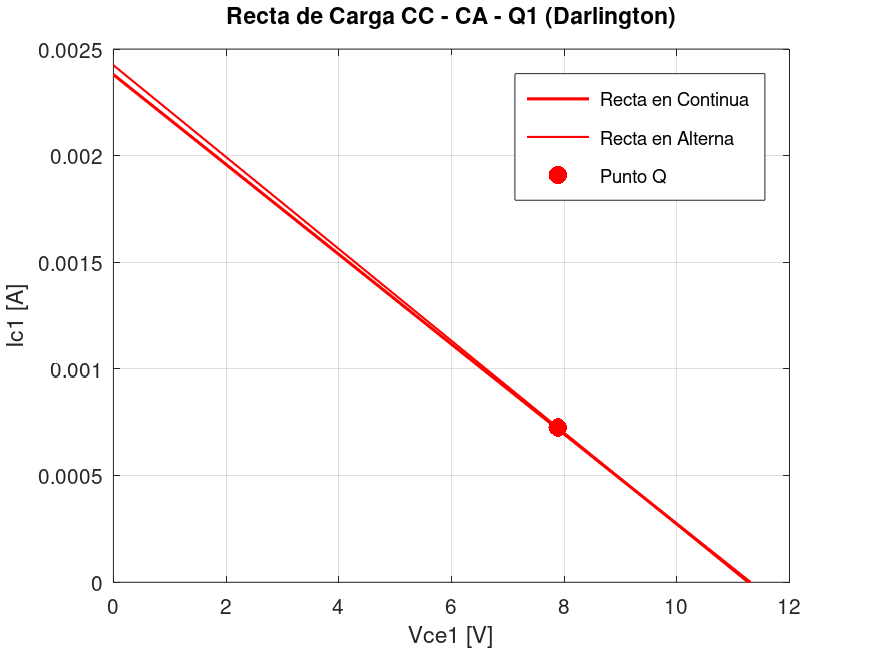
\includegraphics[width=\linewidth]{Imagenes/RectaQ1.png}
    \caption{Rectas de carga de Q1}
    \label{RectaQ1}
  \end{minipage}
  \hfill
  \begin{minipage}{0.48\textwidth}
    \centering
    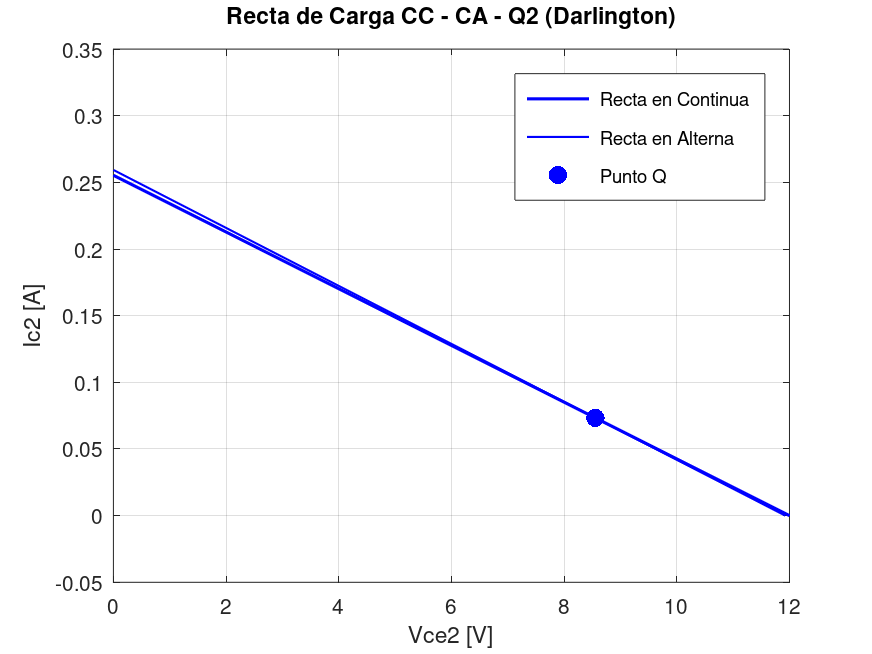
\includegraphics[width=\linewidth]{Imagenes/RectaQ2.png}
    \caption{Rectas de carga de Q2}
    \label{RectaQ2}
  \end{minipage}
\end{figure}

\begin{figure}[H]
  \centering
  \resizebox{250}{!}{
  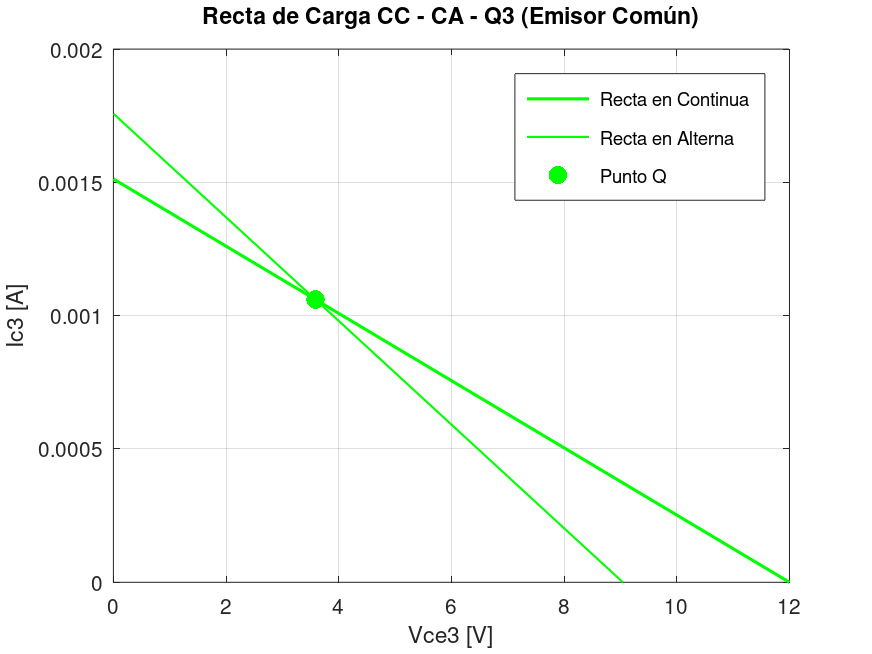
\includegraphics{Imagenes/RectaQ3.png}
  }
  \caption{Rectas de Carga de Q3}
  \label{RectaQ3}
\end{figure}

\begin{figure}[H]
  \centering
  \begin{minipage}{0.48\textwidth}
    \centering
    \resizebox{250}{!}{
      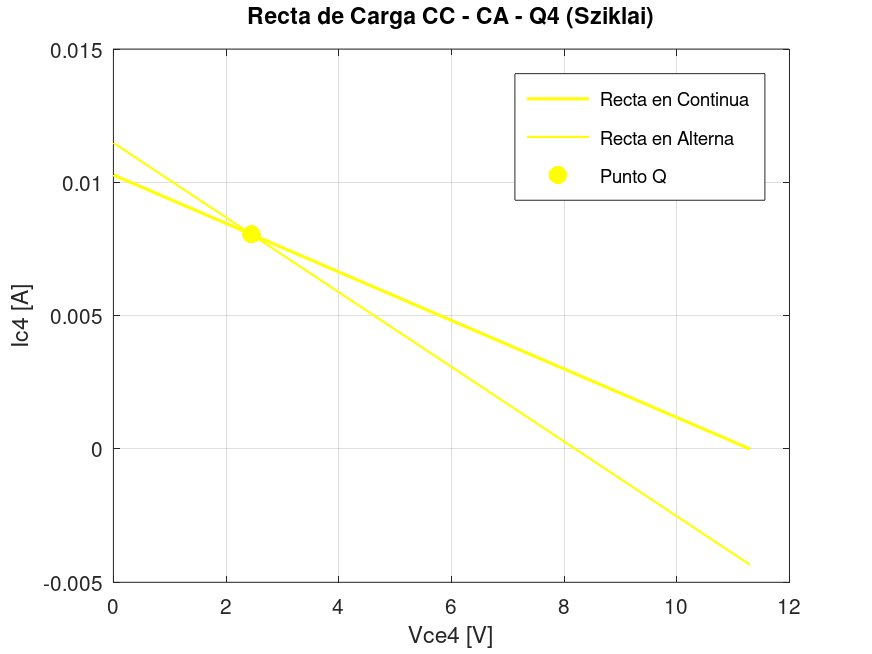
\includegraphics{Imagenes/RectaQ4.png}
    }
    \caption{Rectas de Carga de Q4}
    \label{RectaQ4}
  \end{minipage}
  \hfill
  \begin{minipage}{0.48\textwidth}
    \centering
    \resizebox{250}{!}{
      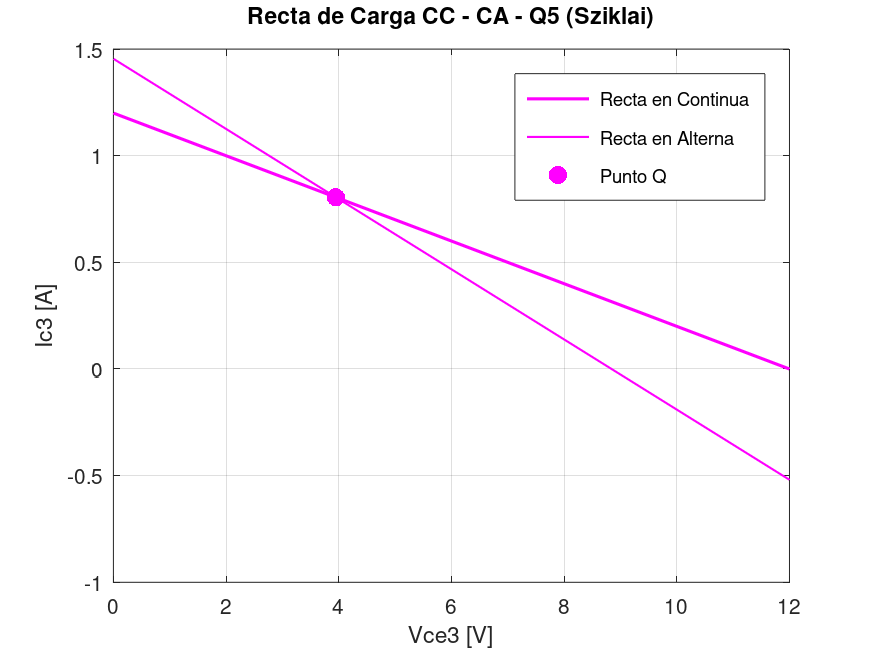
\includegraphics{Imagenes/RectaQ5.png}
    }
    \caption{Rectas de Carga de Q5}
    \label{RectaQ5}
  \end{minipage}
\end{figure}

En estas rectas se puede ver que los componentes calculados con anterioridad dejan a los transistores polarizados en puntos alejados de la seturación ($v_{ce} = 0$) y corte ($v_{ce} = Alimentación$) y, si bien no de manera exacta, cerca de la máxima excursión simétrica. 

Para esto último la que es de mayor interés es la recta del Emisor Común (\cref{RectaQ3}), ya que es esta la etapa amplificadora en el diseño y, como se aprecia en la figura, tiene una gran capacidad de escursión, lo que permite amplificar señales de mayor amplitud.

También es posible ver que, como era previsible, el amplificador Darlington (\cref{RectaQ1} y \cref{RectaQ2}) no tiene variación efectiva en alterna. Esto es porque posee una amplificación unitaria, lo cual no afecta al diseño ya que su porpósito es dar una alta impedancia de entrada al circuito.

Una aclaración importante en este punto es que el amplificador Sziklai por si solo (midiendo su ganancia en el nodo de $R_{ES}$) tiene un valor de ganancia ligeramente menor a uno, sin embargo, tiene una impedancia de salida muy pequeña (en el orden de los $m\Omega$), por lo que se implementó la $R_O$ para aumentar esa impedancia de salida y que alcanze los ocho Ohms. 

Esto tiene el efecto de, al medir la ganancia en el verdadero punto de salida del amplificador (luego de $R_O$), esta se vea dividida aproximadamente por un factor de dos en este caso. Esto porque al circuito se lo está cargando con una impedancia $R_L$ muy similar a esta $R_O$, creando un divisor de tensión con impedancias similares.

Continuando con el análisis del circuito, se resolvió el modelo de pequeña señal simplificado (\cref{fig:AmpTotPS}) para obtener un valor total de ganancia y los modelos de cada etapa (\cref{fig:Dar_PS}, \cref{fig:EMPS} y \cref{fig:SzPS}) para obtener la ganancia teórica de cada una.

EL circuito final del amplificador (\cref{AmpconC}) fue resuelto de manera iterativa para obtener los distintos valores de ganancia en función de la frecuencia, lo que también permite hacer una corroboración del valor teórico obtenido, y los valores de tensión de salida para un conjunto de tensiones de entrada a una dada frecuencia. El gráfico de Bode del amplificador.

\begin{figure}[H]
  \centering
  \resizebox{250}{!}{
    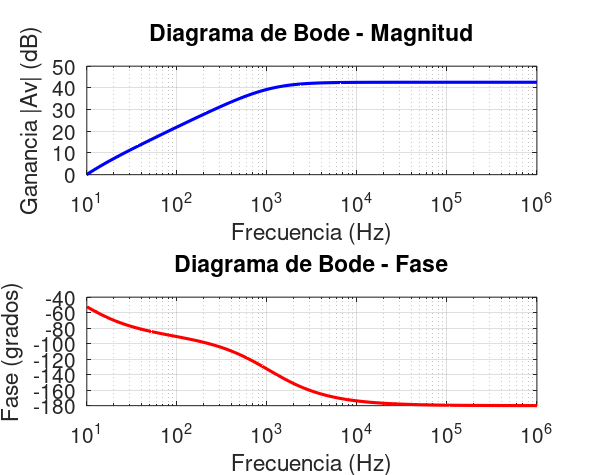
\includegraphics{Imagenes/Bode.png}
  }
  \caption{Magnitud y Fase de la amplificaión teórica}
  \label{Bode}
\end{figure}

Como se puede ver en \cref{Bode}, la canancia toma, en las frecuencias mayores a $2kHz$ que es la zona apropiada de operación del circuito, un valor de ganancia estable de una magnitud suficiente. Además se puede ver el efecto de desfasaje de 180 grados causado por el amplificador Emisor Común. Con estas comprobaciones hechas se pasó a la etapa de simulación para corroborar el funcionamiento adecuado del amplificador.

Si bien hay cálculos que no son apropiados hacer en la etapa de diseño, sino en la de simulación, como los límites de linealidad, ya que se requiere justamente de la simulación de los efectos parásitos de los componentes, si se pueden hacer los cálculos de potencia de los componentes y verificar que aquellos selecionados operen dentro de su zona segura (verificaión de los Absolute Maximum Ratings).

Los resultados de las potencias calculadas, siimulads y medidas se presentarán más adelante, a continuación se presentan los componentes seleccionados, su zona de trabajo en el diseño y sus rangos máximos, obtenidos de las correspondientes hojas de datos.

\begin{table}[H]
  \centering
  \begin{tabular}{|c|c|c|}
    \hline
    Componente & Potencia de Diseño [mW] & Potencia Máxima [mW] \\ \hline
    R_{BD} & 0.051 & 250 \\ \hline
    R_{ED} & 252.7 & 250 \\ \hline
    R_{1E} & 0.799 & 250 \\ \hline
    R_{2E} & 0.141 & 250 \\ \hline
    R_{CE} & 7.497 & 250 \\ \hline
    R_{EE} & 1.350 & 250 \\ \hline
    R_{1S} & 3.132 & 250 \\ \hline
    R_{2S} & 3.698 & 250 \\ \hline
    R_{ES} & 6483  & 10000 \\ \hline
    R_{CB} & 6.354 & 250 \\ \hline
    R_O    & 39.02 & 250 \\ \hline
    R_L    & 41.62 & 250 \\ \hline
    Q1 BC546B & 5.7264 & 500 \\ \hline
    Q2 BD139  & 627.2  & 8000 \\ \hline
    Q3 BC546B & 3.8043 & 500 \\ \hline
    Q4 TIP122 & 19.736 & 2000 \\ \hline
    Q5 TIP127 & 3178.8 & 65000 \\ \hline
  \end{tabular}
\end{table}

En algunos casos, si bien el componente es capaz de soportar la potencia disipada, es necesario colocar un disipador (esto está esecificado también en la hoja de datos de los componentes utilizados).

En particular, si bien Q4 y Q5 pertenecen a la misma familia de transistores y tienen el mismo encapsulado, Q5 requiere de disipador y Q4 no. Esto debido a que, como se ve en la tabla, la potencia de disipasión máxima de Q4 son 2 W, esto es sin disipador. Como Q5 supera ese valor en su potencia de diseño, es necesario utilizar un disipador en este componente.

Ya que esta cota no es sueprada excecivamente, se optó por utilizar el disipador estandar del encapsulado TO220 (el que corresponde a estos transistores).

Para corroborar que los transistores estuvieran siendo utilizados dentro de los rangos establecidos por sus Absolute Maximum Ratings se utilizaron las hojas de datos de estos componentes (\cite{tip122}, \cite{bd139}, \cite{bc546}).

\subsubsection{Diseño de PCB}

  Tomando el diseño visto en \cref{fig:AmpTot}, se utilizó el programa KiCAD para el diseño de la placa montada. Adicionalmente al diseño se le implementaron:
\begin{enumerate}
  \item Jumpers de aislación de etapas
  \item Test Points para la mediciones de  y corriente
  \item 2 headers macho a 90 grados para conectores BNC de entrada y salida
  \item Bornera doble de alimentación
  \item Capacitor de $1000_{\mu \text{F}}$ previo a $R_L$
  \item 2 Headers macho a GND para fichas cocodrilo
\end{enumerate}

Se tuvieron en cuenta las mediciones de la consigna para posicionar los puntos de prueba en el circuito, se optó por omitir aquellos Test Points en lugares donde los componentes de montaje brinden el espacio para su prueba con el fin de obtener un diseño más compacto y de menor costo.

\vspace{0.5em}
{\small\textbf{Diseño de Esquemático}}

Una vez constituido el esquemático (\cref{Esquematico}) a utilizar se le asignaron las huellas de los componentes, estas fueron designadas según la disipación de potencia estimada.

\begin{figure}[H]
  \centering
  \resizebox{\textwidth}{!}{
    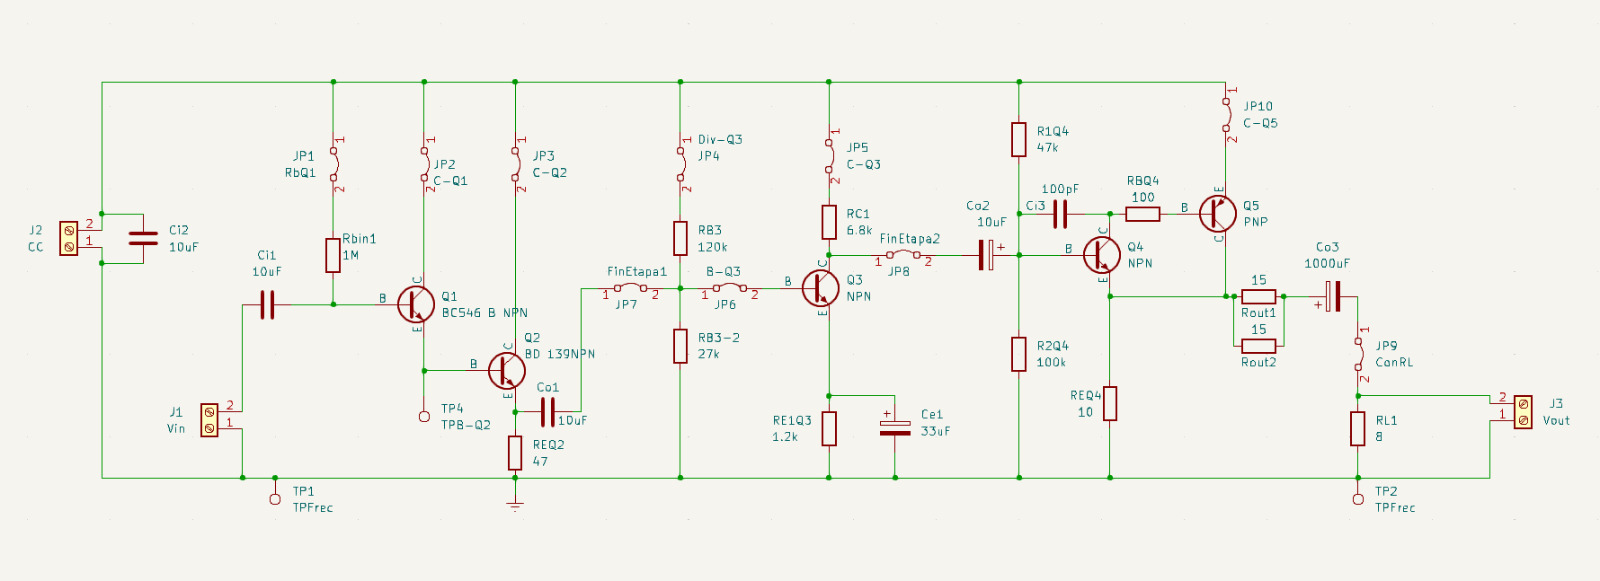
\includegraphics{Imagenes/Esquemático.jpeg}
  }
  \caption{Esquemático del diseño final}
  \label{Esquematico}
\end{figure}

\vspace{0.5em}
{\small\textbf{Diseño de PCB }}

Para el enrutamiento (\cref{Trazas}) de los componentes y su disposición se tuvieron en cuenta diversos factores:

\begin{enumerate}
  \item El ancho de vía de potencia: $1.5_{mm}$
  \item Ancho de vía general: $1_{mm}$
  \item Espaciado de los alrededores de Q2 y Q5 para disipador
  \item Separación entre la $R_{ES}$ y los transistores 
  \item Jumpers de fin de etapa en posición horizontal
  \item Polaridad de los header a 90 grados según la bornera BN
  \item Jumpers ubicados en el exterior de la placa
  \item Plano de GND rodeando el circuito
  \item Conexión de componentes mediante la capa B.Cu (Bottom Copper) 
  \item Zonas de relleno con conexión a tierra, alivios térmicos y separación de contornos de $0.3_{mm}$
  \item Dimensiones de placa $46.5_{cm^2}$
  \item Puntos de medición de tensión en simetría
  \item Uso de ángulos a 45 grados para evitar la discontinuidad en la impedancia característica de la pista, estrés y el efecto de “Trampa de ácido” por tensión superficial
\end{enumerate}

\begin{figure}[H]
  \centering
  \resizebox{350}{!}{
      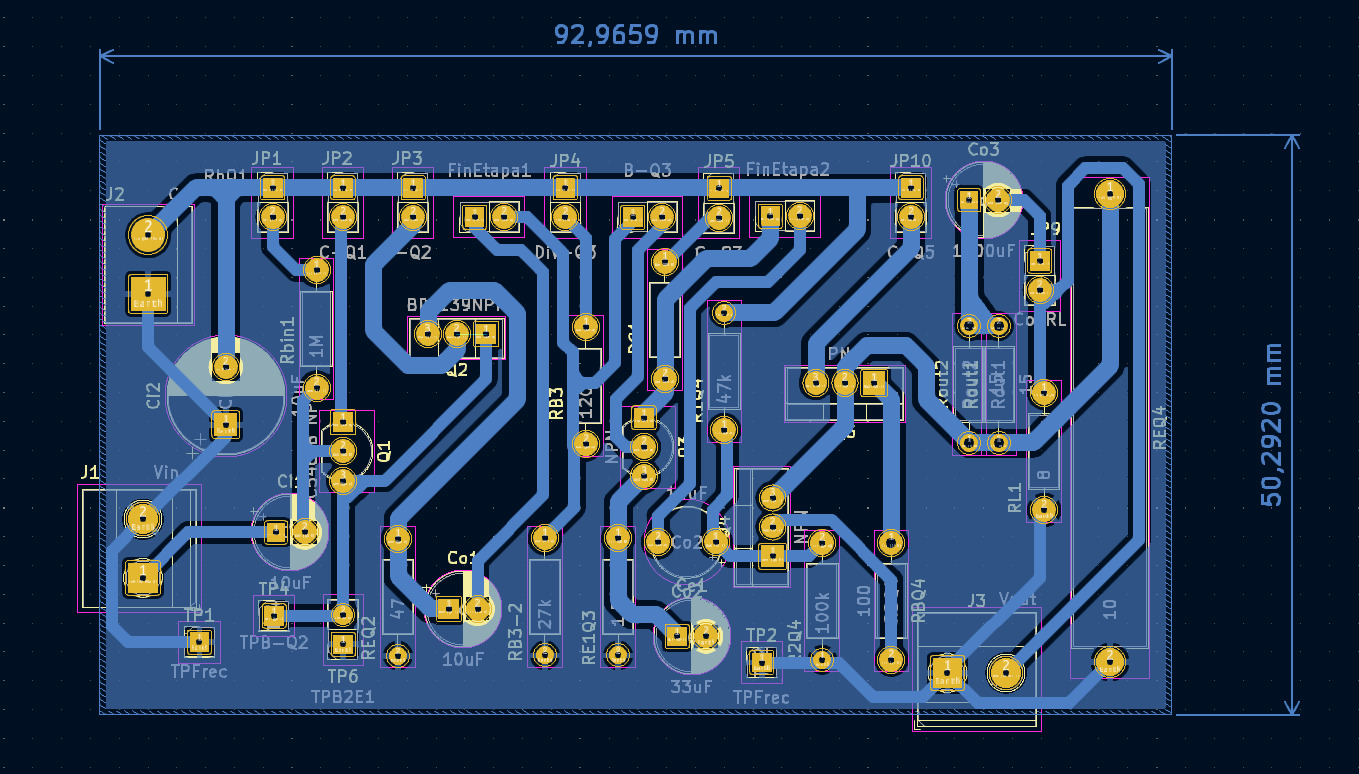
\includegraphics{Imagenes/Trazas.jpeg}
  }
  \caption{Vista del Bottom Copper del diseño}
  \label{Trazas}
\end{figure}

Problemáticas presentes:
\begin{enumerate}
  \item Todas las huellas de los transistores, sin importar el encapsulado, mantienen la misma distribución de pines (Base=2, Colector=1 y Emisor=3), hecho que en la realidad difiere en los encapsulados TO-126 y TO-220, esto puede presentar problemas en el momento de su enrutamiento y funcionamiento en placa montada.
  \item Las huellas de los capacitores tienen una orientación de polarización indistinta, lo que presenta problemas en su comportamiento esperado.
  \item Las huellas de las entradas BNC tienen una orientación dada.
\end{enumerate}

\vspace{0.5em}
{\small\textbf{Diseño de Impresión }}

A continuación se presenta el diseño (\cref{Impreso}) utilizado para transferir las pistas a la placa de cobre

\begin{figure}[H]
  \centering
  \resizebox{350}{!}{
    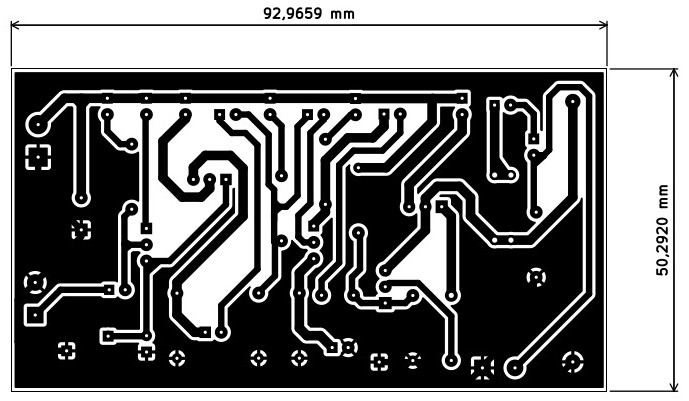
\includegraphics{Imagenes/Impreso.jpeg}
  }
  \caption{Diseño de Impresión final}
  \label{Impreso}
\end{figure}

\subsection{Simulación}

%\section{SECCIÓN: SIMULACIÓN EN LTSPICE}

\subsubsection{Fundamentación de Directivas SPICE Empleadas}
Para la caracterización del amplificador multietapa se empleó el entorno de simulación \textbf{LTspice®}. Con el objetivo de automatizar y estandarizar la obtención de parámetros eléctricos, se utilizaron las siguientes directivas fundamentales de forma genérica:

\begin{itemize}
    \item \texttt{.op} \textbf{(Punto de Operación DC):} Evalúa las tensiones continuas de nodo y corrientes de rama sin señal aplicada, permitiendo verificar la zona de trabajo activa de los semiconductores y su disipación de potencia estática.
    \item \texttt{.ac <type> <n> <fstart> <fstop>} \textbf{(Análisis de Pequeña Señal AC):} Realiza un barrido frecuencial de pequeña señal para obtener la respuesta en frecuencia (Diagrama de Bode), ganancias de tensión e impedancias complejas de entrada y salida ($Z_{in}$, $Z_{out}$).
    \item \texttt{.tran <tstep> <tstop>} \textbf{(Análisis Temporal de Transitorios):} Simula la respuesta temporal dinámica del circuito en el dominio del tiempo frente a señales senoidales para evaluar la forma de onda, excursiones pico a pico y simetría de salida.
    \item \texttt{.noise V(node) <src> <type> <n> <fstart> <fstop>} \textbf{(Análisis de Ruido):} Calcula la Densidad Espectral de Potencia (PSD) de ruido térmico y de disparo referida a la salida o entrada del circuito.
    \item \texttt{.four <freq> V(out)} \textbf{(Análisis de Fourier):} Procesa la señal temporal del análisis \texttt{.tran} aplicando la Transformada Rápida de Fourier (FFT) para calcular la Distorsión Armónica Total (THD) evaluando hasta el 9no armónico respecto a la componente fundamental.
    \item \texttt{.step param <var> list <val1> <val2>...} \textbf{(Análisis Paramétrico):} Ejecuta simulaciones iterativas variando parámetros como la amplitud de entrada ($A_{in}$), la impedancia de carga ($R_L$) o las tensiones de alimentación ($V_{CC}$) para determinar analíticamente los límites de operabilidad y estabilidad lineal observando la deformación o recorte de la señal en la salida.
    \item \texttt{.meas <type> <name>  FIND <expr> AT/WHEN <cond>} \textbf{(Mediciones Condicionales con FIND):} Permite extraer valores exactos de magnitudes eléctricas (tensiones, corrientes, impedancias o desfases) evaluados en puntos o frecuencias específicas (por ejemplo, evaluar la ganancia o impedancia exactamente a $1\,\text{kHz}$ mediante \texttt{.meas AC Zin FIND Mag(V(in)/I(Vin)) AT=1k}).
\end{itemize}
\subsubsection{Modelos SPICE de Transistores Empleados}
Para garantizar una simulación acorde a los transistores reales utilizados, se incorporaron al esquema las siguientes directivas de modelo de parámetros SPICE para los semiconductores NPN y PNP:

\begin{lstlisting}
* Modelo TIP122 
.model Q5 PNP (IS=1e-11 BF=1000 VAF=100 IKF=3 ISE=1e-10 NE=2 BR=4 VAR=20 RB=10 RC=0.1 CJE=1.2e-9 CJC=2.5e-10 VCEO=100 ICN=5)

* Modelo BD139
.model Q2 NPN (IS=2.39e-13 BF=200 VAF=100 IKF=0.8 ISE=1e-14 NE=1.5 BR=3 VAR=20 RB=1.5 RC=0.15 CJE=2e-10 CJC=8e-11 VCEO=80 ICN=1.5)

* Modelo BC546
.model Q1 NPN (IS=1.8e-14 BF=400 VAF=100 IKF=0.15 ISE=5e-15 NE=1.25 BR=5 VAR=20 RB=20 RC=0.6 CJE=1.3e-11 CJC=4.5e-12 VCEO=65 ICN=0.1)

* Modelo BC546
.model Q3 NPN (IS=1.8e-14 BF=400 VAF=100 IKF=0.15 ISE=5e-15 NE=1.25 BR=5 VAR=20 RB=20 RC=0.6 CJE=1.3e-11 CJC=4.5e-12 VCEO=65 ICN=0.1)
\end{lstlisting}
% =========================================================================
% APARTADO 1: GLOBAL
% =========================================================================
\subsubsection{Análisis Global del Amplificador (Simulación Integral)}

%\subsection*{Prueba y Caracterización General del Sistema Completo}
En esta sección se consolida la evaluación del amplificador de 3 etapas interconectado en cascada cargado nominalmente con $R_L = 8\,\Omega$ (\cref{fig:circuito_global}).

\begin{figure}[H]
    \centering
    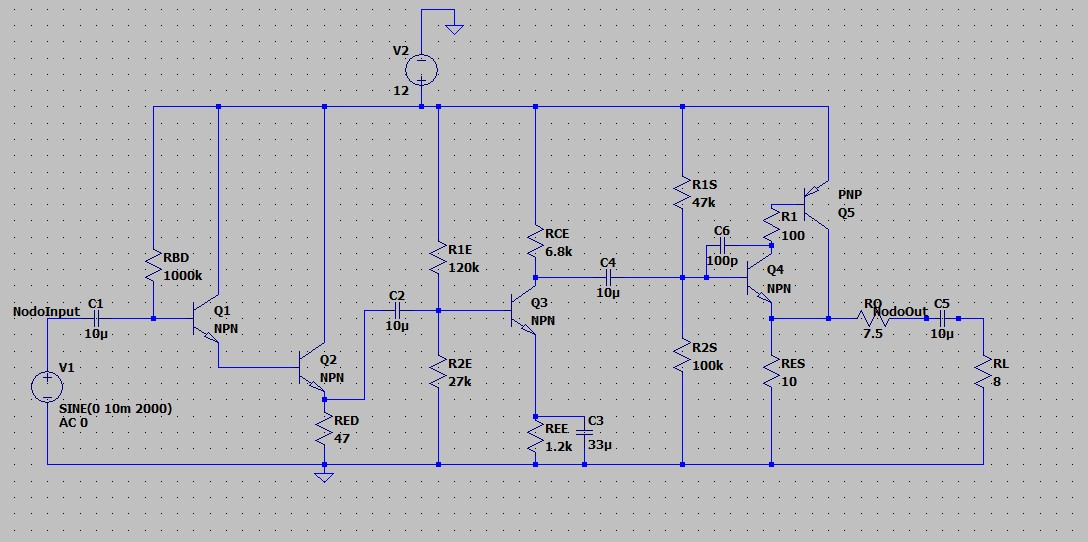
\includegraphics[width=0.85\linewidth]{Simu/Modelo_spice.jpg}
    \caption{Esquemático completo del amplificador en LTspice.}
    \label{fig:circuito_global}
\end{figure}

\vspace{0.5em}
{\small\textbf{Polarización y Disipación de Potencia Global (.op)}}

%\subsubsection{1.1. Polarización y Disipación de Potencia Global (.op)}
Se ejecuta la simulación \texttt{.op} para registrar los niveles de tensión en todos los nodos de la red y la corriente consumida desde la fuente principal $V_2 = 12\,\text{V}$ (\cref{PuntoOP}).
\begin{figure}[H]
    \centering
    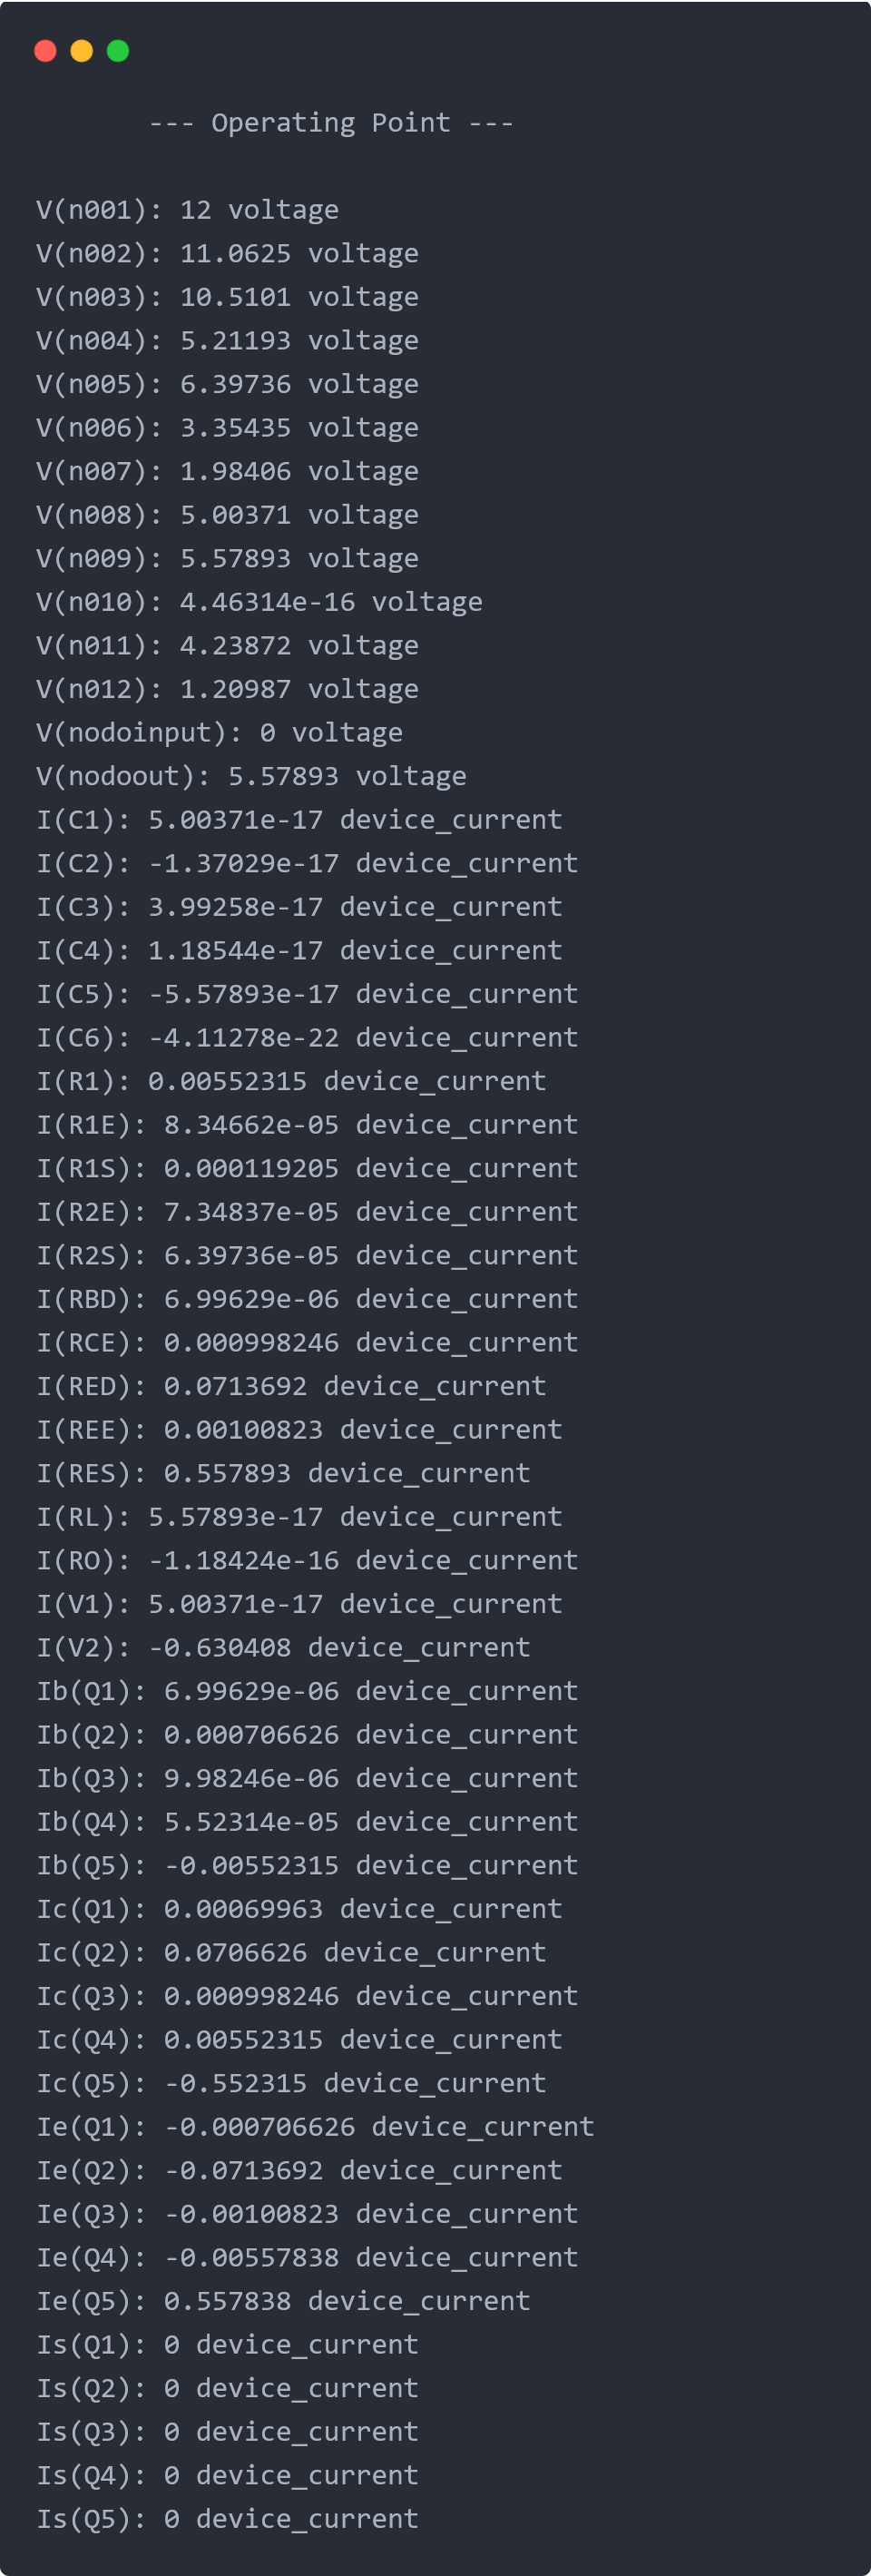
\includegraphics[width=0.5\linewidth]{Simu/OpTotal.png}
    \caption{Punto de operación.}
  \label{PuntoOP}
\end{figure}

\vspace{0.5em}
{\small\textbf{Impedancia de Entrada Total ($Z_{in}$)}}

%\subsubsection{1.2. Impedancia de Entrada Total ($Z_{in}$)}
Se mide aplicando un análisis \texttt{.ac} y calculando la relación entre la tensión en el nodo de entrada y la corriente entregada por la fuente $V_1$: $Z_{in} = \frac{V(\text{NodoInput})}{I(V1)}$ (\cref{SimuZin}).
\begin{figure}[H]
    \centering
    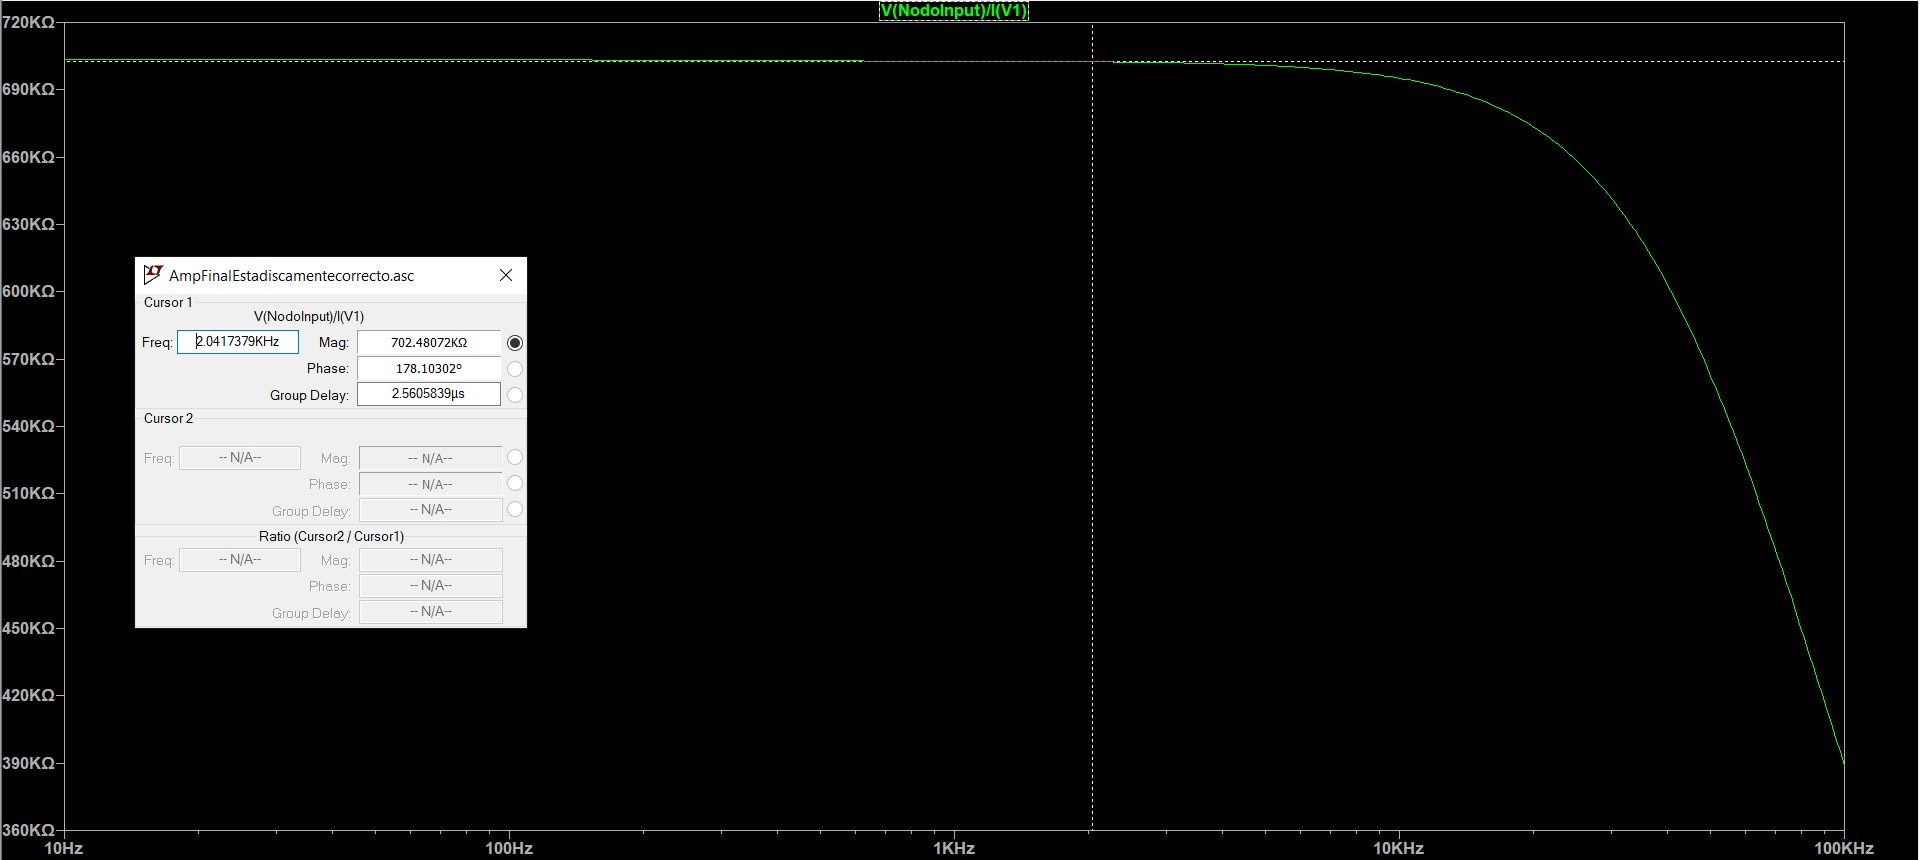
\includegraphics[width=0.75\linewidth]{Simu/Impedancia_Entrada_Total.jpg}
    \caption{Curva de la impedancia de entrada total del amplificador respecto a la frecuencia.}
  \label{SimuZin}
\end{figure}

\vspace{0.5em}
{\small\textbf{Impedancia de Salida Total ($Z_{out}$)}}

%\subsubsection{1.3. Impedancia de Salida Total ($Z_{out}$)}
Para medir la impedancia de salida global, se pasiva la fuente de entrada $V_1$ ($0\,\text{V}$ AC) y se aplica una fuente de corriente AC de prueba $I_{out} = 1\,\text{A}$ en el nodo de salida $\text{NodoOut}$, evaluando $Z_{out} = V(\text{NodoOut})$ (\cref{SimuZo}, \cref{SimuZoT}).
\begin{figure}[H]
    \centering
    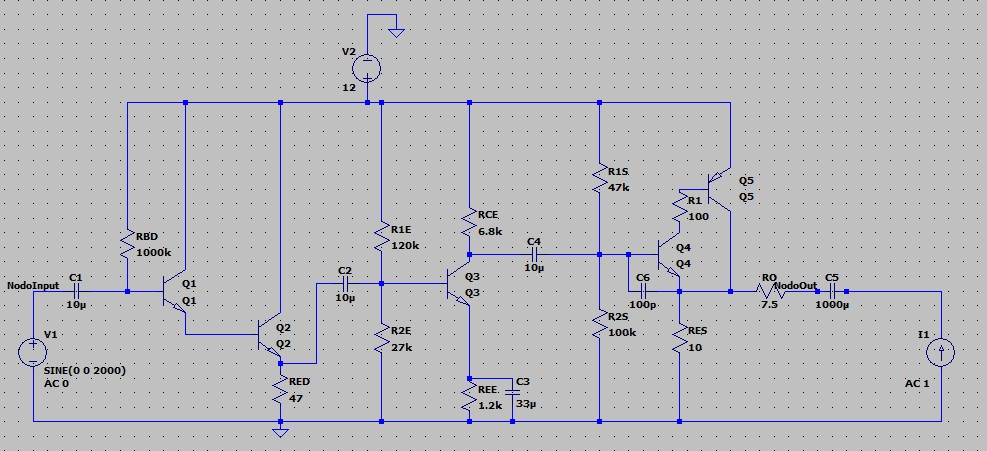
\includegraphics[width=0.75\linewidth]{Simu/Impedancia_Salida_Ciurcuito.jpg}
    \caption{Circuito de como fue medida la impedancia de salida.}
    \label{SimuZo}
\end{figure}
\begin{figure}[H]
    \centering
    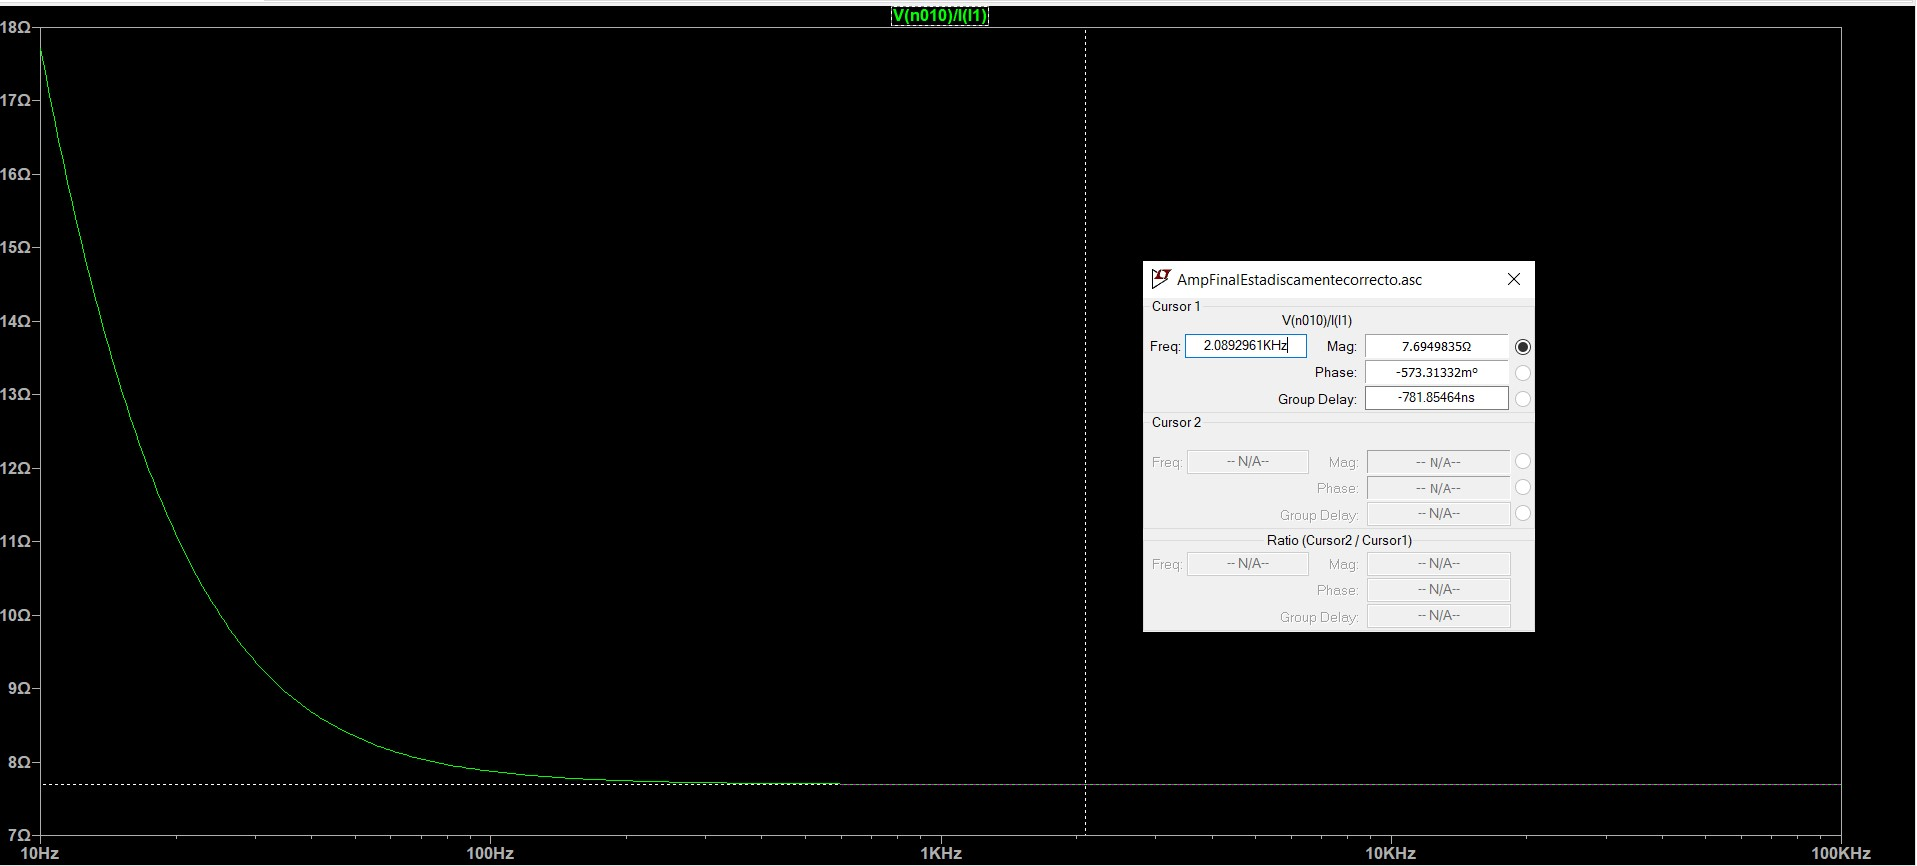
\includegraphics[width=0.75\linewidth]{Simu/Impedancia_Salida_tetal.jpg}
    \caption{Montaje y simulación de la impedancia de salida global $Z_{out}$ del circuito.}
  \label{SimuZoT}
\end{figure}

\vspace{0.5em}
{\small\textbf{Respuesta en Frecuencia AC ($A_v$)}}

%\subsubsection{1.4. Respuesta en Frecuencia AC ($A_v$)}
Análisis del ancho de banda y ganancia total de tensión midiendo $A_v = \frac{V(\text{NodoOut})}{V(\text{NodoInput})}$ (\cref{LimDer}, \cref{LimIz}).
\begin{figure}[H]
    \centering
    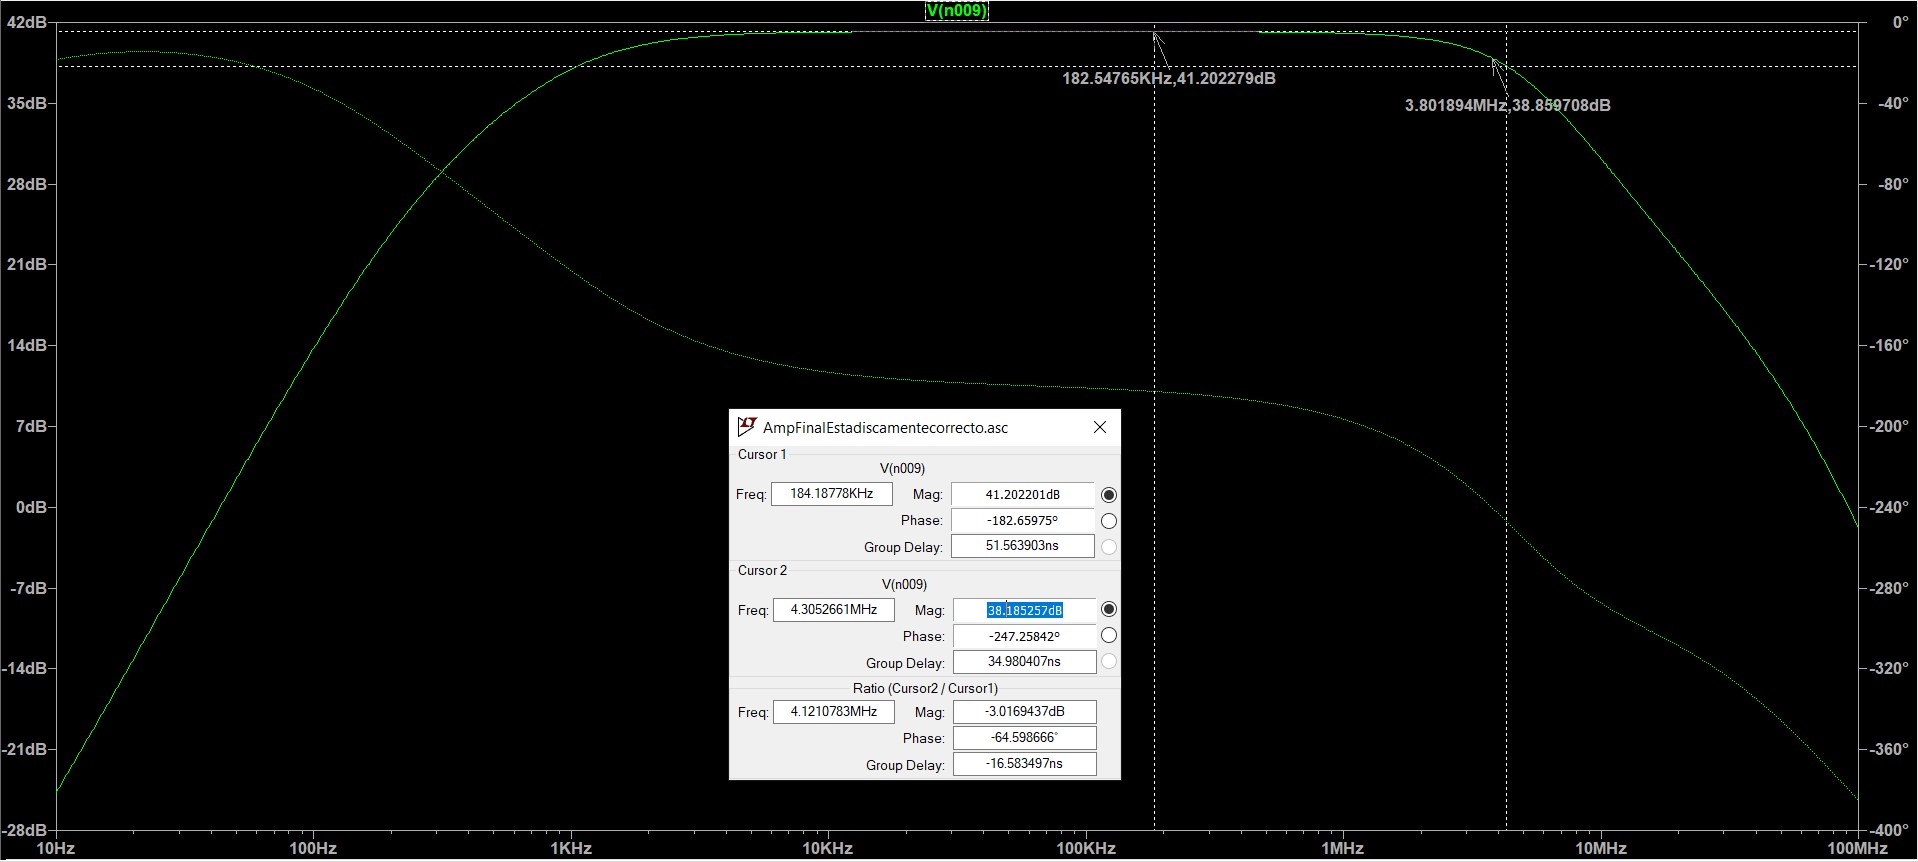
\includegraphics[width=0.75\linewidth]{Simu/BW-LimiteDerecho.jpg}
    \caption{Respuesta en frecuencia con cursor en limite derecho.}
    \label{LimDer}
\end{figure}
\begin{figure}[H]
    \centering
    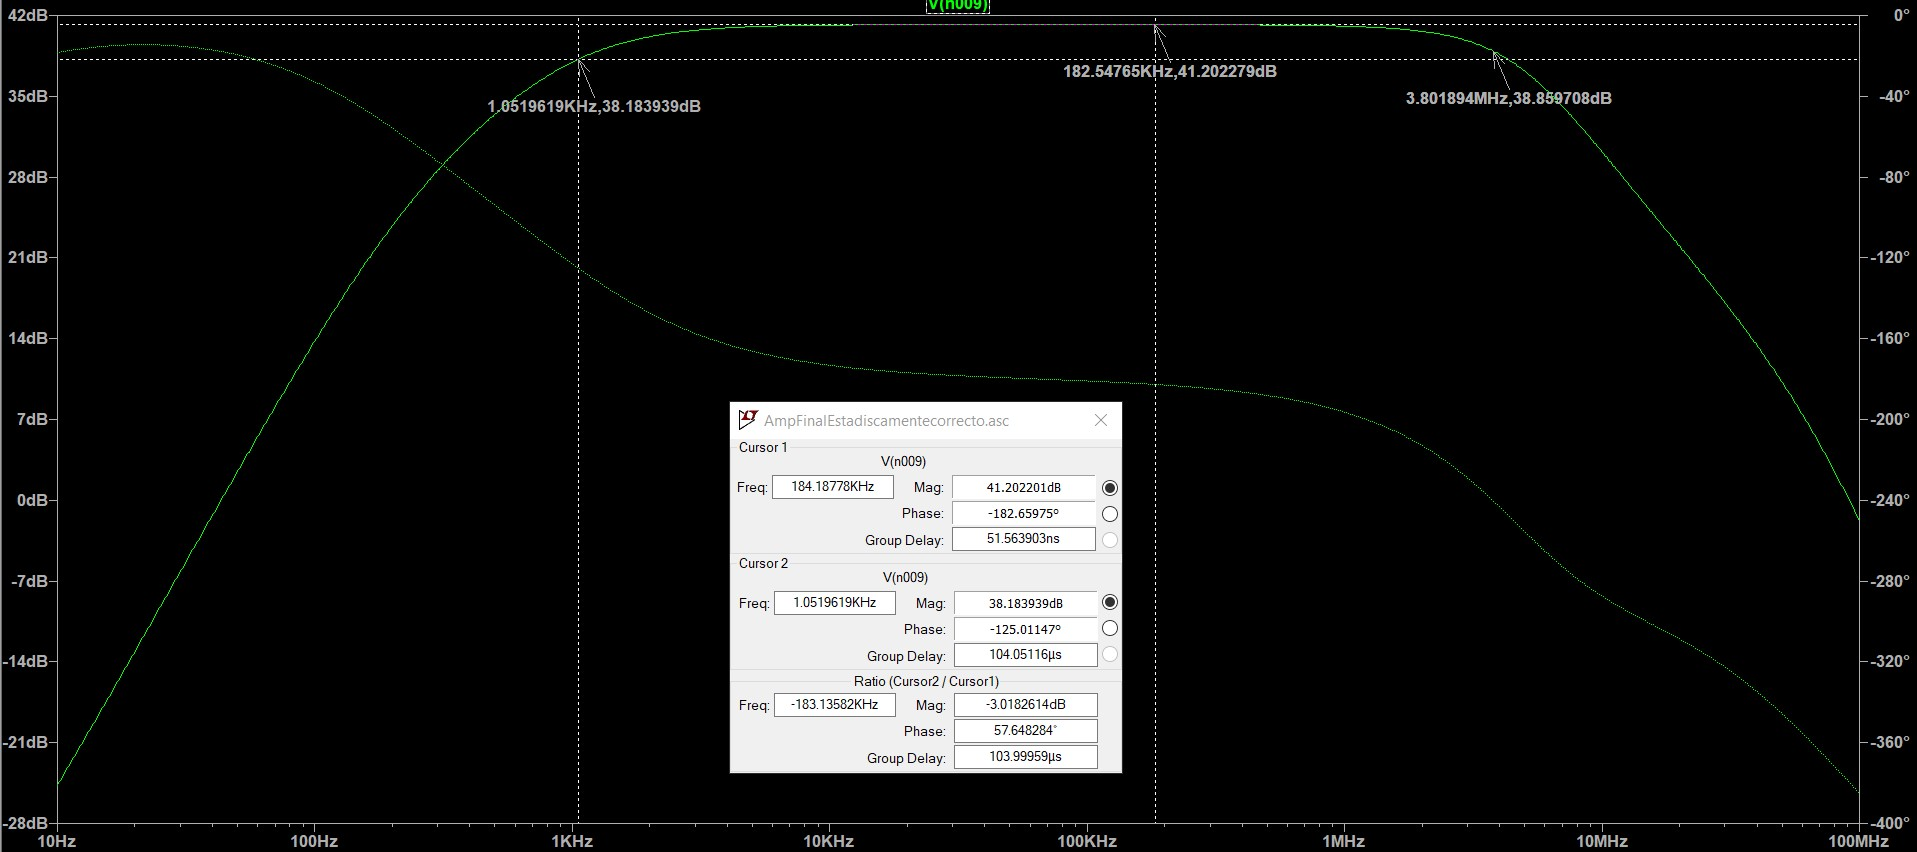
\includegraphics[width=0.75\linewidth]{Simu/BW-LimiteIzquierdo.jpg}
    \caption{Respuesta en frecuencia con cursor en limite izquierdo.}
  \label{LimIz}
\end{figure}

\vspace{0.5em}
{\small\textbf{Respuesta Temporal (.tran)}}

%\subsubsection{1.5. Respuesta Temporal (.tran)}
Respuesta en el dominio del tiempo frente a una entrada senoidal de $5\,\text{kHz}$ e intensidad $10\,\text{mV}_{\text{pico}}$. Se evalúa la excursión de tensión y la simetría de la onda sobre el nodo de salida (\cref{SimuVo}).
\begin{figure}[H]
    \centering
    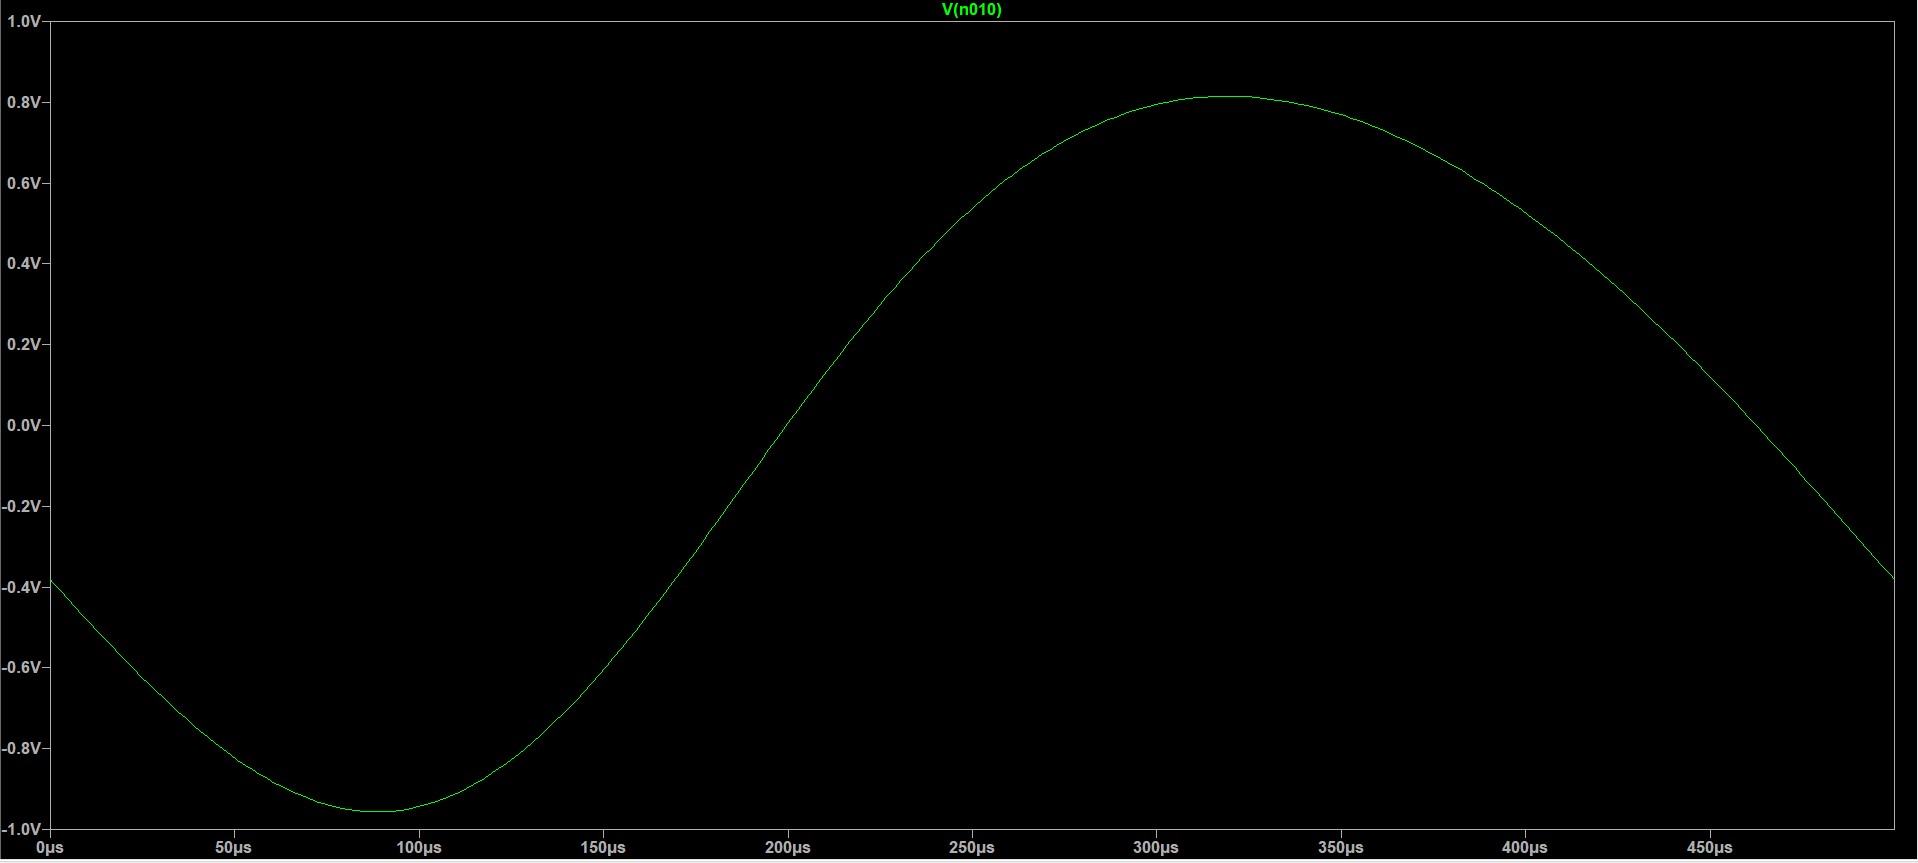
\includegraphics[width=0.75\linewidth]{Simu/Voltaje_salida_10m.jpg}
    \caption{Medición de la respuesta temporal (.tran) de la tensión de salida sobre la carga de $8\,\Omega$.}
  \label{SimuVo}
\end{figure}

\vspace{0.5em}
{\small\textbf{Densidad Espectral de Potencia del Ruido (PSD .noise)}}

%\subsubsection{1.6. Densidad Espectral de Potencia del Ruido (PSD .noise)}
Medición de la PSD de ruido referida a la salida del sistema completo mediante \texttt{.noise V(NodoOut) V1 dec 100 10 100k} (\cref{SimuPSD}, \cref{SimuPSDT}).
\begin{figure}[H]
    \centering
    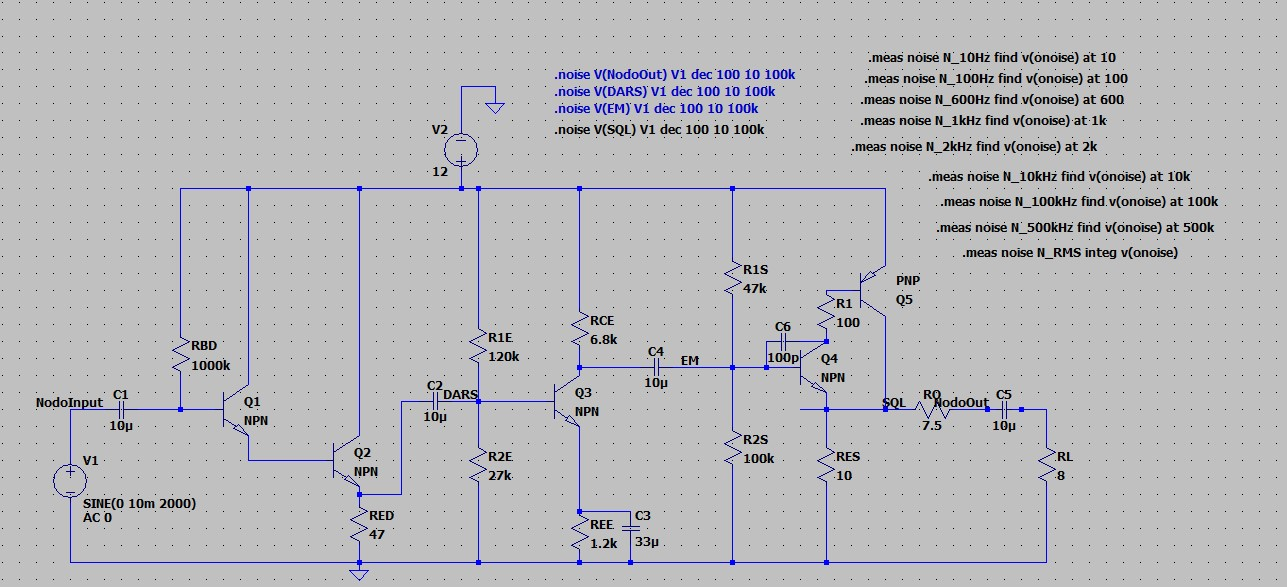
\includegraphics[width=0.75\linewidth]{Simu/Noise-totalcondirct.jpg}
    \caption{Circuito representativo de como se midió el PSD.}
  \label{SimuPSD}
\end{figure}\begin{figure}[H]
    \centering
    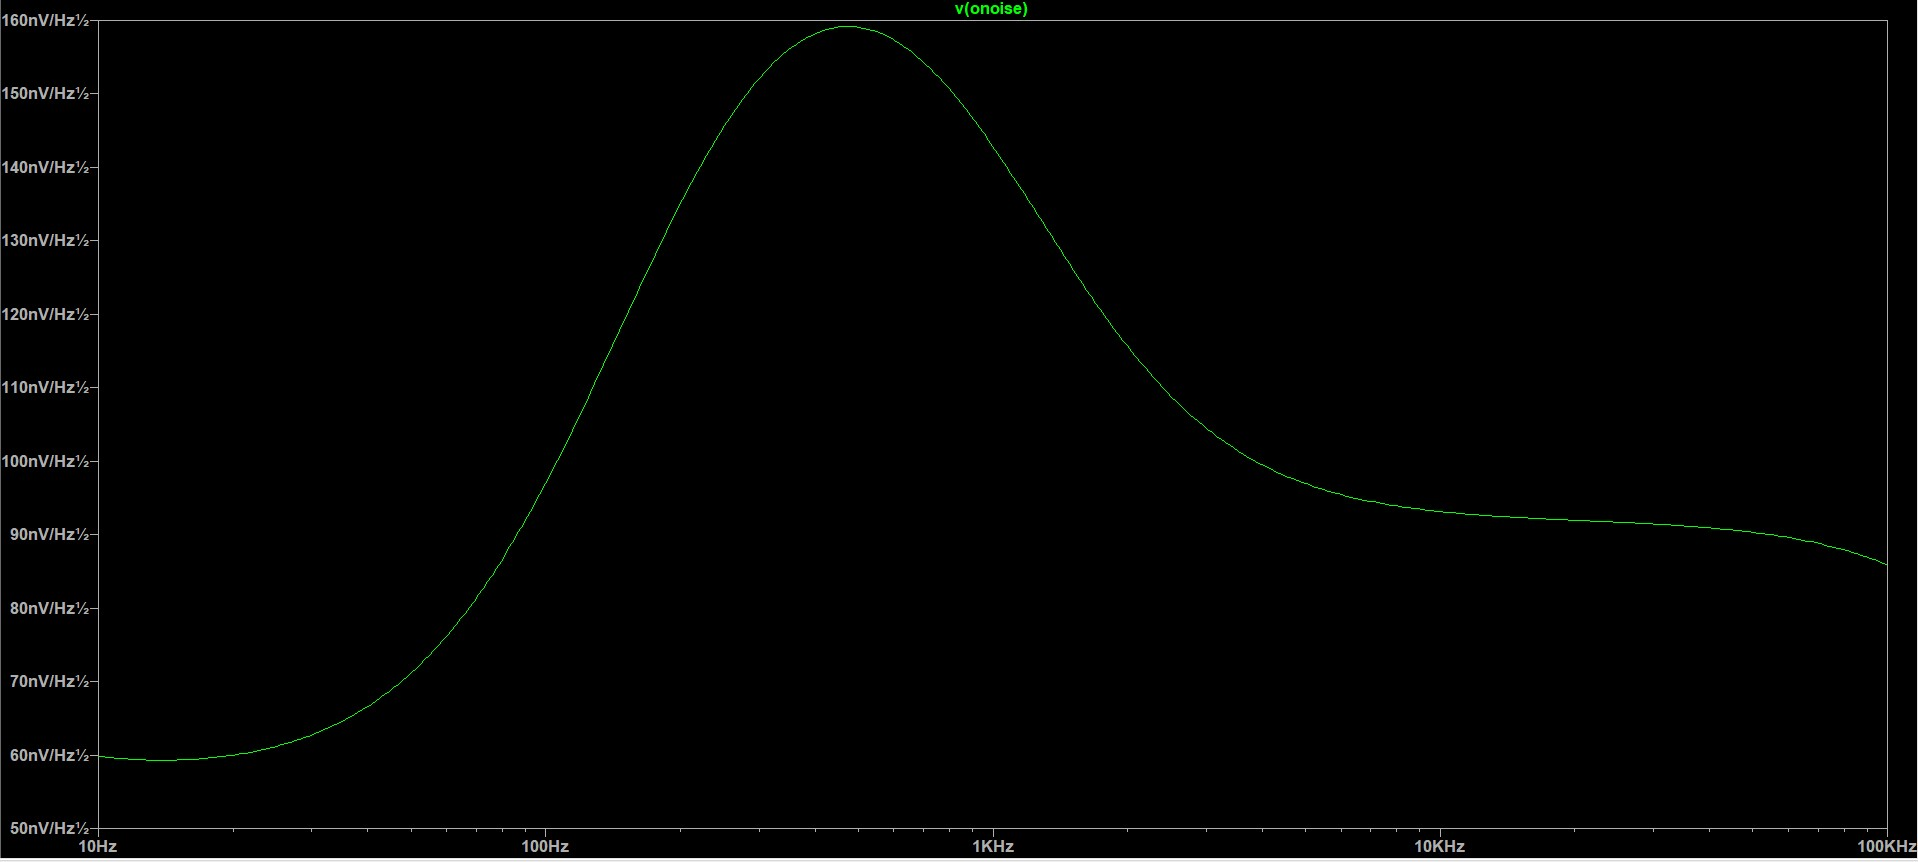
\includegraphics[width=0.75\linewidth]{Simu/Noise-out.jpg}
    \caption{Densidad espectral de potencia del ruido (PSD) total a la salida.}
  \label{SimuPSDT}
\end{figure}

\vspace{0.5em}
{\small\textbf{Distorsión Armónica Total (THD via FFT / .four)}}

%\subsubsection{1.7. Distorsión Armónica Total (THD via FFT / .four)}
Se aplica el análisis de Fourier mediante la directiva \texttt{.four 2000 V(NodoOut)} sobre la señal en la carga $R_L$ a $2\,\text{kHz}$. Los resultados numéricos de distorsión armónica total y la amplitud de las componentes armónicas individuales se inspeccionaron directamente en el registro de salida de LTspice (\textit{Spice Error Log}), al cual se accede mediante la combinación de teclas \textbf{\texttt{Ctrl + L}} tras completar la simulación de transitorios (\cref{THD}).

\begin{figure}[H]
    \centering
    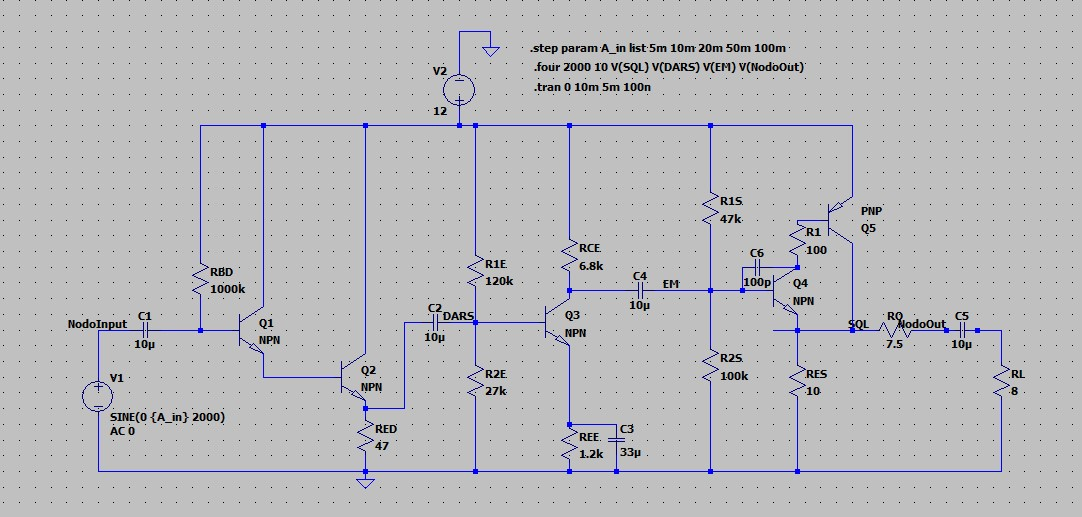
\includegraphics[width=0.75\linewidth]{Simu/Med-THD.jpg}
    \caption{Esquemático y configuración del análisis de Fourier (.four) en LTspice para la inspección de resultados de THD vía Error Log}
  \label{THD}
\end{figure}

\vspace{0.5em}
{\small\textbf{Evaluación de Límites de Operación y Pérdida de Linealidad}}

%\subsubsection{1.8. Evaluación de Límites de Operación y Pérdida de Linealidad}
Para caracterizar con precisión los márgenes dinámicos del amplificador completo y determinar el punto exacto donde se pierde la linealidad (recorte por saturación o corte), se implementaron barridos paramétricos utilizando la directiva \texttt{.step}. Los resultados se estructuran en los siguientes tres análisis:

{\small\textbf{1- Pérdida de Linealidad por Variación de Amplitud de Entrada ($V_{in}$)}}

Mediante el comando \texttt{.step param A\_in list 5m 10m 15m 17m 20m}, se incrementó progresivamente la amplitud de la señal de entrada, observando en la señal de salida el instante exacto en que la forma de onda deja de ser puramente senoidal y comienza el recorte (\cref{PerLinME}. \cref{TransfDin}).

\begin{figure}[H]
    \centering
    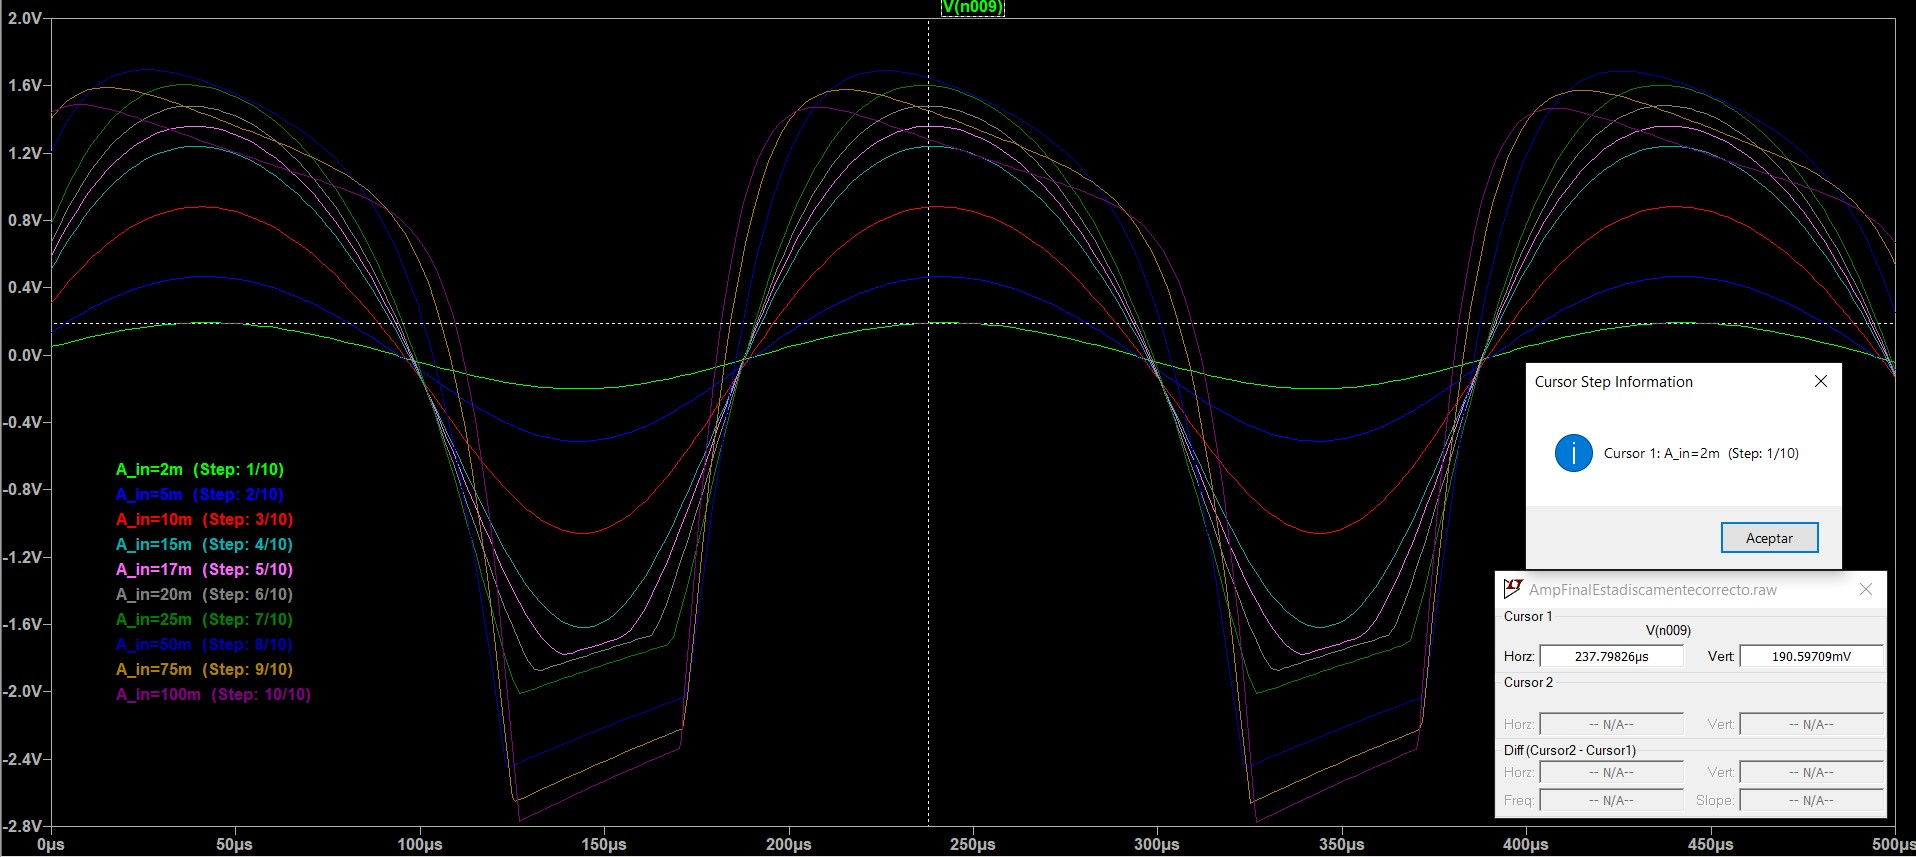
\includegraphics[width=0.75\linewidth]{Simu/Voltaje_salida_5k.jpg}
    \caption{Evaluación de la pérdida de linealidad por excursión máxima de la señal de entrada $V_{in}$.}
  \label{PerLinME}
\end{figure}
\begin{figure}[H]
    \centering
    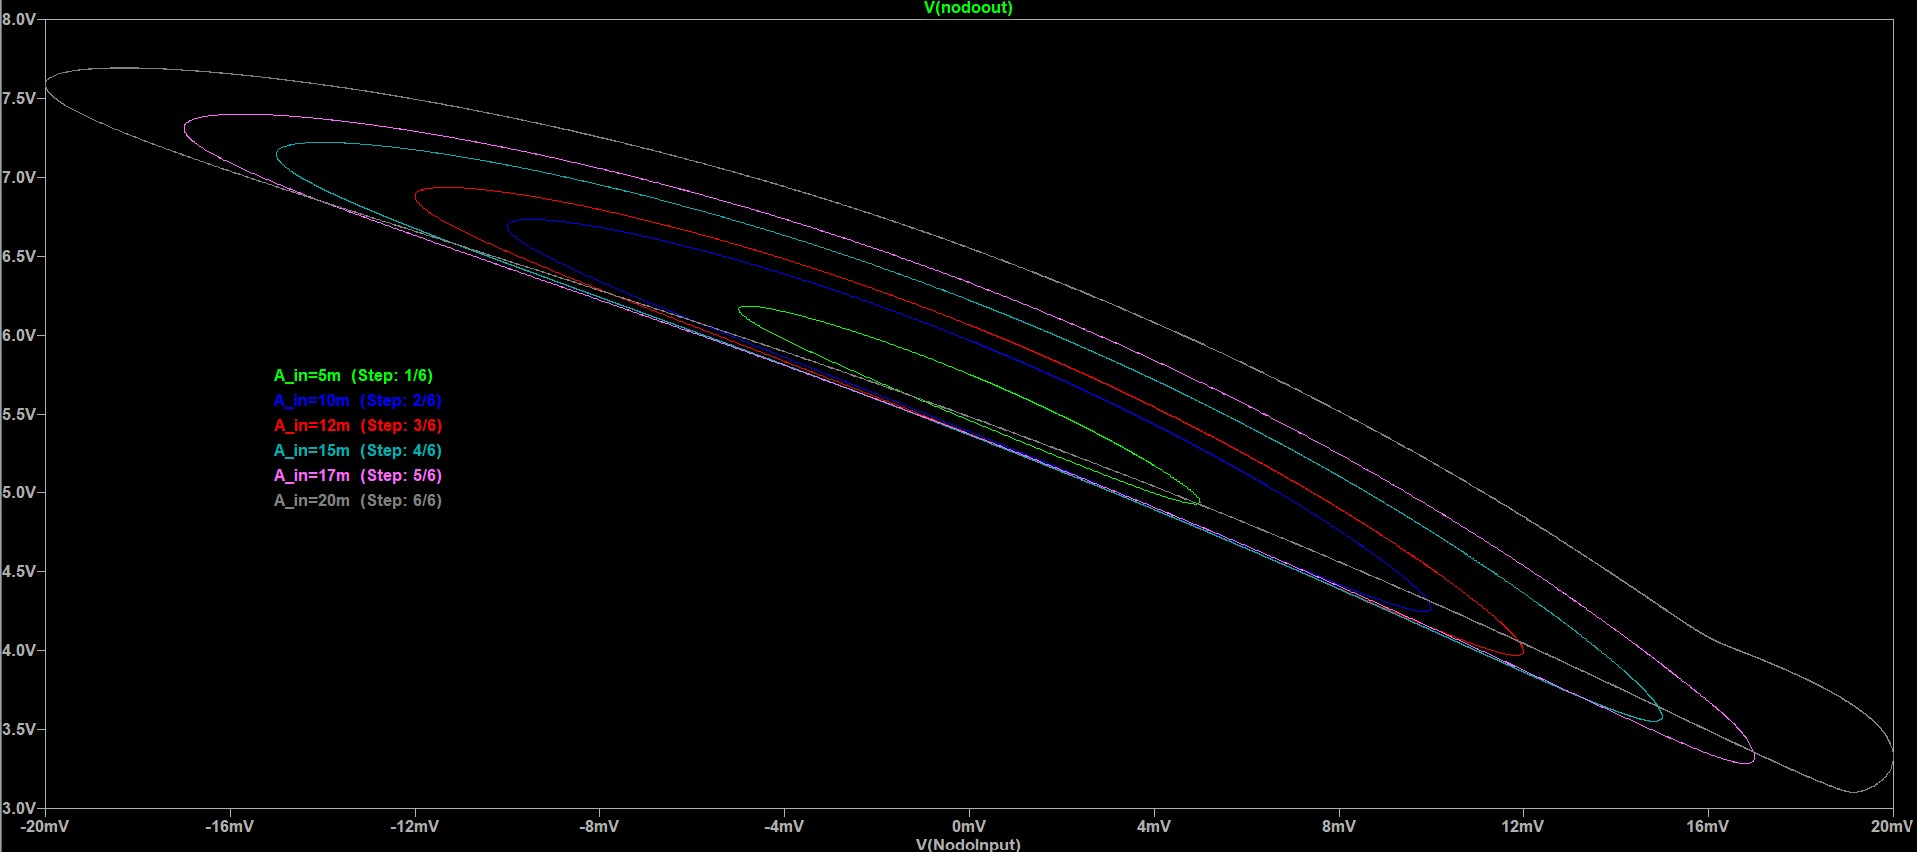
\includegraphics[width=0.75\linewidth]{Simu/Linealidad.jpg}
    \caption{Curva de transferencia dinámica $V(\text{NodoOut})$ vs. $V(\text{NodoInput})$ para diferentes amplitudes de entrada ($A_{in}$ de $5\,\text{mV}$ a $20\,\text{mV}$). La pendiente e inclinación representan la ganancia invertida del sistema, mientras que la deformación progresiva en los bordes para $A_{in} \ge 17\,\text{mV}$ evidencia la pérdida de linealidad y la presencia de distorsión armónica.}
    \label{TransfDin}
\end{figure}

{\small\textbf{2- Límites de Operación por Variación de Alimentación ($V_{CC}$ hacia arriba y hacia abajo)}}

%\paragraph{1.8.2. Límites de Operación por Variación de Alimentación ($V_{CC}$ hacia arriba y hacia abajo)}
Se analizó la tolerancia del amplificador variando la fuente de alimentación $V_2$ ($V_{CC}$) mediante \texttt{.step param VCC 6 18 1}. Esto permitió determinar la tensión mínima de alimentación ($V_{CC,min}$) necesaria para mantener los transistores en región activa y la tensión máxima ($V_{CC,max}$) antes de superar los límites de disipación o distorsión (\cref{BarridoAbajo}, \cref{BarridoArriba}).

\begin{figure}[H]
    \centering
    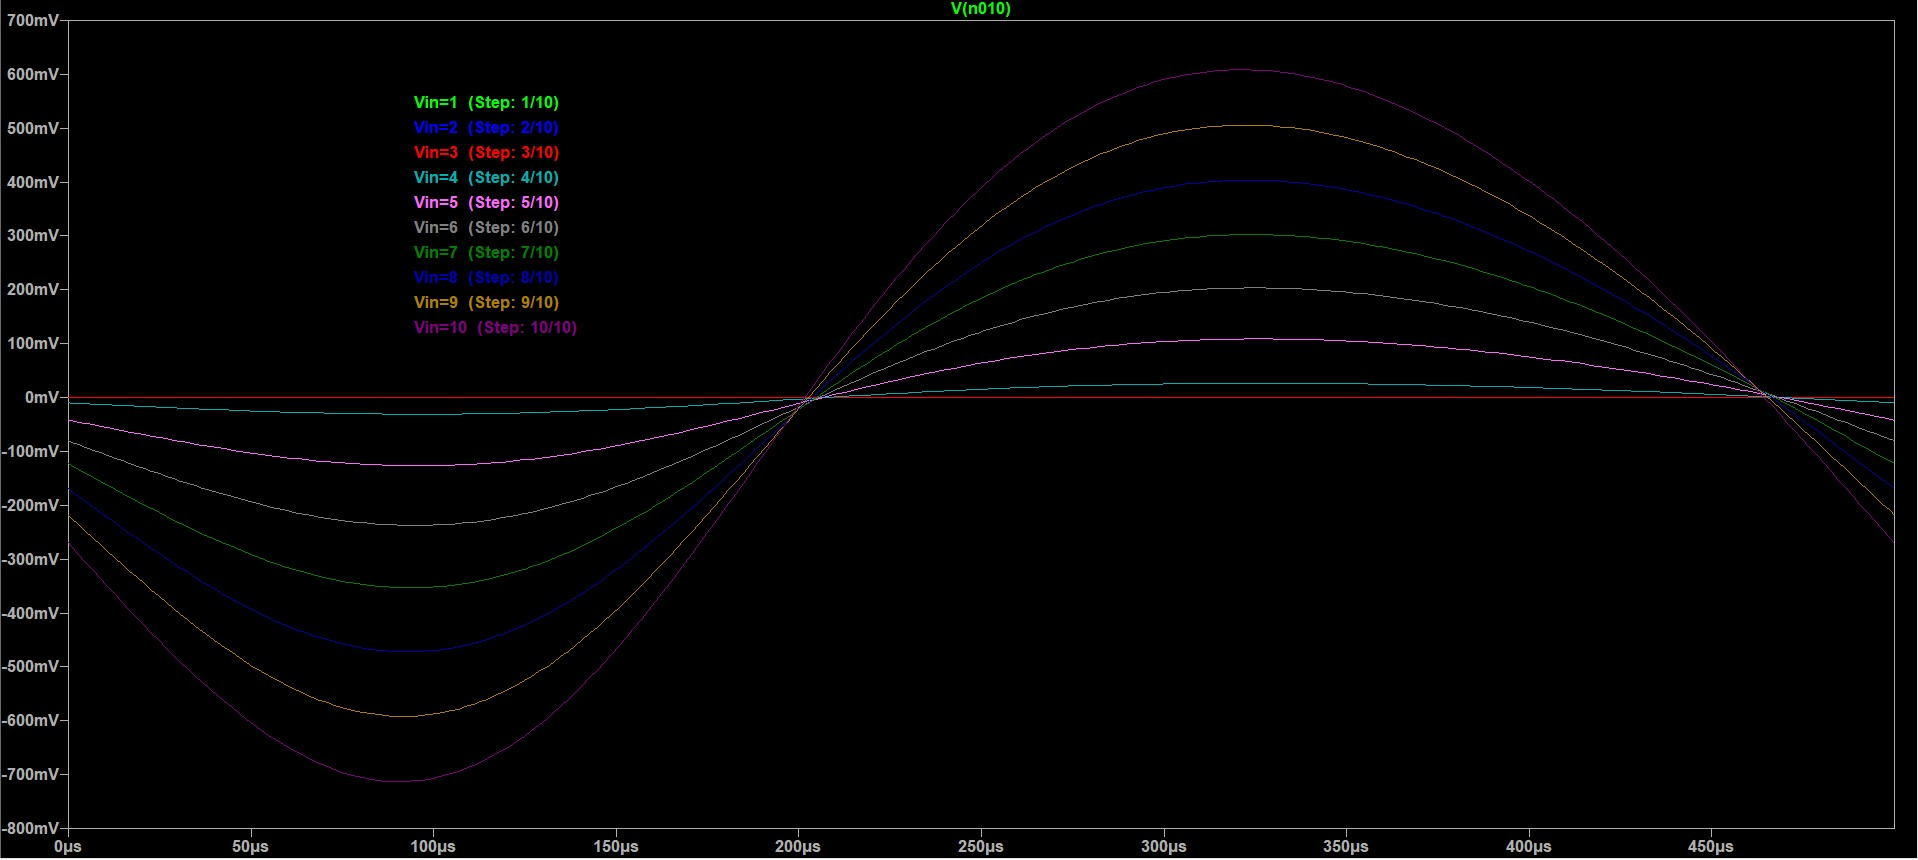
\includegraphics[width=0.75\linewidth]{Simu/voltajemuerteabajototal-salida.jpg}
    \caption{Comportamiento de la señal de salida ante la variación de la fuente de alimentación $V_{CC}$ (barrido hacia abajo).}
  \label{BarridoAbajo}
\end{figure}
\begin{figure}[H]
    \centering
    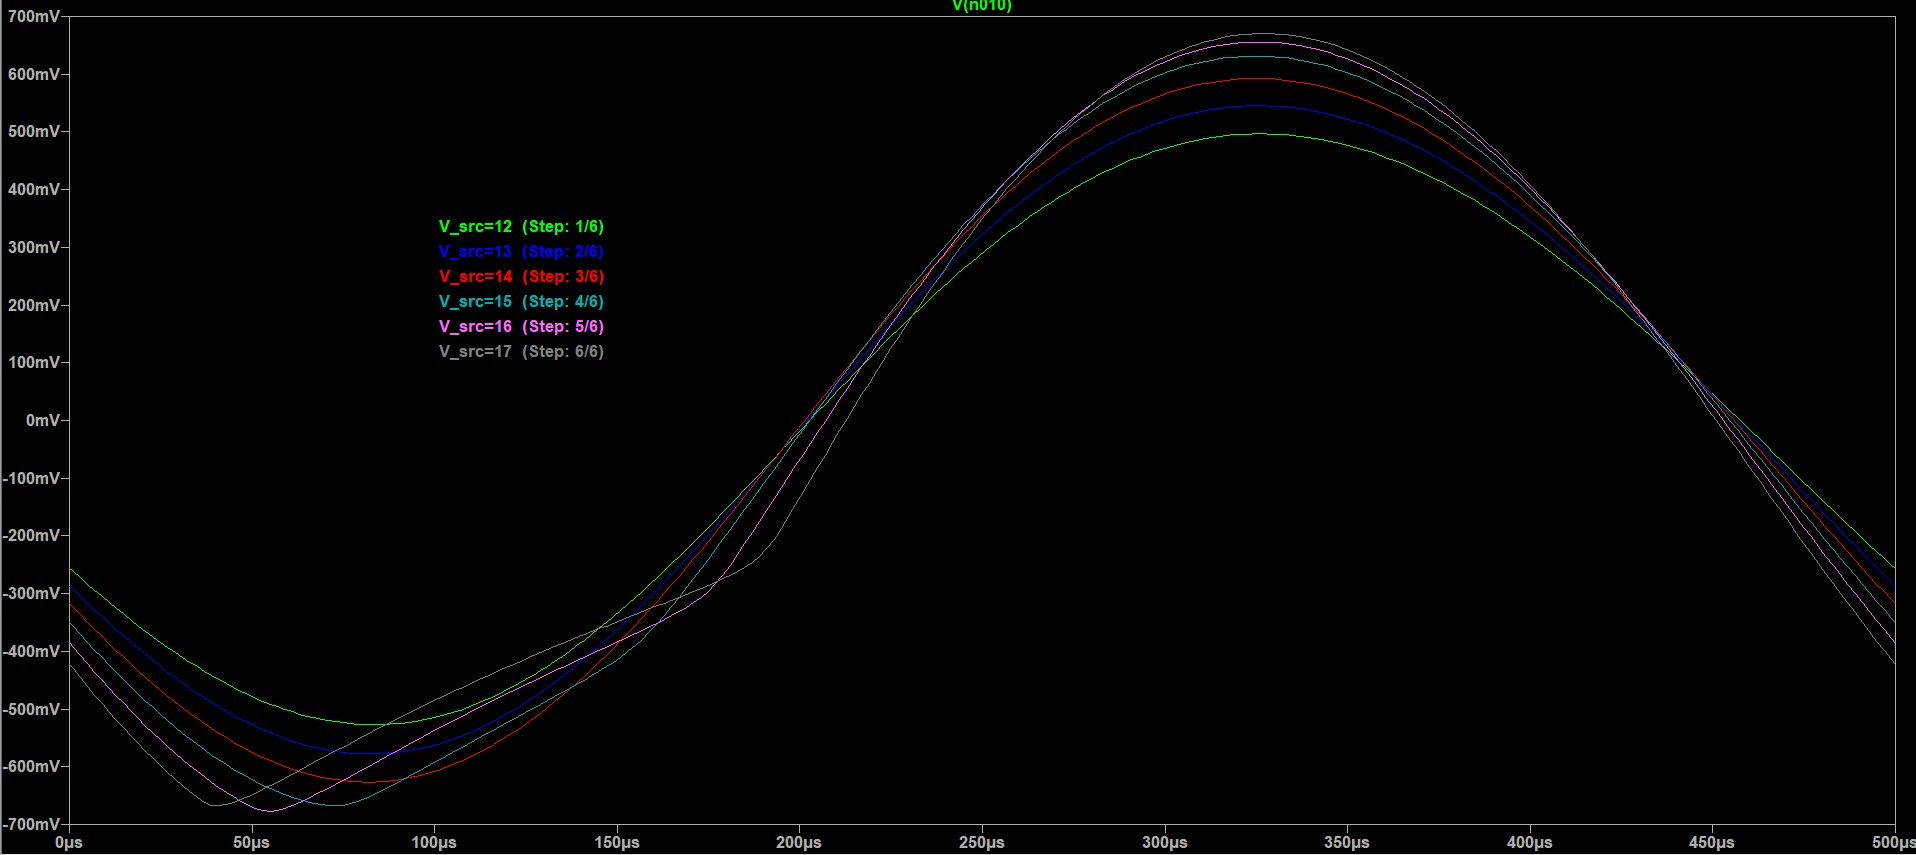
\includegraphics[width=0.75\linewidth]{Simu/voltajemuertearribatotal-salida.jpg}
    \caption{Comportamiento de la señal de salida ante la variación de la fuente de alimentación $V_{CC}$ (barrido hacia arriba).}
  \label{BarridoArriba}
\end{figure}

{\small\textbf{3- Límites de Operación por Variación de Carga ($R_L$)}}

%\paragraph{1.8.3. Límites de Operación por Variación de Carga ($R_L$)}
Se realizó un barrido sobre la impedancia de salida utilizando \texttt{.step param RL 4 16 2} para evaluar la capacidad de entrega de corriente del amplificador y determinar el rango de impedancias de carga sobre el cual se preserva la respuesta lineal sin recorte por corriente (\cref{GainRo}).

\begin{figure}[H]
    \centering
    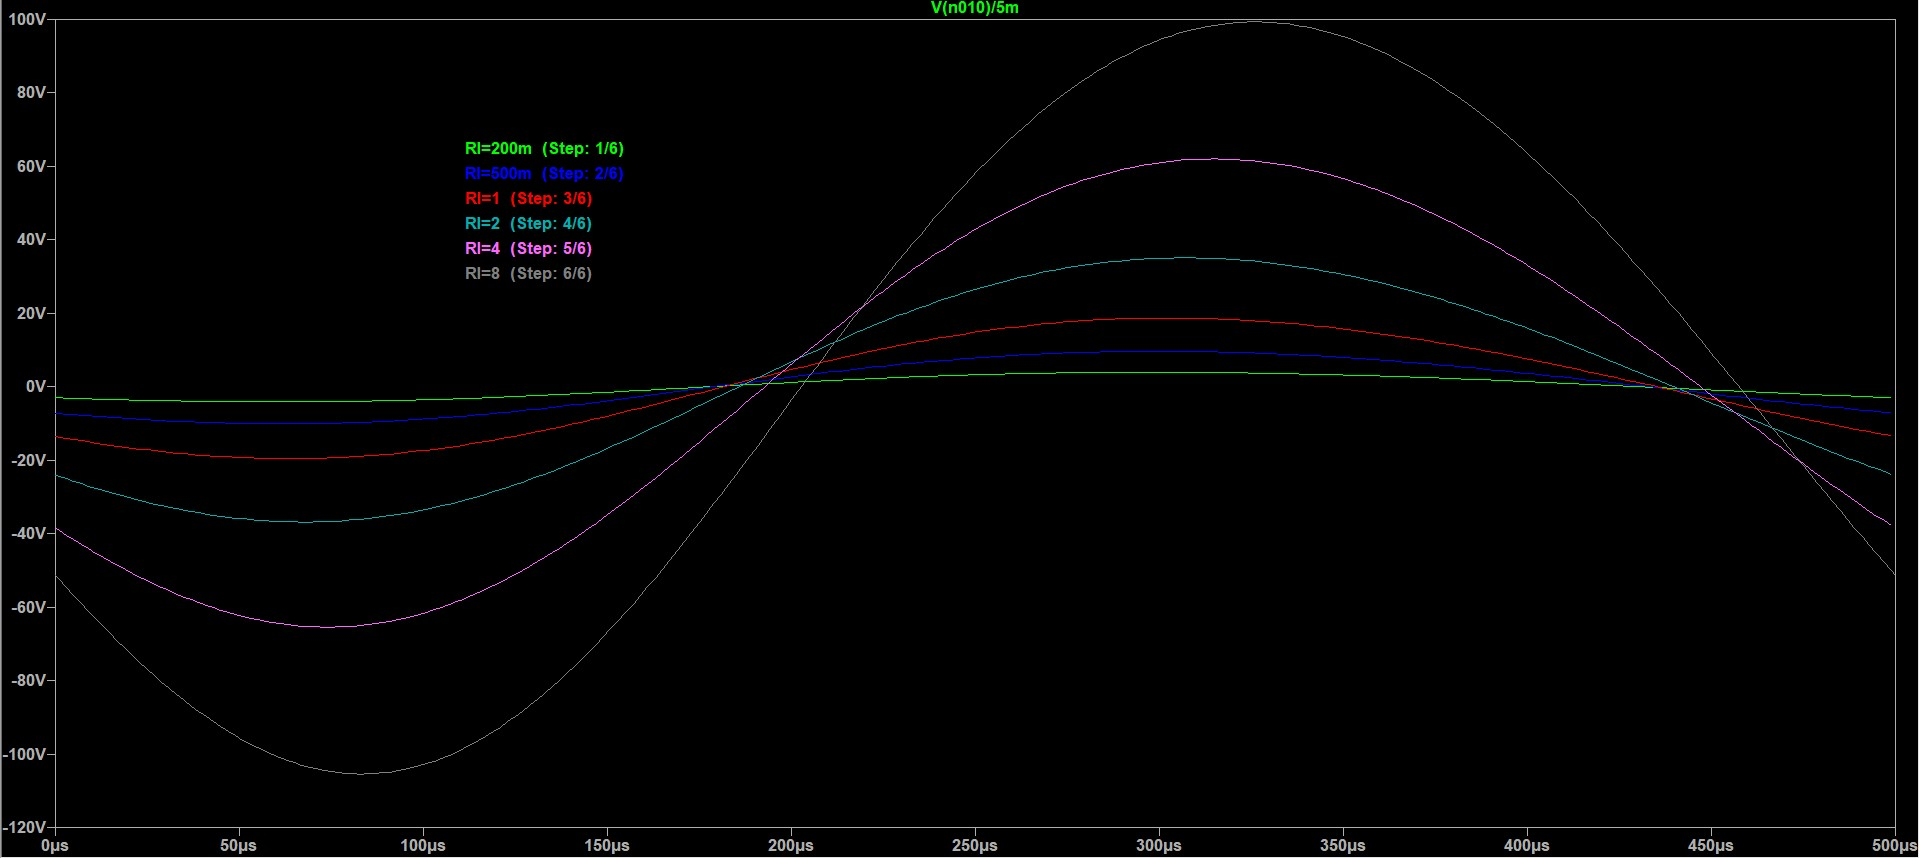
\includegraphics[width=0.75\linewidth]{Simu/RLMURTESALIDA.jpg}
    \caption{Ganancia frente a variaciones en la resistencia de carga $R_L$.}
  \label{GainRo}
\end{figure}

% =========================================================================
% APARTADO 2: ETAPA DARLINGTON
% =========================================================================
\subsubsection{Primera Etapa: Adaptador de Entrada Darlington ($Q_1$ - $Q_2$)}
%\section{2. Primera Etapa: Adaptador de Entrada Darlington ($Q_1$ - $Q_2$)}

\begin{figure}[H]
    \centering
    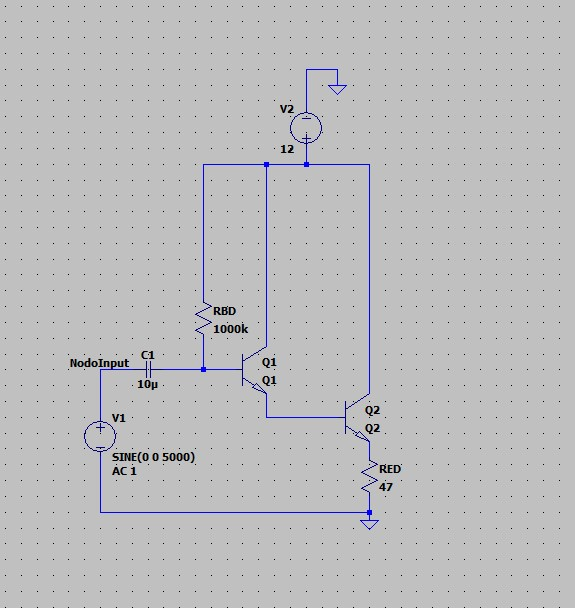
\includegraphics[width=0.45\linewidth]{Simu/Darlinton.jpg}
    \caption{Circuito esquemático de la etapa Darlington aislada.}
\end{figure}

\vspace{0.5em}
{\small\textbf{Polarización y Disipación de Potencia}}

%\subsubsection{2.1. Polarización y Disipación de Potencia}
Se determinó el punto estático mediante \texttt{.op}, evaluando las corrientes de colector y las tensiones $V_{CE}$ para calcular la disipación estática de $Q_1$ y $Q_2$.
\begin{verbatim}
.op
.meas DC VCE_Q1 PARAM V(vcc)-V(e1)
.meas DC IC_Q1 I(Q1)
.meas DC P_Q1 PARAM VCE_Q1*IC_Q1
\end{verbatim}

\vspace{0.5em}
{\small\textbf{Medición de Impedancias de la Etapa Darlington ($Z_{in1}$ y $Z_{out1}$)}}

%\subsubsection{2.2. Medición de Impedancias de la Etapa Darlington ($Z_{in1}$ y $Z_{out1}$)}
La impedancia de entrada $Z_{in1}$ se midió inyectando señal desde la fuente de entrada $V_1$. Para la impedancia de salida $Z_{out1}$, se aisló la etapa, se pasivó la entrada y se colocó una fuente de prueba $I_{test}$ en el emisor de $Q_2$.

\paragraph{Impedancia de Entrada ($Z_{in1}$)} 
Se puede ver en (\cref{SimuZin1}).
\begin{figure}[H]
    \centering
    \begin{minipage}{0.48\textwidth}
        \centering
        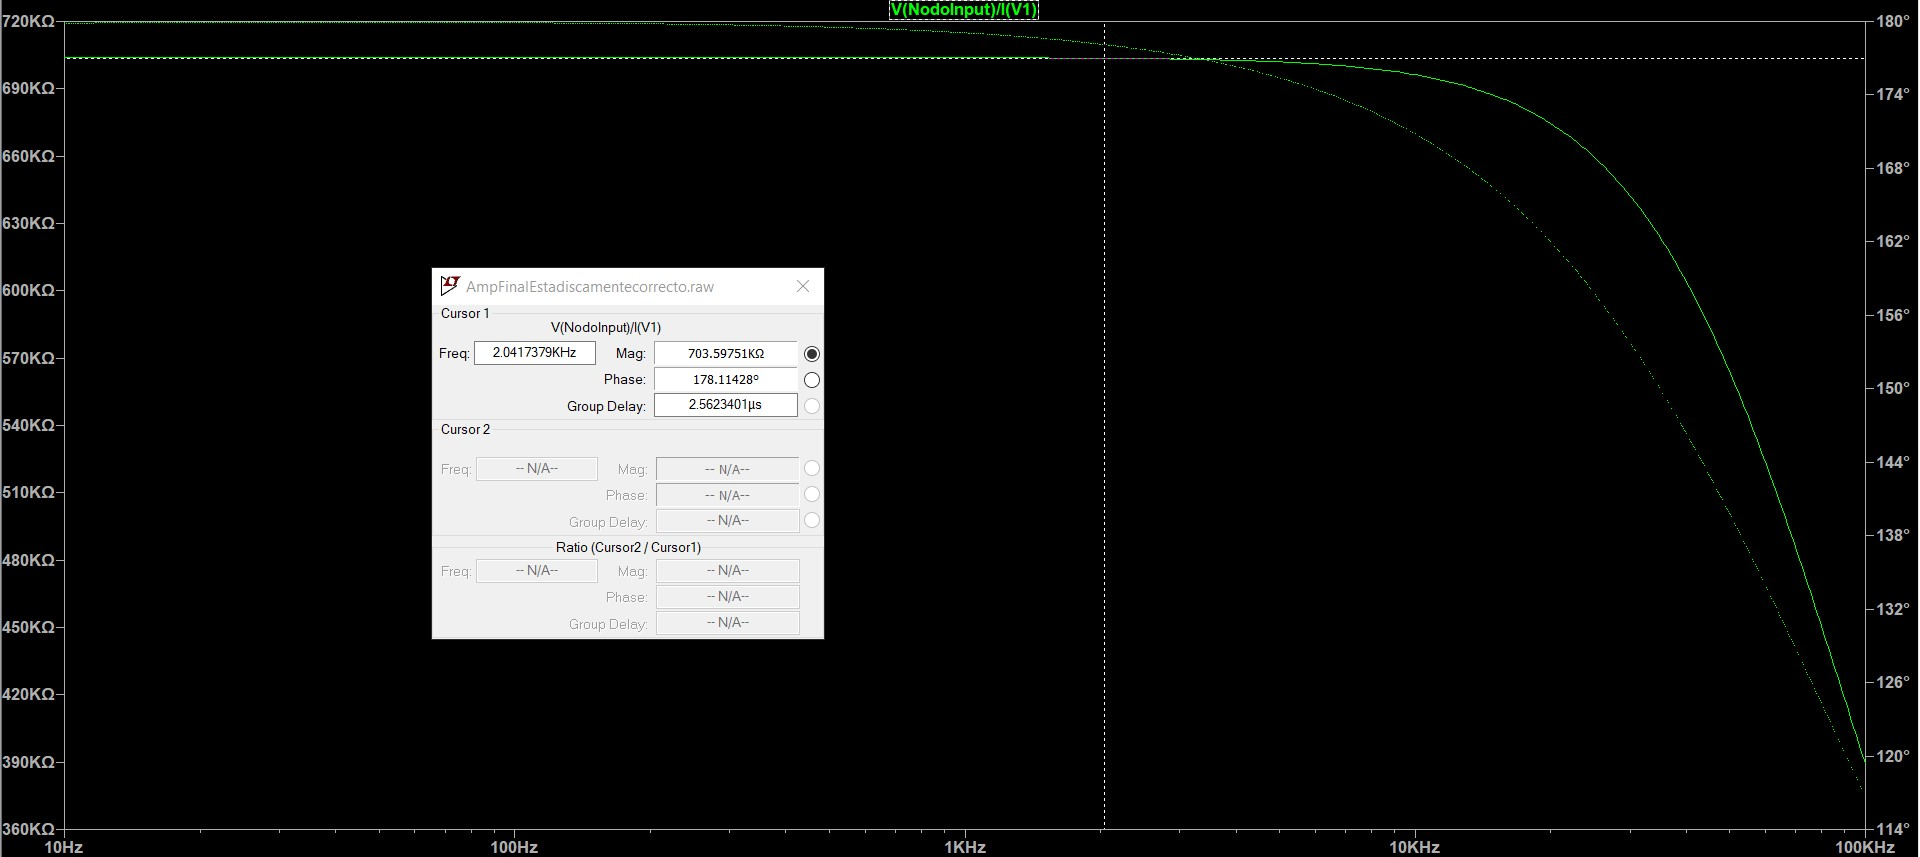
\includegraphics[width=\linewidth]{Simu/ImpedanciaIN_Darlinton.jpg}
        \caption{Curva de respuesta $Z_{in1}$.}
    \label{SimuZin1}
    \end{minipage}
\end{figure}

\paragraph{Impedancia de Salida ($Z_{out1}$)} 
Se puede ver en (\cref{SimuZout1}).
\begin{figure}[H]
    \centering
    \begin{minipage}{0.48\textwidth}
        \centering
        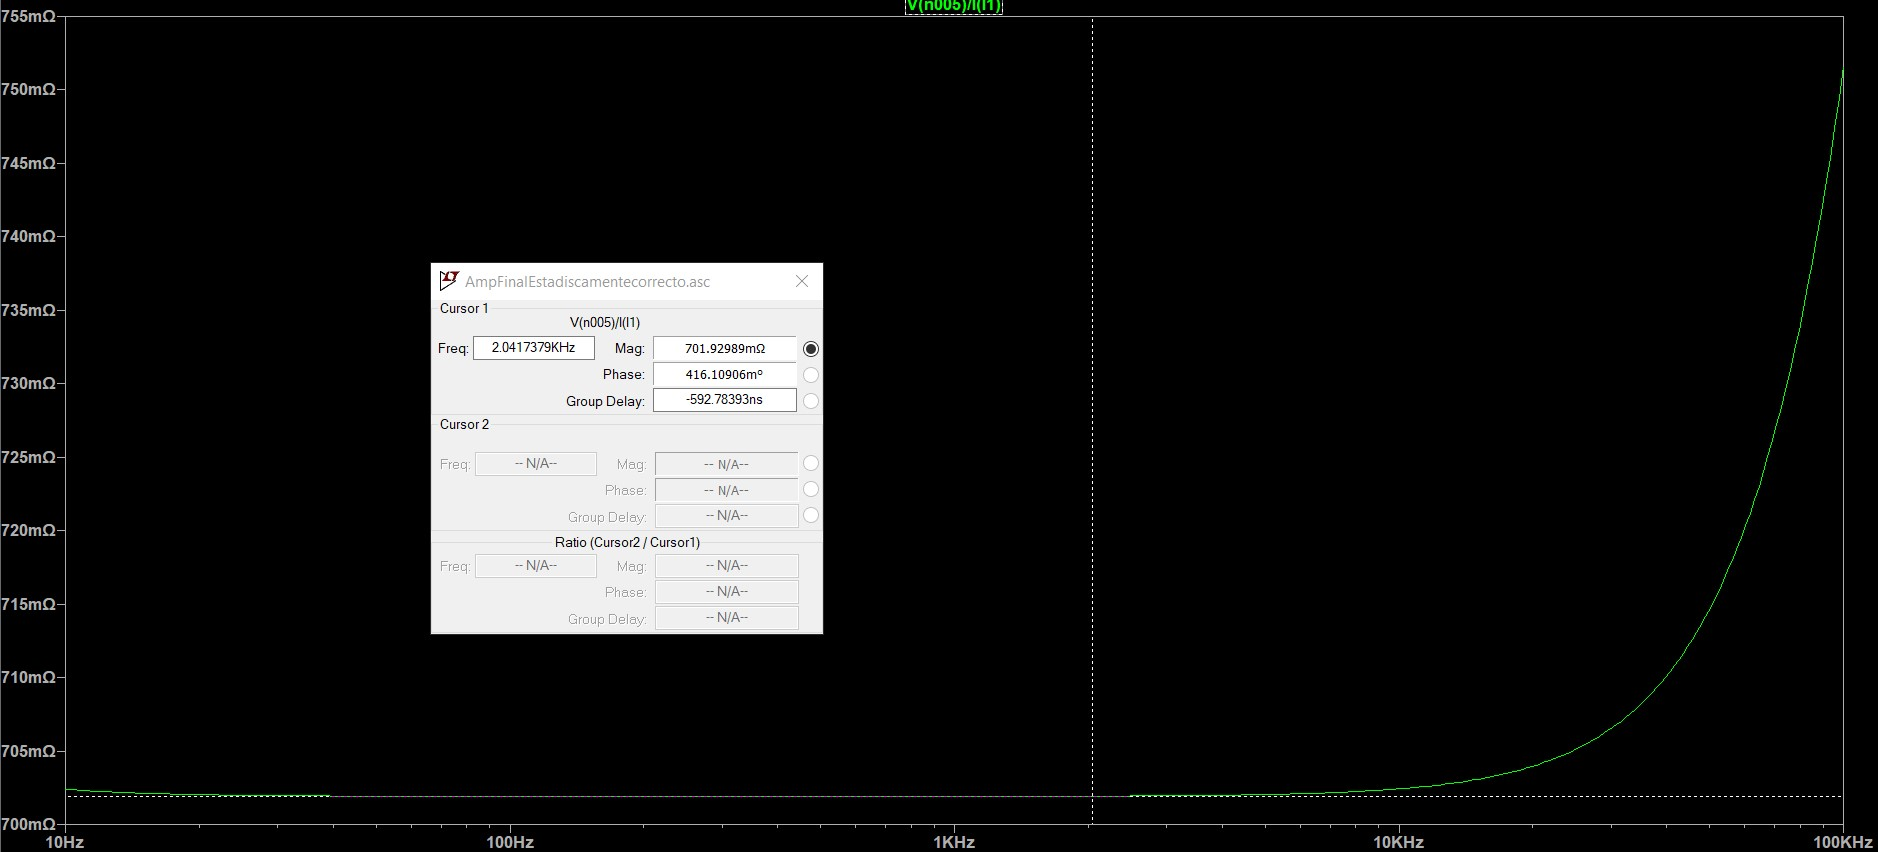
\includegraphics[width=\linewidth]{Simu/ImpedanciaOUT_Darlinton.jpg}
        \caption{Curva de respuesta de $Z_{out1}$.}
  \label{SimuZout1}
    \end{minipage}
\end{figure}

\vspace{0.5em}
{\small\textbf{Respuesta en Frecuencia, Temporal, Ruido y Linealidad}}

%\subsubsection{2.3. Respuesta en Frecuencia, Temporal, Ruido y Linealidad}
Se caracterizó la respuesta frecuencial mediante barrido \texttt{.ac}, la excursión temporal con \texttt{.tran}, la PSD de ruido a la salida de la etapa con \texttt{.noise} y la respuesta dinámica X-Y con \texttt{.step param A\_in} (\cref{SimuBW}, \cref{SimuVtemp}, \cref{SimuPSDDar}, \cref{SimuLinDar}).

\begin{figure}[H]
    \centering
    \begin{minipage}{0.48\textwidth}
        \centering
        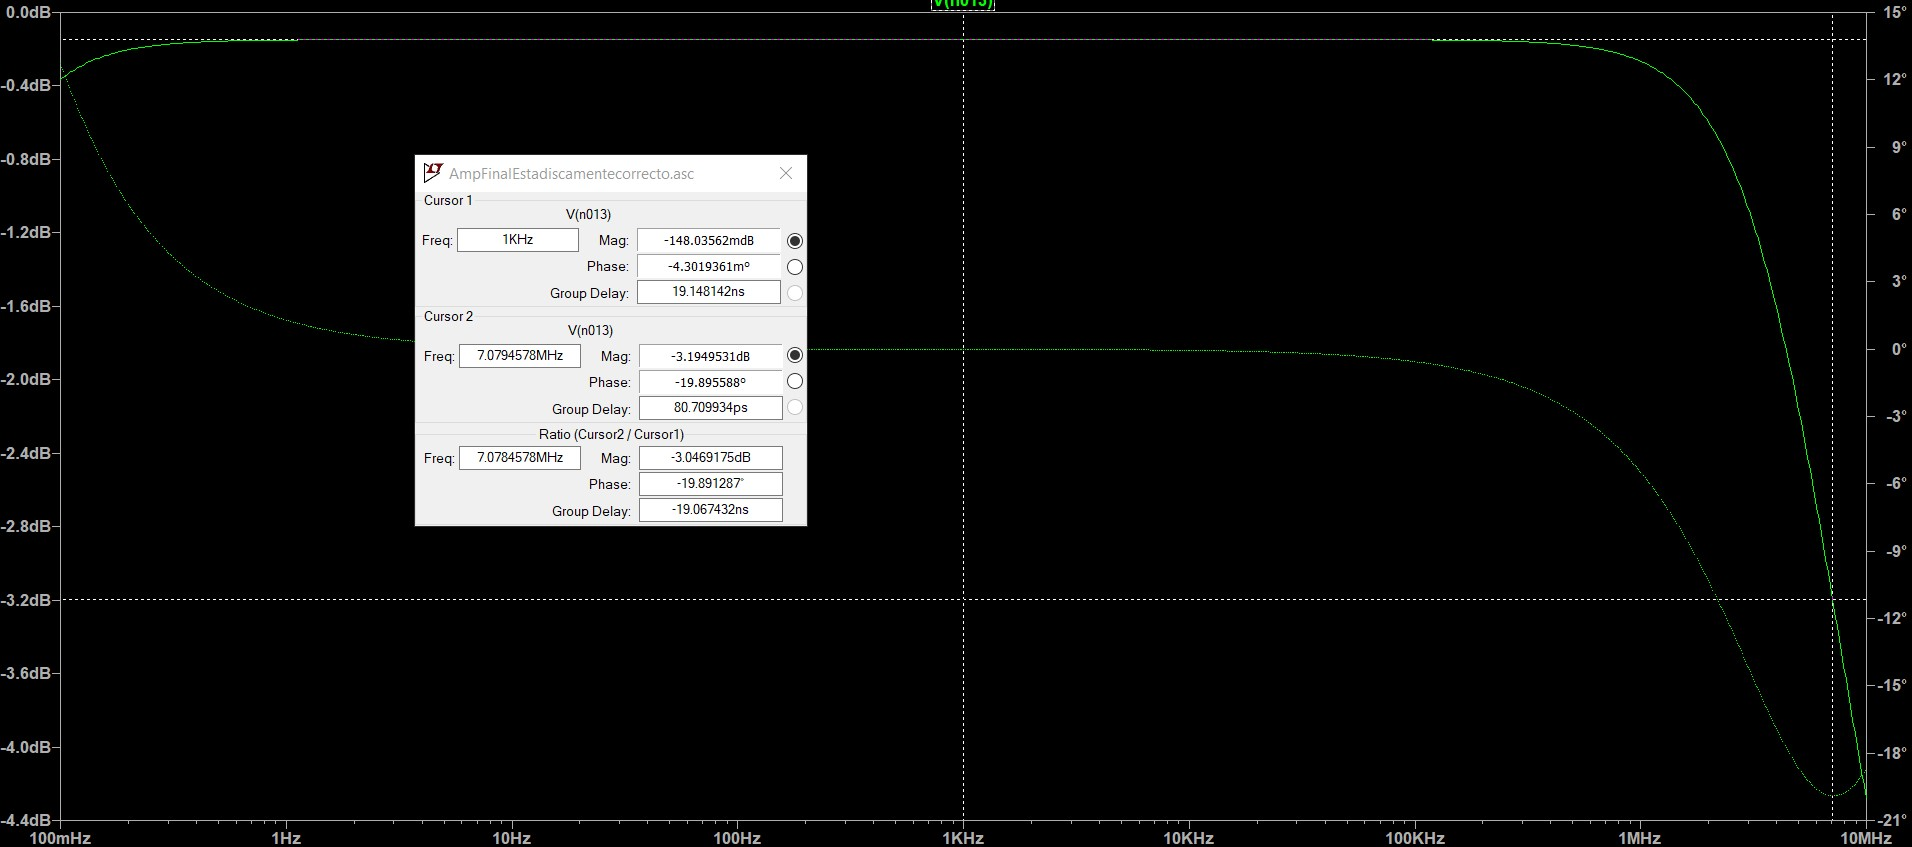
\includegraphics[width=\linewidth]{Simu/BW-DARLINTONG-DB.jpg}
        \caption{Respuesta AC (Ancho de banda).}
      \label{SimuBW}
    \end{minipage}\hfill
    \begin{minipage}{0.48\textwidth}
        \centering
        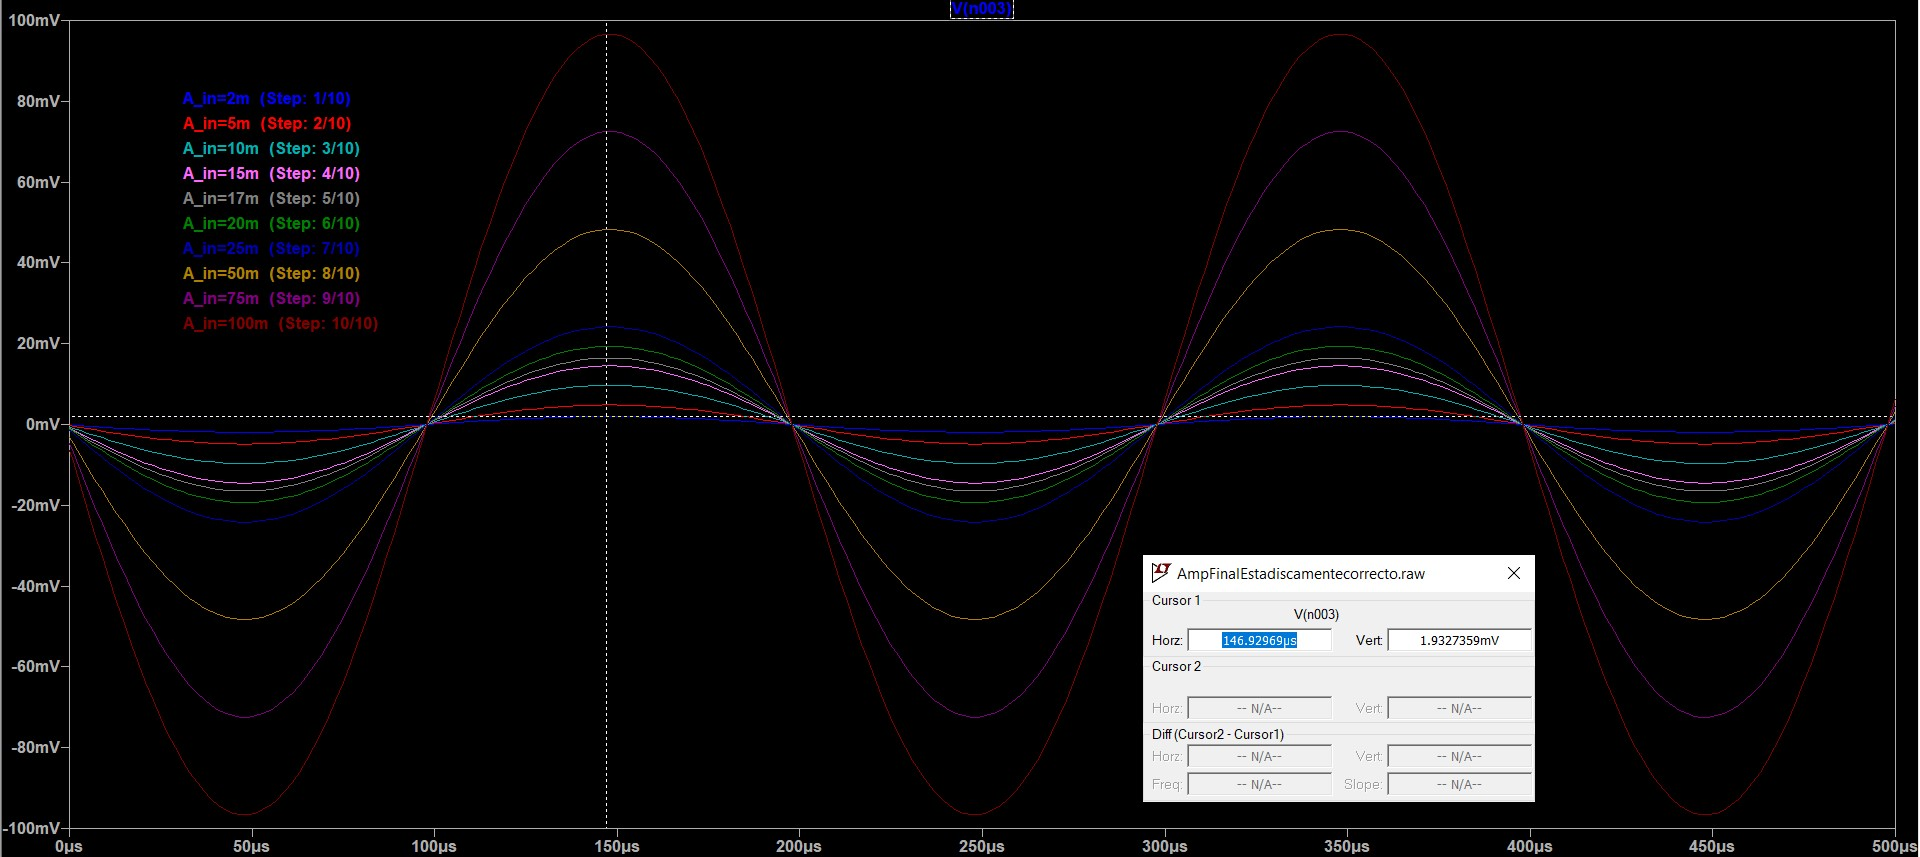
\includegraphics[width=\linewidth]{Simu/Voutppdarlin.jpg}
        \caption{Tensión temporal pico a pico.}
      \label{SimuVtemp}
    \end{minipage}
\end{figure}

\begin{figure}[H]
    \centering
    \begin{minipage}{0.48\textwidth}
        \centering
        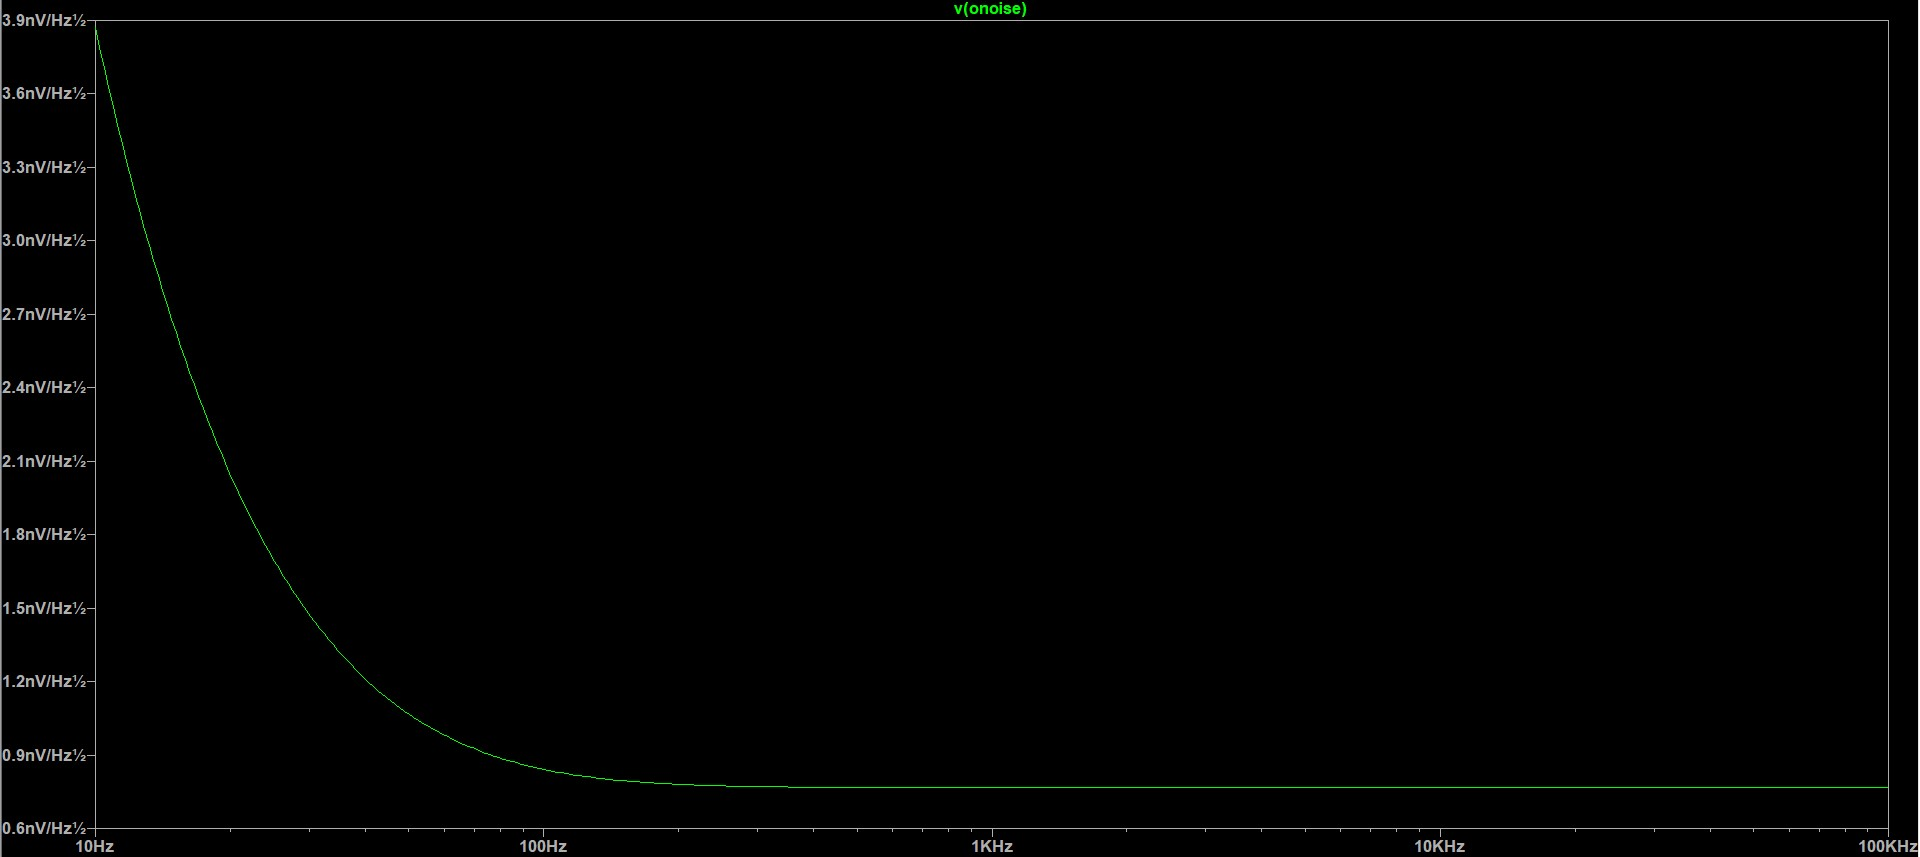
\includegraphics[width=\linewidth]{Simu/Noise-dar.jpg}
        \caption{PSD de Ruido - Darlington.}
      \label{SimuPSDDar}
    \end{minipage}\hfill
    \begin{minipage}{0.48\textwidth}
        \centering
        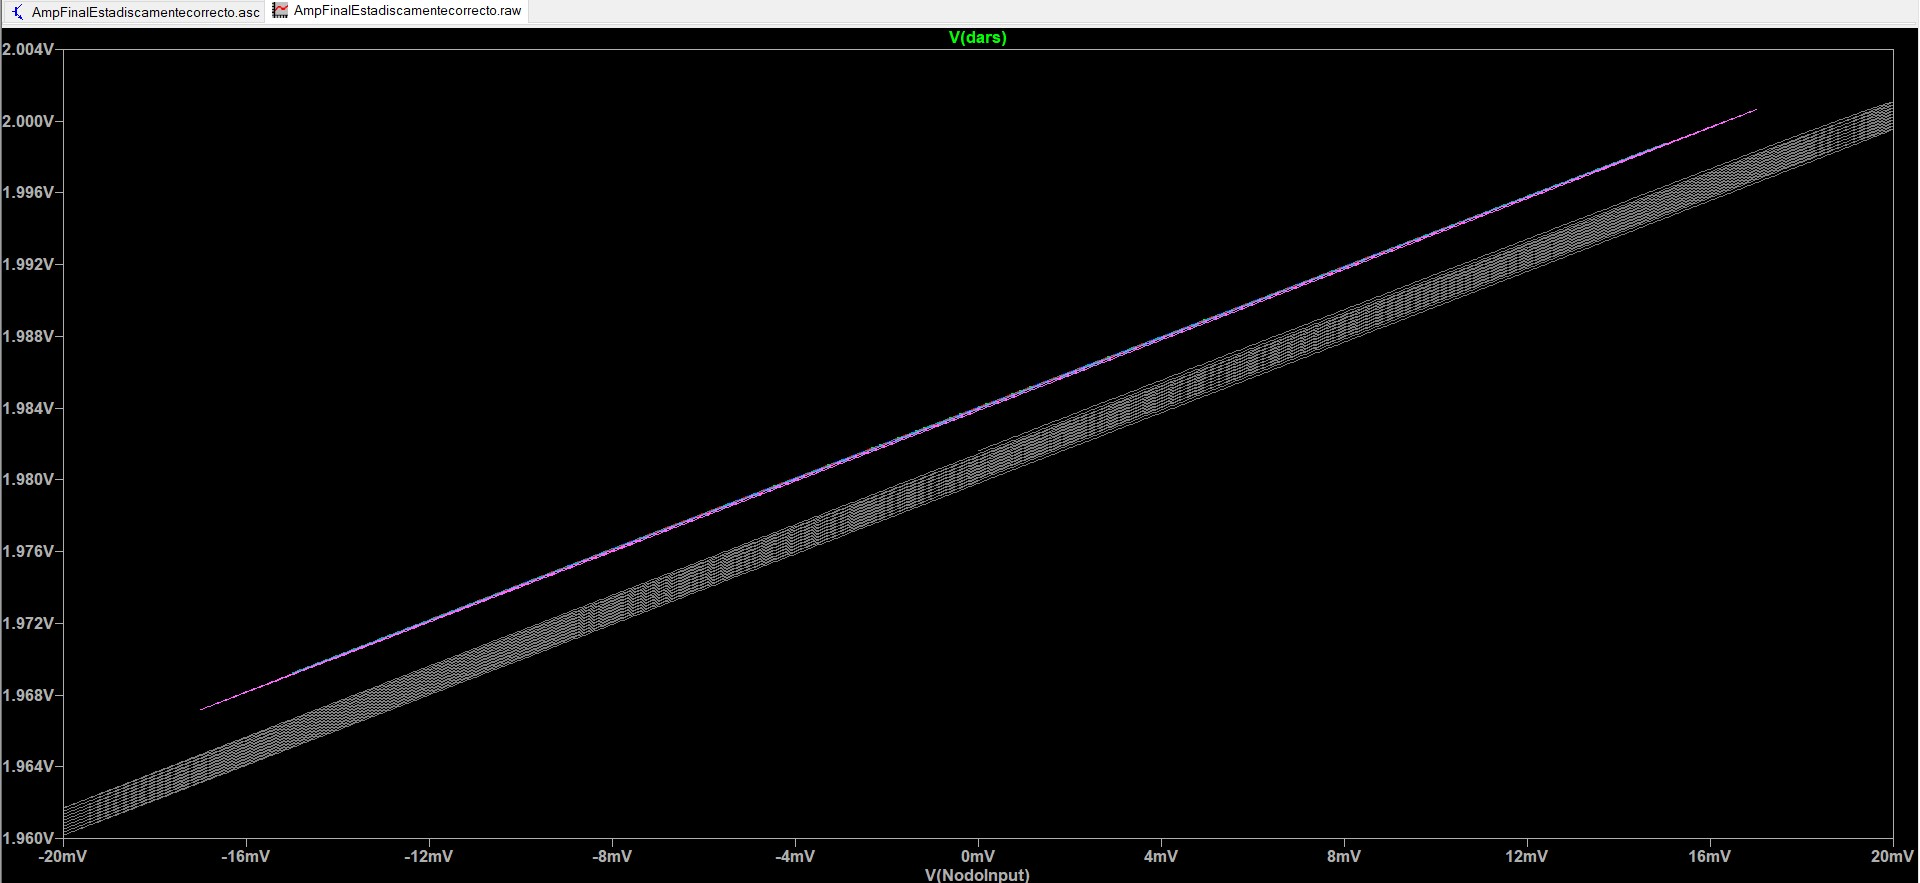
\includegraphics[width=\linewidth]{Simu/LINEALIDAD-DAR.jpg}
        \caption{Evaluación de Linealidad.}
      \label{SimuLinDar}
    \end{minipage}
\end{figure}

% =========================================================================
% APARTADO 3: ETAPA EMISOR COMUN
% =========================================================================

\subsubsection{Segunda Etapa: Ganancia de Tensión en Emisor Común ($Q_3$)}
%\section{3. Segunda Etapa: Ganancia de Tensión en Emisor Común ($Q_3$)}

\begin{figure}[H]
    \centering
    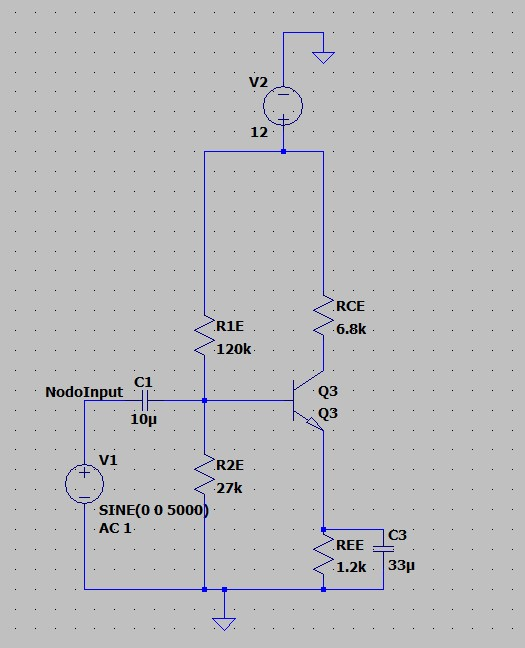
\includegraphics[width=0.45\linewidth]{Simu/Emisor_Aislado.jpg}
    \caption{Circuito esquemático de la etapa de Emisor Común aislada.}
\end{figure}

\vspace{0.5em}
{\small\textbf{Polarización y Disipación de Potencia}}

%\subsubsection{3.1. Polarización y Disipación de Potencia}
Se utilizó la directiva \texttt{.op} para registrar la corriente de colector $I_{C3}$ y la tensión $V_{CE3}$, asegurando la ubicación del punto de trabajo en la región activa.
\begin{verbatim}
.op
.meas DC VCE_Q3 PARAM V(NodoColector_Q3)-V(NodoEmisor_Q3)
.meas DC IC_Q3 I(Q3)
\end{verbatim}

\vspace{0.5em}
{\small\textbf{Medición de Impedancias de la Etapa Emisor Común ($Z_{in2}$ y $Z_{out2}$)}}

%\subsubsection{3.2. Medición de Impedancias de la Etapa Emisor Común ($Z_{in2}$ y $Z_{out2}$)}
Para la impedancia de entrada $Z_{in2}$, se aplicó tensión en la base de $Q_3$. Para la impedancia de salida $Z_{out2}$, se desacopló la carga/tercera etapa, se pasivó la entrada y se aplicó una fuente de prueba en el colector.

\paragraph{Impedancia de Entrada ($Z_{in2}$)}
Se puede ver en (\cref{SimuZin2}).
\begin{figure}[H]
    \centering
    \begin{minipage}{0.48\textwidth}
        \centering
        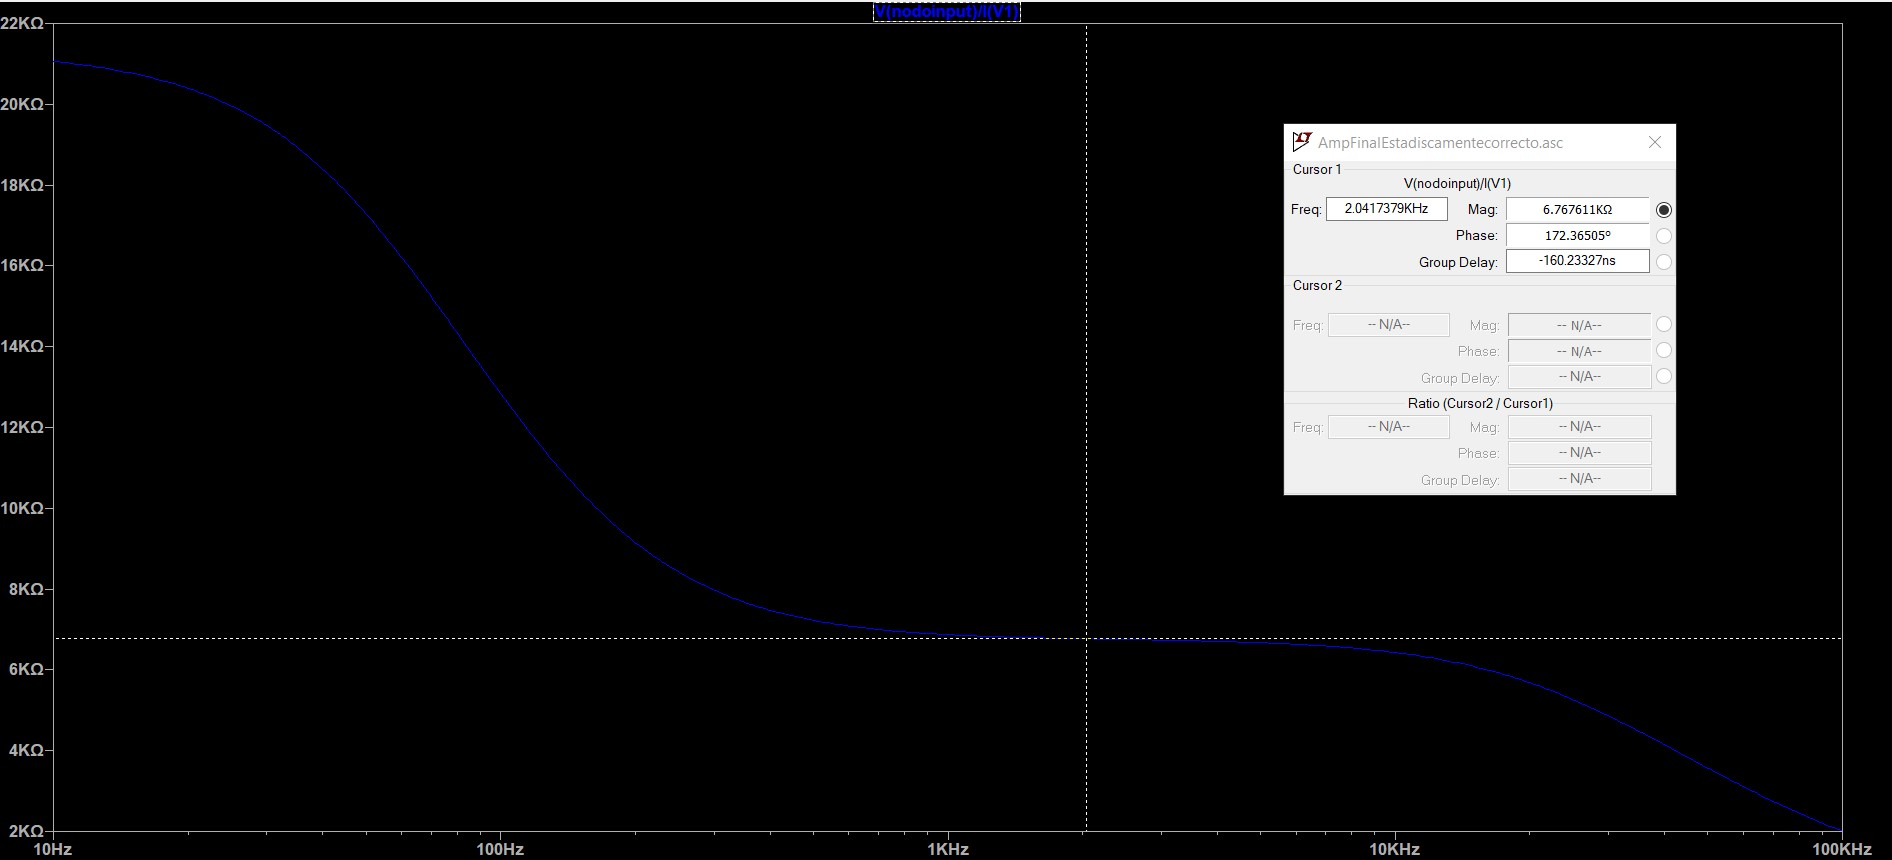
\includegraphics[width=\linewidth]{Simu/Emisor_ZIN.jpg}
        \caption{Curva de respuesta de $Z_{in2}$.}
      \label{SimuZin2}
    \end{minipage}
\end{figure}

\paragraph{Impedancia de Salida ($Z_{out2}$)}
Se puede ver en (\cref{SimuZout2}).
\begin{figure}[H]
    \centering
    \begin{minipage}{0.48\textwidth}
        \centering
        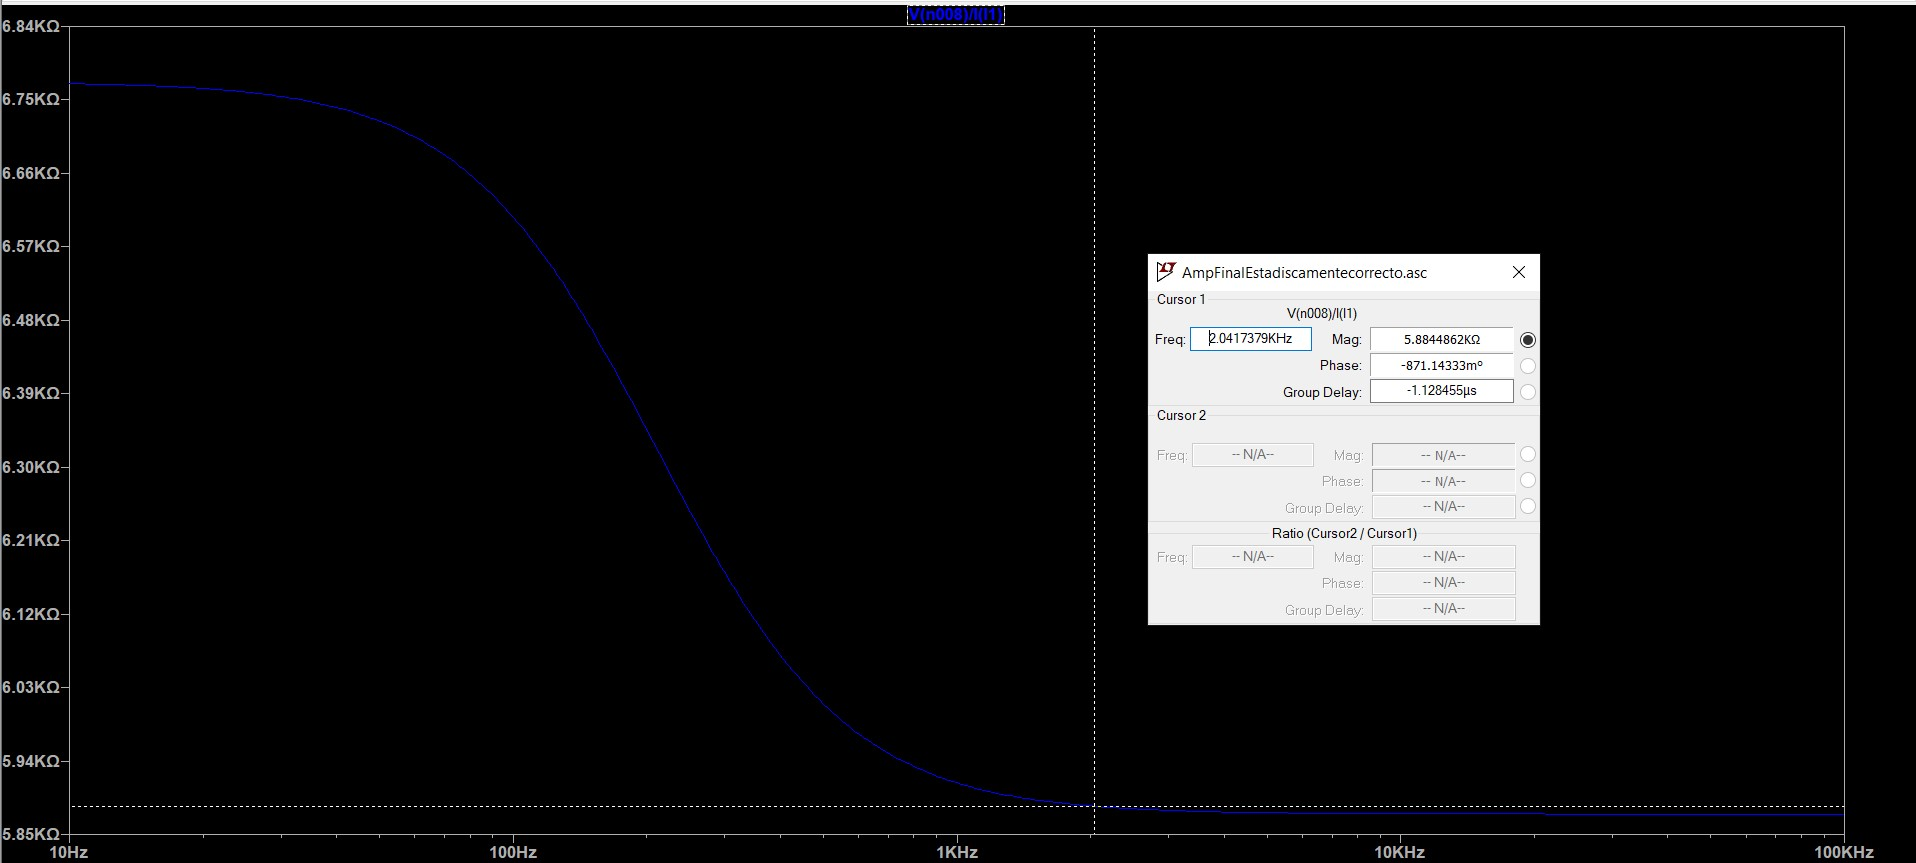
\includegraphics[width=\linewidth]{Simu/Emisor_Zout.jpg}
        \caption{Curva de respuesta de $Z_{out2}$.}
      \label{SimuZout2}
    \end{minipage}
\end{figure}

\vspace{0.5em}
{\small\textbf{Respuesta en Frecuencia, Temporal, Ruido, Límites de $V_{CC}$ y Linealidad}}

%\subsubsection{3.3. Respuesta en Frecuencia, Temporal, Ruido, Límites de $V_{CC}$ y Linealidad}
Se analizó la ganancia de tensión y respuesta frecuencial (\texttt{.ac}), la respuesta temporal (\texttt{.tran}), la PSD de ruido (\texttt{.noise}), el límite por variación de la fuente $V_{CC}$ y la pérdida de linealidad mediante la transferencia $V_{out}$ vs $V_{in}$ (\cref{SimuBWEC}, \cref{SimuETEC}, \cref{SimuPSDEC}, \cref{SimuVarVccEC}, \cref{SimuLinEC}).

\begin{figure}[H]
    \centering
    \begin{minipage}{0.48\textwidth}
        \centering
        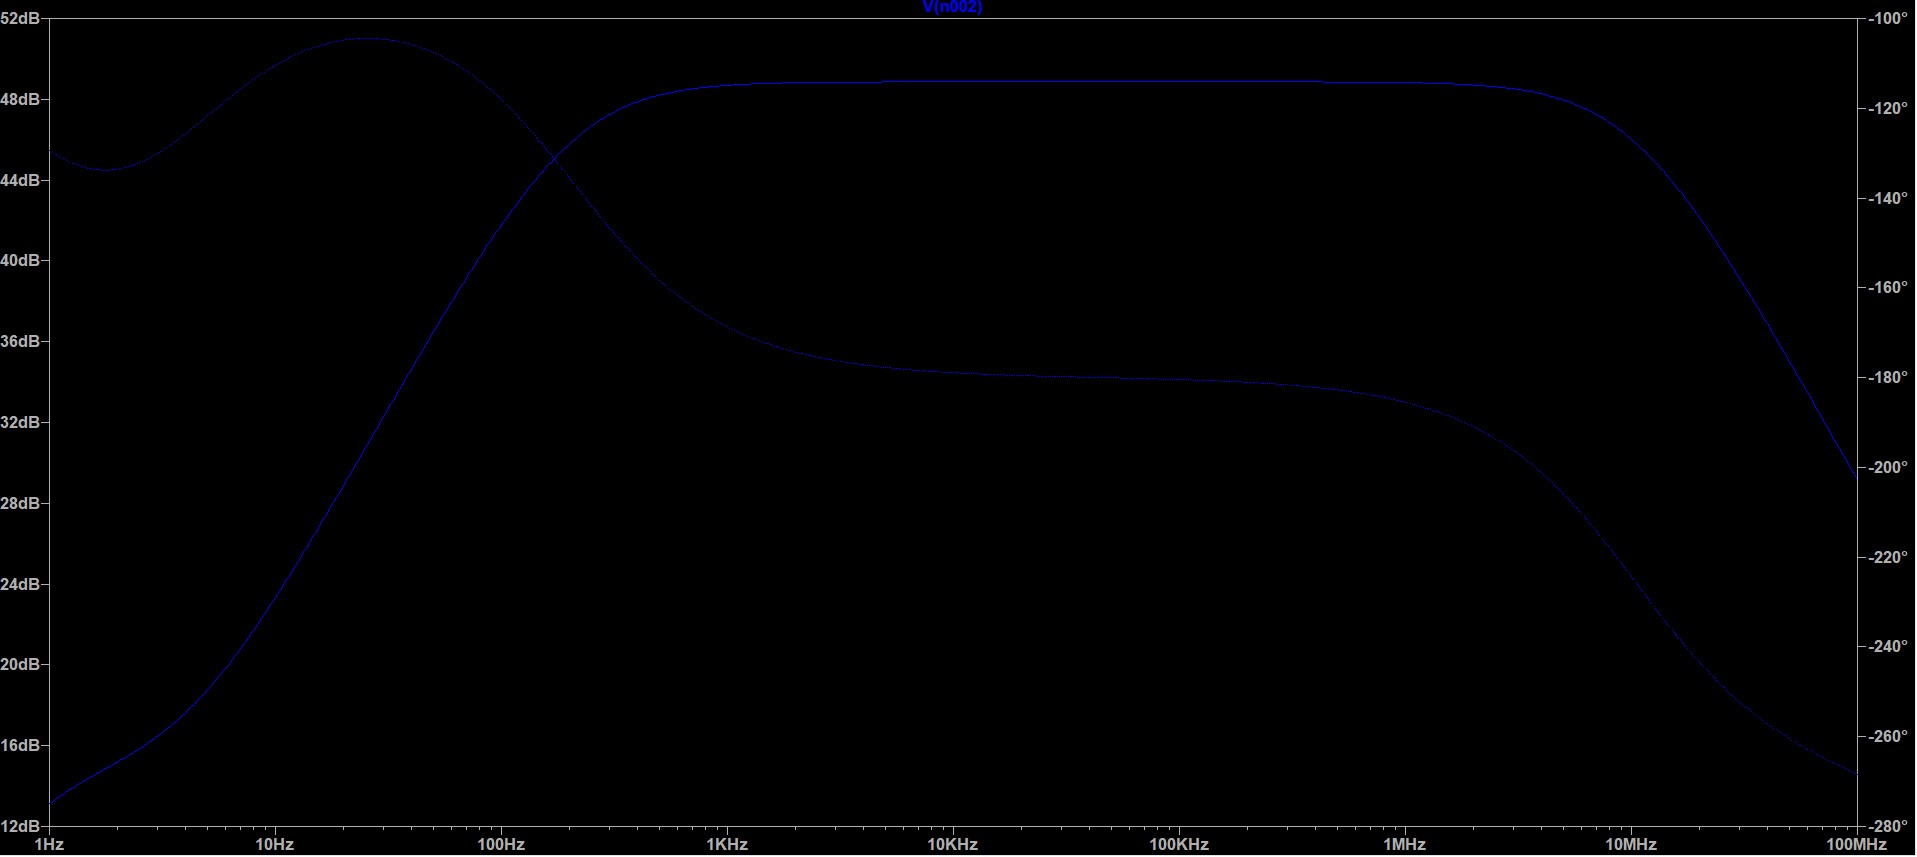
\includegraphics[width=\linewidth]{Simu/BW-EMISOR.jpg}
        \caption{Ancho de banda - Emisor Común.}
      \label{SimuBWEC}
    \end{minipage}\hfill
    \begin{minipage}{0.48\textwidth}
        \centering
        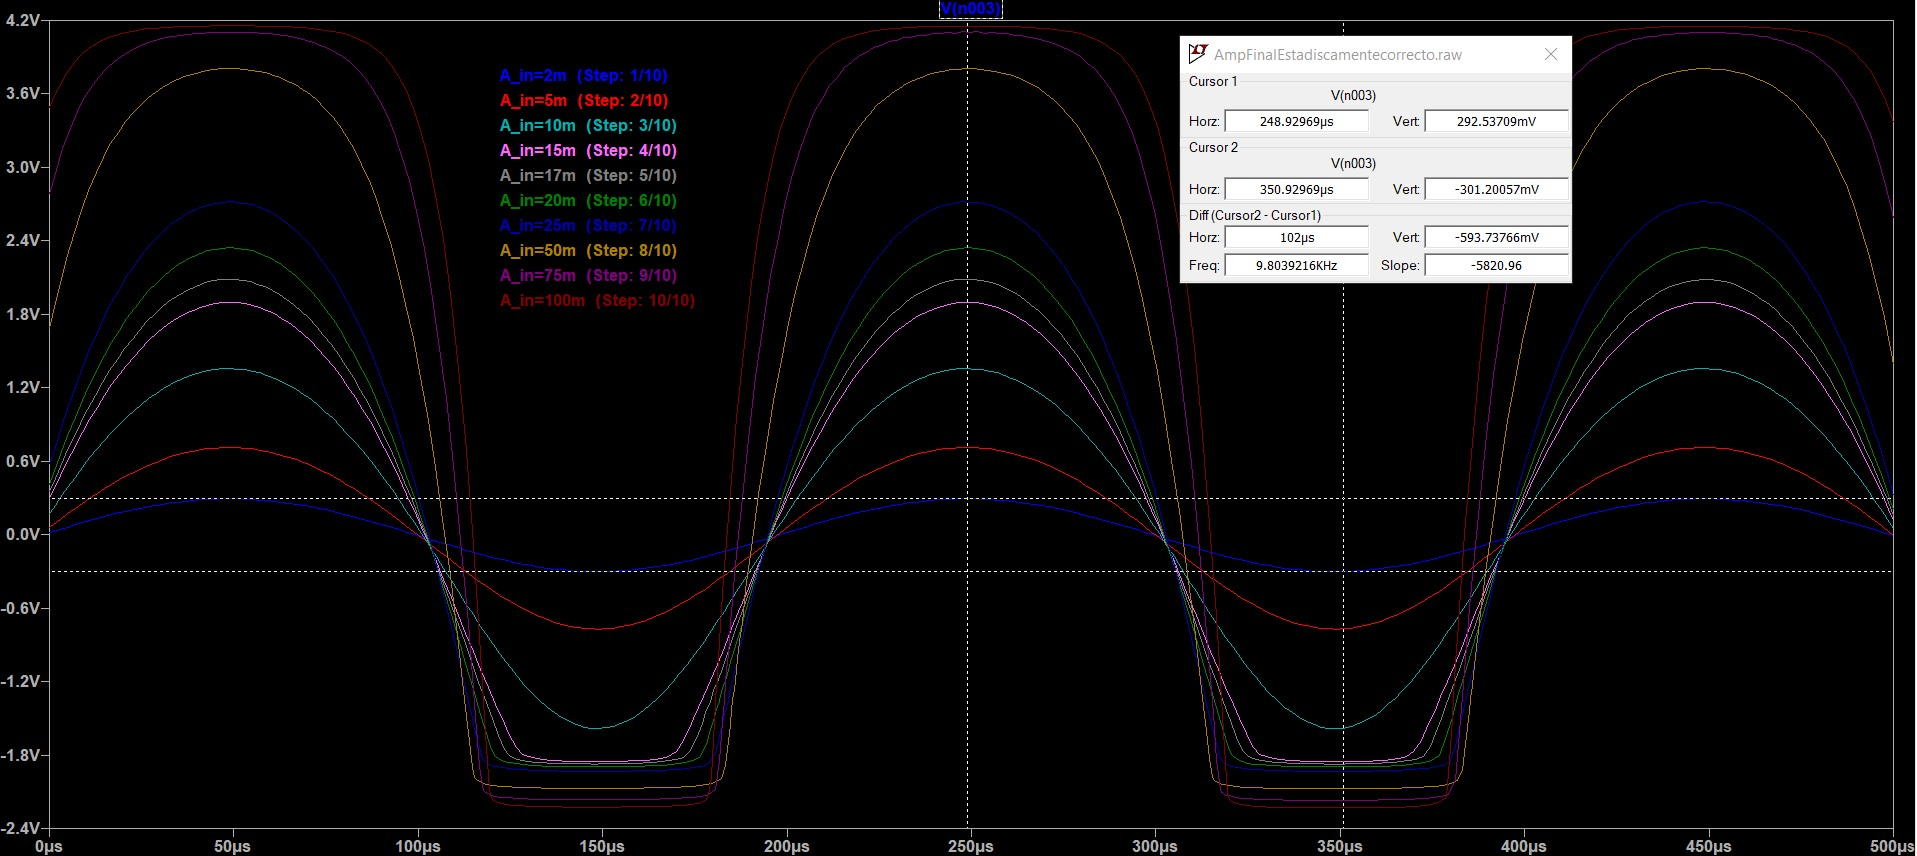
\includegraphics[width=\linewidth]{Simu/VPP-EMISOR.jpg}
        \caption{Excursión temporal $V_{pp}$.}
      \label{SimuETEC}
    \end{minipage}
\end{figure}

\begin{figure}[H]
    \centering
    \begin{minipage}{0.48\textwidth}
        \centering
        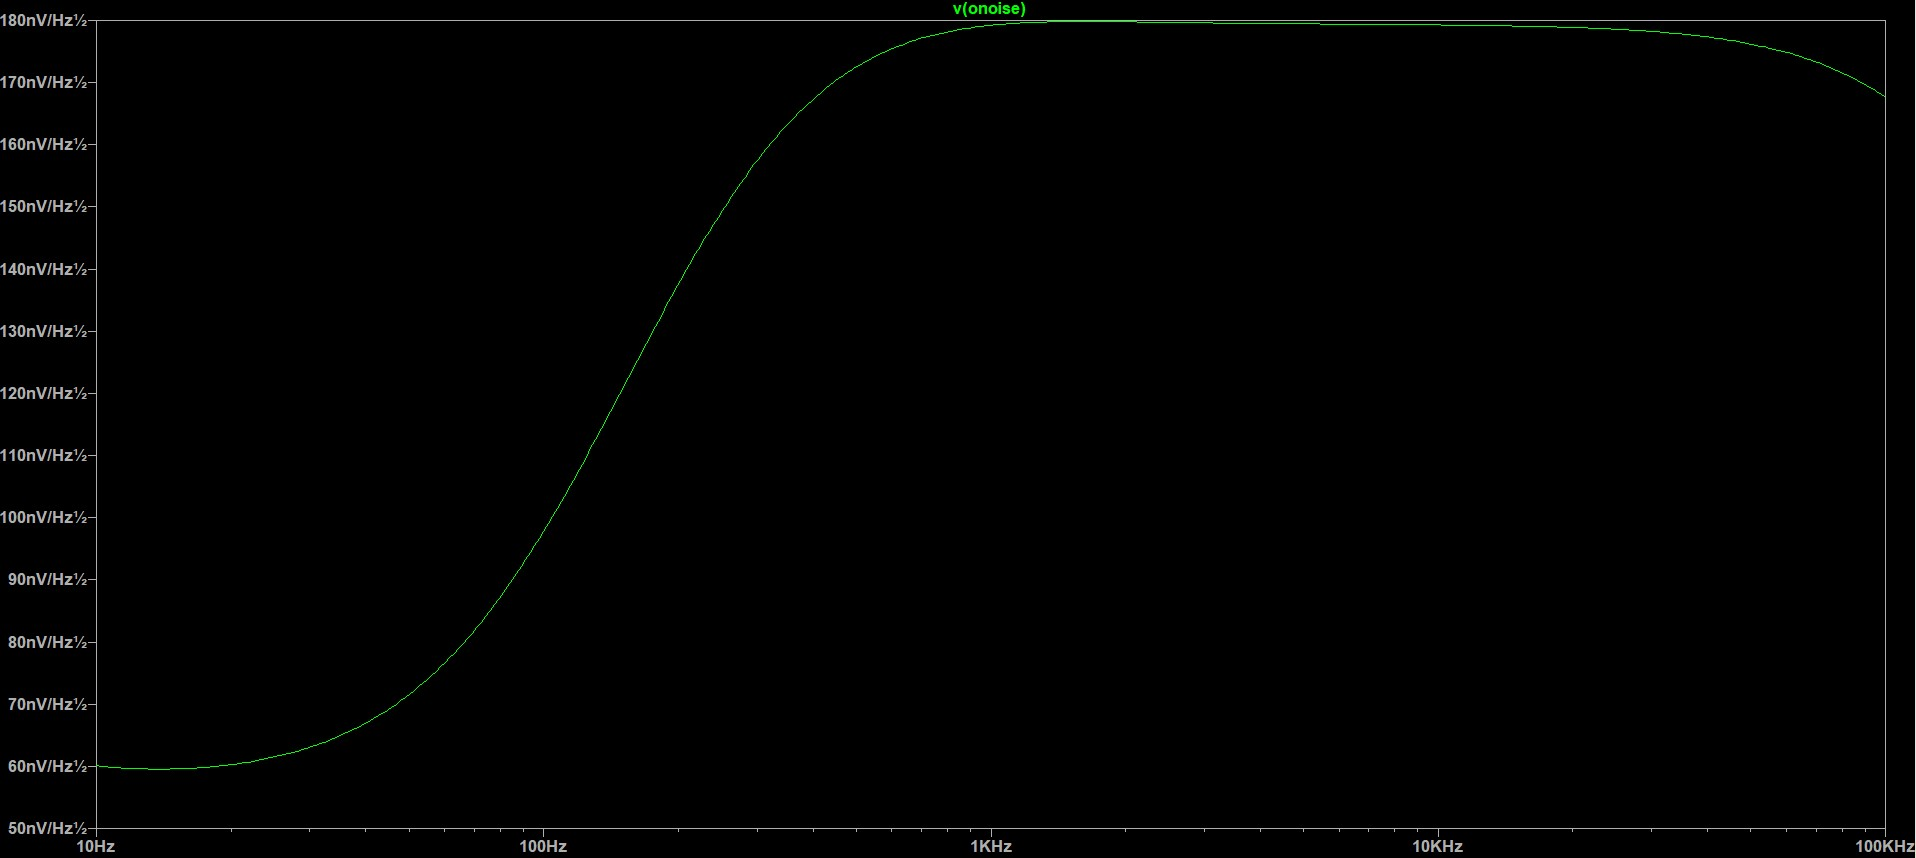
\includegraphics[width=\linewidth]{Simu/NOISE-EM.jpg}
        \caption{PSD de Ruido - Emisor Común.}
      \label{SimuPSDEC}
    \end{minipage}\hfill
    \begin{minipage}{0.48\textwidth}
        \centering
        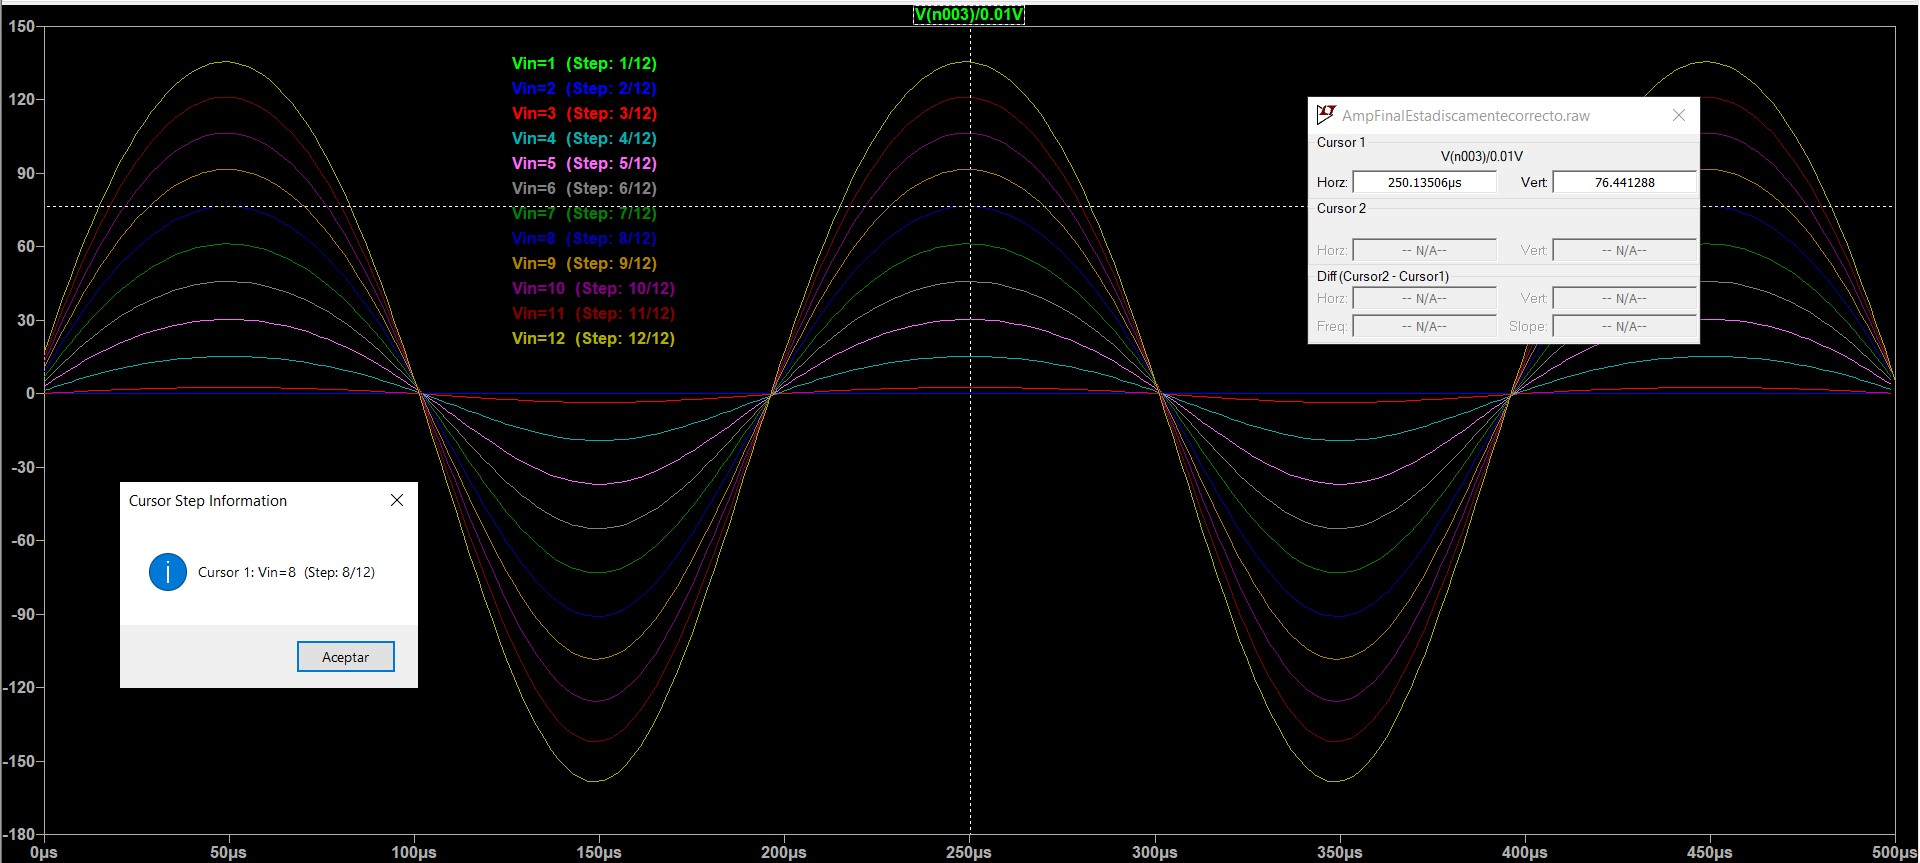
\includegraphics[width=\linewidth]{Simu/VCC-EMISOR.jpg}
        \caption{Variación de la fuente $V_{CC}$.}
      \label{SimuVarVccEC}
    \end{minipage}
\end{figure}

\begin{figure}[H]
    \centering
    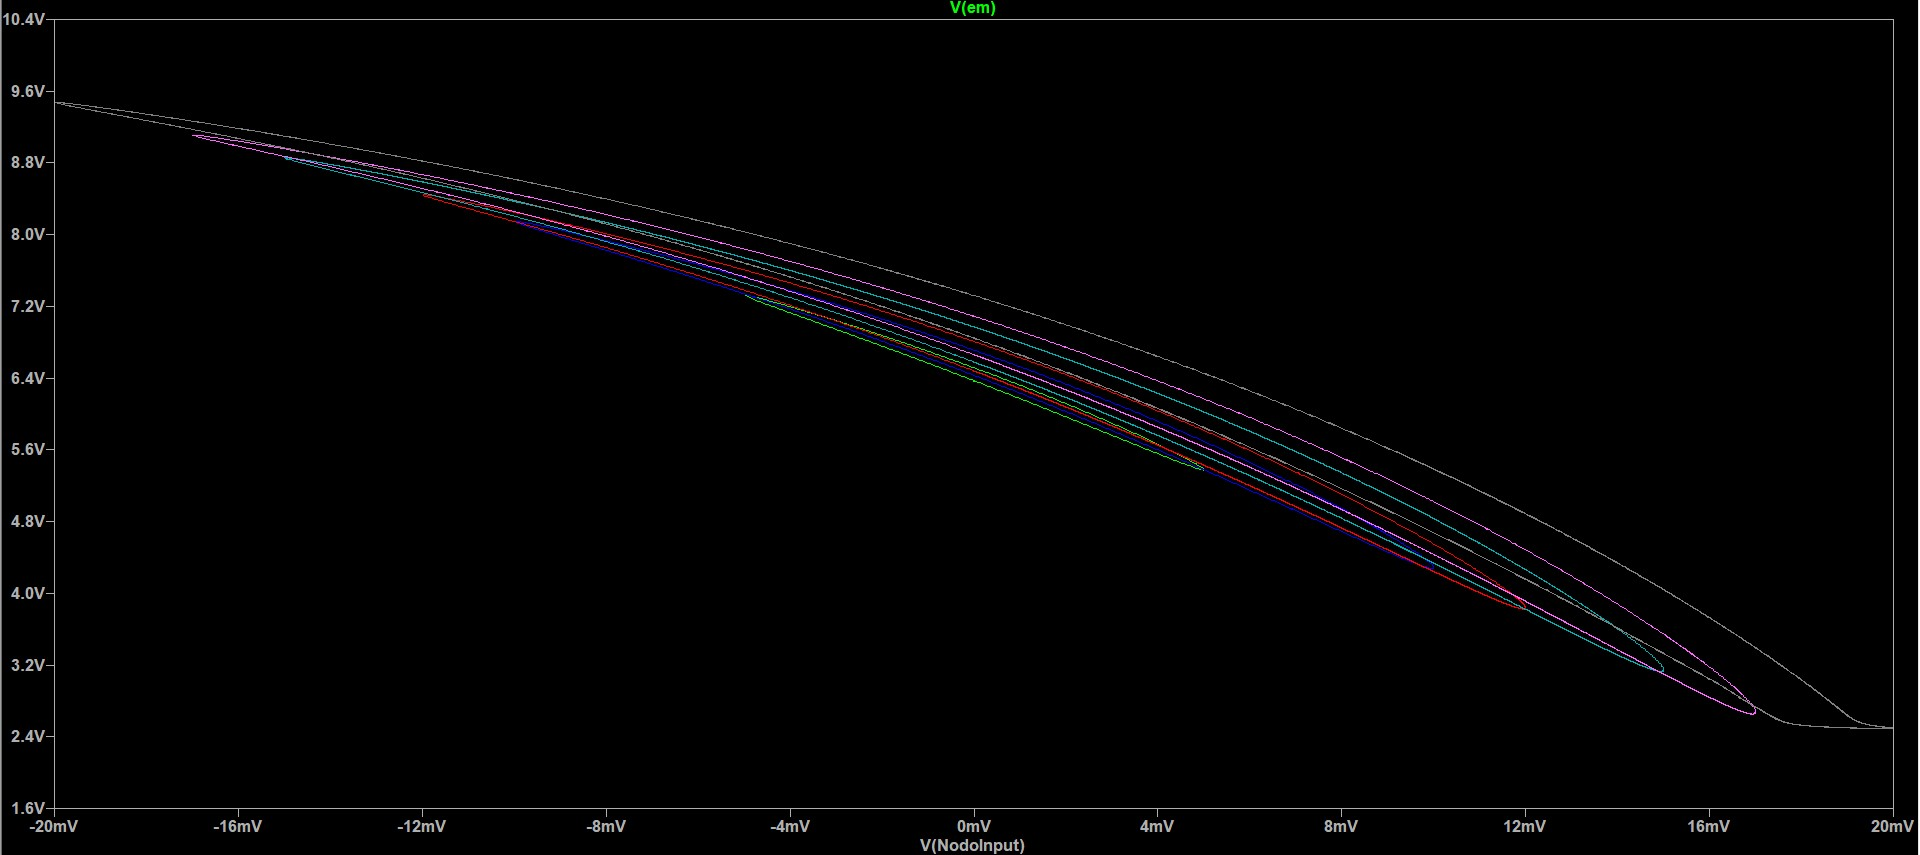
\includegraphics[width=0.75\linewidth]{Simu/Linealidad-em.jpg}
    \caption{Límites de linealidad de la etapa en Emisor Común.}
  \label{SimuLinEC}
\end{figure}
% =========================================================================
% APARTADO 4: ETAPA SZIKLAI
% =========================================================================
\subsubsection{Tercera Etapa: Salida Sziklai ($Q_4$ - $Q_5$)}
%\section{4. Tercera Etapa: Salida Sziklai ($Q_4$ - $Q_5$)}

\begin{figure}[H]
    \centering
    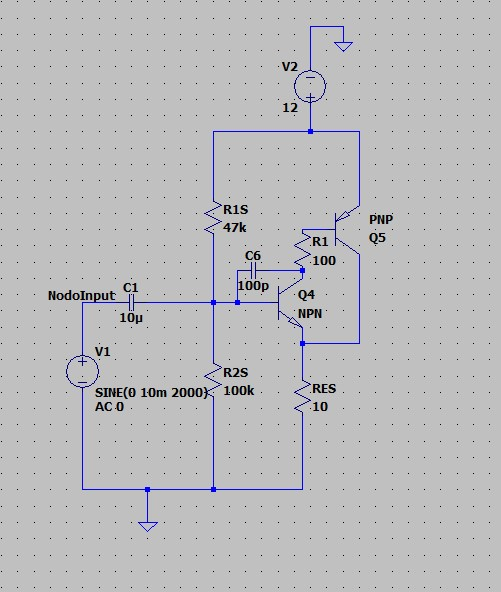
\includegraphics[width=0.45\linewidth]{Simu/sql-aislado.jpg}
    \caption{Circuito esquemático de la etapa de potencia Sziklai aislada.}
\end{figure}

\vspace{0.5em}
{\small\textbf{Polarización y Disipación de Potencia}}

%\subsubsection{4.1. Polarización y Disipación de Potencia}
Mediante \texttt{.op} se verificó la corriente de reposo que circula por los transistores $Q_4$ y $Q_5$ para confirmar la eliminación de la distorsión por cruce por cero (crossover).
\begin{verbatim}
.op
.meas DC I_Q4 I(Q4)
.meas DC I_Q5 I(Q5)
\end{verbatim}

\vspace{0.5em}
{\small\textbf{Medición de Impedancias de la Etapa Sziklai ($Z_{in3}$ y $Z_{out3}$)}}

%\subsubsection{4.2. Medición de Impedancias de la Etapa Sziklai ($Z_{in3}$ y $Z_{out3}$)}
Se determinó la impedancia de entrada vista desde la base de $Q_4$ y la impedancia de salida que presenta el par Sziklai hacia la carga de $8\,\Omega$.

\paragraph{Impedancia de Entrada ($Z_{in3}$)}
Se puede ver en (\cref{SimuZin3}).
\begin{figure}[H]
    \centering
    \begin{minipage}{0.48\textwidth}
        \centering
        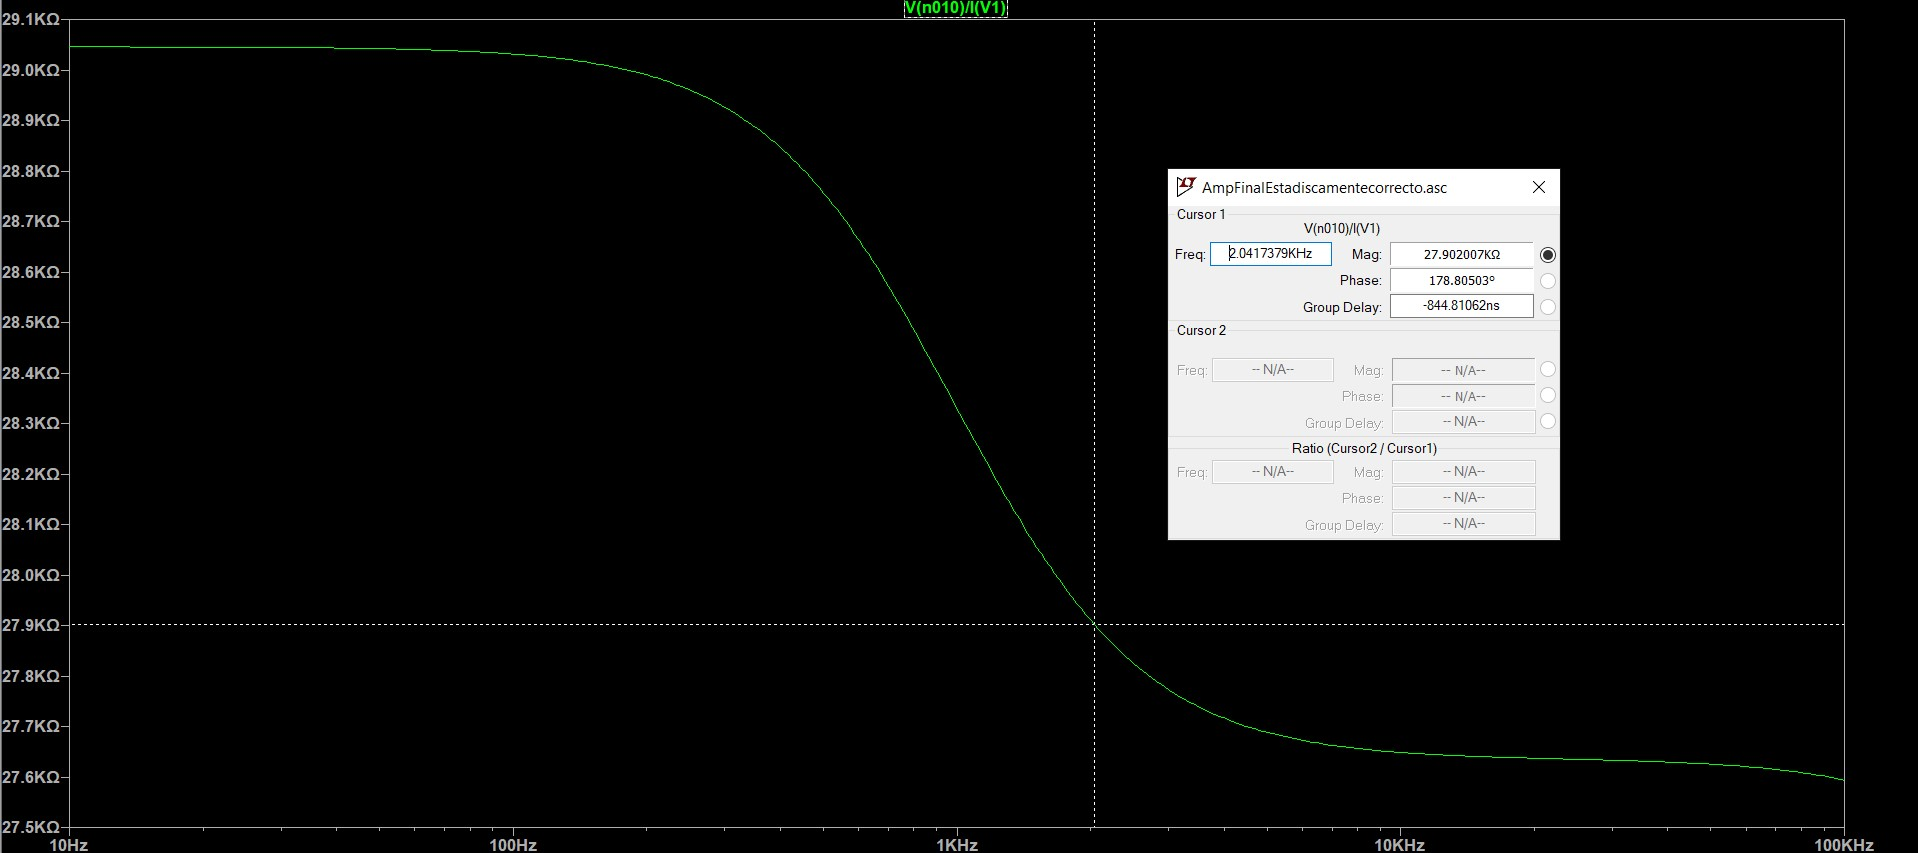
\includegraphics[width=\linewidth]{Simu/SQL_ZIN.jpg}
        \caption{Curva de respuesta de $Z_{in3}$.}
      \label{SimuZin3}
    \end{minipage}
\end{figure}

\paragraph{Impedancia de Salida ($Z_{out3}$)}
Se puede ver en (\cref{SimuZout3}).
\begin{figure}[H]
    \centering
    \begin{minipage}{0.48\textwidth}
        \centering
        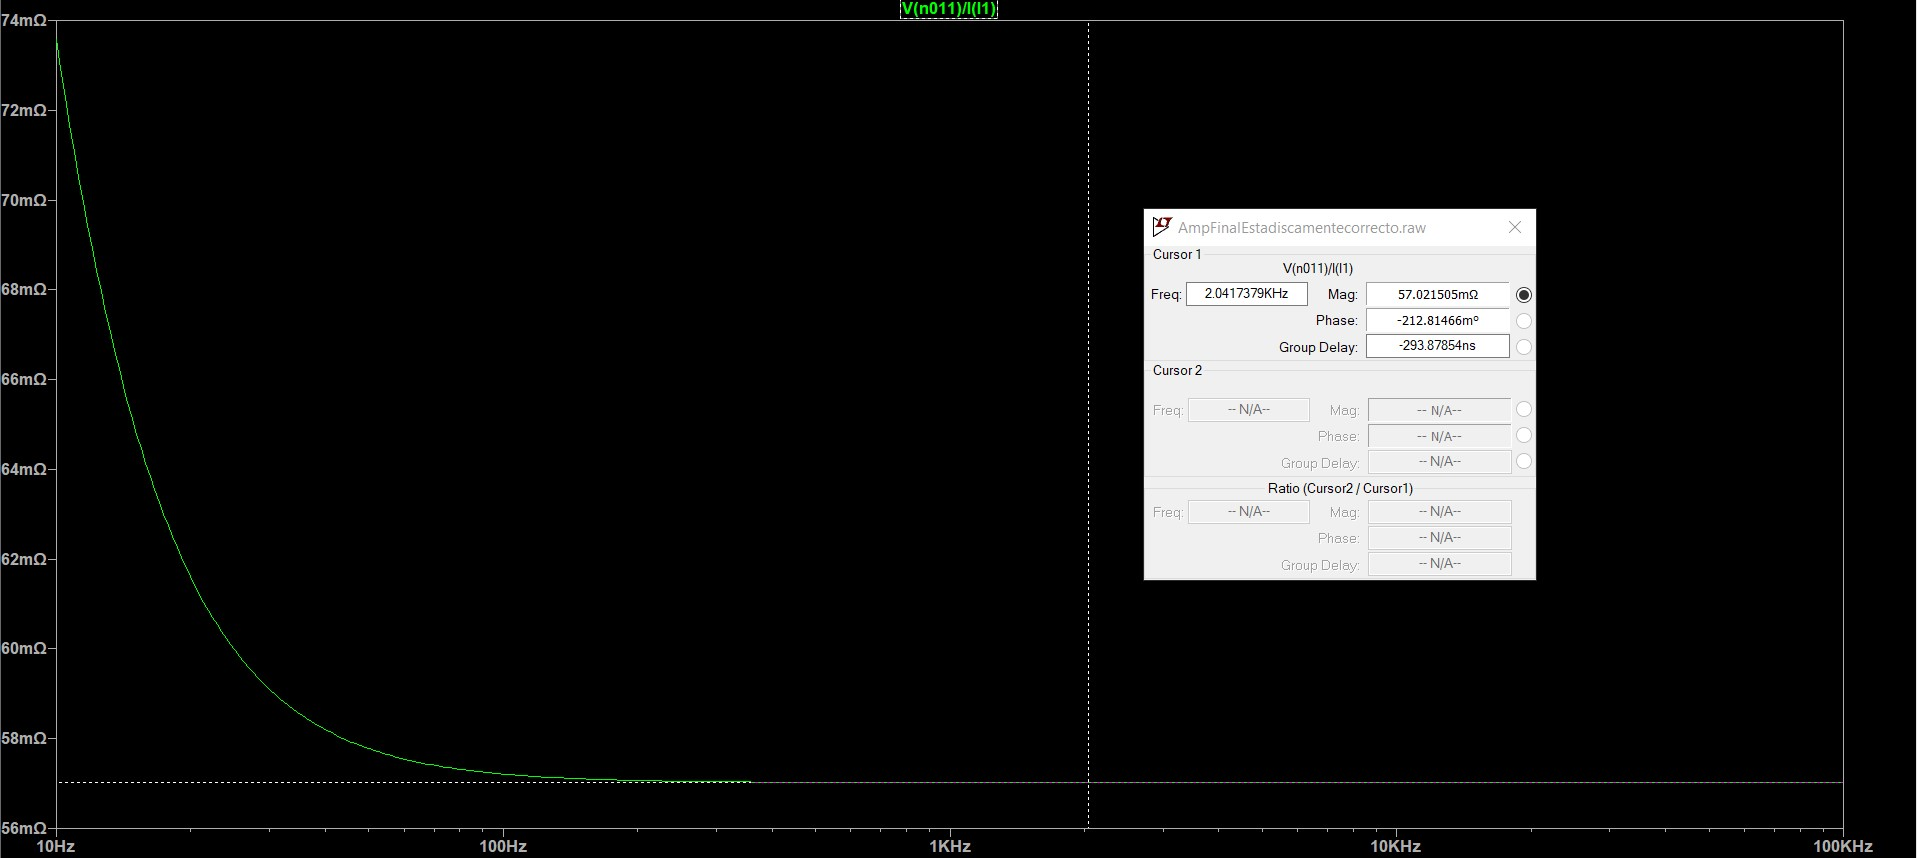
\includegraphics[width=\linewidth]{Simu/SQL_ZOUT.jpg}
        \caption{Curva de respuesta de $Z_{out3}$.}
      \label{SimuZout3}
    \end{minipage}
\end{figure}

\vspace{0.5em}
{\small\textbf{Respuesta en Frecuencia, Temporal, Ruido, Límites de $V_{CC}$ y Linealidad)}}

%\subsubsection{4.3. Respuesta en Frecuencia, Temporal, Ruido, Límites de $V_{CC}$ y Linealidad}
  Se evaluó el comportamiento de la etapa Sziklai en régimen dinámico, registrando el ancho de banda (\texttt{.ac}), la respuesta temporal (\texttt{.tran}), el ruido (\texttt{.noise}), la tolerancia ante variaciones de la fuente $V_{CC}$ y el límite de linealidad antes del recorte (\cref{SimuBWSz}, \cref{SimuTepSz}, \cref{SimuPSDSz}, \cref{SimuVarVccSz}, \cref{SimuLinSz}).

\begin{figure}[H]
    \centering
    \begin{minipage}{0.48\textwidth}
        \centering
        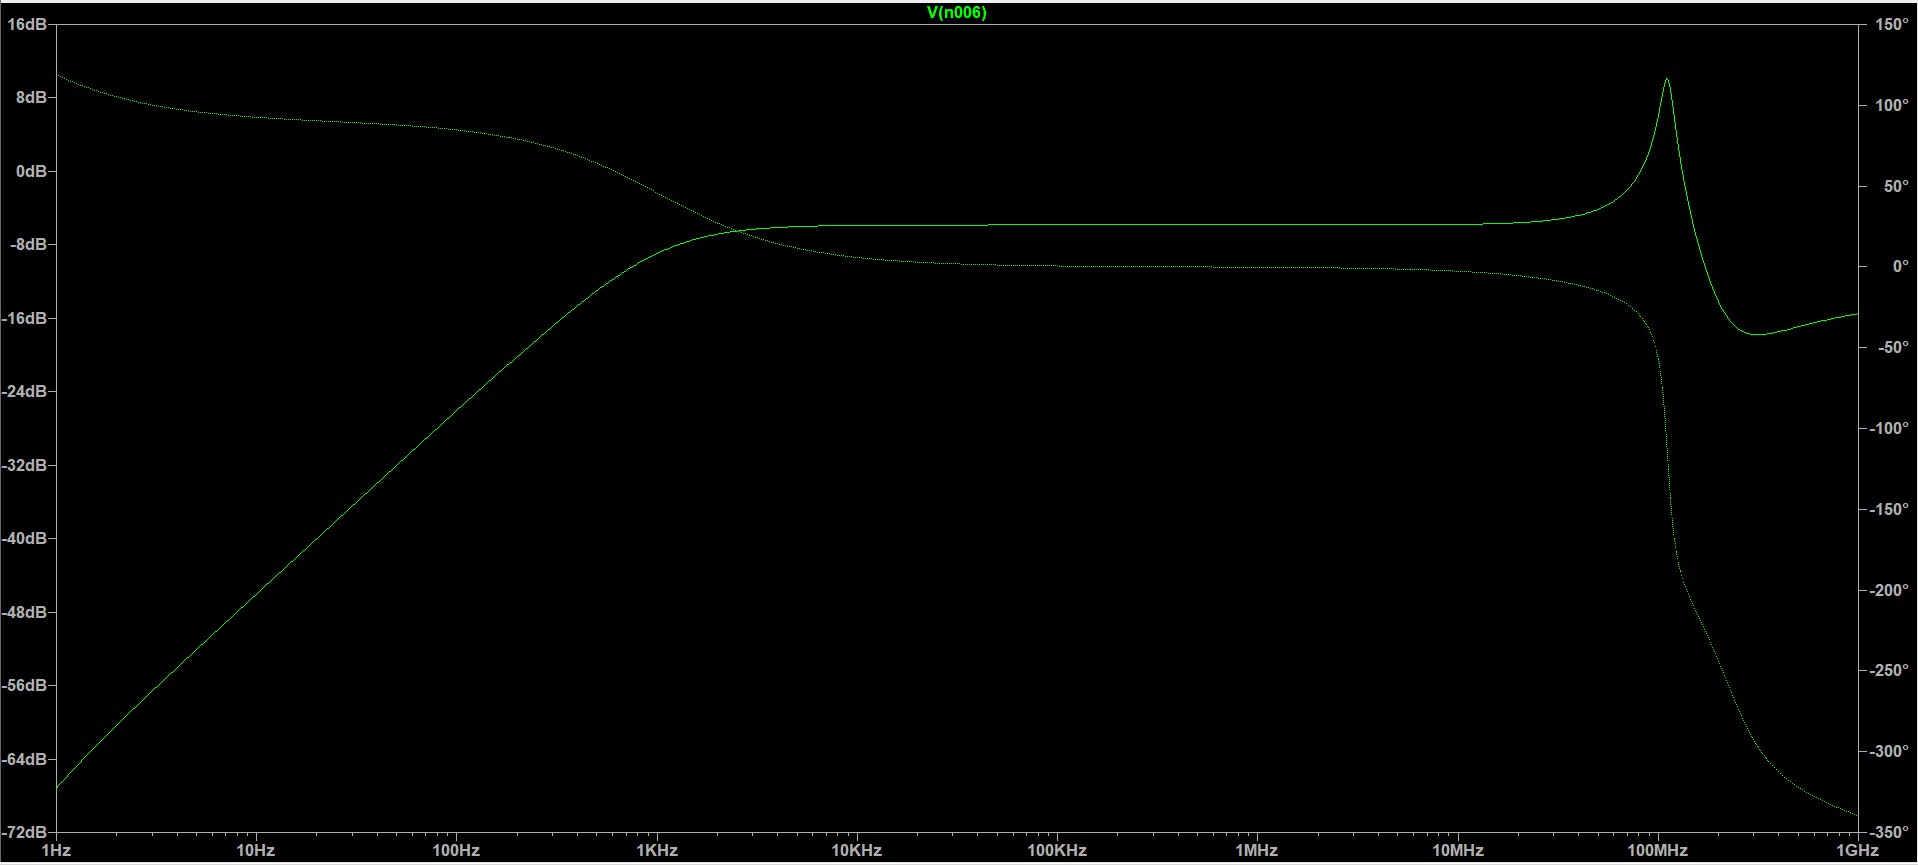
\includegraphics[width=\linewidth]{Simu/BW-SQL.jpg}
        \caption{Ancho de banda - Etapa Sziklai.}
      \label{SimuBWSz}
    \end{minipage}\hfill
    \begin{minipage}{0.48\textwidth}
        \centering
        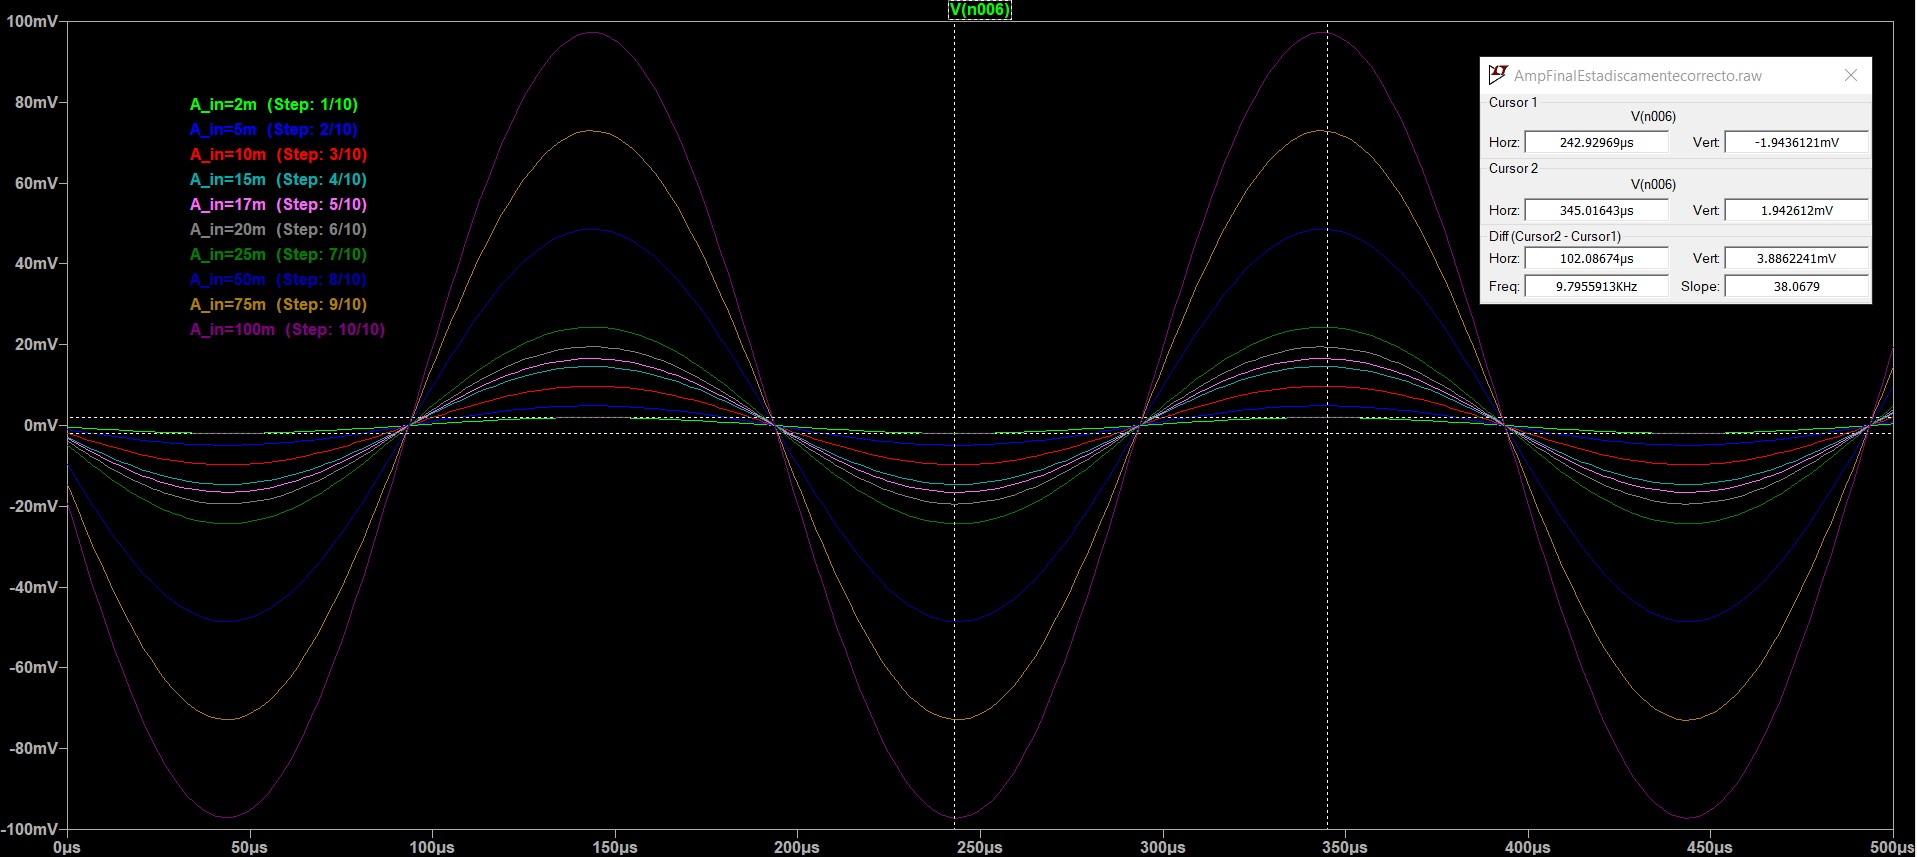
\includegraphics[width=\linewidth]{Simu/VPP-SQL.jpg}
        \caption{Respuesta temporal en la carga.}
      \label{SimuTepSz}
    \end{minipage}
\end{figure}

\begin{figure}[H]
    \centering
    \begin{minipage}{0.48\textwidth}
        \centering
        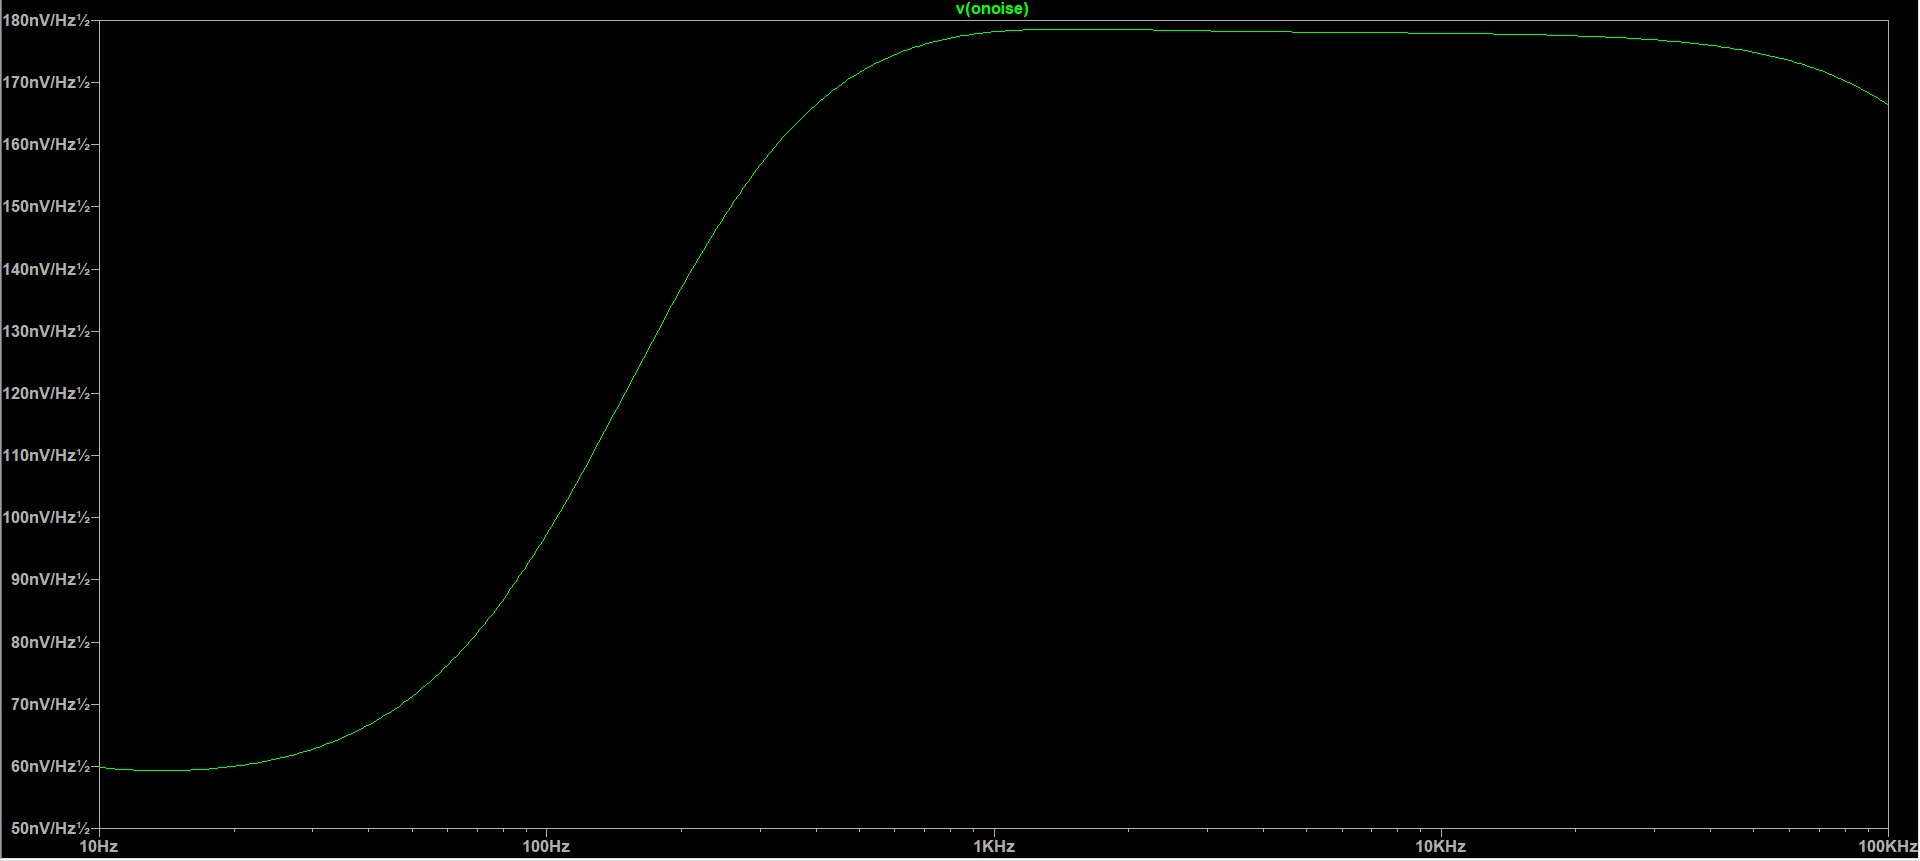
\includegraphics[width=\linewidth]{Simu/NOISE-SQL.jpg}
        \caption{PSD de Ruido - Etapa Sziklai.}
      \label{SimuPSDSz}
    \end{minipage}\hfill
    \begin{minipage}{0.48\textwidth}
        \centering
        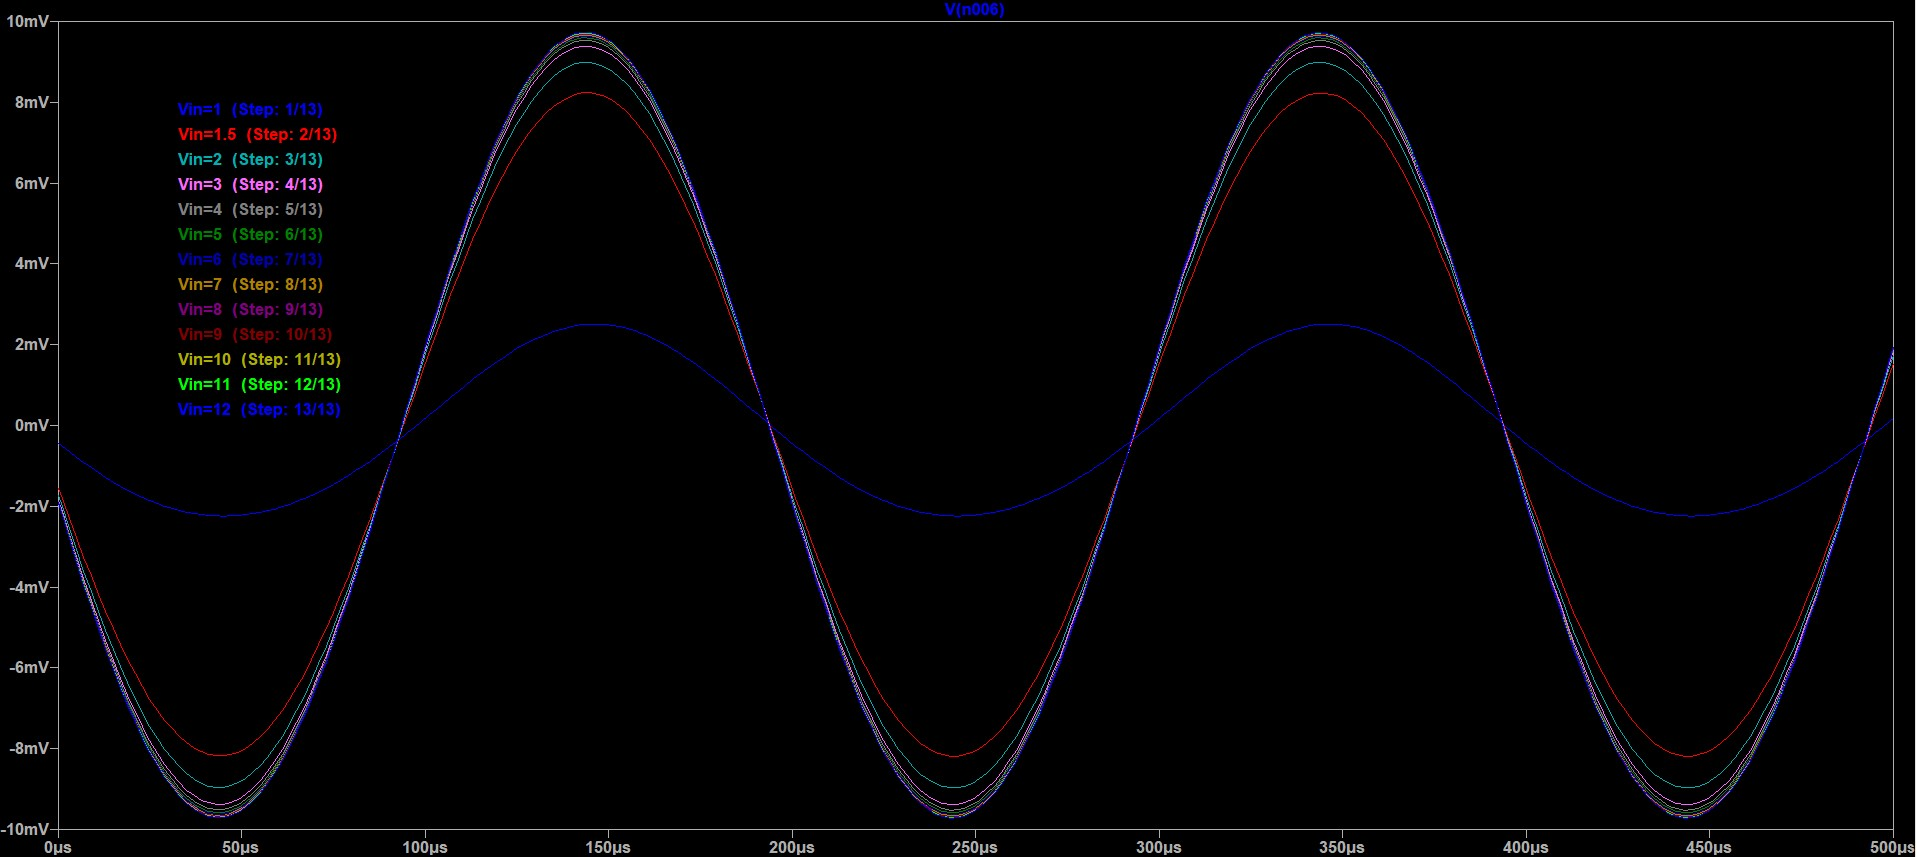
\includegraphics[width=\linewidth]{Simu/vcc-sql.jpg}
        \caption{Variación de la fuente $V_{CC}$.}
      \label{SimuVarVccSz}
    \end{minipage}
\end{figure}

\begin{figure}[H]
    \centering
    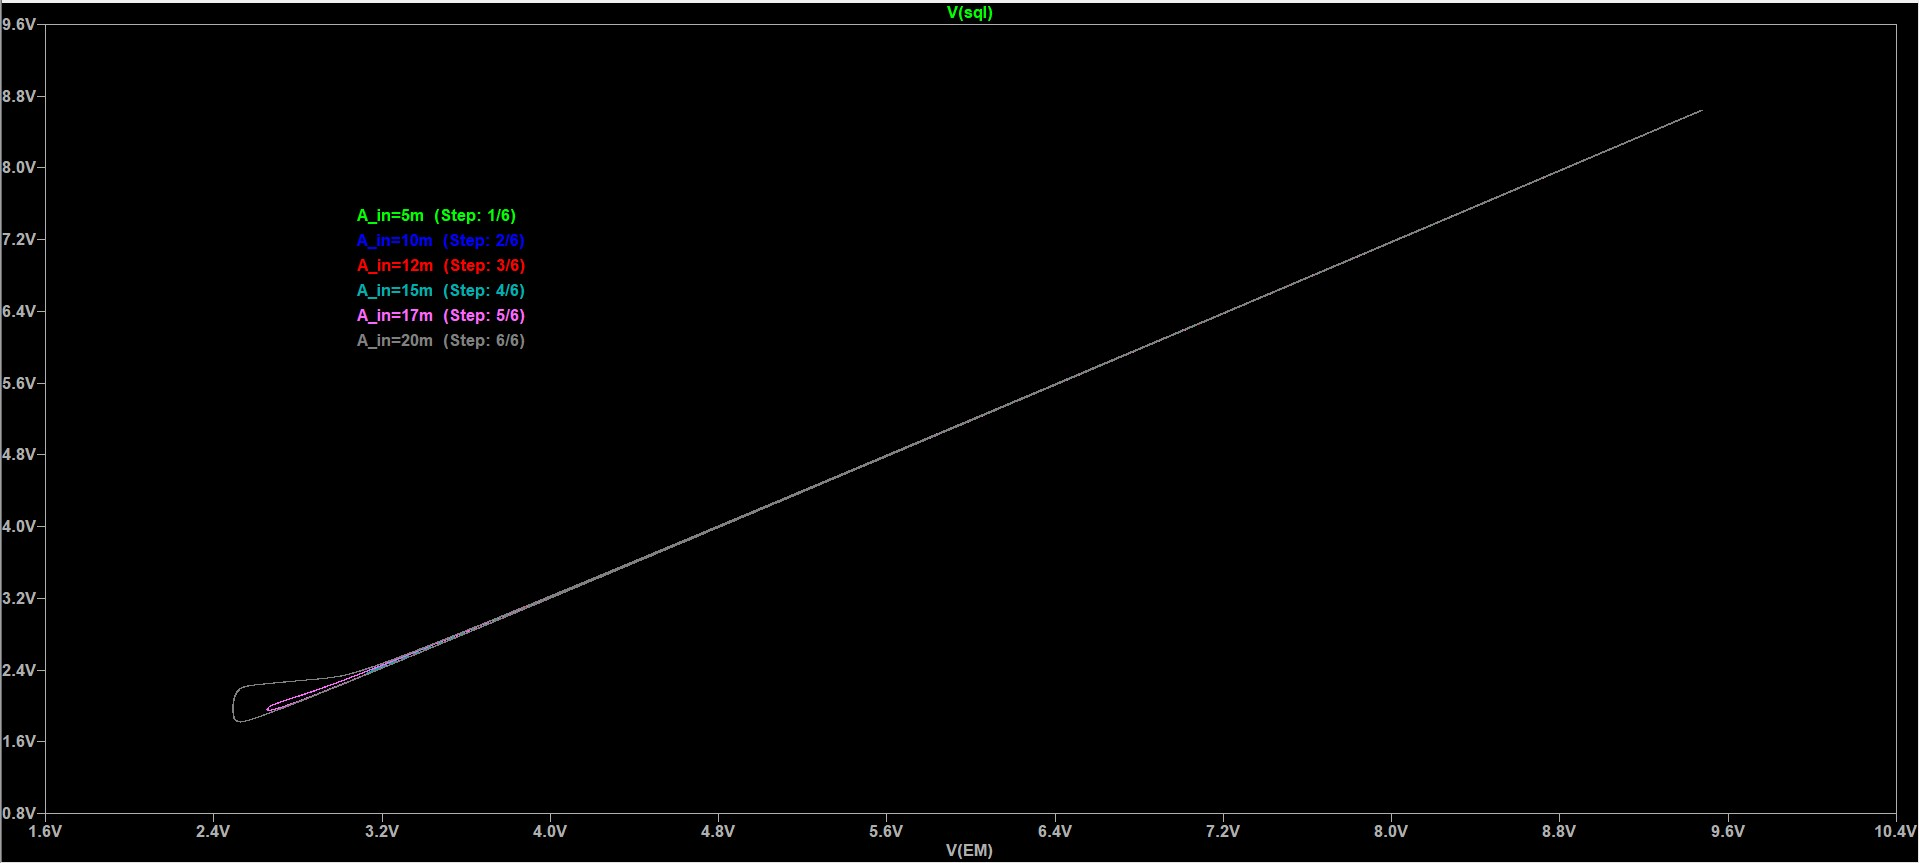
\includegraphics[width=0.75\linewidth]{Simu/Linealidad-sql.jpg}
    \caption{Límites de linealidad de la etapa Sziklai observando la salida.}
  \label{SimuLinSz}
\end{figure}

% =========================================================================
% APARTADO 5: NOTA ACLARATORIA SOBRE EL ALCANCE DE LAS SIMULACIONES
% =========================================================================

\subsubsection{Consideraciones sobre la Presentación y Documentación de los Resultados}
%\section{5. Consideraciones sobre la Presentación y Documentación de los Resultados}

Cabe destacar que la metodología analítica y los procedimientos de medición simulada expuestos de forma detallada en el análisis global (Sección 1) fueron aplicados de manera idéntica y sistemática pa cada una de las etapas del amplificador (Darlington, Emisor Común y Sziklai).

Con el objetivo de mantener la concisión, fluidez y claridad en la lecturao, la exposición gráfica en las Secciones 2, 3 y 4 se ha presentado de forma sintetizada, incorporando únicamente las figuras y curvas de respuesta consideradas más representativas para la comprensión del comportamiento de cada etapa aislada.

No obstante, la totalidad de los ensayos de simulación se encuentran  documentados y disponibles para su consulta y verificación en el repositorio de GitHub asociado a este trabajo práctico.


\subsection{Medición}

A continuacion se establecerá como fueron ejecutadas las mediciones del circuito construido. Los esquemas se elaboraron en proteus y son representativos, se debe hacer caso omiso a la nomenclatura de estos. Es importante mencionar que el generador de señales es representado en los esquematicos como una fuente de tension AC.

\subsection{Setup General}
A continuación se vera un acercamiento a las formas de las mediciones a nivel general, las conexiones utilizadas y el espacio de trabajo.

\begin{figure}[H]
    \centering
    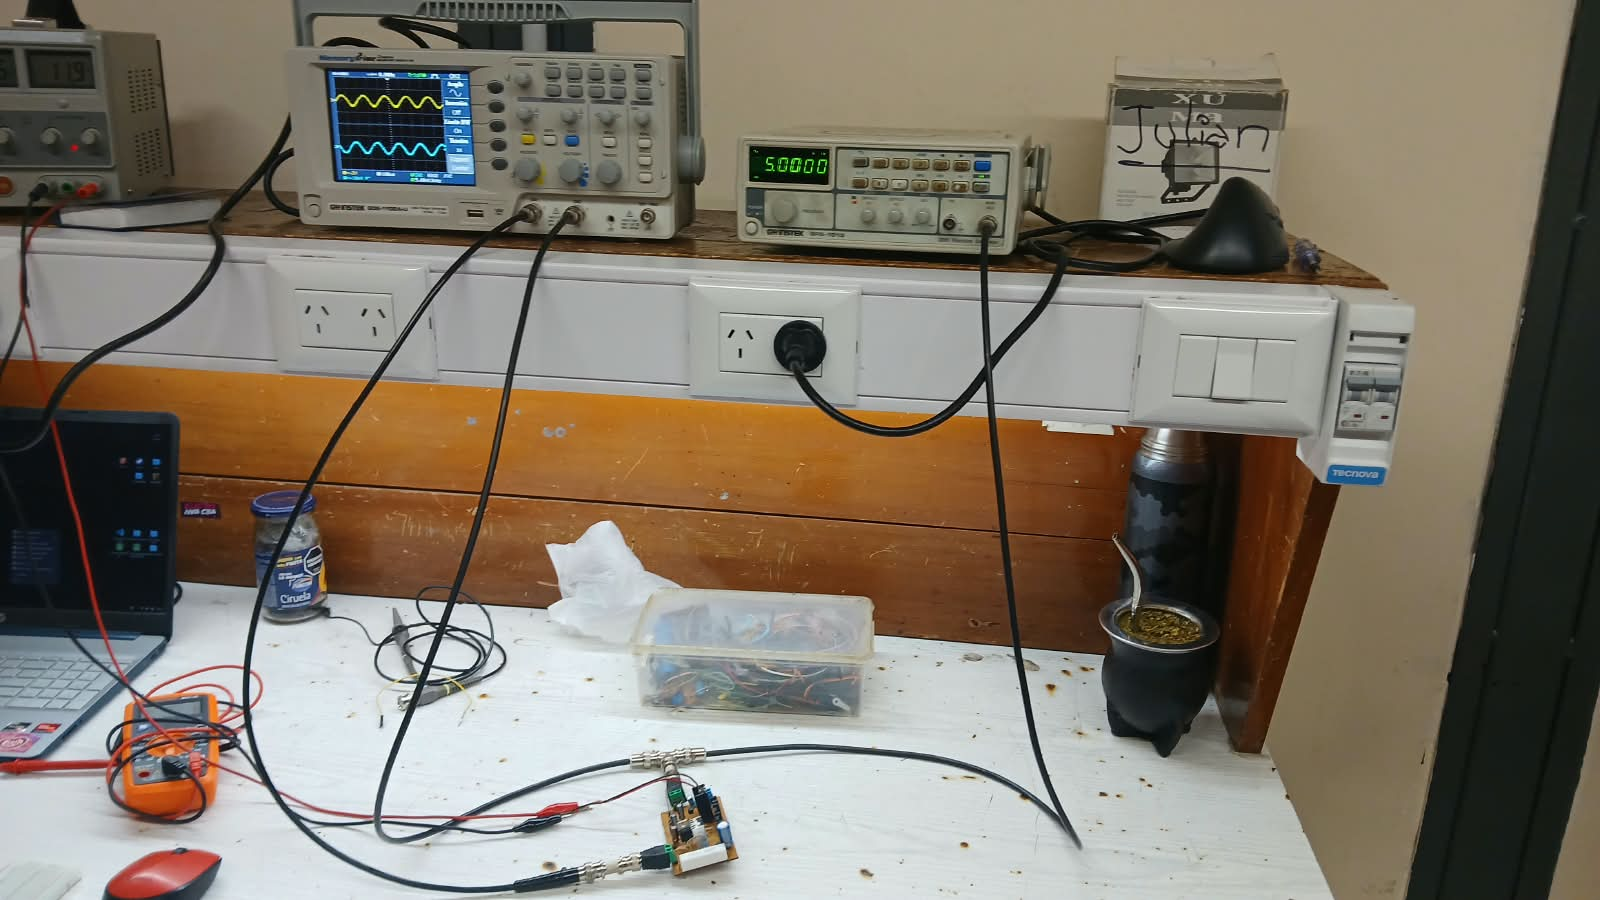
\includegraphics[width=0.8\textwidth]{FotosMed/Setup/SetupGeneral1.jpeg}
    \caption{Distribucion General}
    \label{fig:DistribucionGeneral}
\end{figure}

\begin{figure}[H]
    \centering
    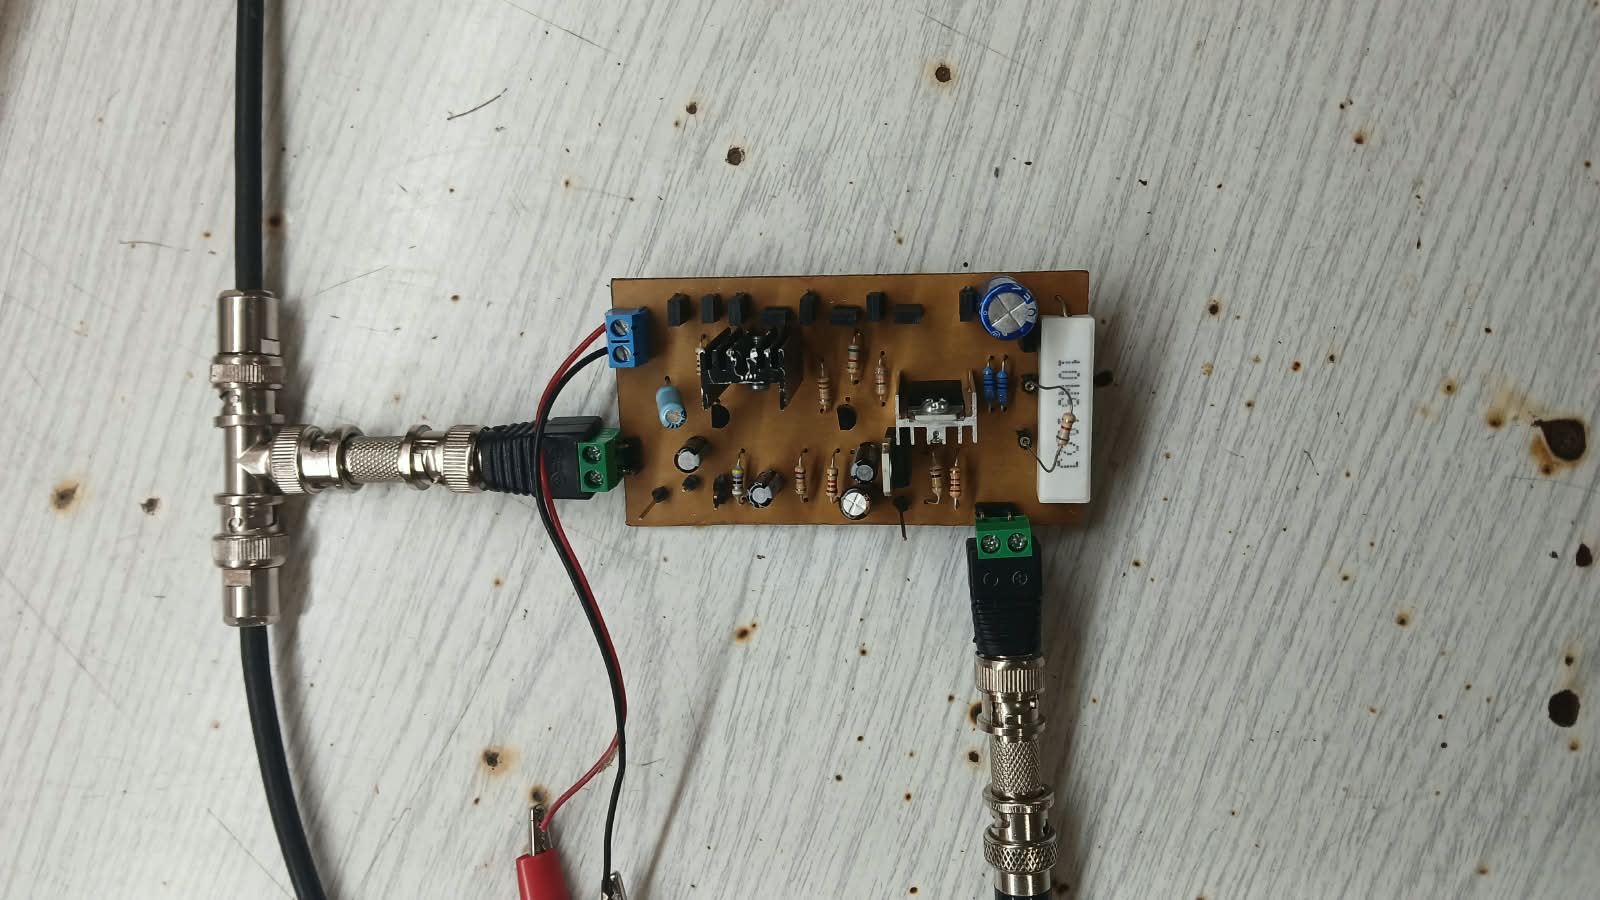
\includegraphics[width=0.8\textwidth]{FotosMed/Setup/PlacaConectada.jpeg}
    \caption{Conexion a Placa}
    \label{fig:placa}
\end{figure}

\begin{figure}[H]
    \centering
    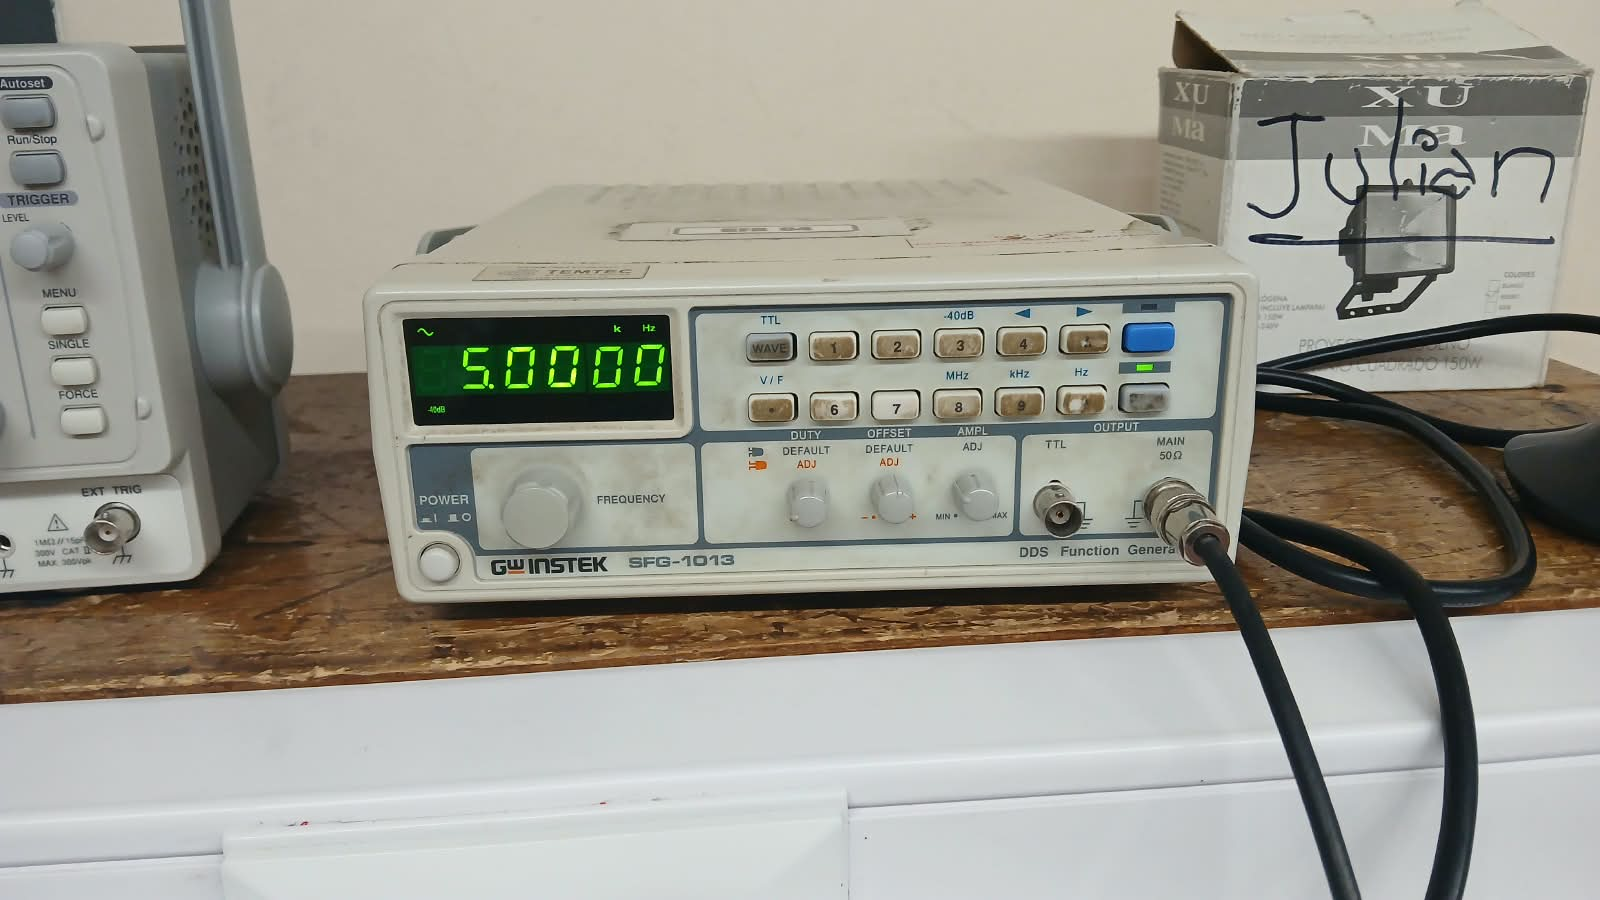
\includegraphics[width=0.8\textwidth]{FotosMed/Setup/Generador.jpeg}
    \caption{Generador}
    \label{fig:GeneradorGeneral}
\end{figure}

\begin{figure}[H]
    \centering
    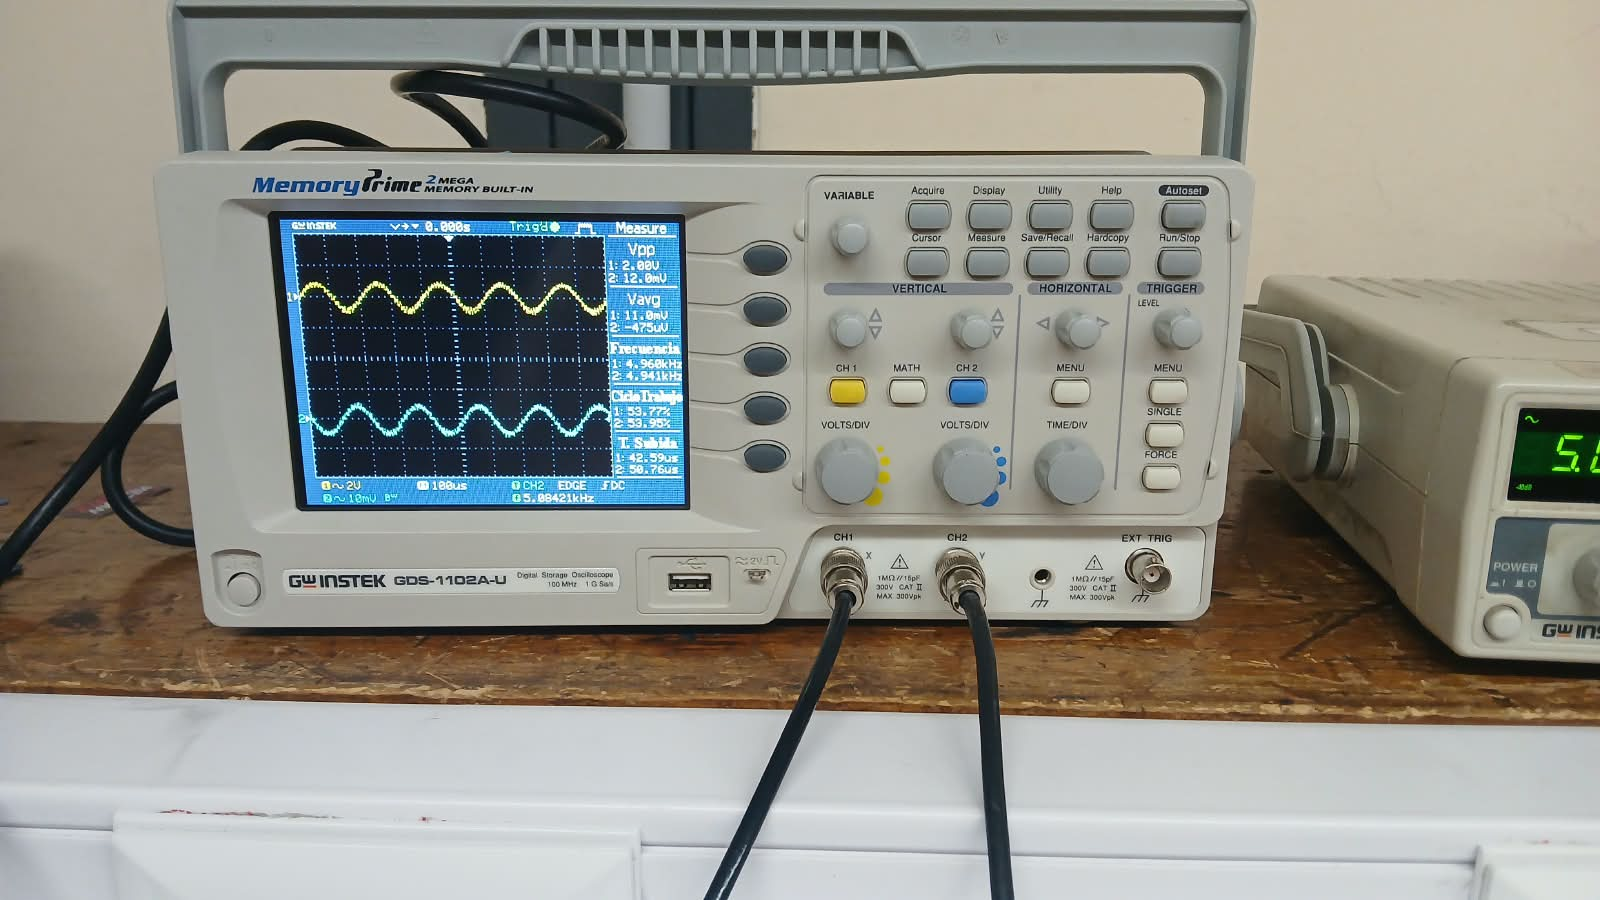
\includegraphics[width=0.8\textwidth]{FotosMed/Setup/Osc.jpeg}
    \caption{Osciloscopio}
    \label{fig:OscGeneral}
\end{figure}


\subsection{Medicion de Transistores}
Realizadas con el multímetro de trabajo, se evaluaron la caída de tensión de cada uno de los componentes teniendo precauciones de evitar el contacto entre terminales. Se aprovecharon los jumpers incluidos en el disenio para realizar las mediciones de corriente de colector de los transistores.

\begin{figure}[H]
    \centering
    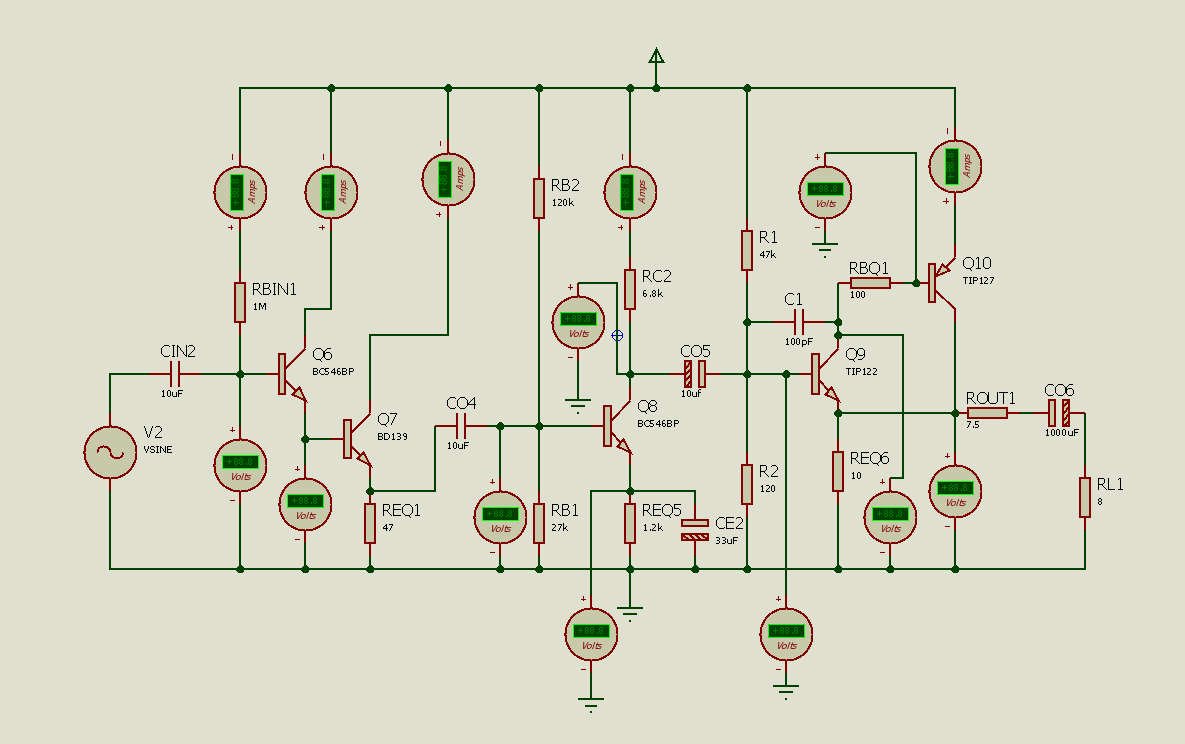
\includegraphics[width=0.8\textwidth]{SetupMediciones/TensionesCorrientes/VITransistores.png}
    \caption{Esquema de Medición de Transistores}
    \label{fig:esquematicoTransistores}
\end{figure}

Como se puede observar en la Figura \ref{fig:esquematicoTransistores}, estas mediciones de tension y corriente fueron exclusivamente realizadas para el calculo de potencia de los transistores, se debe remarcar aqui que la corriente de colector del transistor NPN del Sziklai fue hecha de manera indirecta, midiendo la caida de tension en la resistencia de base del pnp.

\begin{figure}[H]
    \centering
    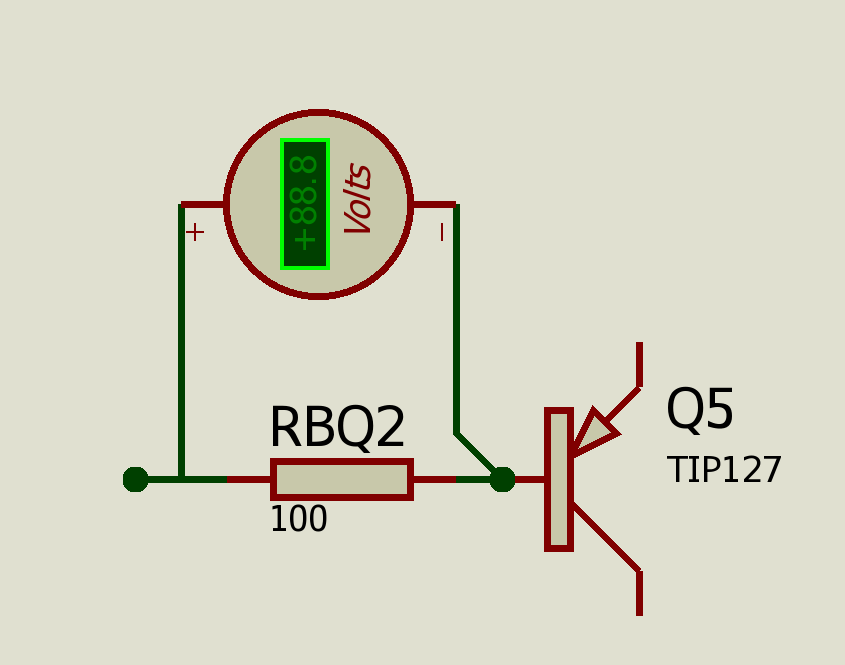
\includegraphics[width=0.8\textwidth]{SetupMediciones/TensionesCorrientes/IcQ4.png}
    \caption{Medición Indirecta}
    \label{fig:esquematicoICQ4}
\end{figure}

Como se puede observar en la Figura \ref{fig:esquematicoICQ4}, una vez medida la tension de la resistencia, se obtuvo Ic para los cálculos de potencia.

\subsection{Medición de Resistencias}
Similar al caso anterior, estas también fueron ejecutadas mediante un multímetro digital.

\begin{figure}[H]
    \centering
    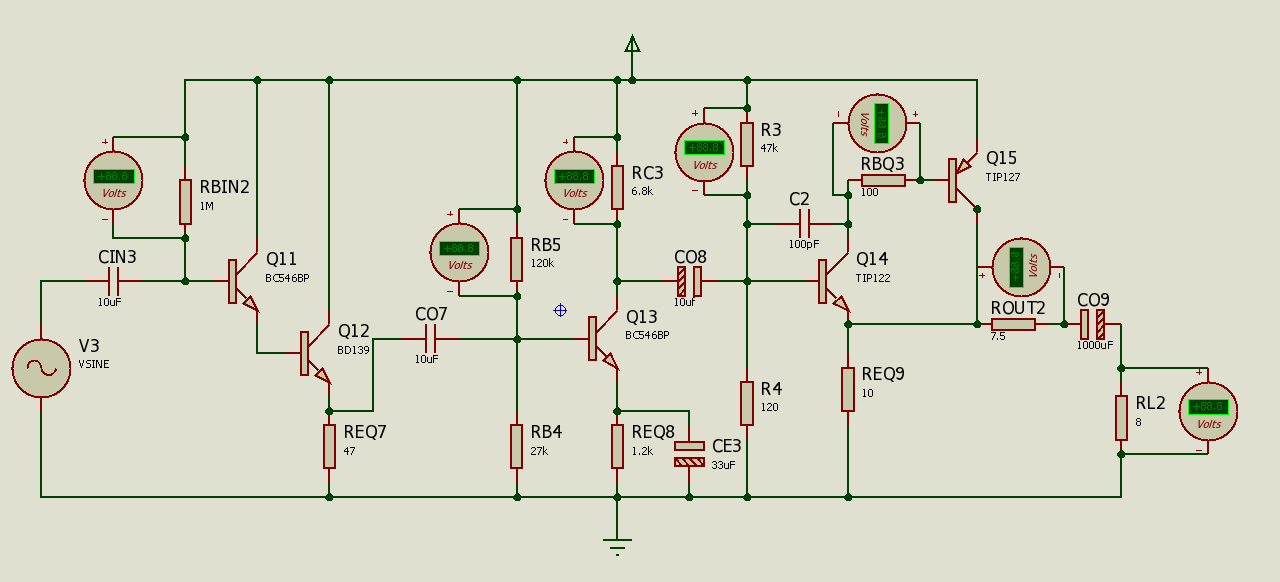
\includegraphics[width=0.8\textwidth]{SetupMediciones/TensionesCorrientes/VResitecnias.png}
    \caption{Esquema de Medición de Resistencias}
    \label{fig:esquematicoResistencias}
\end{figure}

Una vez obtenidas las mediciones de la Figura \ref{fig:esquematicoResistencias}, se determino la potencia disipada mediante la Ley de Ohm.

\subsection{Barrido de Amplitud}
Esta medición es realizada en 3 configuraciones:
    - Darlington
    - Darlinton y Emisor Comun
    - Circuito completo

En esta, las amplitudes de entrada a las configuraciones irán aumentando, esto se realizo incrementando la amplitud de salida del generador de señales.

\subsubsection{Barrido de Etapa 1}
A conitunuacion se presenta el esquema y foto del método de medicion utilizado en la etapa 1(Darlington).

\begin{figure}[H]
    \centering
    % Primera minipage (ocupa el 45% del ancho de la página)
    \begin{minipage}{0.45\textwidth}
        \centering
        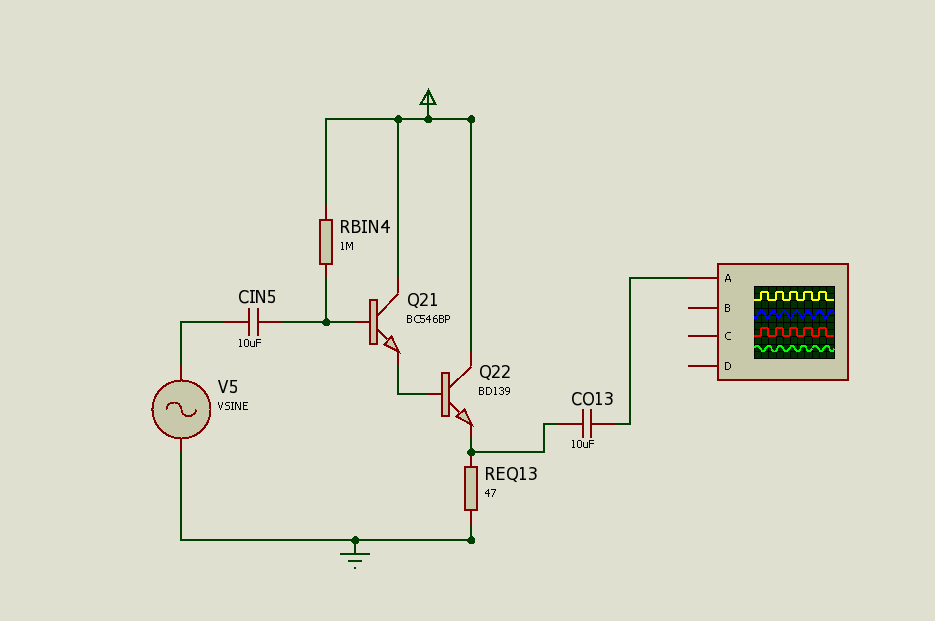
\includegraphics[width=\textwidth]{SetupMediciones/TensionesCorrientes/VMaxMinDAR.png} % Ajusta el ancho al de la minipage
        \caption{Representacion esquematica.}
        \label{fig:esquematicpBarridoEtapa1}
    \end{minipage}
    \hfill % Relleno elástico para separar las imágenes
    % Segunda minipage (ocupa el 45% del ancho de la página)
    \begin{minipage}{0.45\textwidth}
        \centering        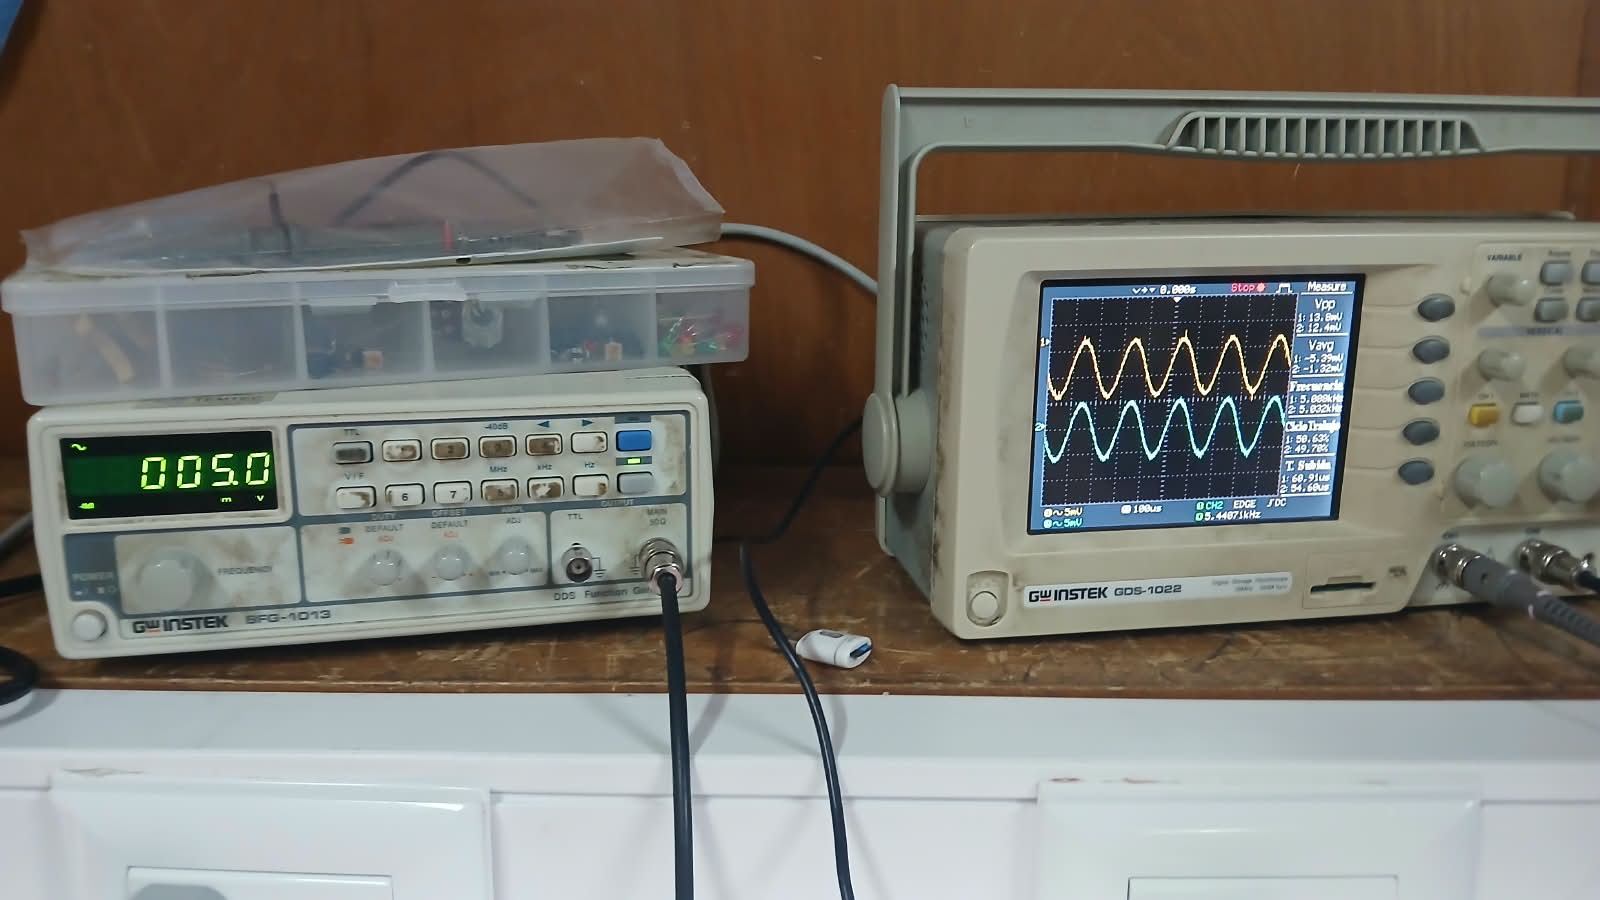
\includegraphics[width=\textwidth]{FotosMed/Barrido de amplitud/E1/5m.jpeg}
        \caption{Imagen de la Medicion.}
        \label{fig:medicionBarridoEtapa1}
    \end{minipage}
\end{figure}

\begin{figure}[H]
    \centering
    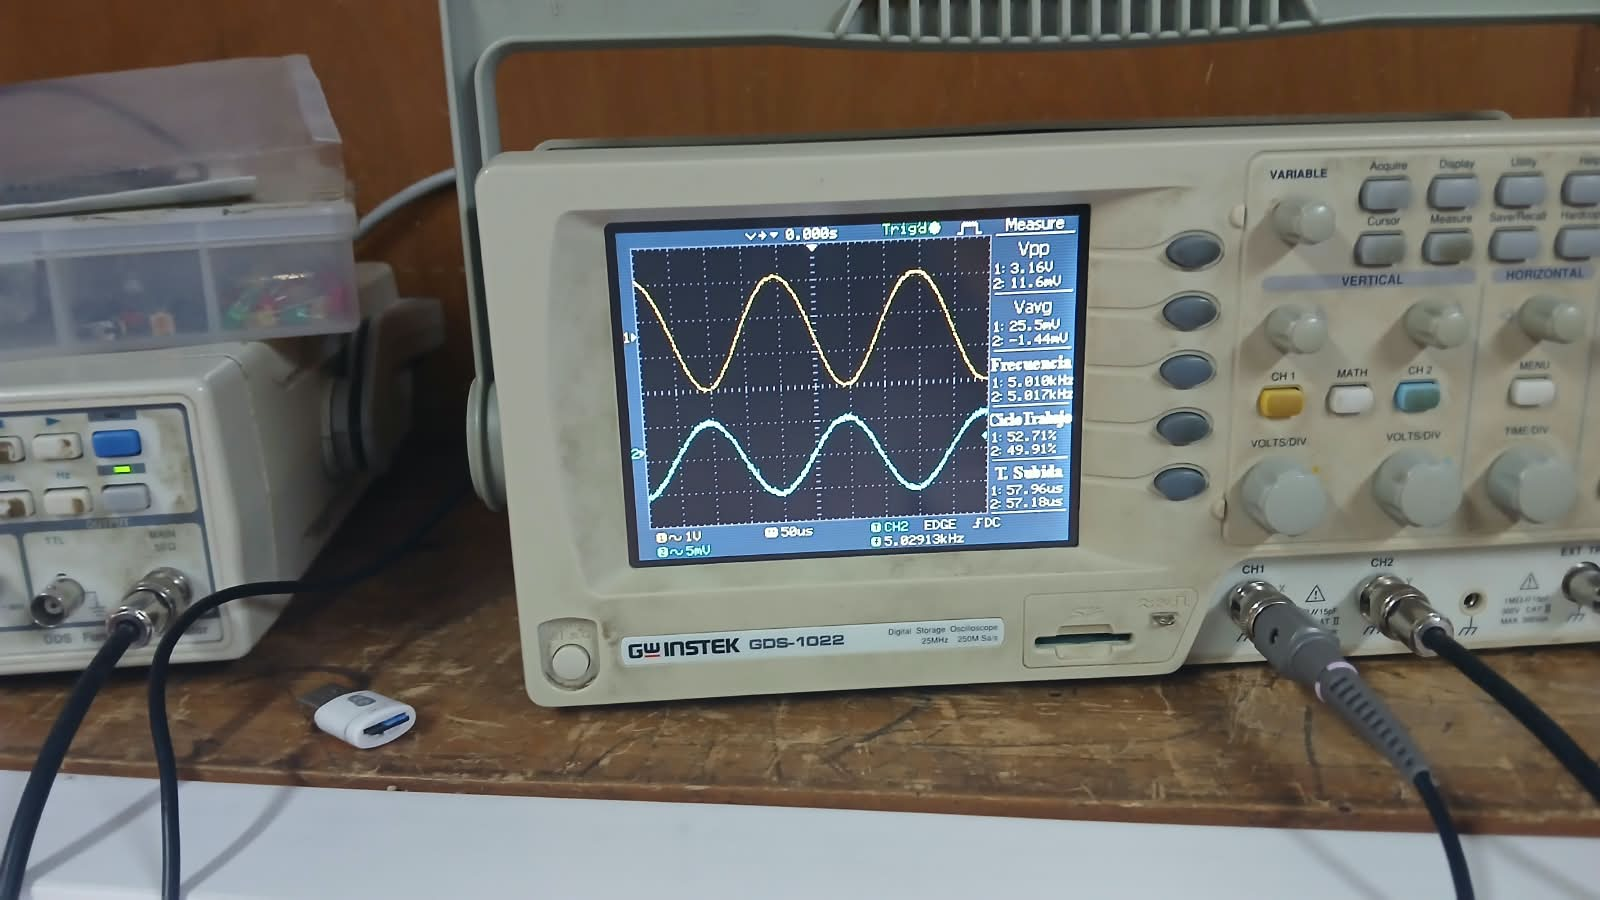
\includegraphics[width=0.8\textwidth]{FotosMed/Barrido de amplitud/E12/5mzoom.jpeg}
    \caption{Pantalla del Osciloscopio}
    \label{fig:osciloscopioBarridoEtapa1}
\end{figure}

Se puede ver en \ref{fig:osciloscopioBarridoEtapa1}, la tension de entrada esta en el canal 1 del osciloscopio (estipulada a 13.8 mV pico a pico) mientras que la salida se observa en el canal 2.

\subsubsection{Barrido de Etapa 1 y 2}
Semejante al anterior, la tensión de entrada sigue siendo variada incrementando el dial del generador en modo amplitud, con la leve diferencia de que esta configuración esta constituida por las etapas 1 y 2 en conjunto.

\begin{figure}[H]
    \centering
    % Primera minipage (ocupa el 45% del ancho de la página)
    \begin{minipage}{0.45\textwidth}
        \centering
        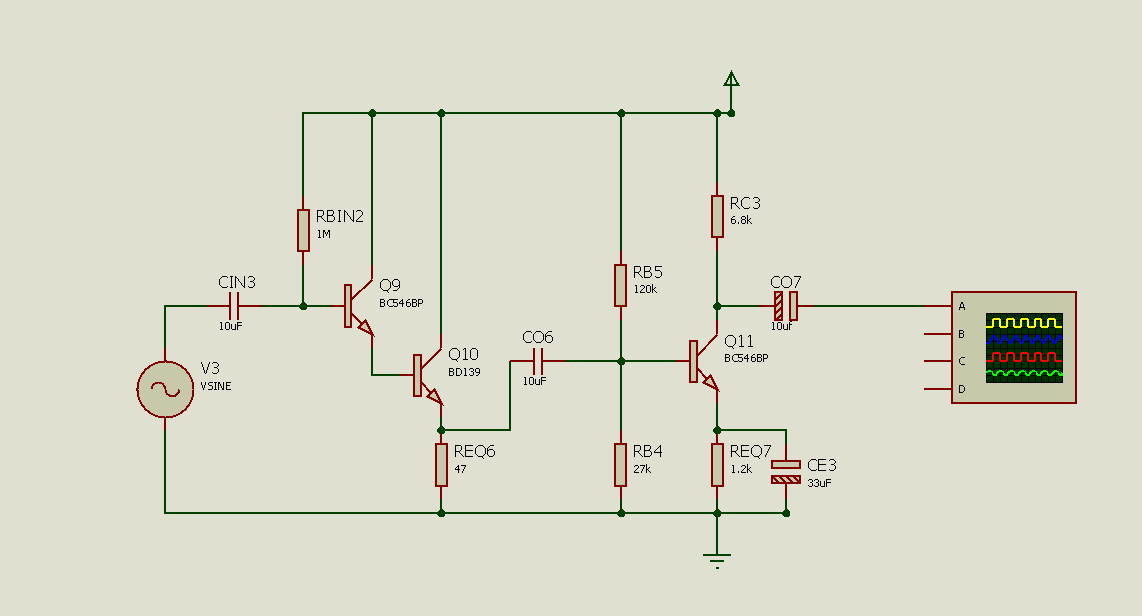
\includegraphics[width=\textwidth]{SetupMediciones/ZOUT/Zout12VACIO.png} % Ajusta el ancho al de la minipage
        \caption{Representacion esquematica.}
        \label{fig:esquematicpBar12}
    \end{minipage}
    \hfill % Relleno elástico para separar las imágenes
    % Segunda minipage (ocupa el 45% del ancho de la página)
    \begin{minipage}{0.45\textwidth}
        \centering
        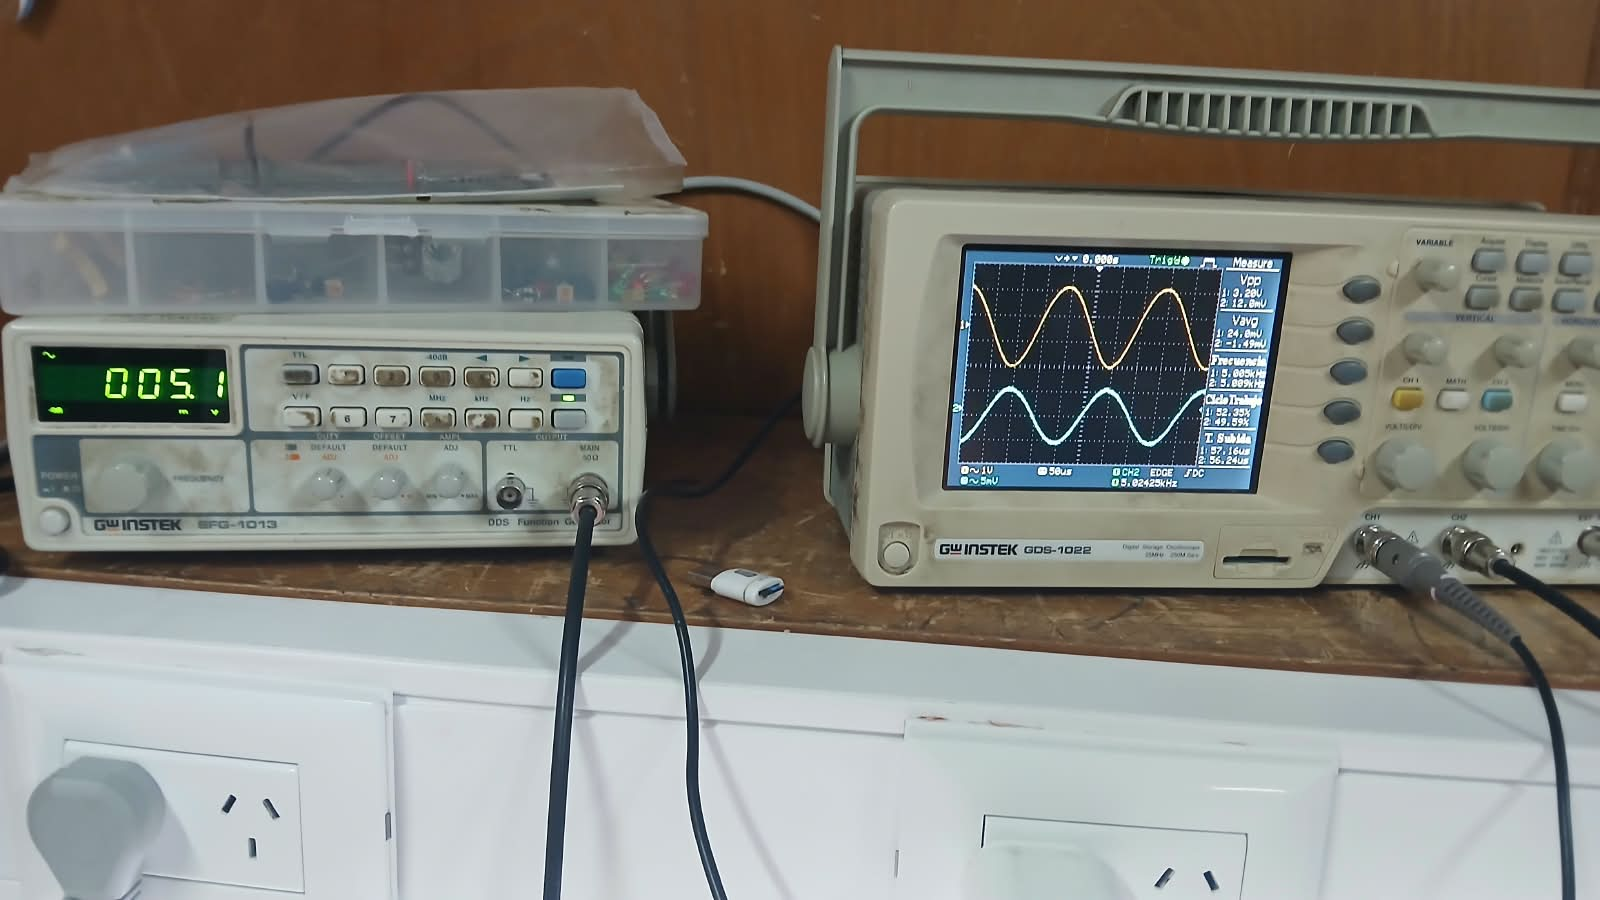
\includegraphics[width=\textwidth]{FotosMed/Barrido de amplitud/E12/5m.jpeg}
        \caption{Imagen de la Medicion.}
        \label{fig:medicionbar12}
    \end{minipage}
\end{figure}

\begin{figure}[H]
    \centering
    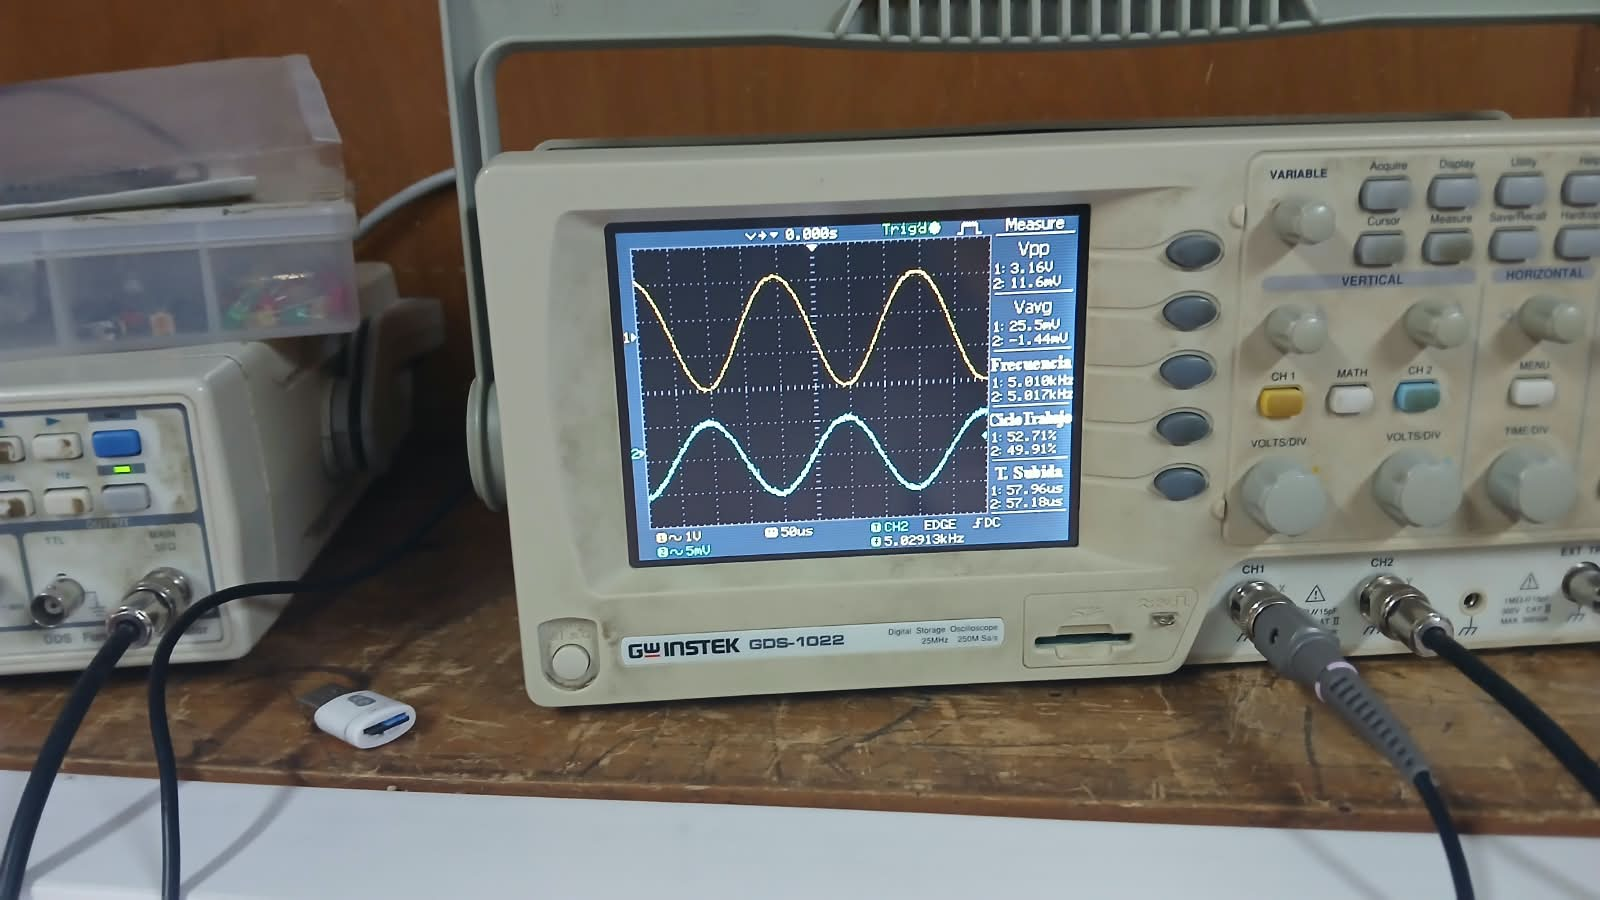
\includegraphics[width=0.8\textwidth]{FotosMed/Barrido de amplitud/E12/5mzoom.jpeg}
    \caption{Pantalla del Osciloscopio}
    \label{fig:osciloscopioBArr12}
\end{figure}

Se puede ver en \ref{fig:osciloscopioBArr12} la tension de entrada esta en el canal 2 del osciloscopio mientras que la salida se observa en el canal 1.

\subsection{Barrido del circuito completo}
Su unica distinción es que esta es realizada sin necesidad de modificar el circuito, se mide desde la entrada hasta la ultima etapa

\begin{figure}[H]
    \centering
    % Primera minipage (ocupa el 45% del ancho de la página)
    \begin{minipage}{0.45\textwidth}
        \centering
        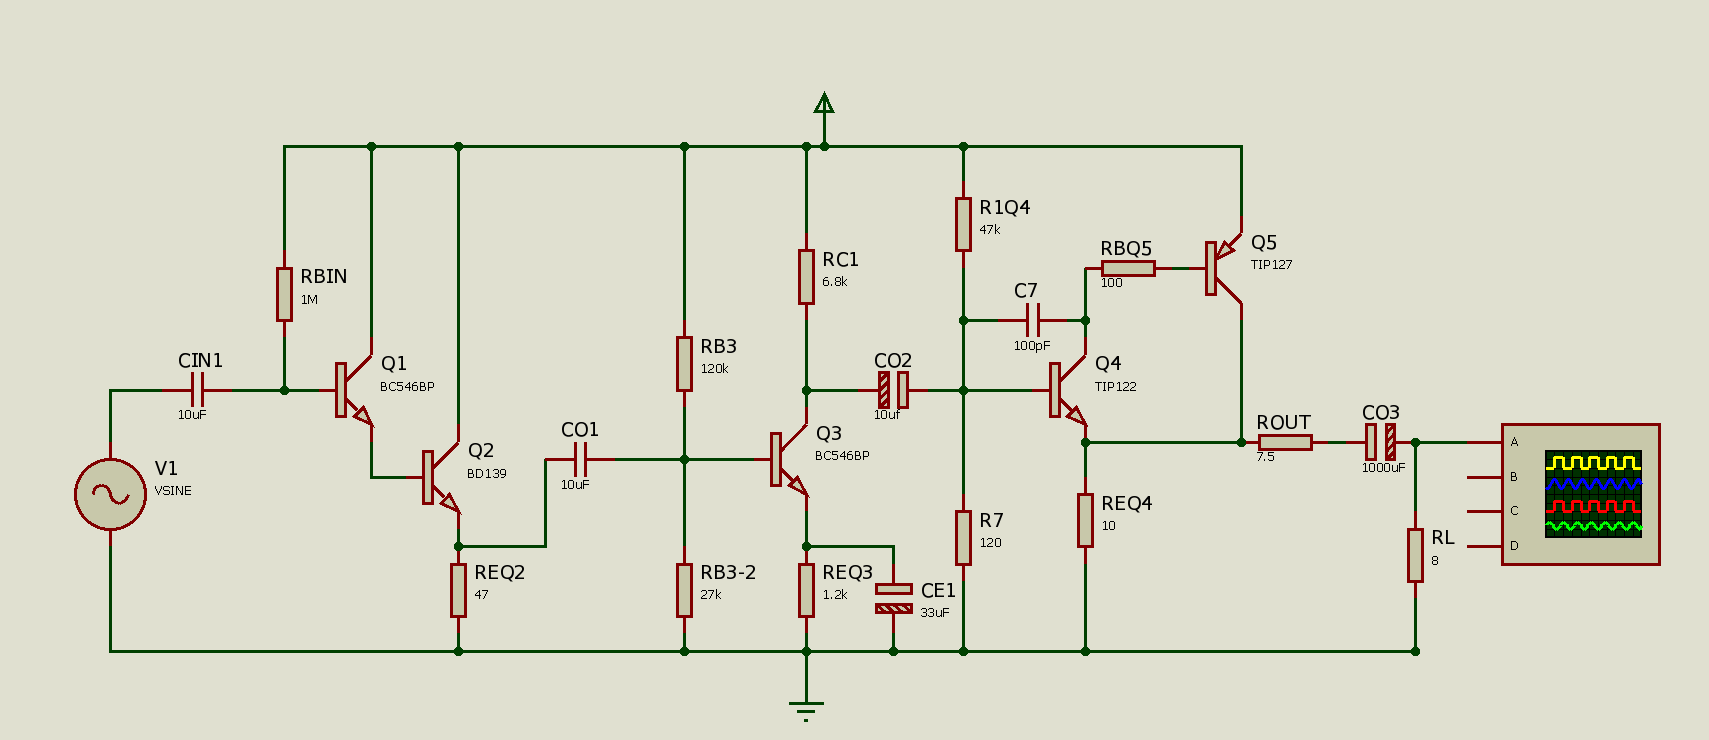
\includegraphics[width=\textwidth]{SetupMediciones/TensionesCorrientes/BarridoDeFrecuencia.png} % Ajusta el ancho al de la minipage
        \caption{Representacion esquematica.}
        \label{fig:esquematicoBarCompleto}
    \end{minipage}
    \hfill % Relleno elástico para separar las imágenes
    % Segunda minipage (ocupa el 45% del ancho de la página)
    \begin{minipage}{0.45\textwidth}
        \centering
        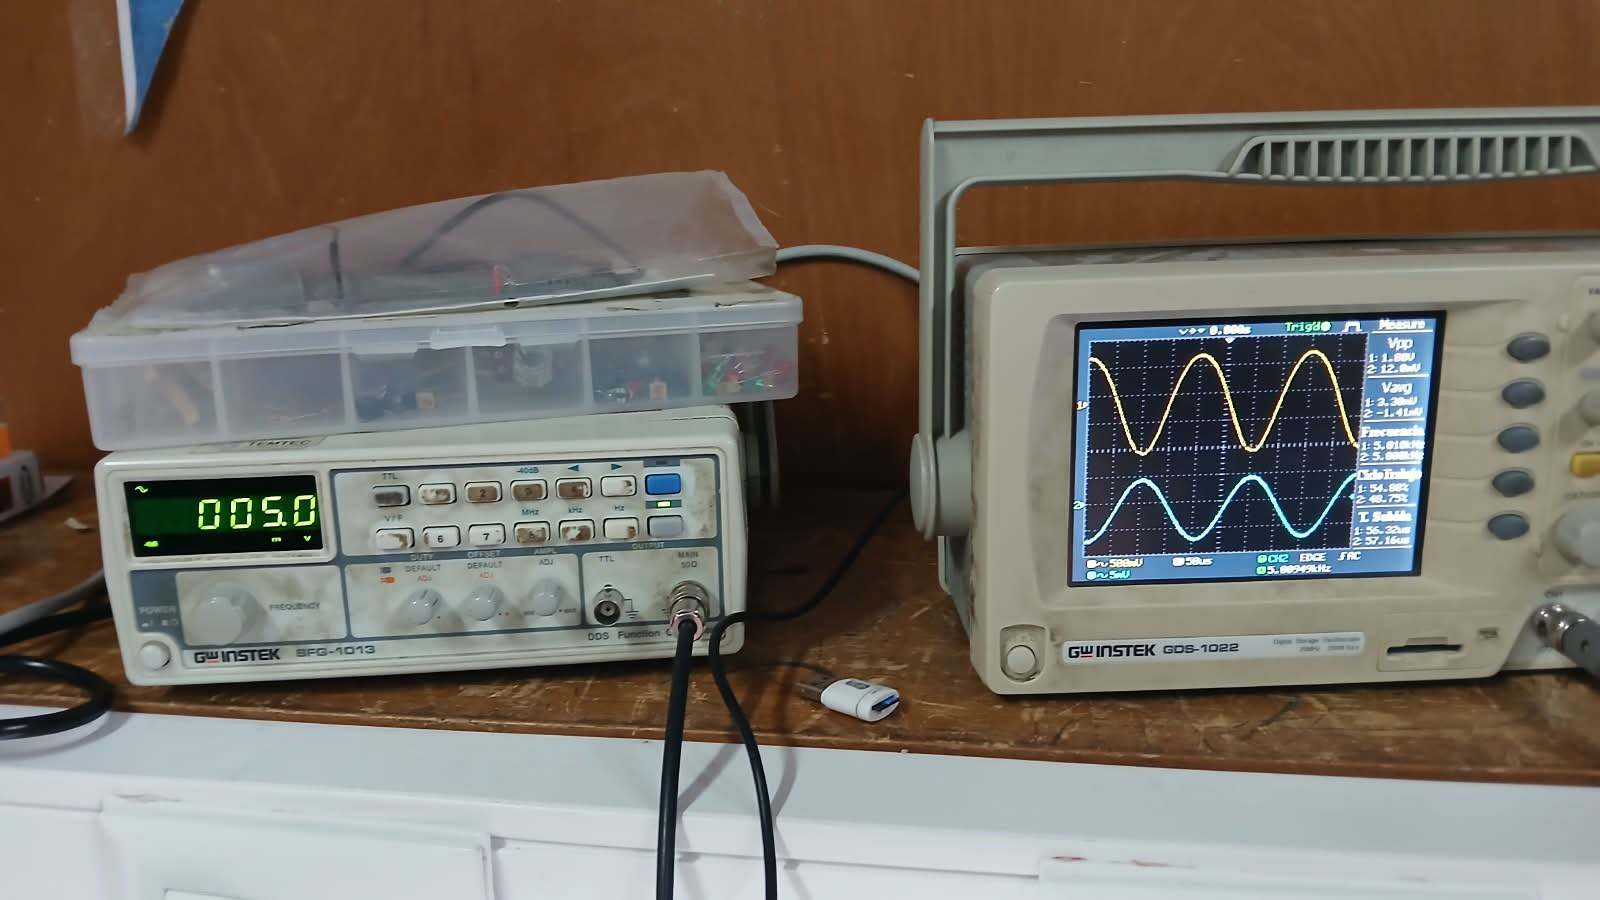
\includegraphics[width=\textwidth]{FotosMed/Barrido de amplitud/ETOTAL/5m.jpeg}
        \caption{Imagen de la Medición.}
        \label{fig:medicionBArCompleto}
    \end{minipage}
\end{figure}

\begin{figure}[H]
    \centering
    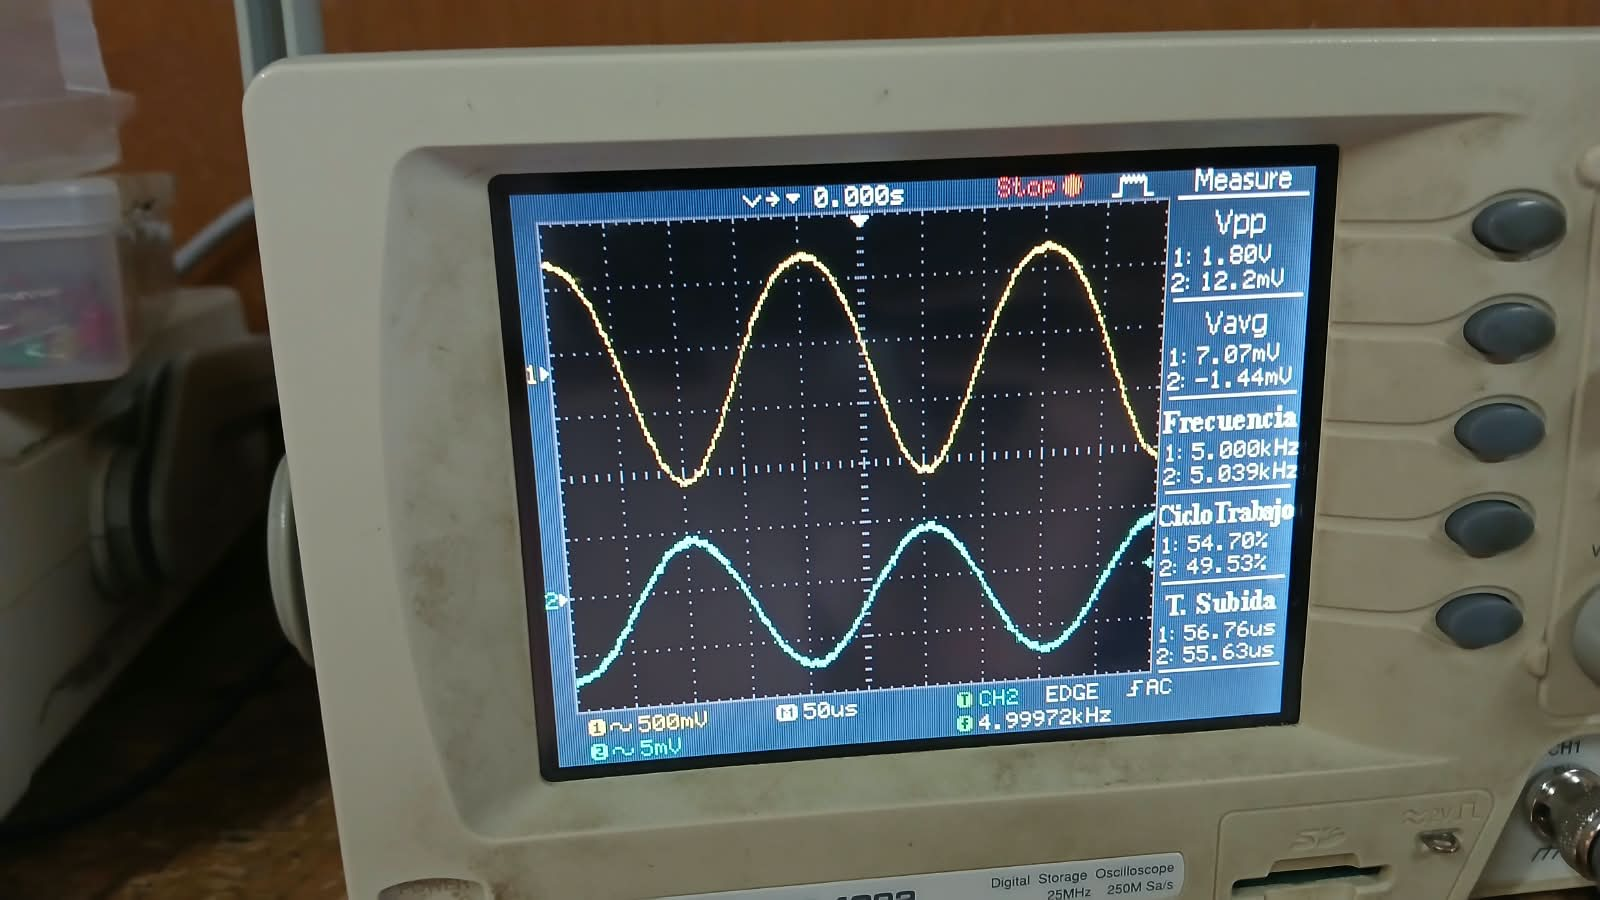
\includegraphics[width=0.8\textwidth]{FotosMed/Barrido de amplitud/ETOTAL/5mzoom.jpeg}
    \caption{Pantalla del Osciloscopio}
    \label{fig:osciloscopioBarCompleto}
\end{figure}

Se puede ver en \ref{fig:osciloscopioBarCompleto}, la tension de entrada esta en el canal 2 del osciloscopio(estipulada a 13.8 mV pico a pico) mientras que la salida se observa en el canal 1.

\subsection{Barrido de Frecuencia}
Realizada puramente observando el osciloscopio, se fue variando la frecuencia de salida del generador de decada en decada a medida que se realizaaban los calculos de ganancia, la amplitud de entrada fue establecida en 5,1 mV pico a pico.

Estas fueron realizadas en 3 configuraciones:
- Etapa 1 (Darlington)
- Etapa 1 y 2
- Circuito Completo

\subsubsection{Barrido de Etapa 1}
Utilizando la punta compensada conectada al osciloscopio se evaluó la tensión de salida de la primer etapa y se realizo el calculo de ganancia.

\begin{figure}[H]
    \centering
    % Primera minipage (ocupa el 45% del ancho de la página)
    \begin{minipage}{0.45\textwidth}
        \centering
        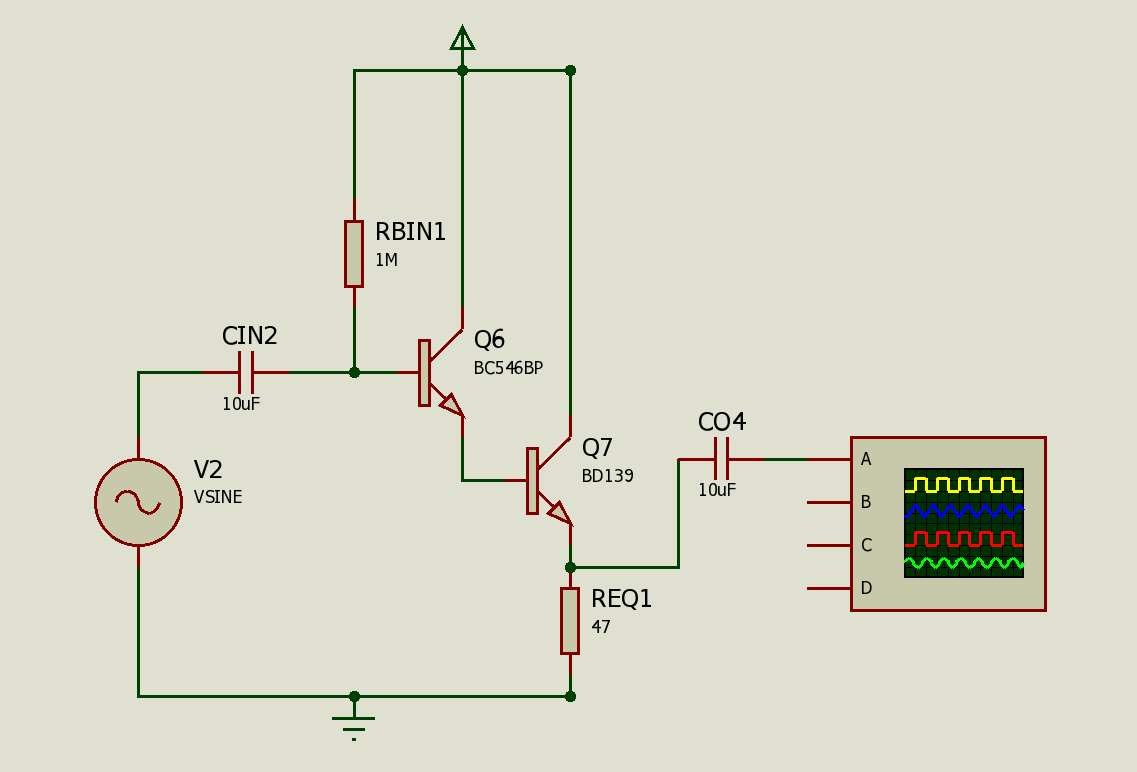
\includegraphics[width=\textwidth]{SetupMediciones/ZOUT/ZoutDARSinCarga.png} % Ajusta el ancho al de la minipage
        \caption{Representacion esquematica.}
        \label{fig:esquematicoBarFrec}
    \end{minipage}
    \hfill % Relleno elástico para separar las imágenes
    % Segunda minipage (ocupa el 45% del ancho de la página)
    \begin{minipage}{0.45\textwidth}
        \centering
        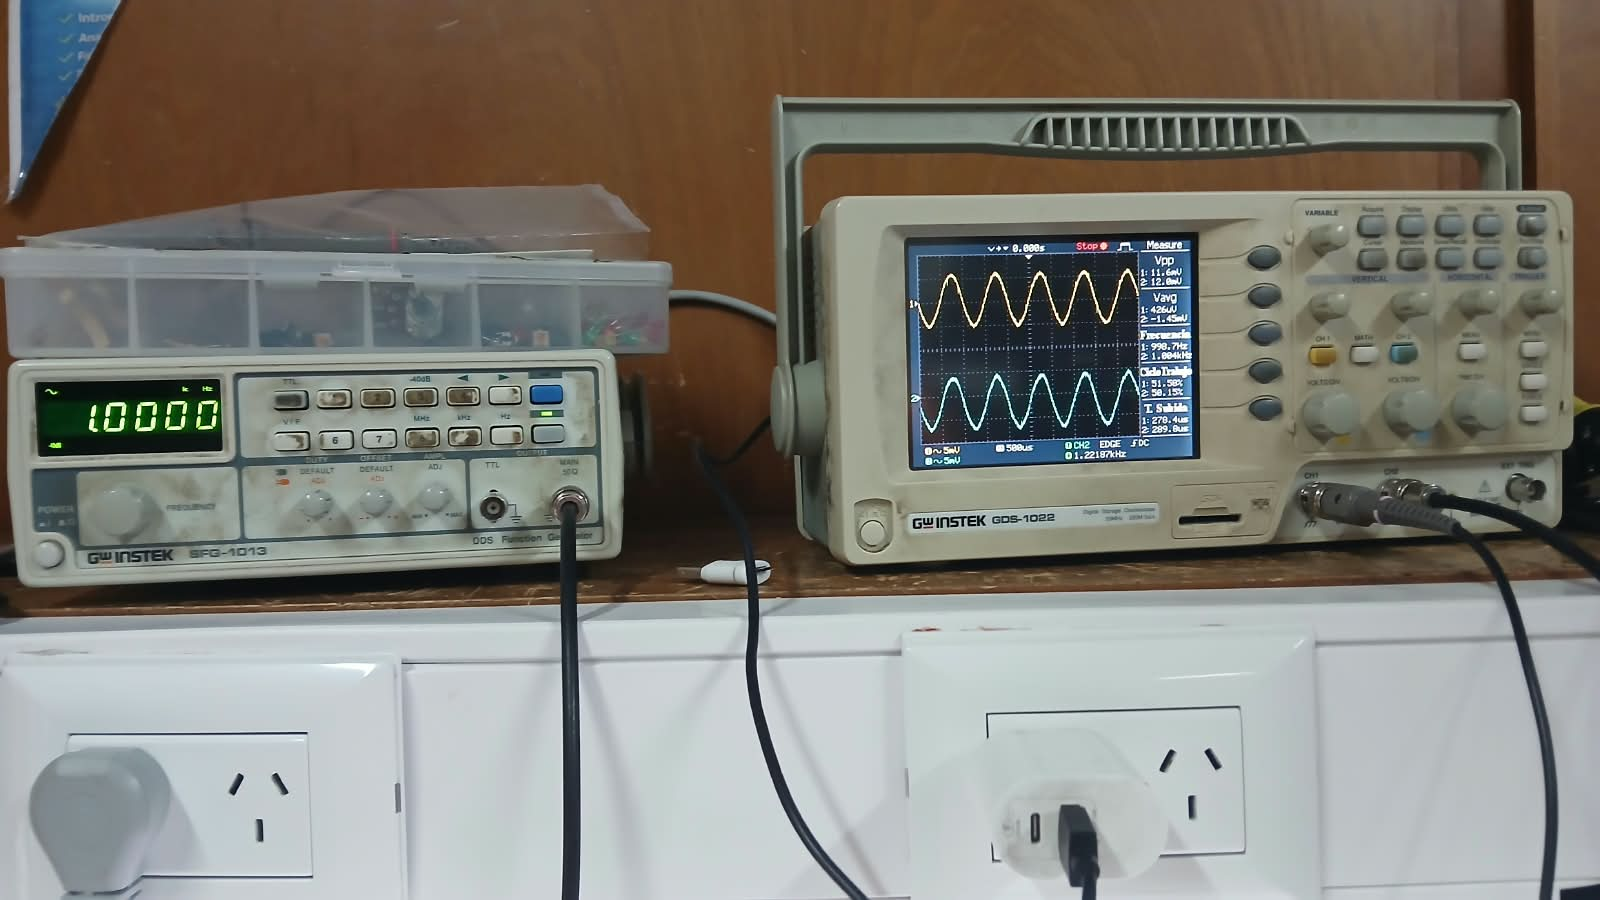
\includegraphics[width=\textwidth]{FotosMed/Barrido de frecuencia/E1/1k.jpeg}
        \caption{Imagen de la Medicion.}
        \label{fig:medicionBarFrec}
    \end{minipage}
\end{figure}

\begin{figure}[H]
    \centering
    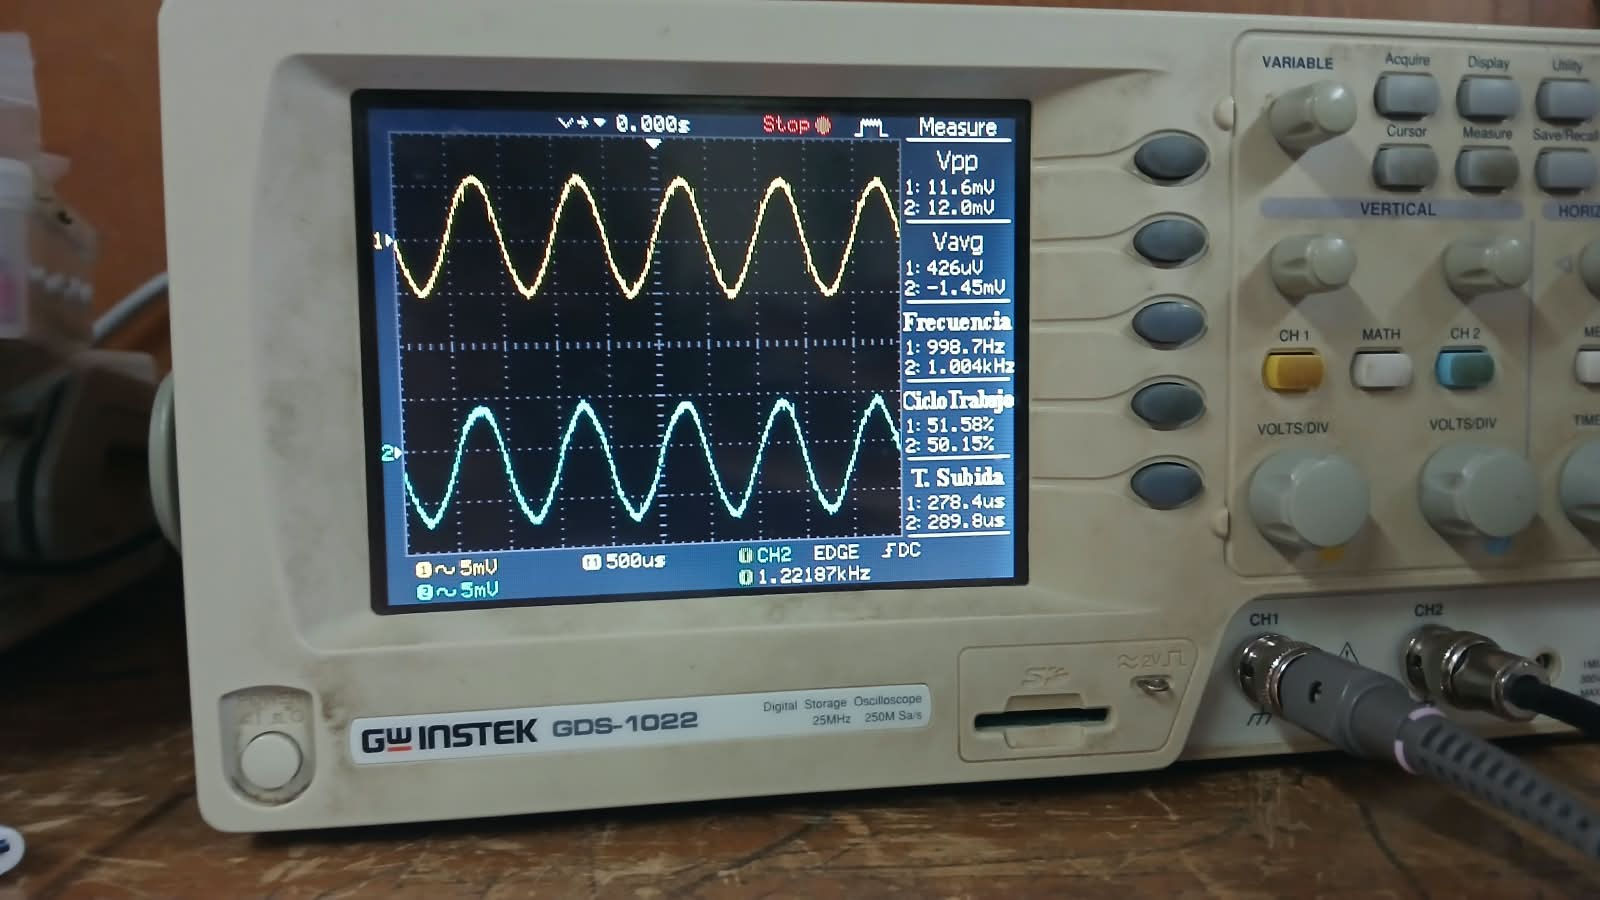
\includegraphics[width=0.8\textwidth]{FotosMed/Barrido de frecuencia/E1/1kzoom.jpeg}
    \caption{Pantalla del Osciloscopio}
    \label{fig:osciloscopioBArFrec}
\end{figure}

Se puede ver en \ref{fig:osciloscopioBArFrec}, la tension de entrada esta en el canal 2 del osciloscopio mientras que la salida se observa en el canal 1. El comportamiento es el esperado.

\subsubsection{Barrido de Etapa 1 y 2}
Al igual que con la medicion anterior y en la proxima, se uso la punta compensada conectada al osciloscopio para obtener las mediciones de tension

\begin{figure}[H]
    \centering
    % Primera minipage (ocupa el 45% del ancho de la página)
    \begin{minipage}{0.45\textwidth}
        \centering
        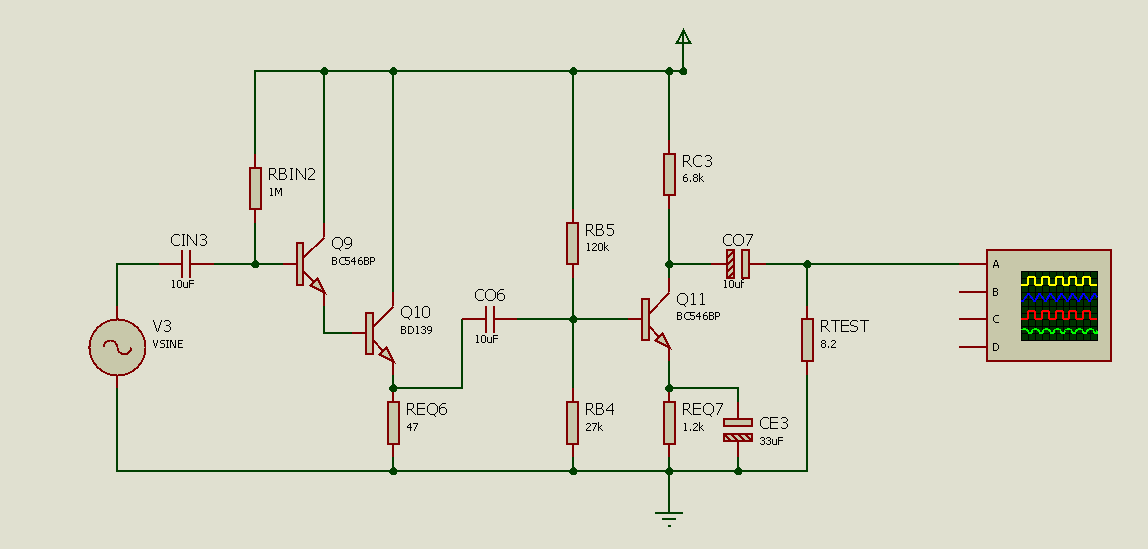
\includegraphics[width=\textwidth]{SetupMediciones/ZOUT/Zout12Cargada.png} % Ajusta el ancho al de la minipage
        \caption{Representacion esquematica.}
        \label{fig:esquematicofrec12}
    \end{minipage}
    \hfill % Relleno elástico para separar las imágenes
    % Segunda minipage (ocupa el 45% del ancho de la página)
    \begin{minipage}{0.45\textwidth}
        \centering
        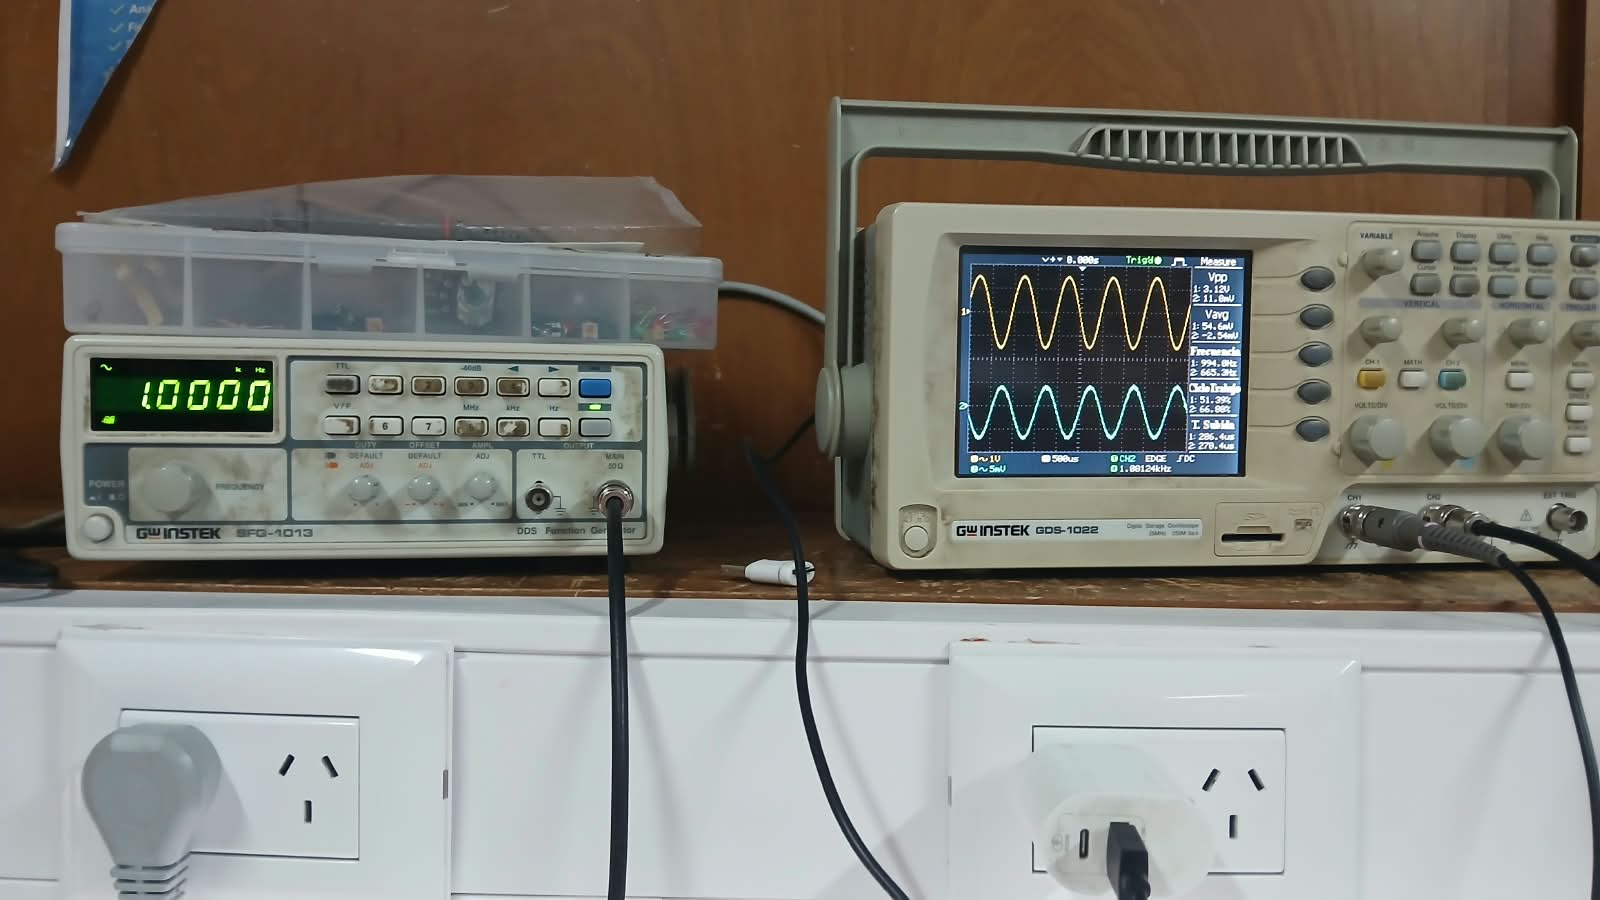
\includegraphics[width=\textwidth]{FotosMed/Barrido de frecuencia/E12/1k.jpeg}
        \caption{Imagen de la Medicion.}
        \label{fig:medicionfrec12}
    \end{minipage}
\end{figure}

\begin{figure}[H]
    \centering
    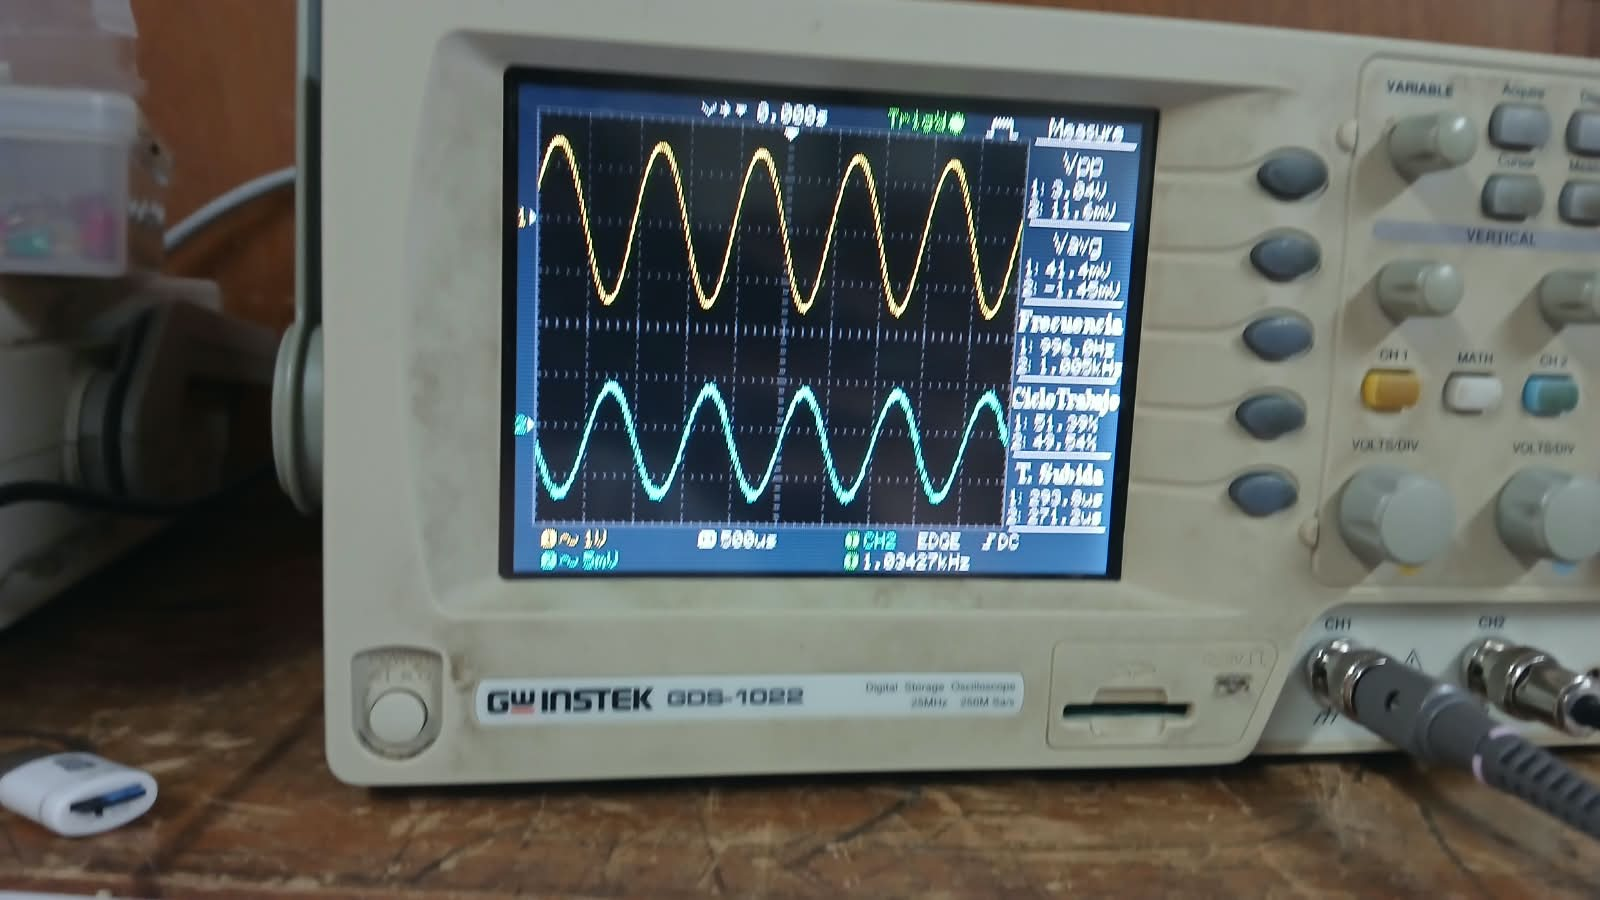
\includegraphics[width=0.8\textwidth]{FotosMed/Barrido de frecuencia/E12/1kzoom.jpeg}
    \caption{Pantalla del Osciloscopio}
    \label{fig:osciloscopiofrec12}
\end{figure}

Se puede ver en \ref{fig:osciloscopiofrec12} que la entrada esta conectada al canal 2 mientras que la salida al Canal 1, en estas etapas ya se evidencia la contundente ganancia.

\subsubsection{Barrido en circuito completo}
Sin casi variaciones, la medicion es reaizada observando la salida del circuito completo.

\begin{figure}[H]
    \centering
    % Primera minipage (ocupa el 45% del ancho de la página)
    \begin{minipage}{0.45\textwidth}
        \centering
        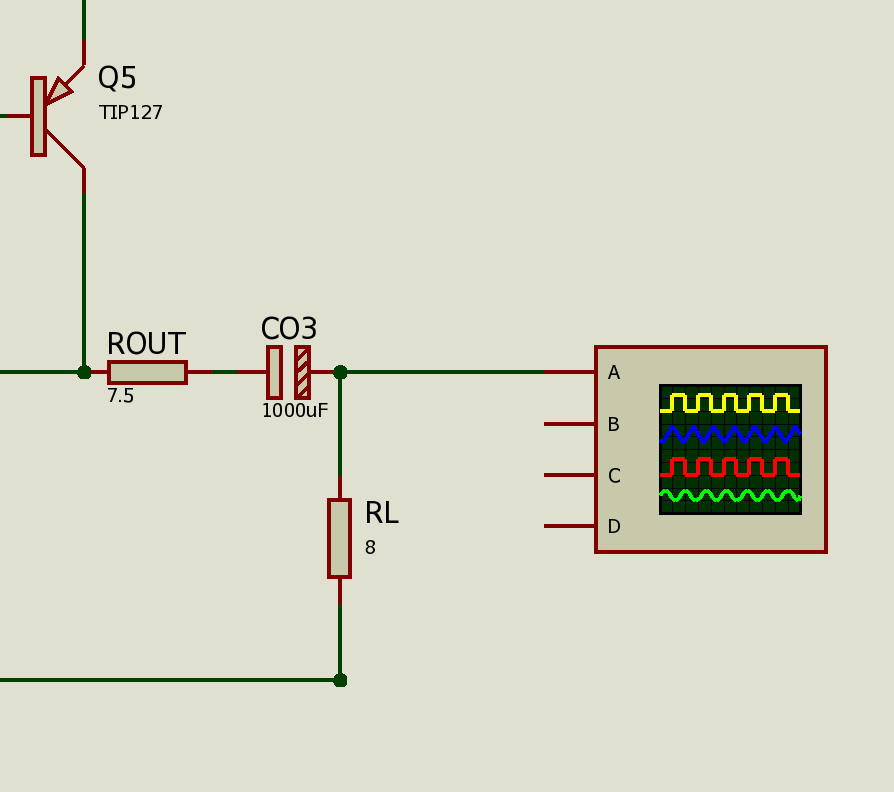
\includegraphics[width=\textwidth]{SetupMediciones/ZOUT/ZoutCarga.png} % Ajusta el ancho al de la minipage
        \caption{Representacion esquematica.}
        \label{fig:esquematicofrectotal}
    \end{minipage}
    \hfill % Relleno elástico para separar las imágenes
    % Segunda minipage (ocupa el 45% del ancho de la página)
    \begin{minipage}{0.45\textwidth}
        \centering
        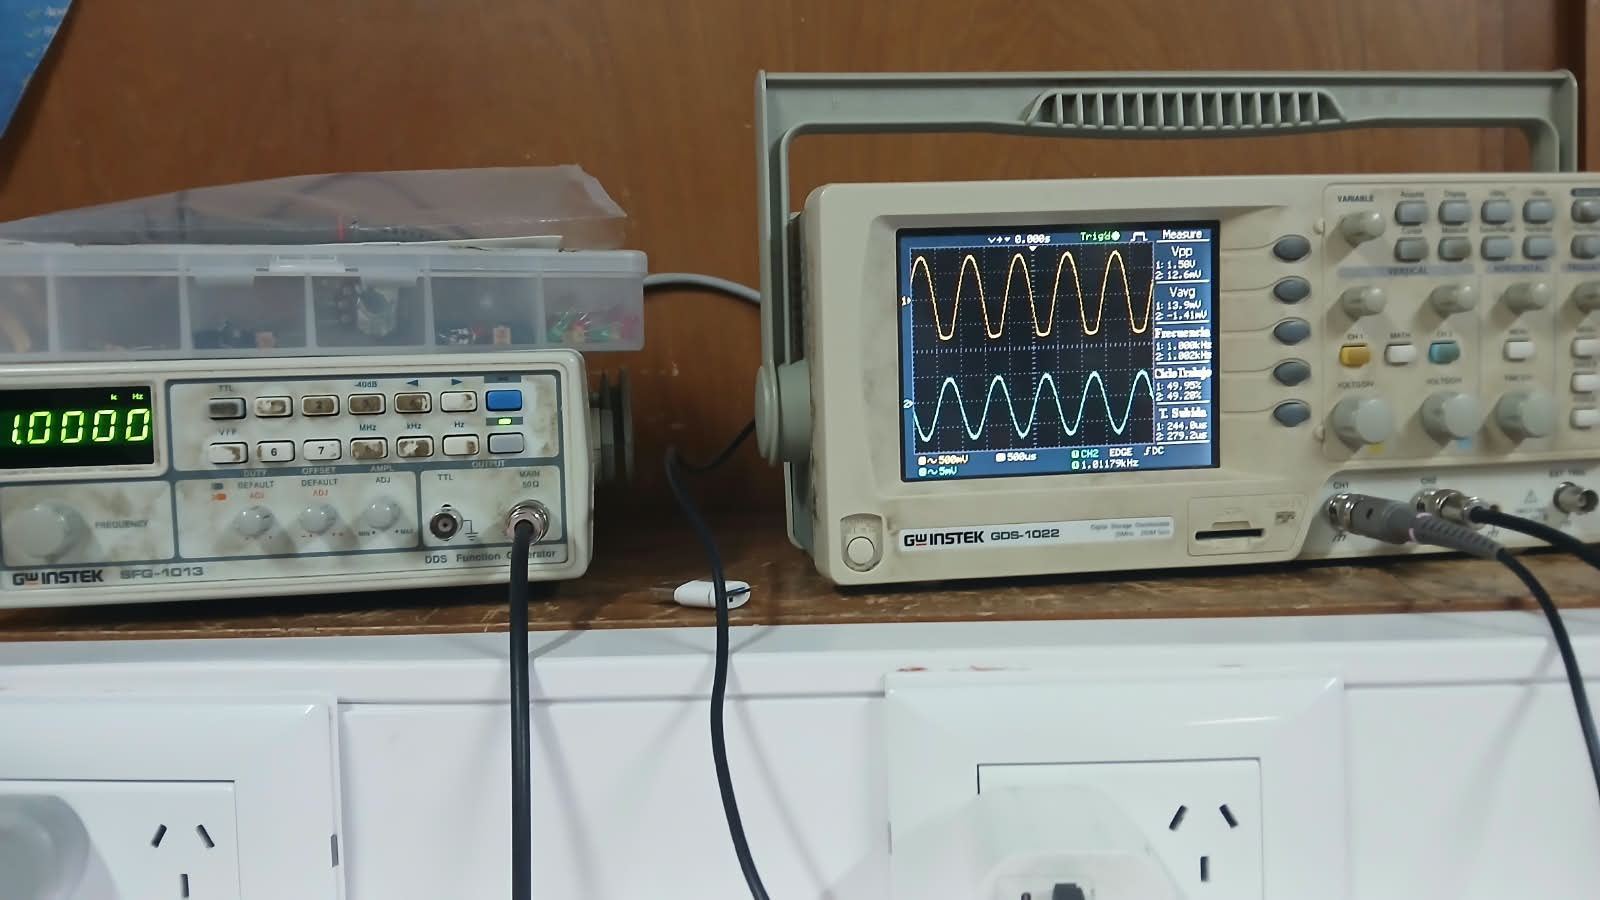
\includegraphics[width=\textwidth]{FotosMed/Barrido de frecuencia/Completo/1khz.jpeg}
        \caption{Imagen de la Medicion.}
        \label{fig:medicionfrectotal}
    \end{minipage}
\end{figure}

\begin{figure}[H]
    \centering
    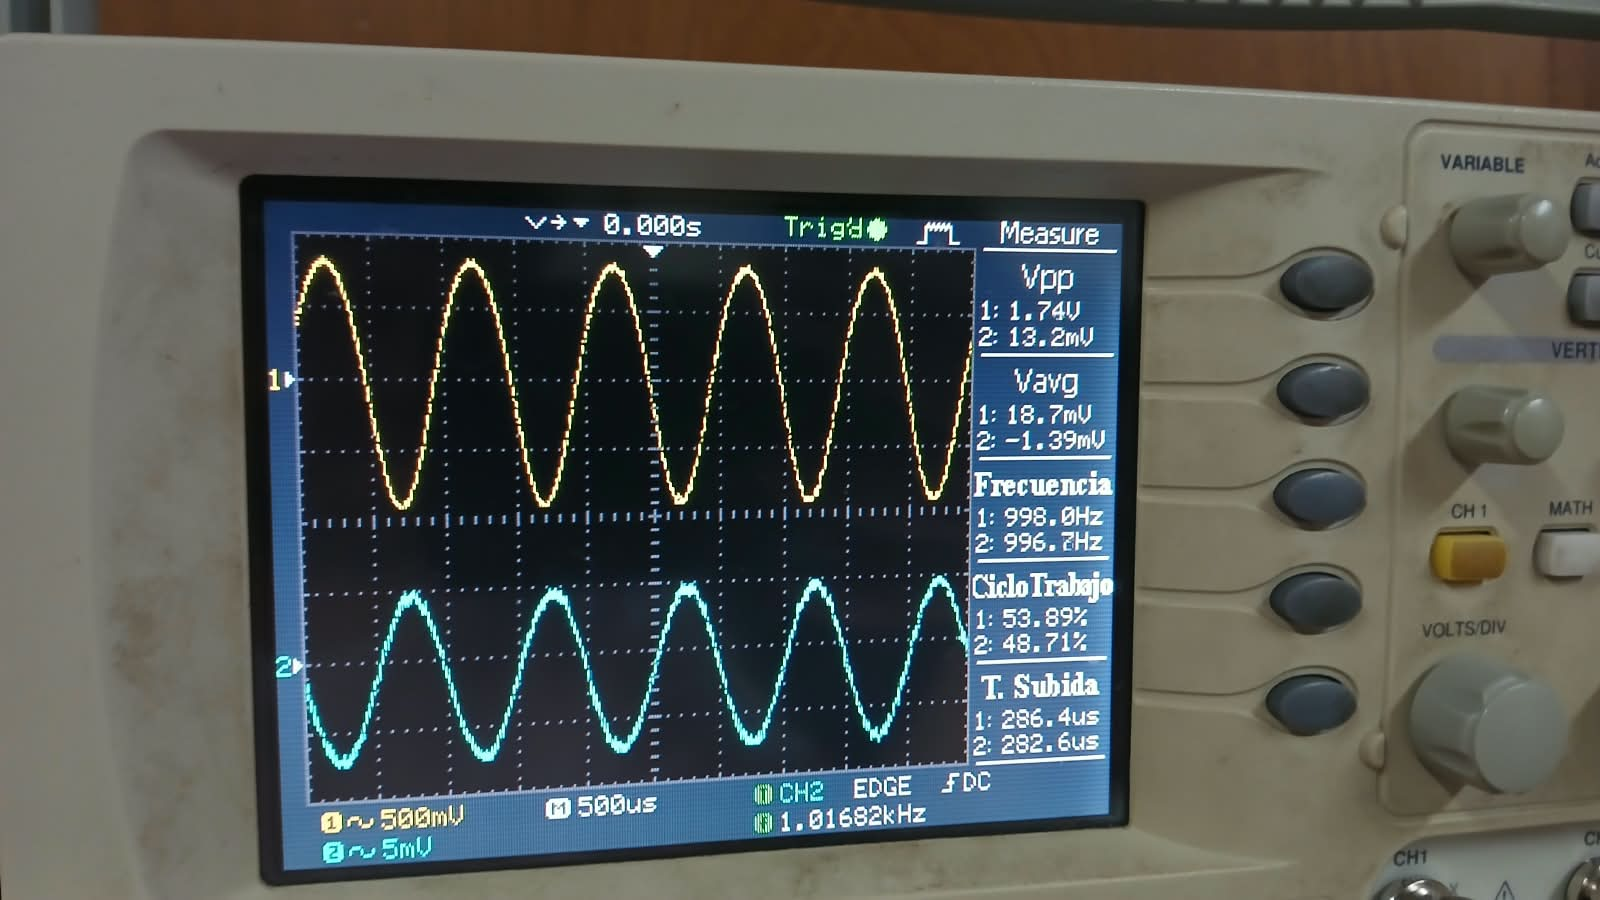
\includegraphics[width=0.8\textwidth]{FotosMed/Barrido de frecuencia/Completo/1khzzoom.jpeg}
    \caption{Pantalla del Osciloscopio}
    \label{fig:osciloscopiofrectotal}
\end{figure}

Se puede ver en \ref{fig:osciloscopiofrectotal} que la entrada esta conectada al canal 2 mientras que la salida al Canal 1, la ganancia disminuyo a la mitad en comparacion a la medicion anterior.

\subsection{Total Harmonic Distorsion}
Con la misma distribucion dada en el barrido de frecuencia, en este caso se utilizó la funcion de obtener la Transformada Rapida de Fourier (FFT) del osciloscopio para realizar los calculos de THD mediante:

\[
\mathrm{THD} = \frac{\sqrt{V_2^2 + V_3^2 + V_4^2 + \cdots + V_n^2}}{V_1}
\]

Como se dijo anteriormente, se midio en
- Etapa 1(Darlington)
- Etapa 1 y 2
- Circuito Completo

\subsubsection{FFT de Etapa 1}
Utilizando la punta compensada conectada al osciloscopio se obtuvo la salida de la etapa 1 y se aplico la FFT, una vez impresa en la pantalla se realizaron los calculos pertientes para determinar la THD.

\begin{figure}[H]
    \centering
    % Primera minipage (ocupa el 45% del ancho de la página)
    \begin{minipage}{0.45\textwidth}
        \centering
        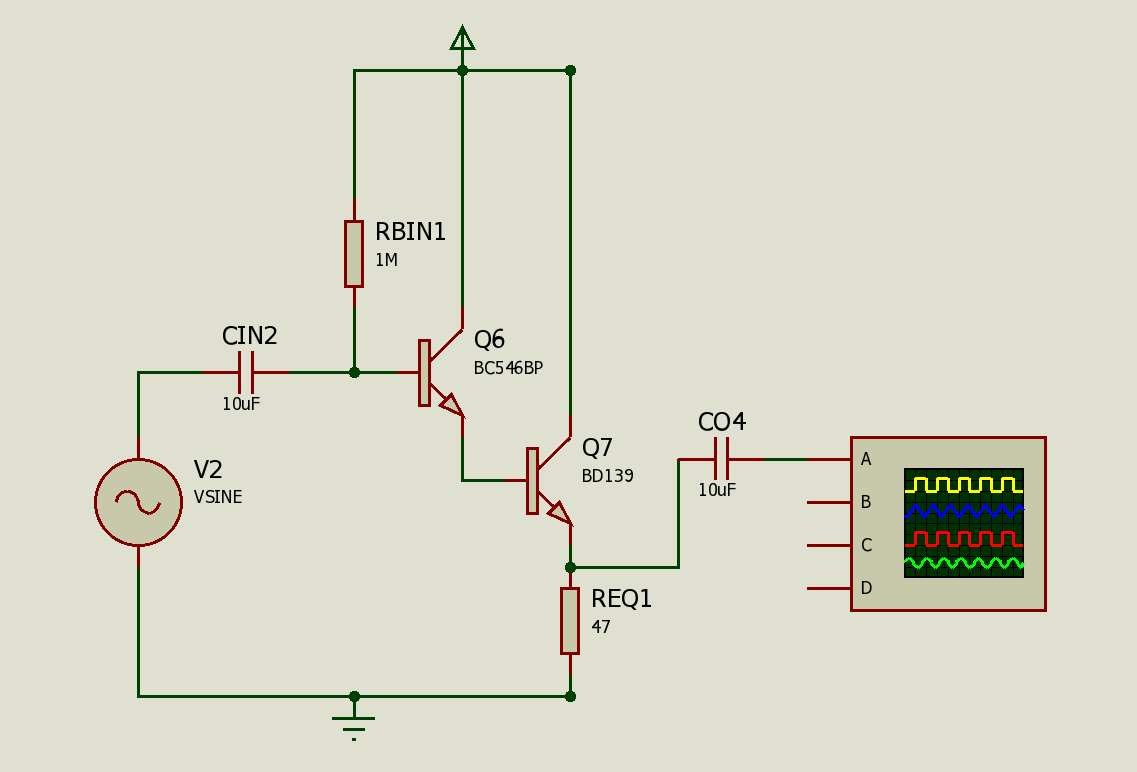
\includegraphics[width=\textwidth]{SetupMediciones/ZOUT/ZoutDARSinCarga.png} % Ajusta el ancho al de la minipage
        \caption{Representacion esquematica.}
        \label{fig:esquematicoFFT1}
    \end{minipage}
    \hfill % Relleno elástico para separar las imágenes
    % Segunda minipage (ocupa el 45% del ancho de la página)
    \begin{minipage}{0.45\textwidth}
        \centering
        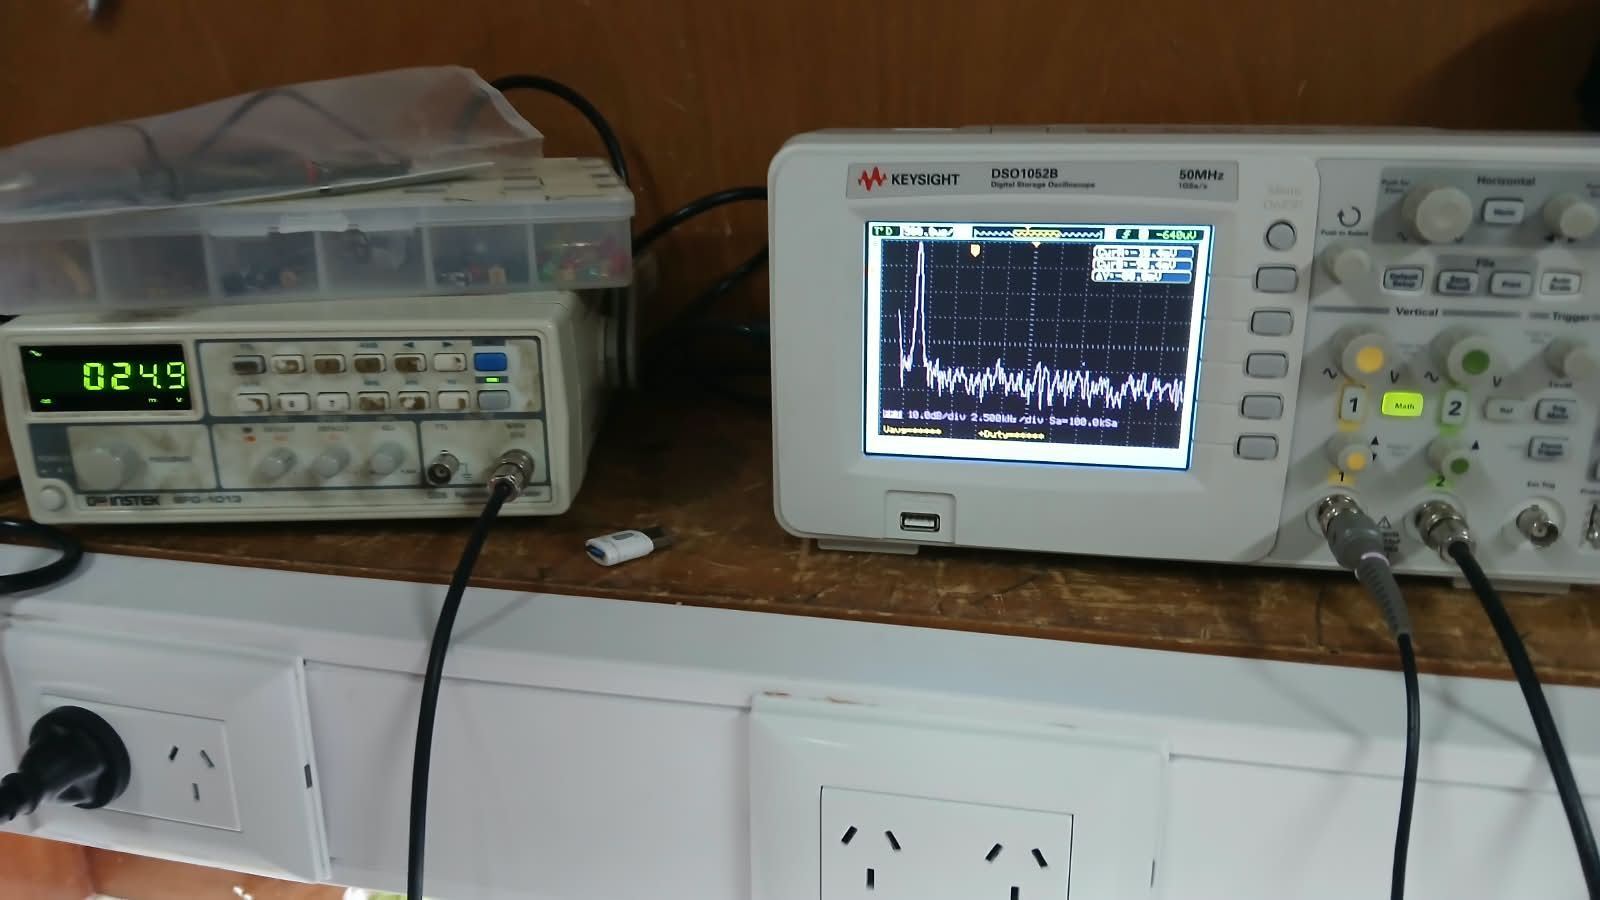
\includegraphics[width=\textwidth]{FotosMed/FFT/Dar/25dar.jpeg}
        \caption{Imagen de la Medicion.}
        \label{fig:medicionFFT1}
    \end{minipage}
\end{figure}

\begin{figure}[H]
    \centering
    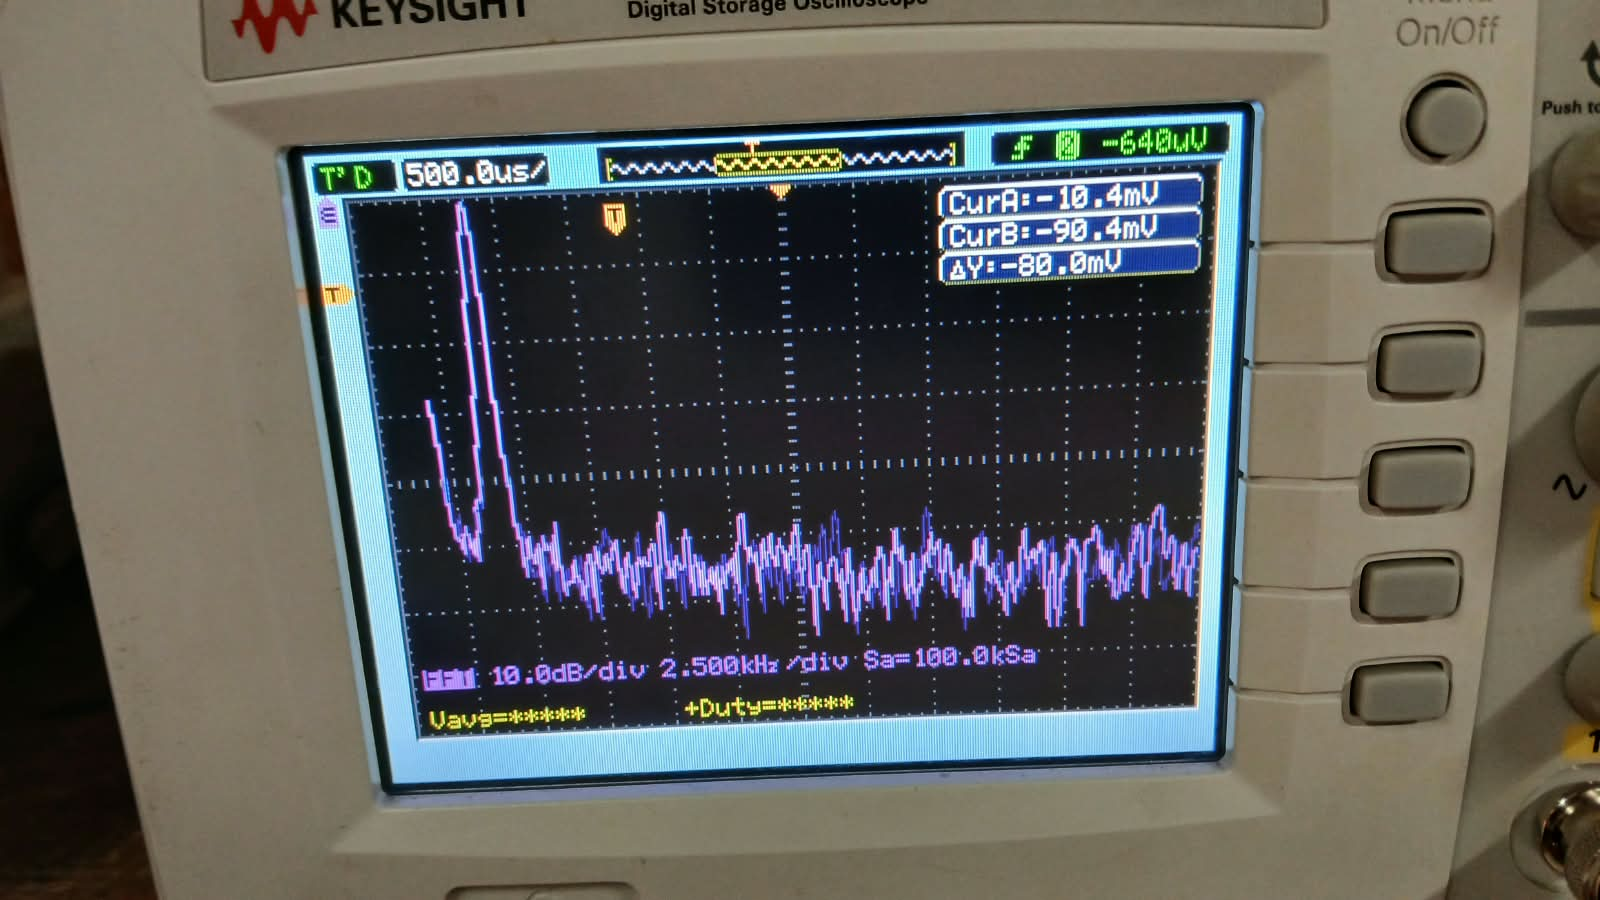
\includegraphics[width=0.8\textwidth]{FotosMed/FFT/Dar/25darzoom.jpeg}
    \caption{Pantalla del Osciloscopio}
    \label{fig:osciloscopioFFT1}
\end{figure}

Se puede ver en la Figura \ref{fig:osciloscopioFFT1}, la de entrada esta en el canal 2 del osciloscopio mientras que la salida se observa en el canal 1.No se observa casi distorsion en esta primer etapa.

\subsubsection{Barrido de Etapa 1 y 2}
Aqui se conectan los jumpers necesarios y se cambia la posicion de la punta a la salida de la etapa 2.

\begin{figure}[h]
    \centering
    % Primera minipage (ocupa el 45% del ancho de la página)
    \begin{minipage}{0.45\textwidth}
        \centering
        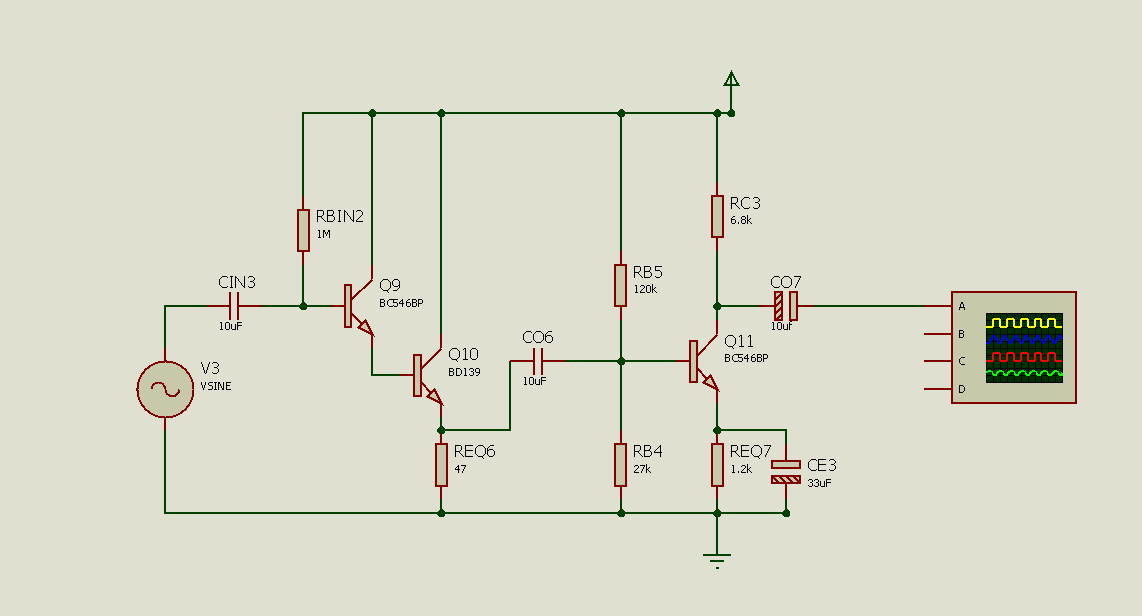
\includegraphics[width=\textwidth]{SetupMediciones/ZOUT/Zout12VACIO.png} % Ajusta el ancho al de la minipage
        \caption{Representacion esquematica.}
        \label{fig:esquematicpFFT12}
    \end{minipage}
    \hfill % Relleno elástico para separar las imágenes
    % Segunda minipage (ocupa el 45% del ancho de la página)
    \begin{minipage}{0.45\textwidth}
        \centering
        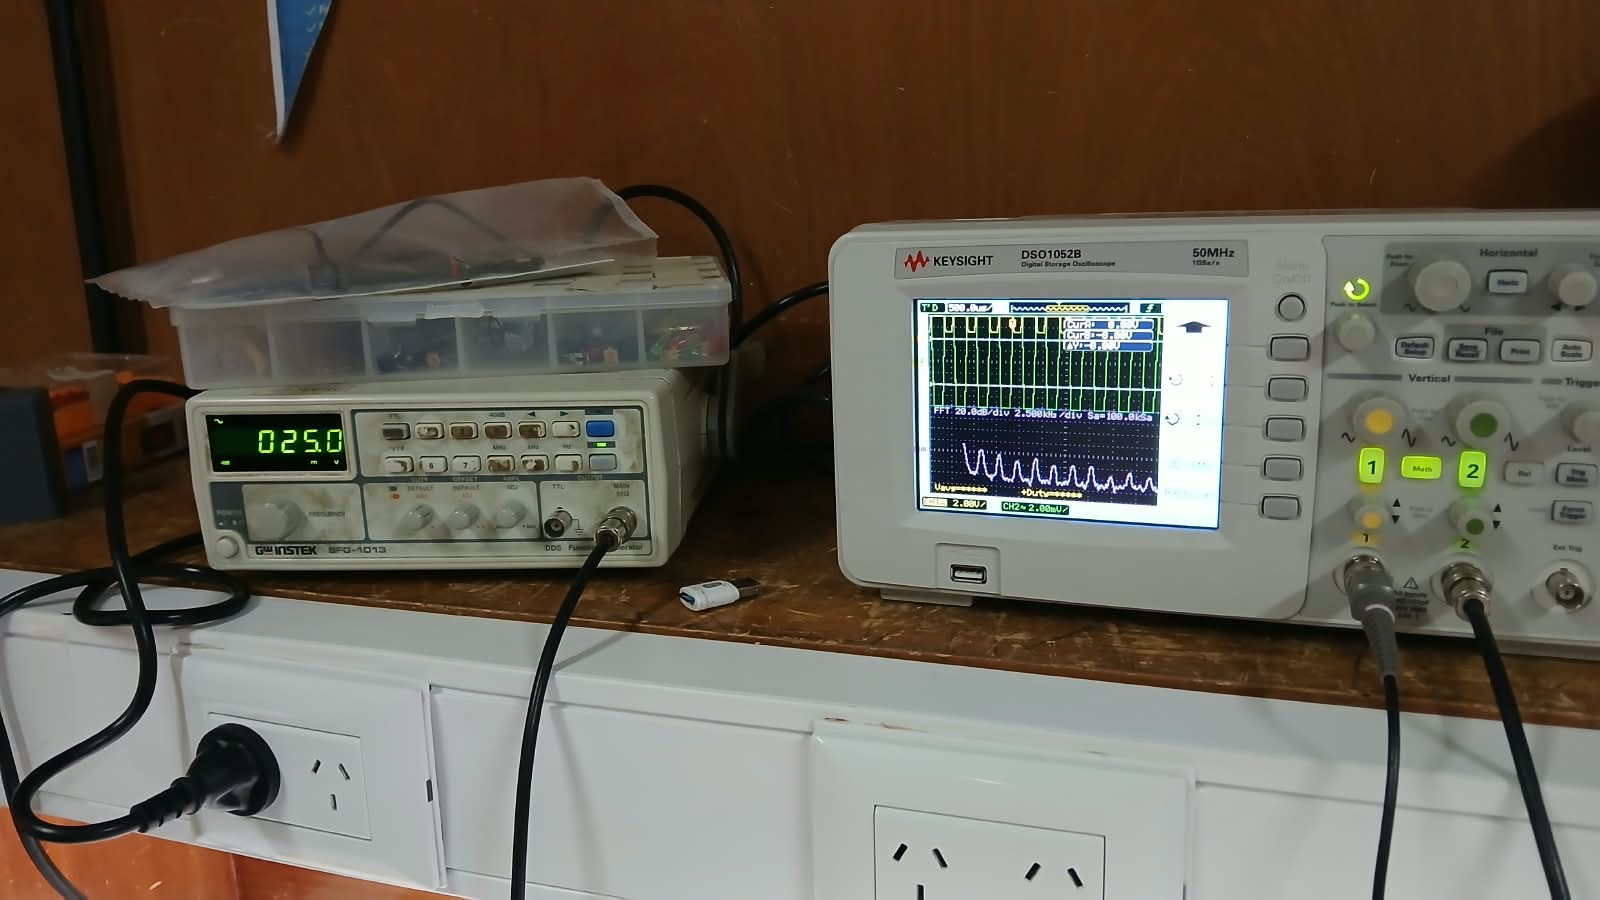
\includegraphics[width=\textwidth]{FotosMed/FFT/E12/25e12.jpeg}
        \caption{Imagen de la Medicion.}
        \label{fig:medicionFFT12}
    \end{minipage}
\end{figure}

\begin{figure}[H]
    \centering
    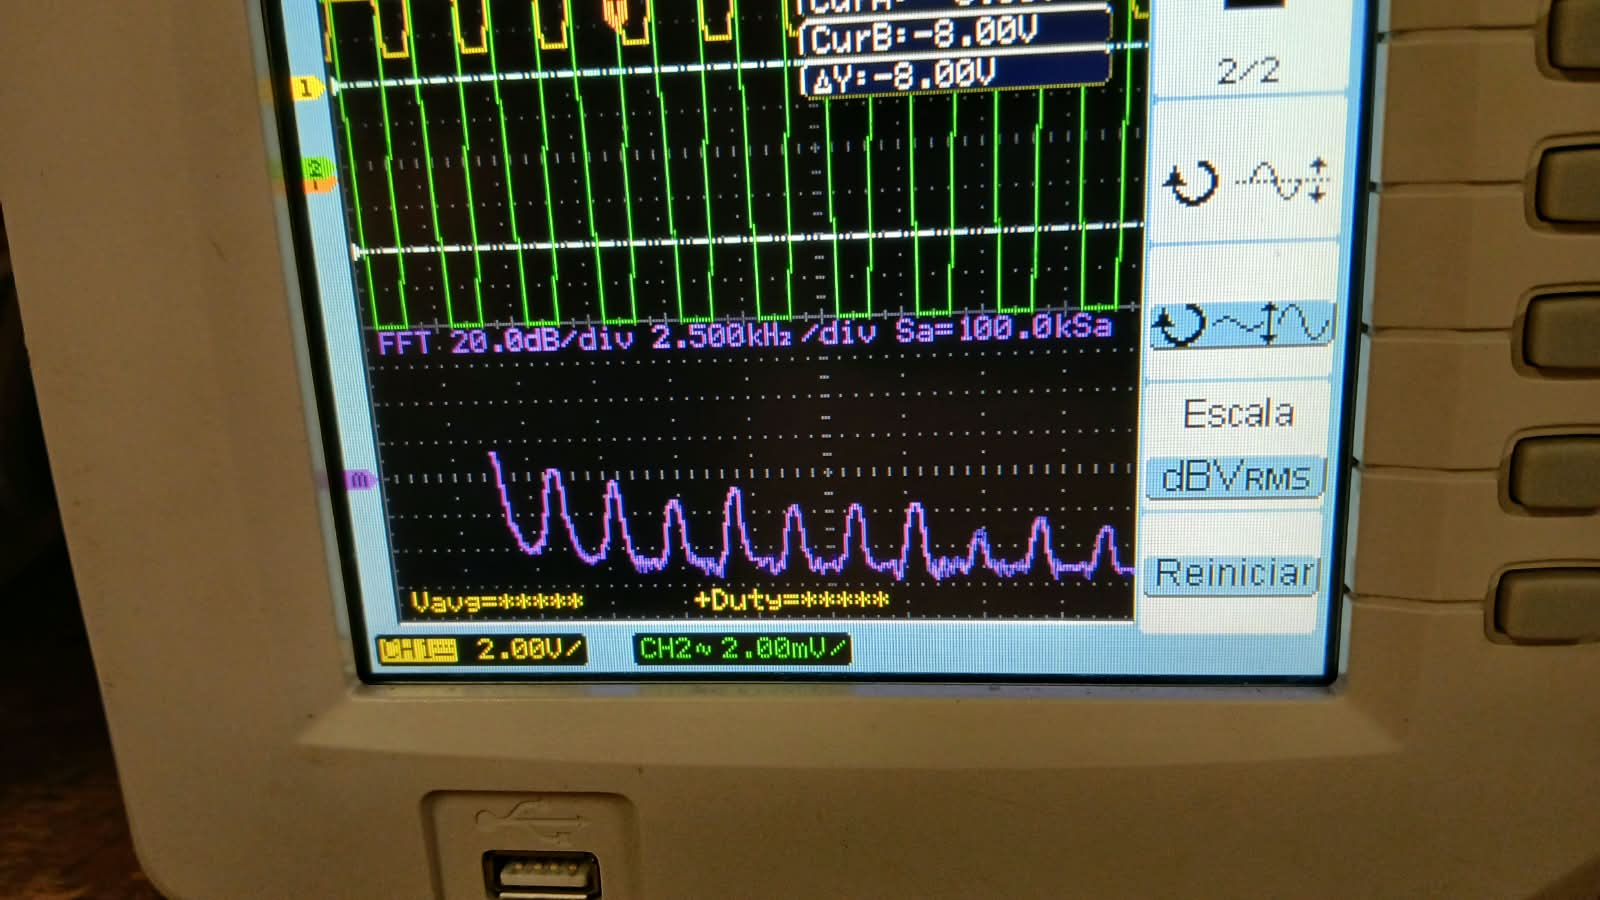
\includegraphics[width=0.8\textwidth]{FotosMed/FFT/E12/25e12zoom.jpeg}
    \caption{Pantalla del Osciloscopio}
    \label{fig:osciloscopioFFT12}
\end{figure}

Se puede ver en \ref{fig:osciloscopioFFT12} como la distorsión toma protagonismo evidenciandose en los picos de amplitud en frecuencias multiplos de 2Khz.

\subsubsection{FFT de circuito completo}
Con todos los jumpers conectados, se evalua la FFT del circuito final en la pantalla del osciloscopio 

\begin{figure}[H]
    \centering
    % Primera minipage (ocupa el 45% del ancho de la página)
    \begin{minipage}{0.45\textwidth}
        \centering
        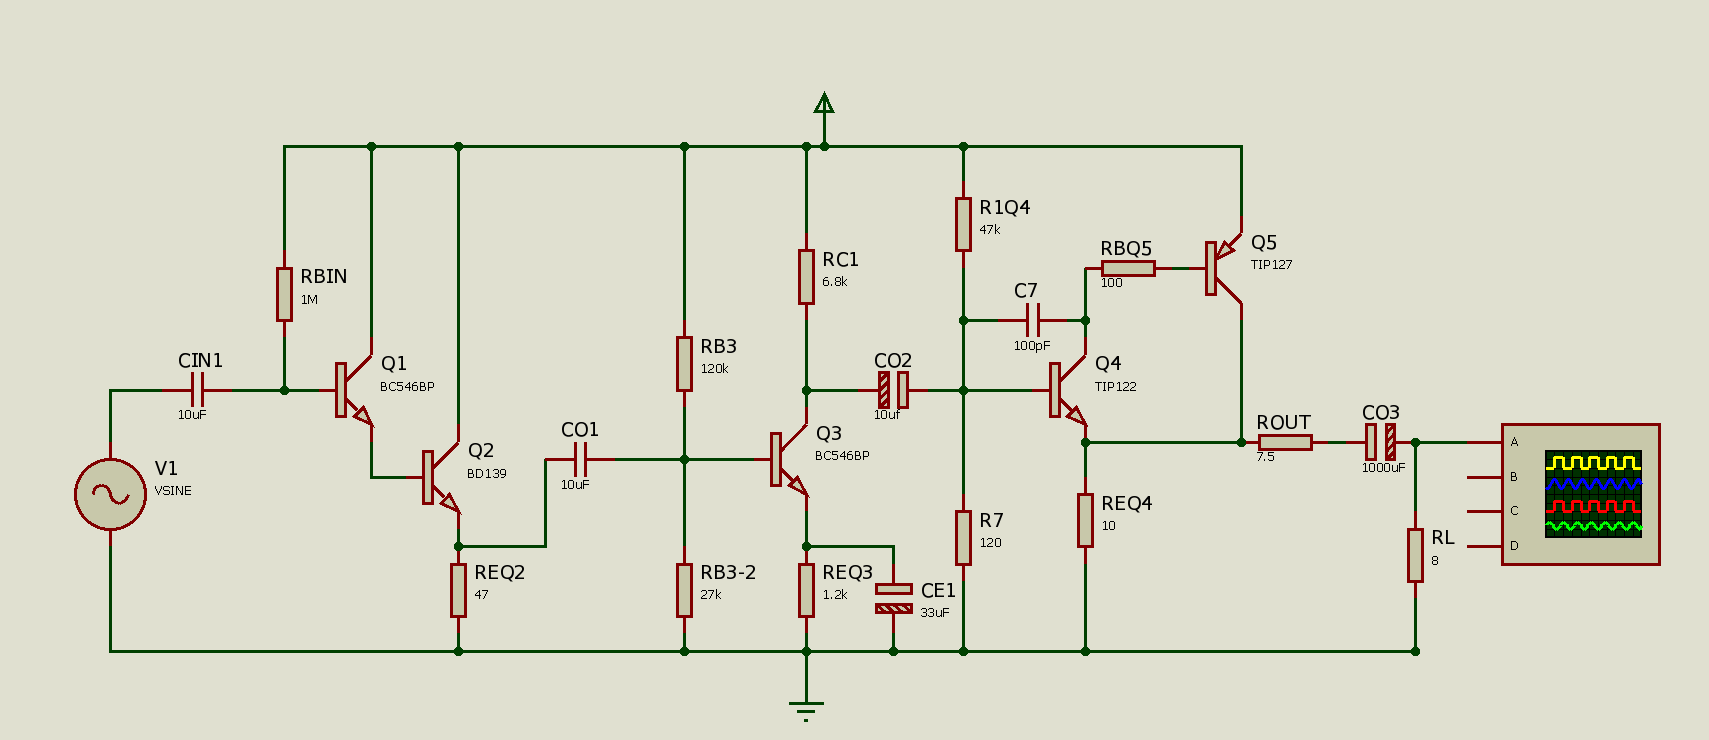
\includegraphics[width=\textwidth]{SetupMediciones/TensionesCorrientes/BarridoDeFrecuencia.png} % Ajusta el ancho al de la minipage
        \caption{Representacion esquematica.}
        \label{fig:esquematicoFFTCompleto}
    \end{minipage}
    \hfill % Relleno elástico para separar las imágenes
    % Segunda minipage (ocupa el 45% del ancho de la página)
    \begin{minipage}{0.45\textwidth}
        \centering
        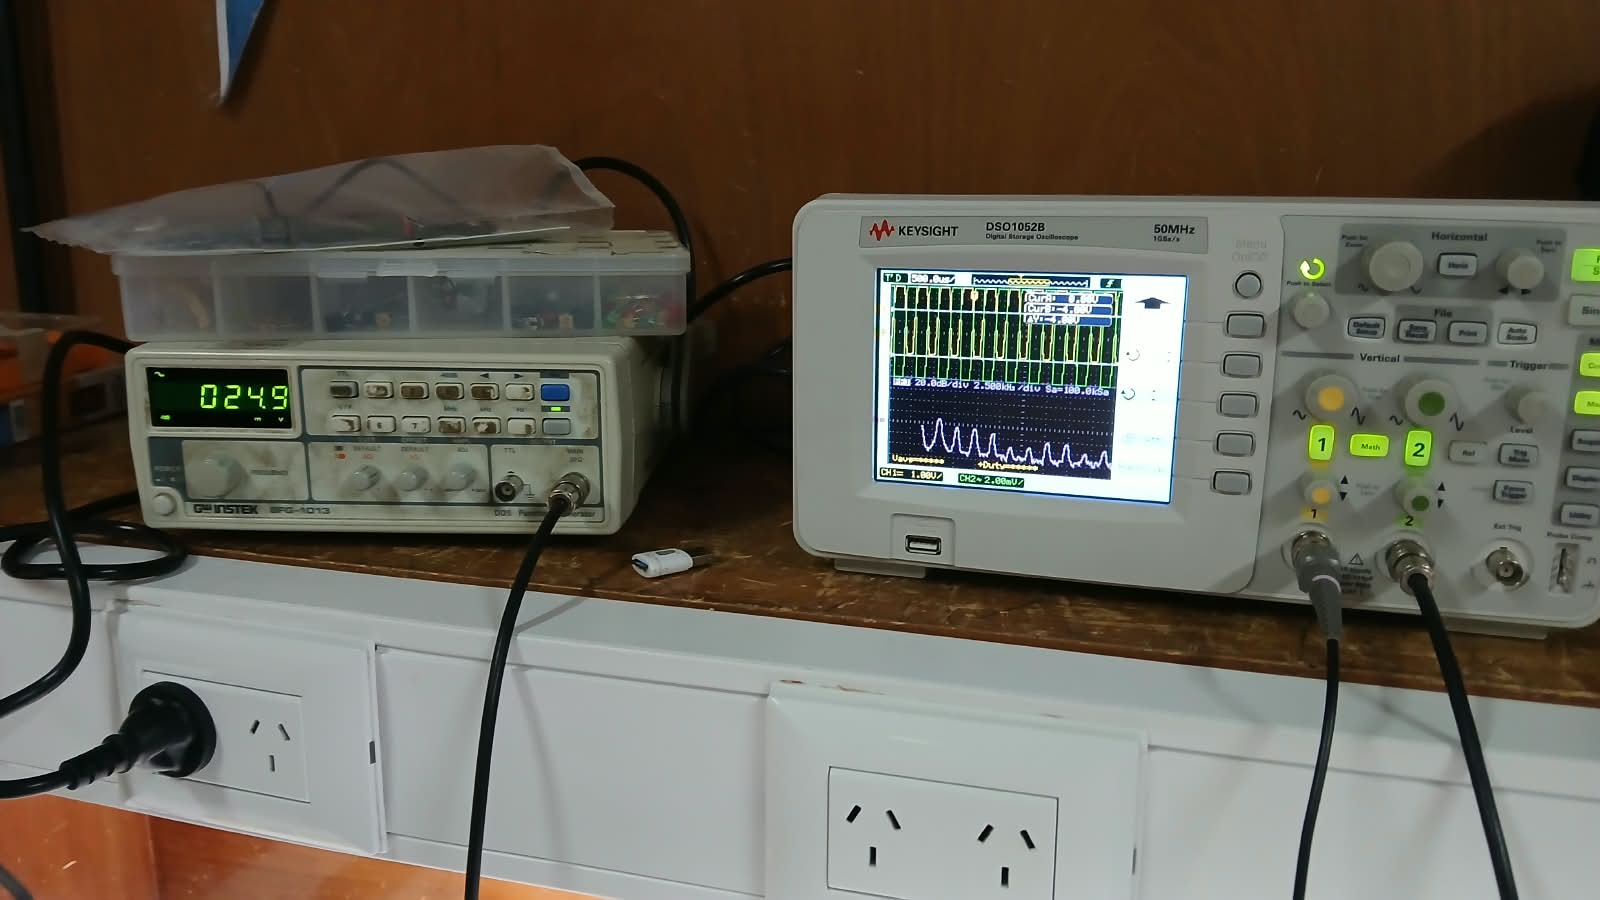
\includegraphics[width=\textwidth]{FotosMed/FFT/Completo/25com.jpeg}
        \caption{Imagen de la Medicion.}
        \label{fig:medicionFFTCompleto}
    \end{minipage}
\end{figure}

\begin{figure}[H]
    \centering
    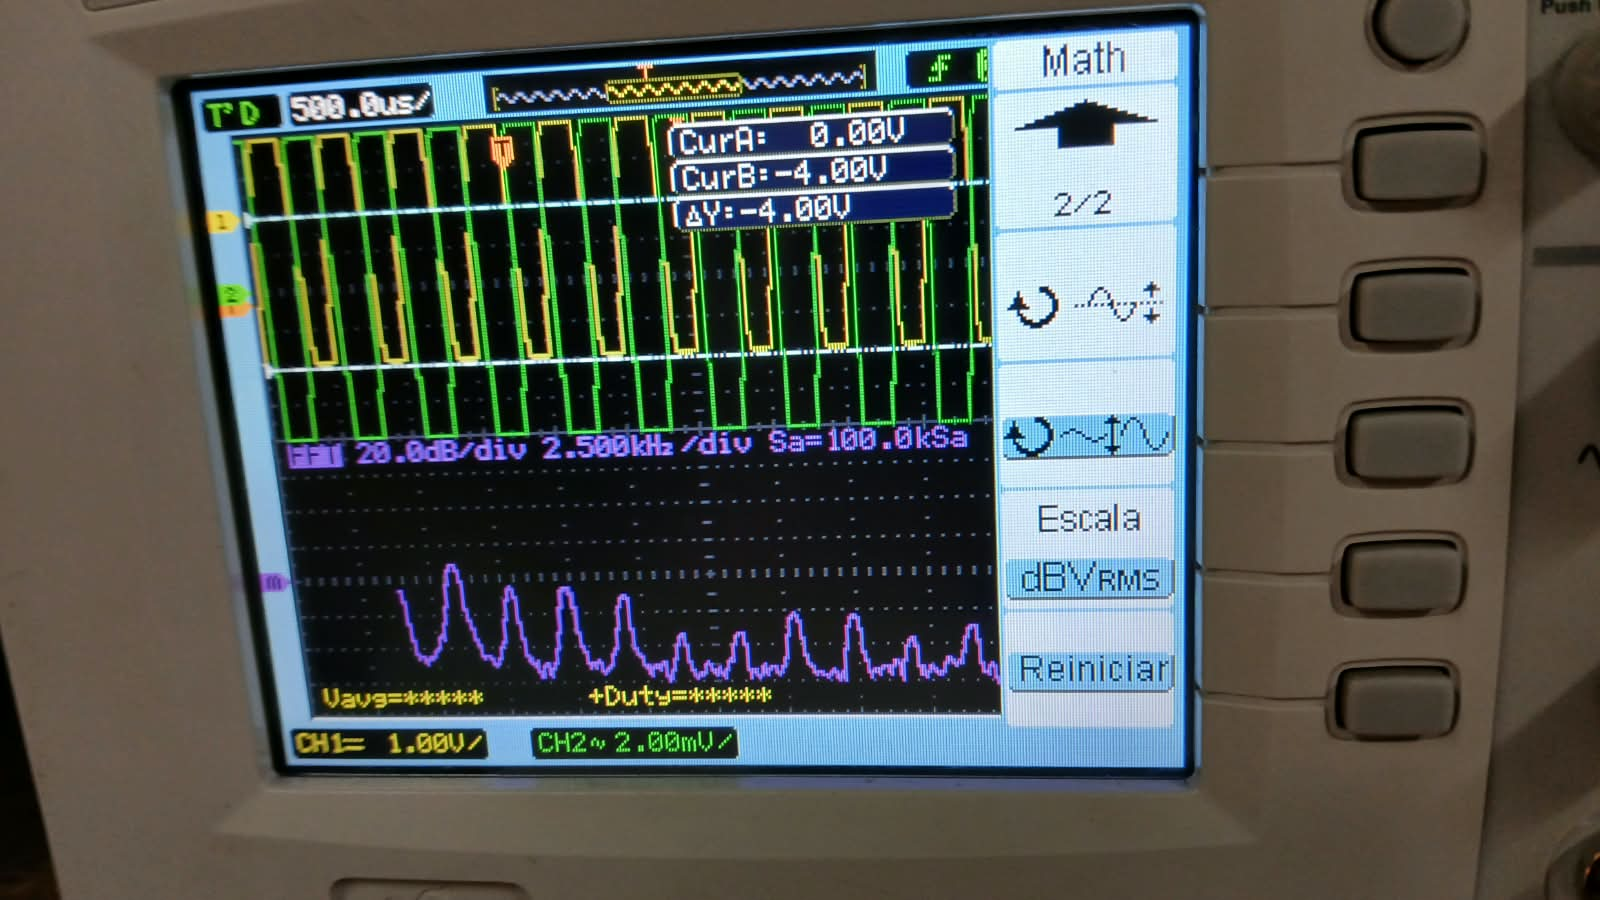
\includegraphics[width=0.8\textwidth]{FotosMed/FFT/Completo/25comzoom.jpeg}
    \caption{Pantalla del Osciloscopio}
    \label{fig:osciloscopioFFTCompleto}
\end{figure}

Se puede ver en \ref{fig:osciloscopioFFTCompleto} una gran distorsion dado que el dispositivo empieza a recortar el semiciclo inferior de la onda.

\subsection{Impedancia De Salida y de entrada}
A continuacion se vera el método de medicion de las impedancias de salida y de entrada para las siguientes configuraciones

Se midio en:
- Etapa 1
- Etapa 1 y 2
- Circuito Completo

\subsubsection{Zout}
Para la medicion de impedancia de salida se trabajó en 2 partes para cada configuracion del equipo en pruebas, se midio la tensión a la salida en vacío y con carga conectada. Para todas las mediciones se utilizo una resistencia conocida de un orden de magnitud similar al esperado en la configuracion en medicion. Una vez obtenidas las mediciones se utilizó la siguiente ecuación:

\[
Z_{\mathrm{out}} = R_L \cdot \left( \frac{V_{\mathrm{vacio}} - V_{\mathrm{carga}}}{V_{\mathrm{carga}}} \right)
\]

Para representar las medicioens se usará como ejemplo la medición de impedancia de salida total.

\begin{figure}[H]
    \centering
    % Primera minipage (ocupa el 45% del ancho de la página)
    \begin{minipage}{0.45\textwidth}
        \centering
        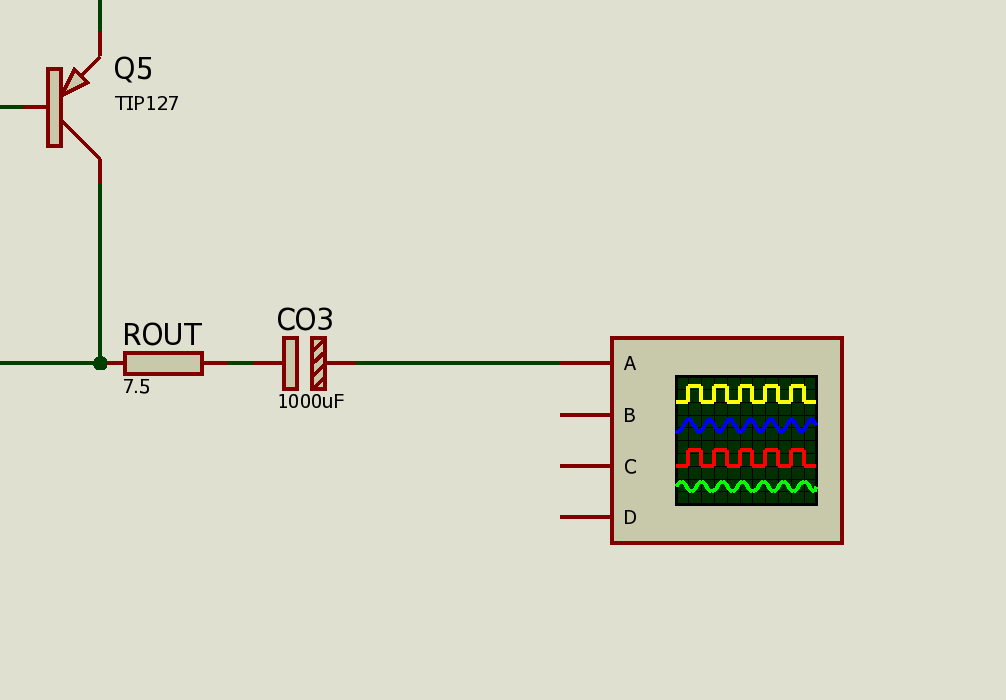
\includegraphics[width=\textwidth]{SetupMediciones/ZOUT/ZoutSinCarga.png} % Ajusta el ancho al de la minipage
        \caption{Representacion esquematica.}
        \label{fig:esquematicpZout}
    \end{minipage}
    \hfill % Relleno elástico para separar las imágenes
    % Segunda minipage (ocupa el 45% del ancho de la página)
    \begin{minipage}{0.45\textwidth}
        \centering
        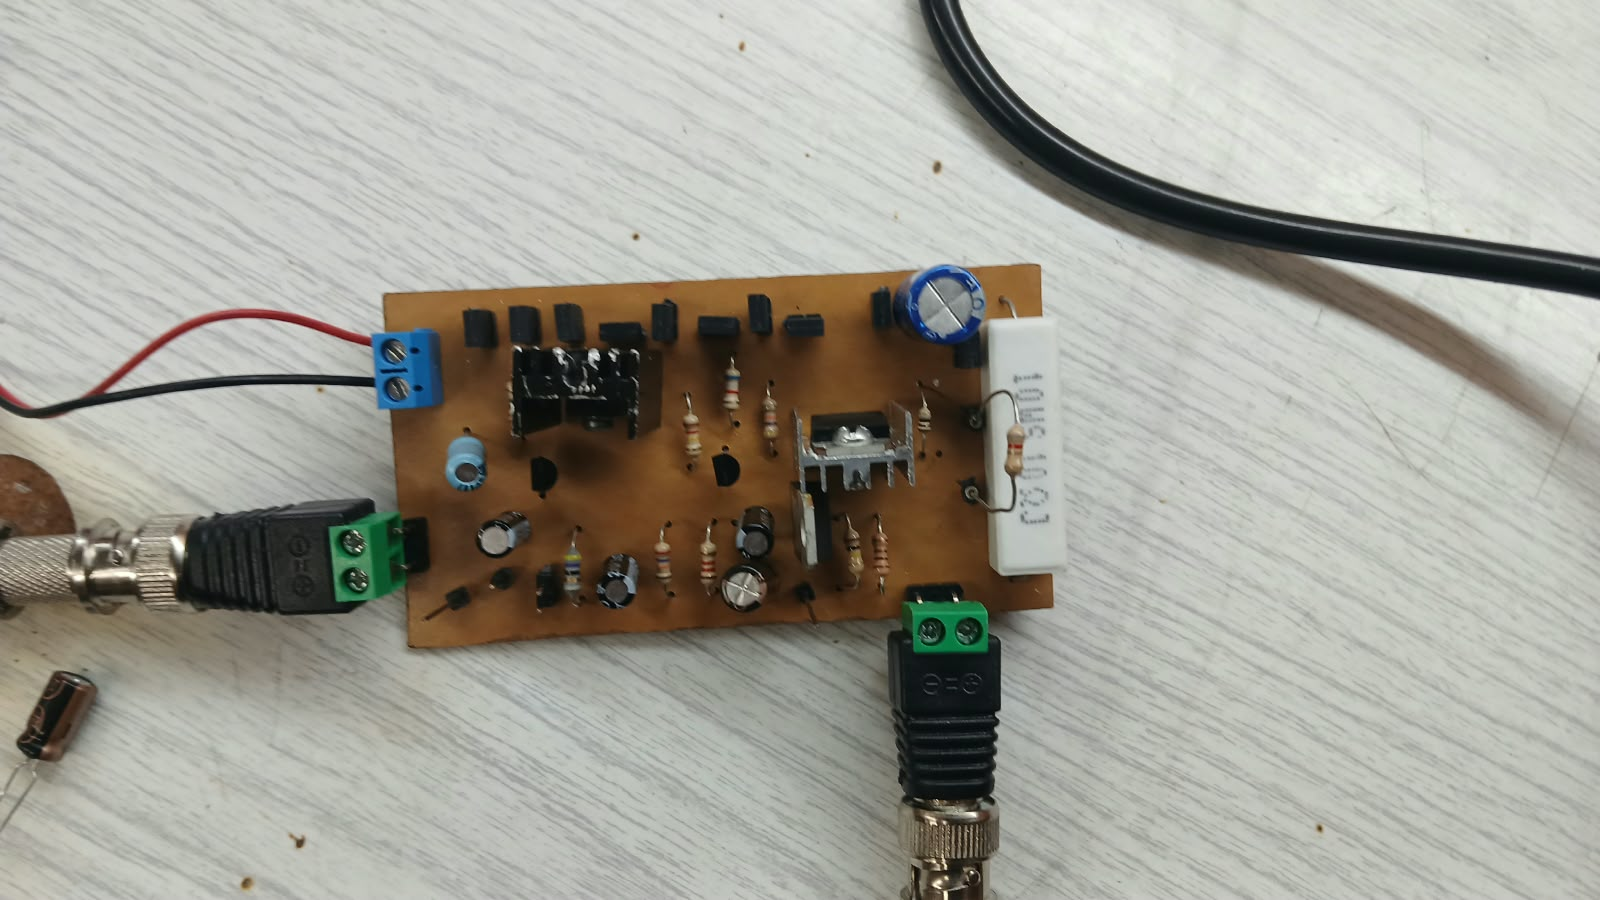
\includegraphics[width=\textwidth]{FotosMed/Impedancias/Zoutmed.jpeg}
        \caption{Setup de la Medicion.}
        \label{fig:medicionZout}
    \end{minipage}
\end{figure}

\begin{figure}[H]
    \centering
    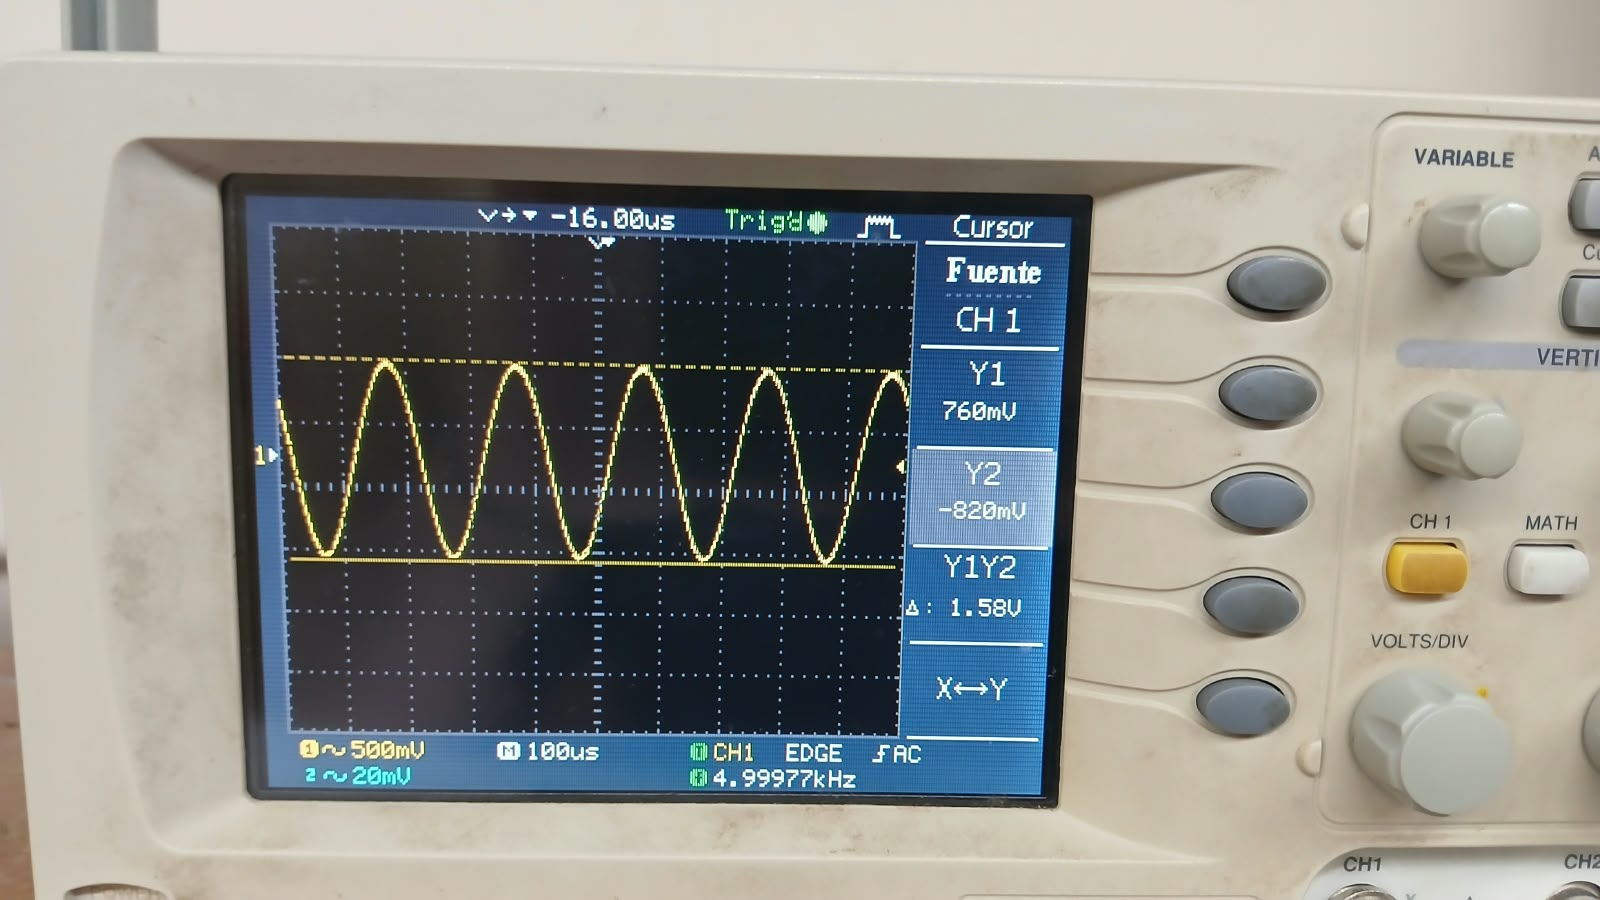
\includegraphics[width=0.8\textwidth]{FotosMed/Impedancias/Zout1.jpeg}
    \caption{Salida del Circuito en Vacio}
    \label{fig:osciloscopiozout}
\end{figure}

En \ref{fig:osciloscopiozout} se muestra el uso de cursores para la medición de tension de salida en vacio. Sigueinte a esta se realizo la medicion del circuito cargado con la Rl.

\begin{figure}[H]
    \centering
    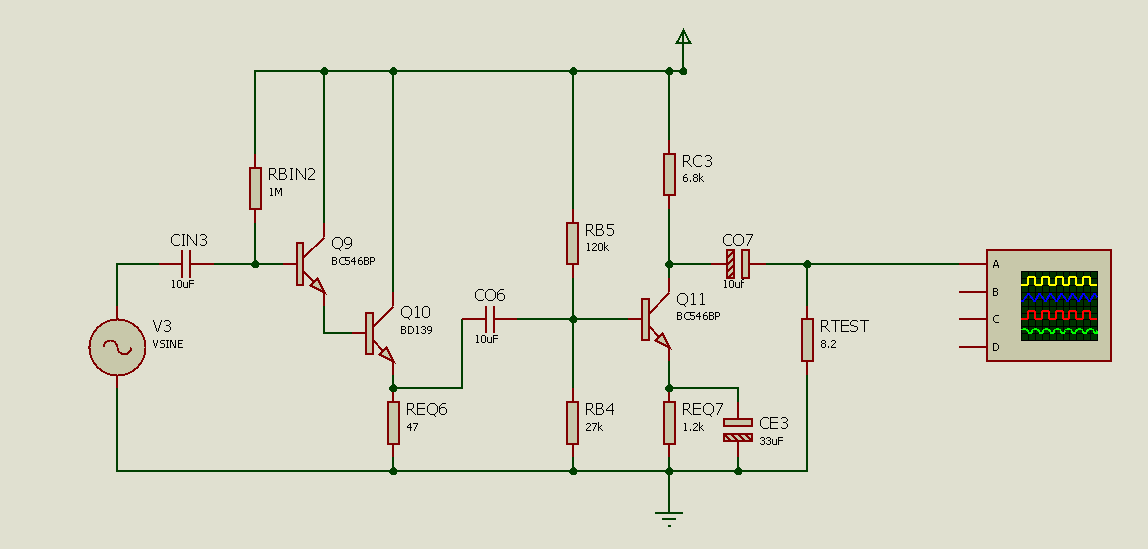
\includegraphics[width=0.8\textwidth]{SetupMediciones/ZOUT/Zout12Cargada.png}
    \caption{Esquema del Circuito Cargado}
    \label{fig:esquemaCargado}
\end{figure}


\begin{figure}[H]
    \centering
    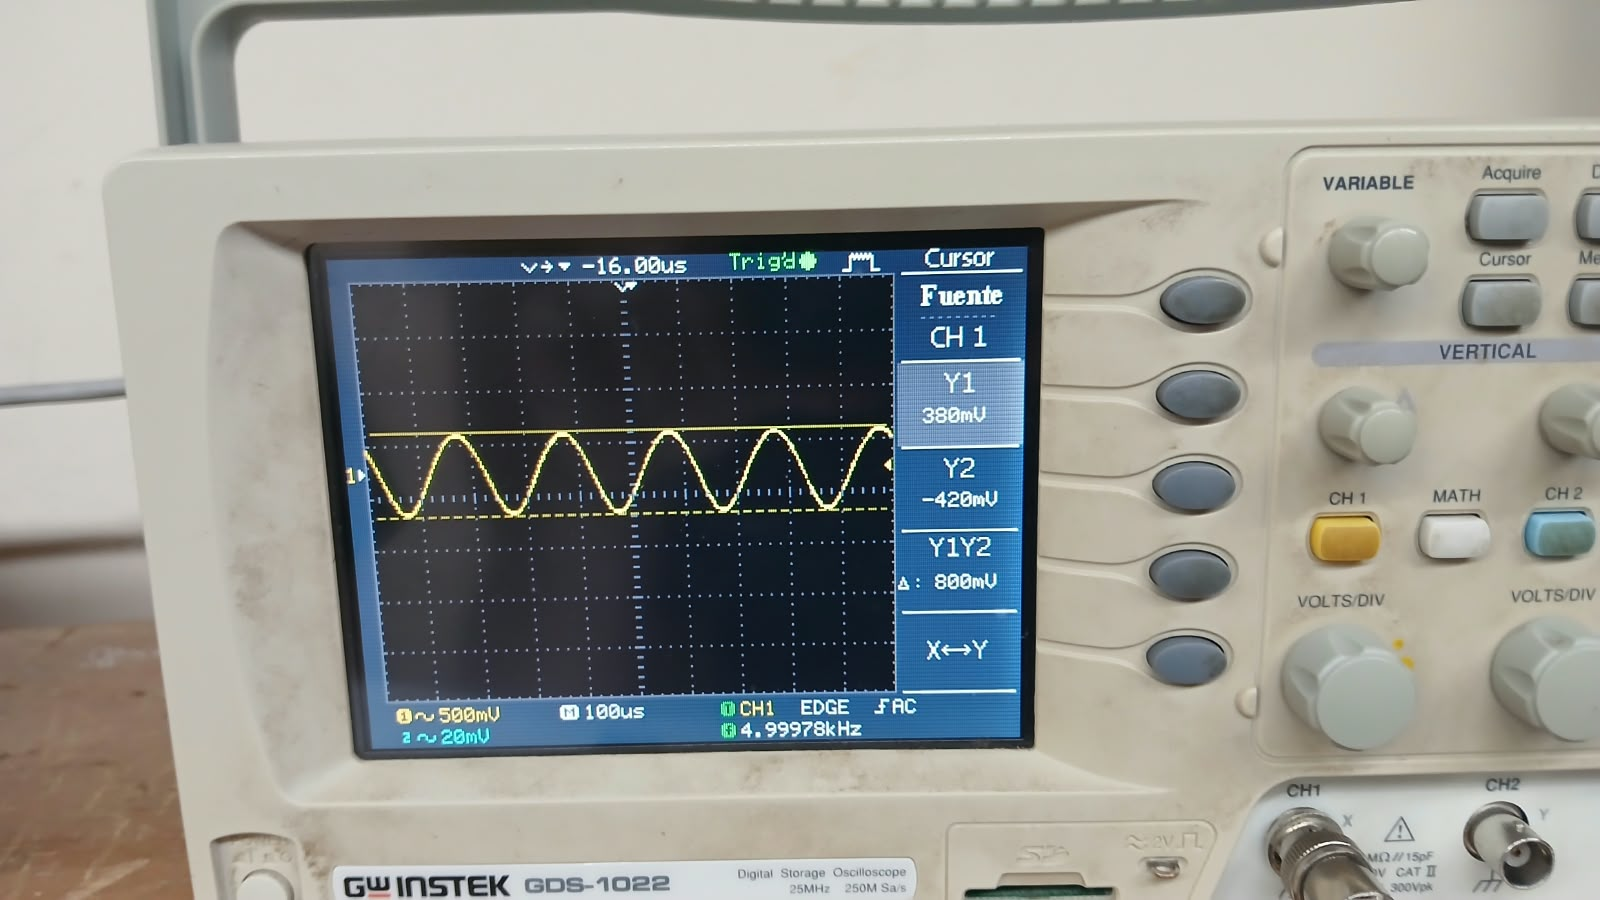
\includegraphics[width=0.8\textwidth]{FotosMed/Impedancias/Zout2.jpeg}
    \caption{Salida del Circuito Cargado}
    \label{fig:osciloscopio2}
\end{figure}

En \ref{fig:osciloscopio2} se muestra la salida del circuito cargado, evidenciandose una disminución de la amplitud de salida.

\subsection{Zin}
Para la medición de la impedancia de entrada el metodo fue diferente, se inyecto la señal atraves de una resistecnia en serie previa a la entrada de una magnitud similar a la impedancia esperada, dado que, si la tensión luego de la resistencia serie es la mitad que la proporcinaba por el generador, entonces la resistencia es exactamente igual a la Impedancia de entrada de la etapa bajo prueba.

Esto ocurre debido a el metodo de divisior de tension:
\[
V_{\mathrm{circuito}} = \frac{V_{\mathrm{gen}}}{2}
\]

Reemplazando esta igualdad en la ecuación original:

\[
\frac{V_{\mathrm{gen}}}{2} = V_{\mathrm{gen}} \cdot \left( \frac{Z_{\mathrm{in}}}{R_S + Z_{\mathrm{in}}} \right)
\]

Simplificando $V_{\mathrm{gen}}$ en ambos miembros dividiendo por $V_{\mathrm{gen}}$:

\[
\frac{1}{2} = \frac{Z_{\mathrm{in}}}{R_S + Z_{\mathrm{in}}}
\]

Se multiplica cruzado para despejar:

\[
R_S + Z_{\mathrm{in}} = 2 \cdot Z_{\mathrm{in}}
\]

Se resta $Z_{\mathrm{in}}$ en ambos lados:

\[
R_S = 2 \cdot Z_{\mathrm{in}} - Z_{\mathrm{in}}
\]

\[
R_S = Z_{\mathrm{in}}
\]

\[
V_{\mathrm{circuito}} = \frac{V_{\mathrm{gen}}}{2}
\]

Se utilizará de ejemplo la medicion de impedancia de entrada total.

\begin{figure}[H]
    \centering
    % Primera minipage (ocupa el 45% del ancho de la página)
    \begin{minipage}{0.45\textwidth}
        \centering
        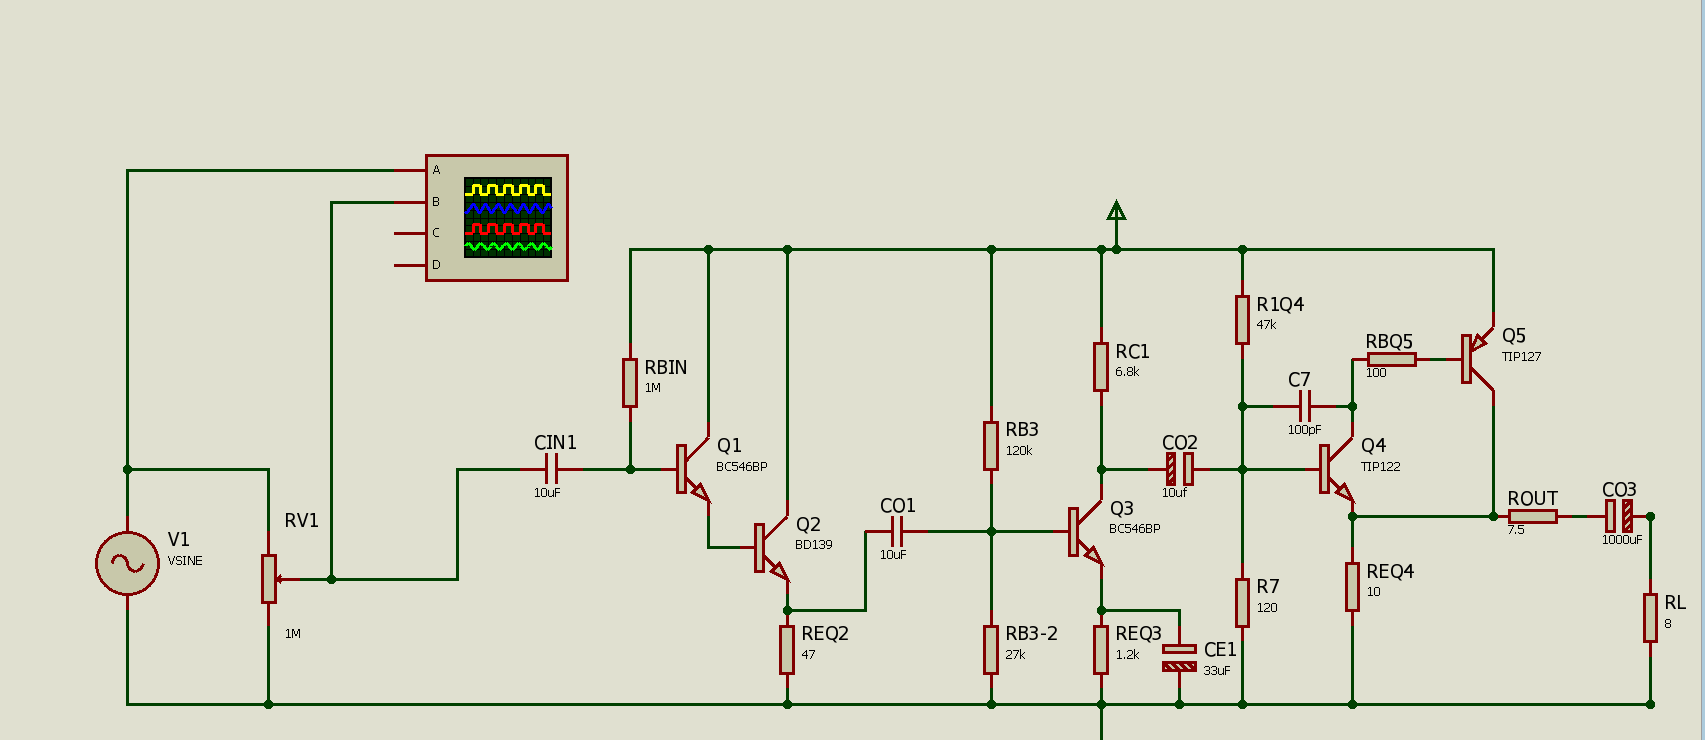
\includegraphics[width=\textwidth]{SetupMediciones/ZIN/ZinTotal.png} % Ajusta el ancho al de la minipage
        \caption{Representación esquemática.}
        \label{fig:esquematicpZin}
    \end{minipage}
    \hfill % Relleno elástico para separar las imágenes
    % Segunda minipage (ocupa el 45% del ancho de la página)
    \begin{minipage}{0.45\textwidth}
        \centering
        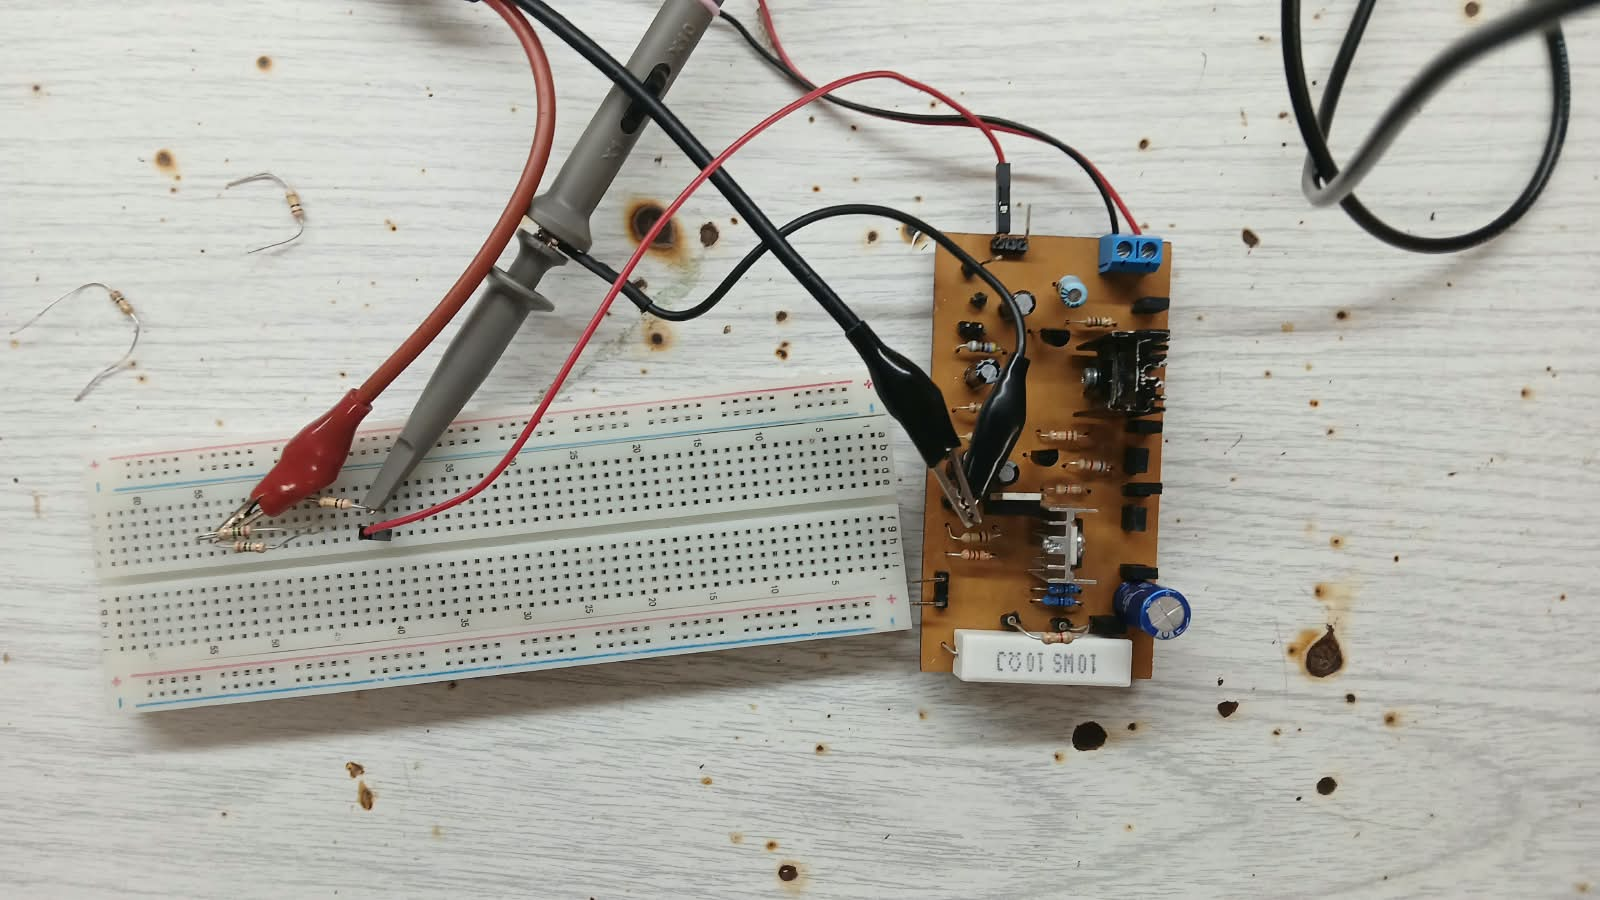
\includegraphics[width=\textwidth]{FotosMed/Impedancias/zinMed.jpeg}
        \caption{Imagen de la Medición.}
        \label{fig:medicionZin}
    \end{minipage}
\end{figure}

Se puede ver en \ref{fig:medicionZin} la utilización de combinaciones de resistencias en paralelo y en serie para encontrar la impedancia de entrada dada la ausencia de un potenciómetro de magnitud acorde.

\begin{figure}[H]
    \centering
    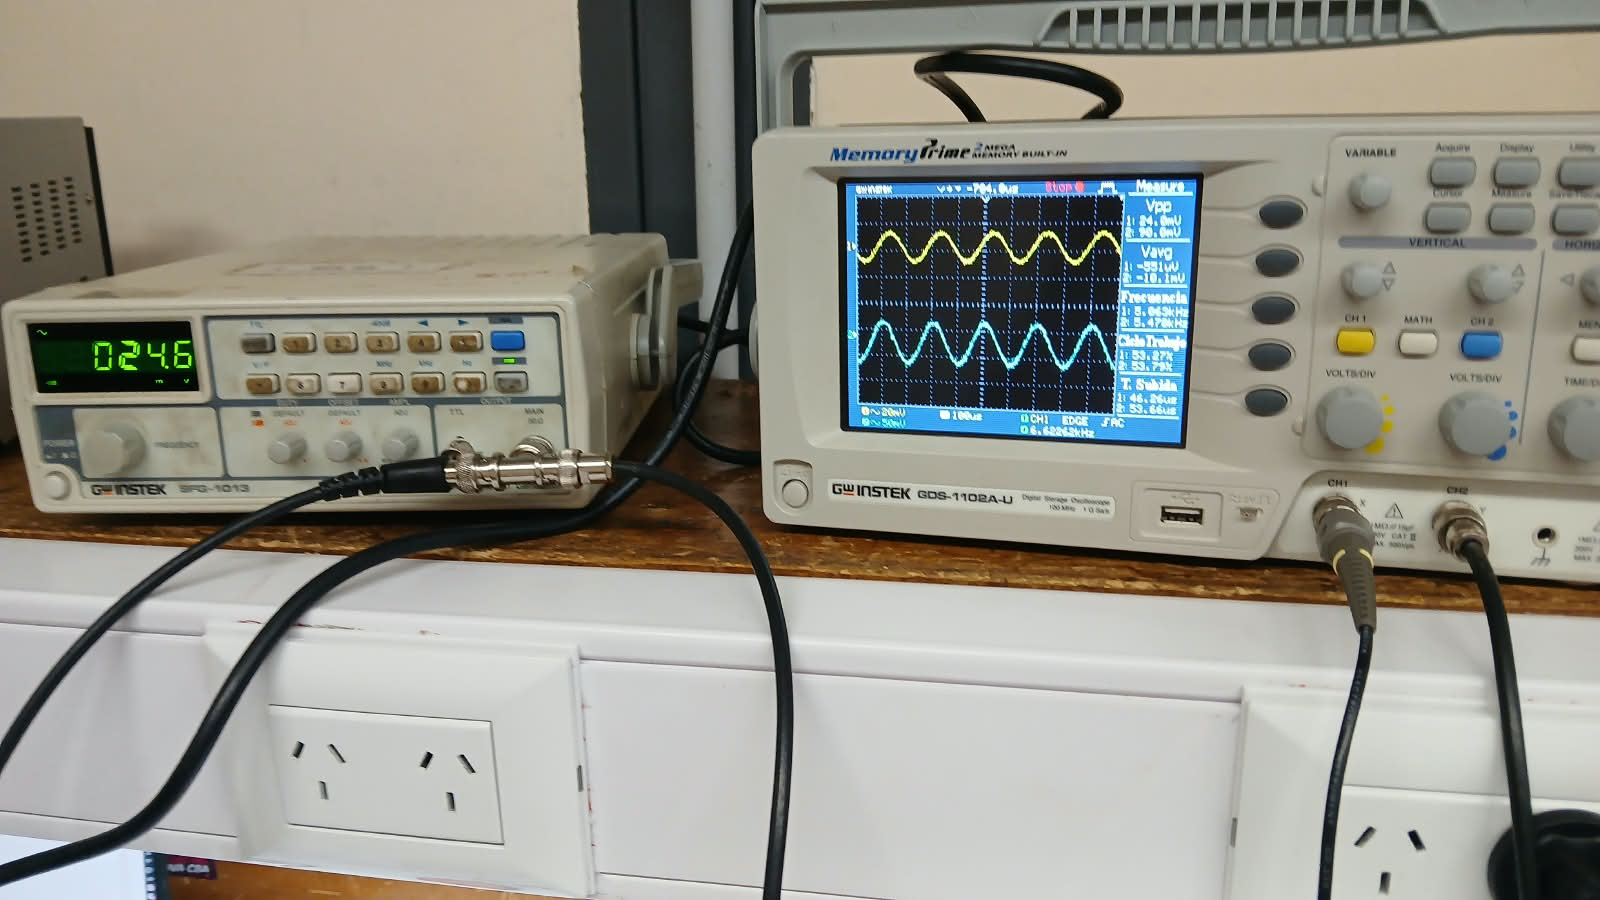
\includegraphics[width=0.8\textwidth]{FotosMed/Impedancias/ZINTOTALSOCLO.jpeg}
    \caption{Pantalla del Osciloscopio}
    \label{fig:osciloscopioZin}
\end{figure}

En \ref{fig:osciloscopioZin} se observa como se utilizaron los instrumentos.

\subsection{Voltaje Máximo de funcionamiento}
Se utilizo la misma configuracion de medicion que en el caso del Barrido de Frecuencia, se mostrara como ejemplo el soporte maximo de tension del circuito total. 

\begin{figure}[H]
    \centering
    % Primera minipage (ocupa el 45% del ancho de la página)
    \begin{minipage}{0.45\textwidth}
        \centering
        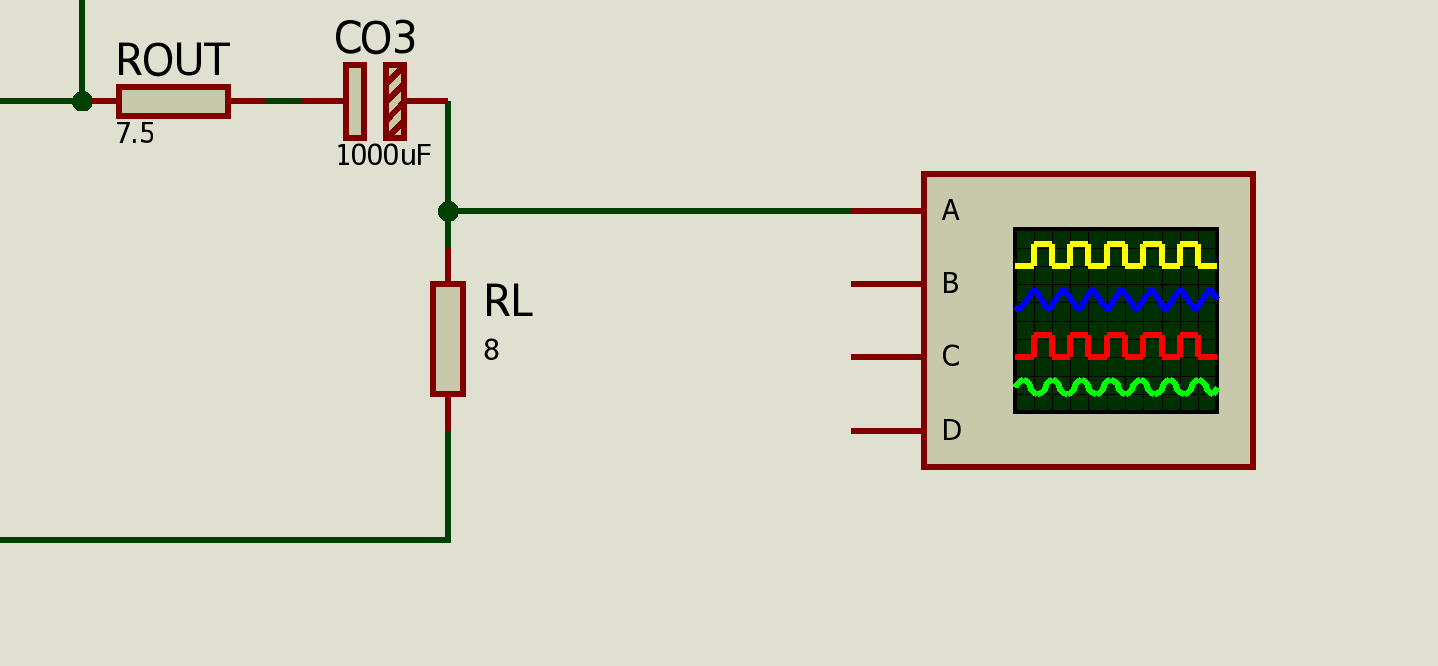
\includegraphics[width=\textwidth]{SetupMediciones/TensionesCorrientes/MaxTension.png} % Ajusta el ancho al de la minipage
        \caption{Representacion esquematica.}
        \label{fig:esquematicpMaxTension}
    \end{minipage}
    \hfill % Relleno elástico para separar las imágenes
    % Segunda minipage (ocupa el 45% del ancho de la página)
    \begin{minipage}{0.45\textwidth}
        \centering
        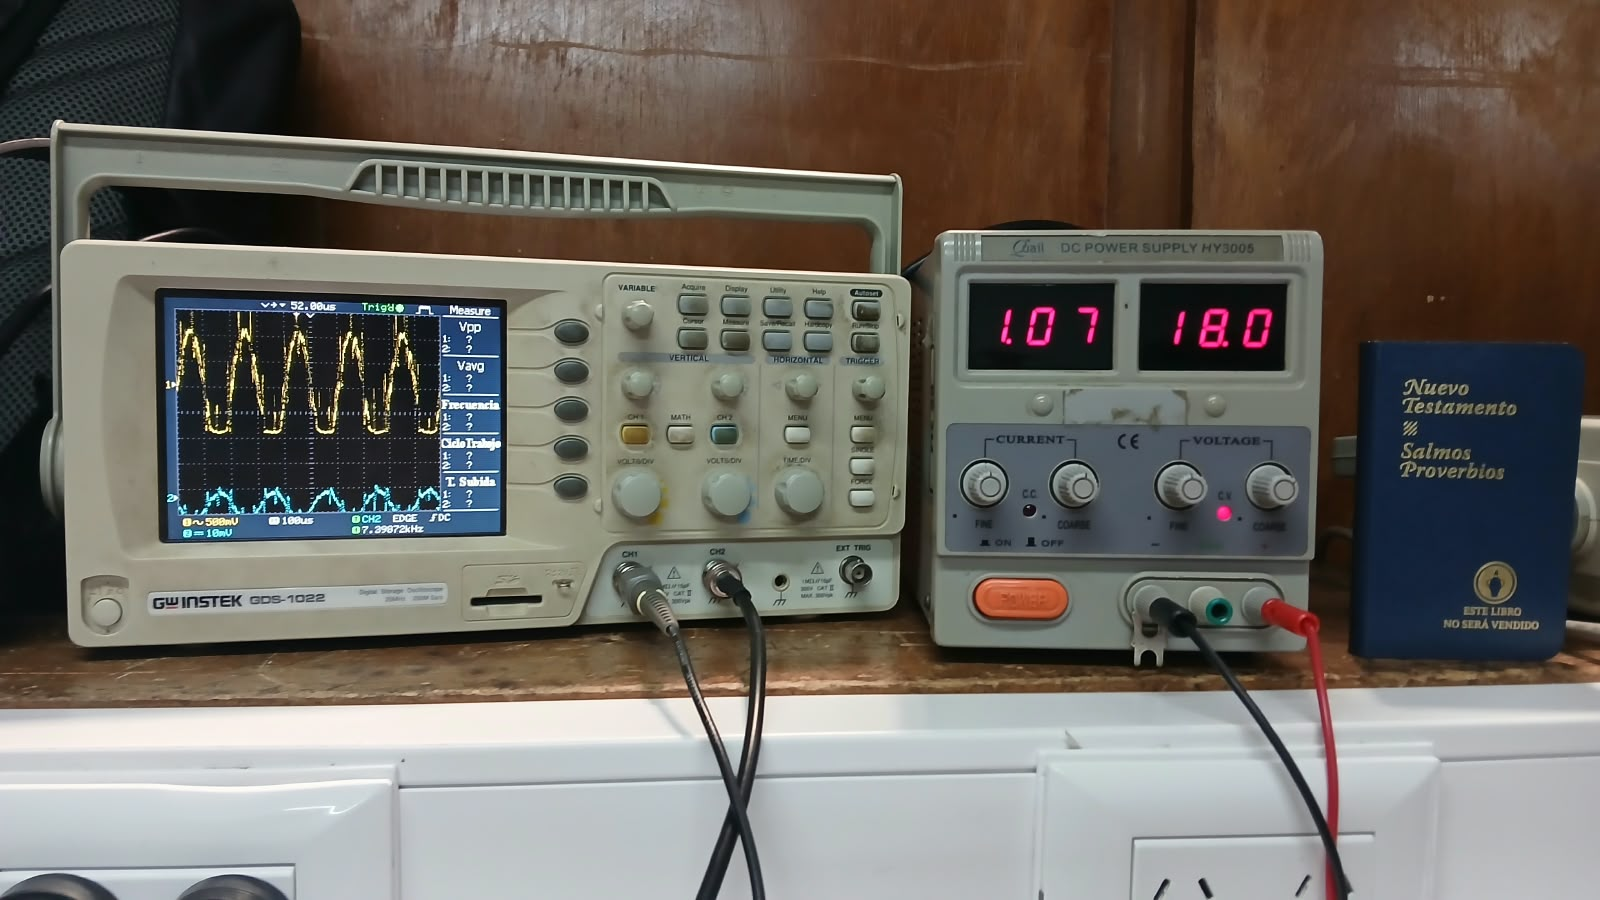
\includegraphics[width=\textwidth]{FotosMed/Voltajesycargademuerte/ARRIBAE123(1).jpeg}
        \caption{Imagen de la Medicion.}
        \label{fig:medicionMAxTension}
    \end{minipage}
\end{figure}

Los 18V en \ref{fig:medicionMAxTension} muestran el voltaje maximo que soporta el circuito, la particularidad de esta medición es que es la tension maxima que soporta el Sziklai, por lo que la maxima tension total esta limitada por la maxima de la última etapa.

\subsection{Voltaje Minimo de funcionamiento}
 Ahora, y con la misma configuracion que la medición anterior, se fue variando la amplitud de la fuente variable y observando la salida por el osciloscopio, el criterio de falla fue no cumplir con el requsito de ganancia. 

 Se usa de ejemplo el circuito total.

\begin{figure}[H]
    \centering
    % Primera minipage (ocupa el 45% del ancho de la página)
    \begin{minipage}{0.45\textwidth}
        \centering
        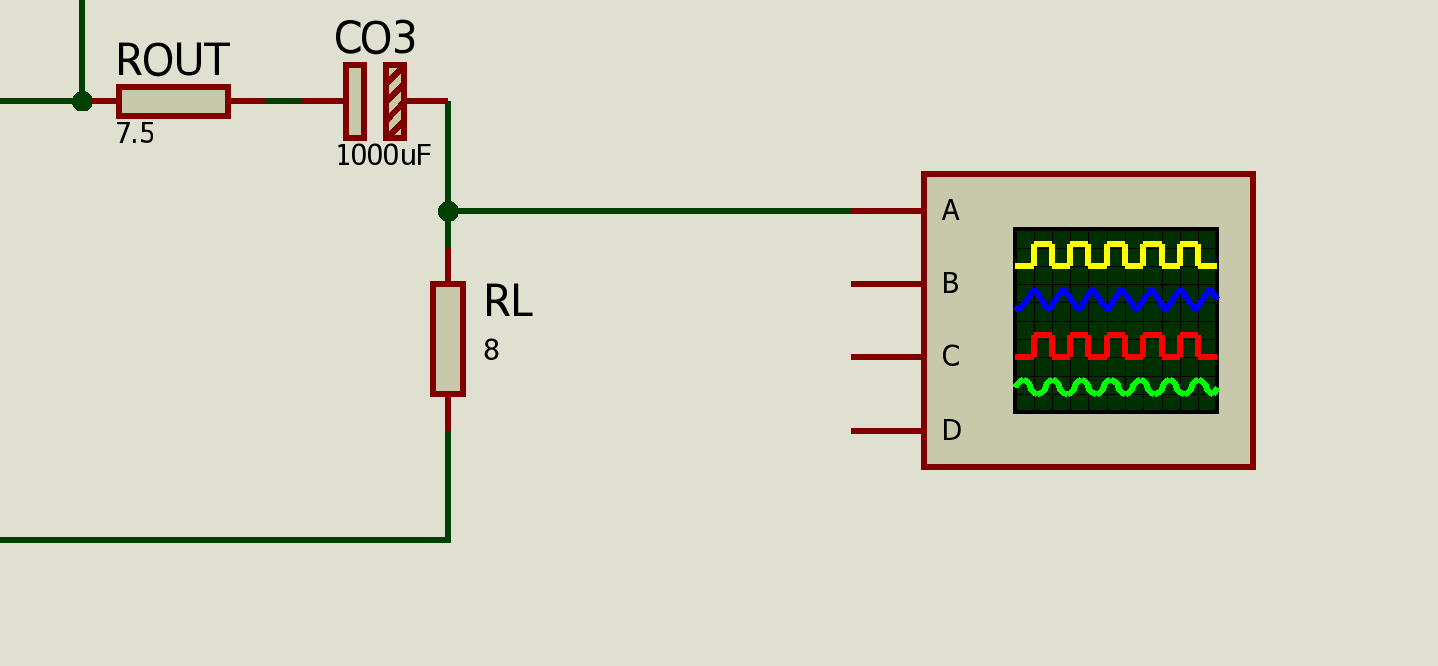
\includegraphics[width=\textwidth]{SetupMediciones/TensionesCorrientes/MaxTension.png} % Ajusta el ancho al de la minipage
        \caption{Representacion esquematica.}
        \label{fig:esquematicpVminimo}
    \end{minipage}
    \hfill % Relleno elástico para separar las imágenes
    % Segunda minipage (ocupa el 45% del ancho de la página)
    \begin{minipage}{0.45\textwidth}
        \centering
        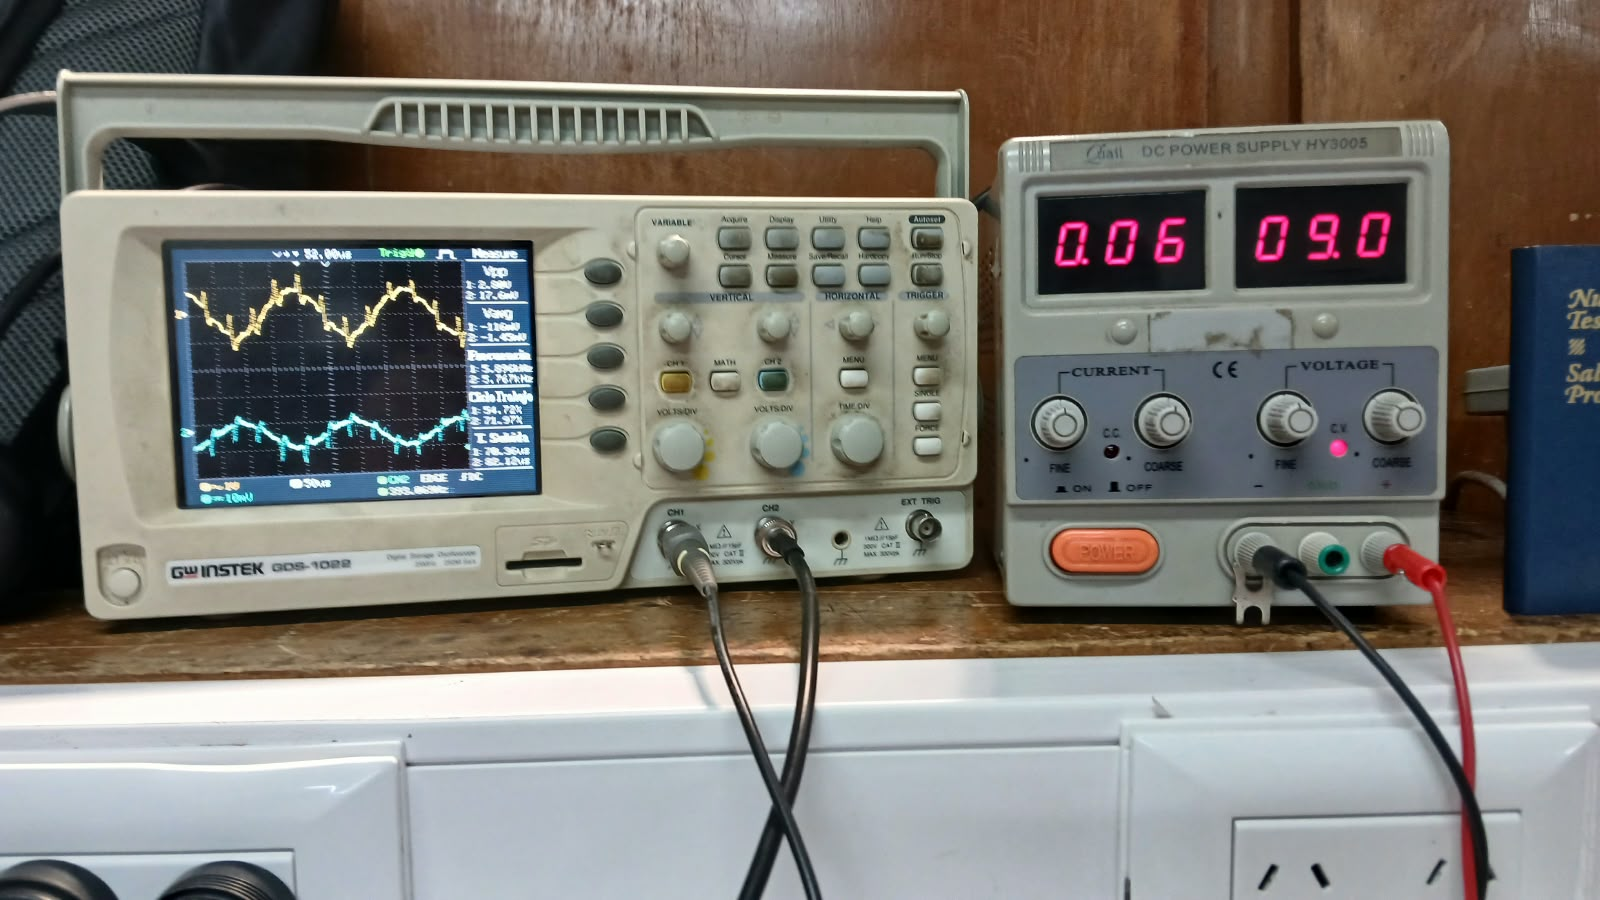
\includegraphics[width=\textwidth]{FotosMed/Voltajesycargademuerte/ABAJOE123(1).jpeg}
        \caption{Imagen de la Medicion.}
        \label{fig:medicionVminimo}
    \end{minipage}
\end{figure}

En \ref{fig:medicionVminimo} se presenta un caso similar a la tensión máxima, el valor de la tensión mínima de funcionamiento esta dado por el valor mínimo de funcionamiento de una de las etapas, en este caso, del emisor común.

\subsection{Resistencia minima de funcionamiento}
Con una configuración parecida a los anteriores, se fueron conectando resistencias en paralelo a la Rl hasta encontrar la resistencias en donde la ganancio no cumple la consigna.

\begin{figure}[H]
    \centering
    % Primera minipage (ocupa el 45% del ancho de la página)
    \begin{minipage}{0.45\textwidth}
        \centering
        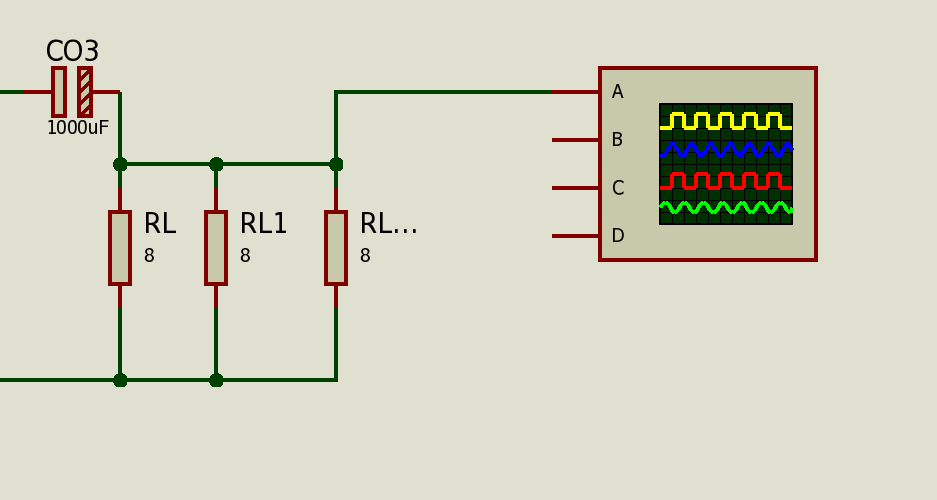
\includegraphics[width=\textwidth]{SetupMediciones/TensionesCorrientes/RdeCorte.png} % Ajusta el ancho al de la minipage
        \caption{Representacion esquematica.}
        \label{fig:esquematicoRCorte}
    \end{minipage}
    \hfill % Relleno elástico para separar las imágenes
    % Segunda minipage (ocupa el 45% del ancho de la página)
    \begin{minipage}{0.45\textwidth}
        \centering
        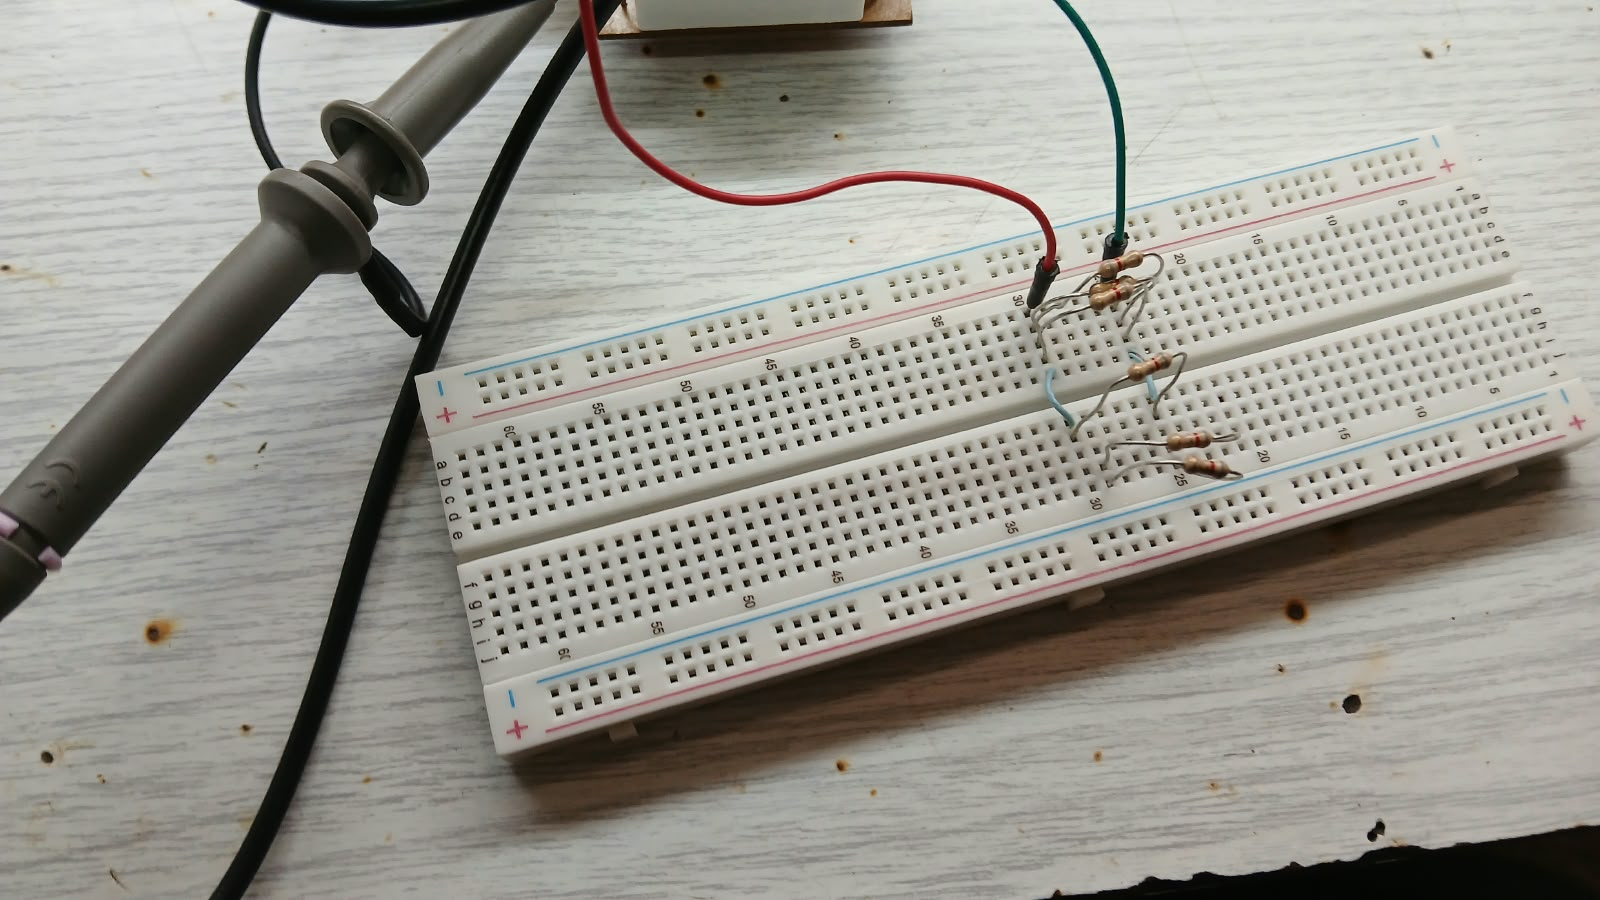
\includegraphics[width=\textwidth]{FotosMed/Voltajesycargademuerte/RMUERTE.jpeg}
        \caption{Imagen de la Medicion.}
        \label{fig:medicionRMuerte}
    \end{minipage}
\end{figure}

\begin{figure}[H]
    \centering
    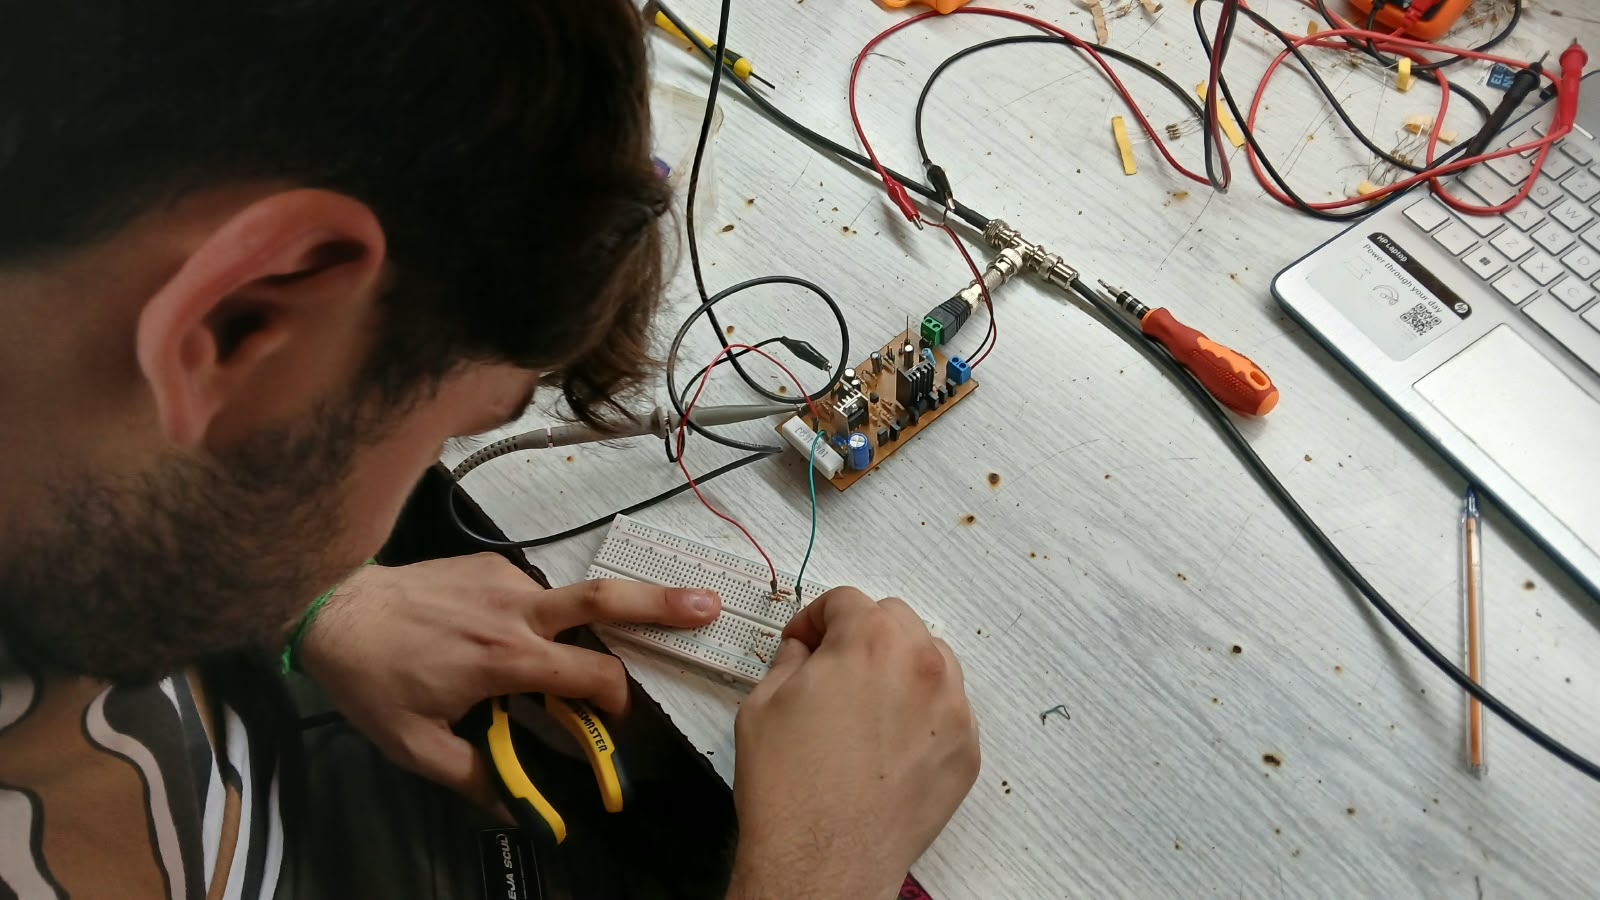
\includegraphics[width=0.8\textwidth]{FotosMed/Voltajesycargademuerte/BuenHombreExplotado.jpeg}
    \caption{Pantalla del Osciloscopio}
    \label{fig:BuenHombreExplotado}
\end{figure}

Se observa en \ref{fig:medicionRMuerte} la disposición de las resistencias de 8.2 Ohm en paralelo, se fueron agregando hasta fallar el requisito de ganancia.


\subsubsection{Depuración del circuito}

La placa del circuito fue diseñada de manera que se pudieran aislar las etapas totalmente en continua y desacoplar las etapas en alterna de forma que se pudiera medir solo el efecto de la primera, la primera cargada con la segunda o todo el amplificador. Esto permitió una fácil depuración del circuito al presentarse fallos.

Originalmente la $R_{cb}$ no estaba incluida en el diseño, lo cual generaba la saturación mencionada. Para definir la ubicación del problema, en principio desconocida, se realizó un procedimiento de medición sectorizado aprovechando las características mencionadas de la placa.

Inicialmente se midieron las condiciones de polarización de cada etapa, dado que se podían aislar completamente, para verificar que la saturación no fuera producto de una polarización incorrecta de algún transistor. 

Descartada esta posibilidad, se midió la salida de cada etapa de amplificación de manera secuencial. Como se mencionó antes, es posible asilar las etapas de amplificación, por lo tanto, se verificó primero el funcionamiento de la etapa Darlington, confirmado su funcionamiento correcto (esta no presentaba saturación y tenía una ganancia de tensión prácticamente unitaria) se acopló la segunda etapa.

El amplificador Emisor Común tampoco presentó problemas, amplificando correctamente, teniendo gran ganancia de tensión y produciendo una inversión de fase. Al acoplar la etapa de salida se pudo ver que era el amplificador Sziklai el cual estaba generando problemas.
Una vez identificado el problema se modificó el circuito añadiendo la $R_{cb}$, que limita la corriente entre colector del transistor npn y la base del pnp.

\subsection{Resultados}

A continuación se presentrán todos los resultados de los valores de diseño, simulación y medición obtenidos en distintas tablas, que irán acompañadas de un breve análisis considerando los objetivos fijados para este circuito.

\begin{table}[H]
\centering
\begin{tabular}{|c|c|c|c|c|c|}
\hline
\textbf{Componente} & \textbf{Parámetro} & \textbf{Diseño [V]} & \textbf{Simulación [V]} & \textbf{Medición [V]} & $\Delta \%$ \\ \hline

% --- BLOQUE Q1 ---
\multirow{4}{*}{Q1} & $V_b$ & 4.85 & 5.20 & 5.47 & -0.05 \\ \cline{2-6}
                             & $V_c$ & 12.00 & 12.00 & 12.00 & 0.00 \\ \cline{2-6}
                             & $V_e$ & 4.15 & 4.20 & 4.87 & -0.14 \\ \cline{2-6}
                             & $I_C$ & 0.71 mA & 0.7 mA & 0.7 mA & 0 \\ \hline

% --- BLOQUE Q2 ---
\multirow{4}{*}{Q2} & $V_b$ & 4.15 & 4.20 & 4.87 & -0.14 \\ \cline{2-6}
                             & $V_c$ & 12.00 & 12.00 & 12.00 & 0.00 \\ \cline{2-6}
                             & $V_e$ & 3.45 & 8.60 & 8.05 & 0.07 \\ \cline{2-6}
                             & $I_C$ & 72.6 mA & 71 mA & 182 mA & -0.61 \\ \hline

% --- BLOQUE Q3 ---
\multirow{4}{*}{Q3} & $V_b$ & 2.20 & 3.40 & 1.10 & 2.09 \\ \cline{2-6}
                             & $V_c$ & 4.86 & 3.40 & 9.00 & -0.62 \\ \cline{2-6}
                             & $V_e$ & 1.27 & 1.52 & 0.56 & 1.71 \\ \cline{2-6}
                             & $I_C$ & 1.05 mA & 1 mA & 0.4 mA & 1.5 \\ \hline

% --- BLOQUE Q4 ---
\multirow{4}{*}{Q4} & $V_b$ & 8.16 & 7.73 & 7.93 & -0.03 \\ \cline{2-6}
                             & $V_c$ & 11.30 & 11.16 & 10.48 & 0.06 \\ \cline{2-6}
                             & $V_e$ & 8.05 & 7.06 & 8.17 & -0.14 \\ \cline{2-6}
                             & $I_C$ & 7.97 mA & 5.5 mA & 3.16 mA & 0.74 \\ \hline

% --- BLOQUE Q5 ---
\multirow{4}{*}{Q5} & $V_b$ & 11.30 & 11.16 & 10.80 & 0.03 \\ \cline{2-6}
                             & $V_c$ & 8.05 & 7.06 & 8.15 & -0.13 \\ \cline{2-6}
                             & $V_e$ & 12.00 & 12.00 & 12.00 & 0.00 \\ \cline{2-6}
                             & $I_C$ & 797 mA & 552 mA & 830 mA & -0.33 \\ \hline

\end{tabular}
\caption{Voltajes de polarización de transistores}
\label{tab:polarizacion}
\end{table}

De la tabla \ref{tab:polarizacion} hay dos conlcusiones de particular importancia. Al ver que no hay gran diferencia entre los valores simulados y medidos en las condiciones de polarización de los transistores, se puede asegurar que estos están trabajando en los puntos de trabajo calculados, lo que hace que el circuto opere en los rangos esperados.

Además, la disipación de potencia está dada principalmente por las corrientes en continua (ya que estas son mayores que las que provoca la señal alterna) por lo que también se confirma que los componentes están dentro de su zona segura de trabajo.

\begin{table}[H]
\centering
\label{tab:potencia_componentes}
\begin{tabular}{|c|c|c|c|c|c|}
\hline
\textbf{Componente} & \textbf{Valor [$\Omega$]} & \textbf{Diseño [mW]} & \textbf{Simulación [mW]} & \textbf{Medición [mW]} & $\Delta \%$ \\ \hline
R_{BD} & 1000000 & 5.10E-02 & 0.049 & 0.002 & 23.5000 \\ \hline
R_{ED} & 47 & 252.7 & 236 & 1400 & -0.8314 \\ \hline
R_{1E} & 120000 & 7.99E-01 & 0.887 & 0.984 & -0.0986 \\ \hline
R_{2E} & 27000 & 1.36E-01 & 0.143 & 0.133 & 0.0752 \\ \hline
R_{CE} & 6800 & 7.4970E+00 & 1.2 & 1.15 & 0.0435 \\ \hline
R_{EE} & 1200 & 1.34E+00 & 10.8 & 0.34 & 30.7647 \\ \hline
R_{1S} & 47000 & 3.13E-01 & 1.2 & 0.291 & 3.1237 \\ \hline
R_{2S} & 100000 & 3.69E-01 & 0.656 & 0.64 & 0.0250 \\ \hline
R_{ES} & 10 & 6482 & 5140 & 6720 & -0.2351 \\ \hline
R_{CB} & 100 & 6.3536 & 10 & 0.001 & 9999.0000 \\ \hline
R_O & 7.5 & 39.018 & 108 & 0 &  \\ \hline
R_L & 8 & 39.018 & 0.04162 & 0 & \\ \hline
Q1 & — & 5.72E+00 & 2.19 & 2.17 & 0.0092 \\ \hline
Q2 & — & 627.2 & 610.73 & 695.24 & -0.1216 \\ \hline
Q3 & — & 3.80E+00 & 2.4 & 3.4 & -0.2941 \\ \hline
Q4 & — & 26.15 & 25.6 & 0.468 & 53.7009 \\ \hline
Q5 & — & 3178 & 3460 & 3080 & 0.1234 \\ \hline
\end{tabular}
\caption{Potencias de cada componente}
\end{table}

El análisis de potencia de cada componente permite una doble comprobación de las condiciones seguras de trabajo de los transistores así como el correcto dimensionamiento de las resistencias utilizadas. Un valor de $\beta$ no previsto por el diseño o la simulación prodría haber provocado un aumento en la corriente de alguna de ellas lo que podría causar su fallo.

\begin{table}[H]
\centering
\begin{tabular}{|c|c|c|c|c|}
\hline
\textbf{Impedancia} & \textbf{Diseño [$\Omega$]} & \textbf{Simulación [$\Omega$]} & \textbf{Medición [$\Omega$]} & $\Delta \%$ \\ \hline
Z_{in} & 327240 & 702000 & 591000 & 0.1878172589 \\ \hline
Z_{out} & 8.0501 & 7.7 & 8.6 & -0.1046511628 \\ \hline
Z_{1IN} & 327240 & 707000 & 491000 & 0.4399185336 \\ \hline
Z_{2IN} & 2148.8 & 2328.00 & & \\ \hline
Z_{23IN} & 2148.8 & 2324 & & \\ \hline
Z_{3IN} & 21061 & 27900 & 27000 & 0.03333333333 \\ \hline
Z_{1OUT} & 31.84 & 0.701 & 5.89 & -0.8809847199 \\ \hline
Z_{2OUT} & 6800 & 5800 & & \\ \hline
Z_{3OUT} & 5.6691 & 7.6 & & \\ \hline
Z_{12IN} & 32724 & 323000 & 494000 & -0.3461538462 \\ \hline
Z_{12OUT} & 6800 & 6800 & 10300 & -0.3398058252 \\ \hline
\end{tabular}
\caption{Impedancias}
\label{tab:impedancias}
\end{table}

Las mediciones, tanto simuladas como reales, de las impedancias del circuito fueron las que precentaron mayores dificultades. El diseño total del amplificador involucró tres etapas: la simulación iterativa de Python, el cálculo de parámetros con Octave y la simulación.

Los resultados obtenidos en Python fueron tomados una vez se corroboraron estos con Octave y luego simulados, sin embargo, en particular las impedancias de entrada y salida globales, precentaban diferencias singinficativas. 

En Octave, el valor de impedancia es el visto en la tabla \ref{tab:impedancias}, que está por debajo del valor adecuado, sin embargo, al ser simulado, se obtuvo un valor que si cumple con los requisitos originales, por lo que se decidió seguir adelante.

Lo mismo sucedió con la impedancia de salida, se obtuvo un valor por debajo de lo requerido pero al simular se vió que si se cumplía con los requerimientos. En este caso el valor visto en la tabla no se corresponde con el valor original.

En vista de las mediciones resultó que, si bien no alcanzaba la misma magnitud, la simulación se correspondía más con el valor medido en la realidad. Esto no ocurrió con el valor de impedancia de salida. Al medir se obtenía un valor de 5.6 Ohms, un valor prácticamente idéntico al obtenido con Octave.

Por esto se optó por modificar el circuito original y reemplazar la $R_O$ de 7.5 Ohms por una de 10, con la que se obtuvieron los valores presentados en la tabla \ref{tab:impedancias}.

Además, debido a un fallo de diseño en la placa, resultaron imposibles de medir de manera adecuada las impedancias de entrada y salida de cada etapa aislada, a excepción de la entrada de la etapa 1 y la salida de la etapa 2.

En estos últimos dos casos, al conectar el generador de señales, este estaba desacoplado en corriente continua mediante un capacitor. Los jumpers ubicados entre etapas para poder desacoplarlas en cambio, no tenían capacitores de desacoplo apropiados para poder inyectar en esos puntos la señal de manera adecuada.

Lo que ocurría era que, al no desacoplar la fuente de alterna de la contínua, su impedancia quedaba en paralelo con la del circuito (entrada o salida según el caso) que se deseaba medir. Como su impedancia, que esá estandarizada, es de 50 Ohms, provocaba una reducción de la impedancia vista en condiciones de continua, moviendo el punto Q a un lugar inapropiado o incluso llevando el transistor al corte o saturación.

Al cambiar de esta forma las conidiciones del circuito, la magnitud de impedancia medida (proceso que, al ser indirecto, conribuye aún más al error) no era la impedancia real del circuito medida en ese punto.

Más allá de estos inconvenientes si se pudieron medir las impedancias de todo el circuito, que son las de mayor interés, y, luego de la modificaión mencionada, ambas resultaron dentro del rango adecuado.

\begin{table}[H]
  \centering
  \begin{tabular}{|c|c|c|c|c|c|c|c|c|}
    \hline
    $f = 5\,\text{kHz}$ & \multicolumn{4}{c|}{$V_{\text{out(p-p)}}$ [mV]} & \multicolumn{4}{c|}{$A_V$} \\ \hline
    $v_{\text{in(p-p)}}$ [mV] & Diseño & Simulación & Medición & $\Delta$ & Diseño & Simulación & Medición & $\Delta$ \\ \hline
    2   & 263.1180  & 192.0  & 232.00  &-0.17 & 131.56 & 96.1   & 116& -0.17 \\ \hline
    5   & 657.7951  & 466.0  & 456.00  &0.02& 131.56 & 93.2   & 91.2& 0.02 \\ \hline
    10  & 1315.5902 & 879.0  & 900.00 &-0.02 & 131.56 & 87.940 & 90&  -0.02 \\ \hline
    15  & 1973.3852 & 1234.0 & 1140.00 & 0.08& 131.56 & 82.33  & 76&  0.08\\ \hline
    17  & 2236.5033 & 1353.0 & 1260.00 &0.07 & 131.56 & 79.59  & 74.12& 0.07\\ \hline
    20  & 2631.1803 & 1468.0 & 1340.00 &0.10 & 131.56 & 73.45  & 67.00& 0.10\\ \hline
    25  & 3288.9754 & 1586.0 & 1360.00 &0.17& 131.56 & 63.45  & 54.40&0.17 \\ \hline
    50  & 6577.9508 & 1600.0 & 2000.00 &-0.20 & 131.56 & 32.1   & 40.00& -0.20\\ \hline
    75  & 9866.9261 & 1411.0 & 2080.00 &-0.32& 131.56 & 18.8   & 27.7320.40 &-0.32 \\ \hline
    100 & 13155.9015& 1243.0 & 2040.00 &-0.39 & 131.56 & 12.4   & 20.40 & -0.39\\ \hline
  \end{tabular}
  \caption{Tensión de Salida vs Entrada del Amplificador Completo}
  \label{tensionGain}
\end{table}

Al analizar los valores obtenidos de tensión y ganancia en la tabla \ref{tensionGain} se puede ver que, si bien hubo ligeros corrimientos en los valores de polarización, el amplificador funciona de manera adecuada dentro de los rangos adecuados y calculados (algo que no resulta redundante recalcar es que la ganancia constante en el Diseño resulta de que se toma como componente lineal al transistor en esta etapa, cosa que no es cierta).

La comparativa Simulación-Medición permite ver que hay ligeras diferencias entre lo esperado y lo encontrado, encontrando las mayores discrepancias entre estas etapas del desarrollo en los 75 y 100 mV, valores muy alejados del rango de operación óptimo del amplificador.

Un valor de particular importancia es el de lso 17 mV, ya que es a partir de este punto que se considera que el amplificador ha perdido su linealidad, lo cual se analizará con mayor detenimiento cuando se vea al THD.

\begin{table}[H]
\centering
\begin{tabular}{|c|c|c|c|}
\hline
\textbf{Frec [Hz]} & \textbf{Total} & \textbf{Etapa 1/2} & \textbf{Etapa 1} \\ \hline
10.00 & 8.36 & 21.27 & 1.00 \\ \hline
100.00 & 55.27 & 127.27 & 0.96 \\ \hline
1000.00 & 159.00 & 283.63 & 0.96 \\ \hline
10000.00 & 163.63 & 287.27 & 1.03 \\ \hline
100000.00 & 161.81 & 240.00 & 0.96 \\ \hline
1000000.00 & 18.90 & 40.72 & 0.94 \\ \hline
3000000.00 & 5.81 & 12.90 & 0.92 \\ \hline
\end{tabular}
\caption{Barrido de frecuencia total ($V_{in} = 10\text{ mV}_{\text{p-p}}$)}
\label{tab:barrido_frec_total}
\end{table}

Los resultados de la tabla \ref{tab:barrido_frec_total} son únicamente de medición. Como se explicó con anterioridad, carece de sentido hacer un barrido en frecuencia preciso en la etapa de diseño, si bien se precentó un gráfico de Bode del amplificador que puede ser acertado en baja frecuencia.

\begin{table}[H]
\centering
\begin{tabular}{|c|c|c|c|}
\hline
\textbf{f} & \textbf{Simulación [KHz]} & \textbf{Medición [KHz]} & $\Delta \%$ \\ \hline
f_l & 1.05 & 0.382 & 1.748691099 \\ \hline
f_h & 3800 & 210.2 & 17.07802093 \\ \hline
BW  & 3800 & 209.8 & 17.11248808  \\ \hline
\end{tabular}
\caption{Frecuencias de Corte y Ancho de Banda}
\label{tab:frecuencias}
\end{table}

Al analizar en conjunto las tablas \ref{tab:barrido_frec_total} y \ref{tab:frecuencias} se puede ver como los resultados de mecidión del barrido en frecuencia permitieron calcular el ancho de banda del amplificador.

En particular en la tabla \ref{tab:frecuencias} se puede ver una gran discrepancia entre lo simulado y lo medido. Si bien el amplificador responde perfectamente (acorde a lo esperado) frente a variaciones de tensión de entrada, no lo hace frente a variaciones en la frecuencia de entrada.

Este fenómeno es debido al efecto Miller. En un principio, al observar como a la salida del amplificador había montada una señal de alta frecuencia a la señal de entrada, se hizo una breve investigación para corregir el error y se colocó un capacitor entre base y colector de Q4, lo cual fue incorrecto.

Al colocar este capacitor de esta manera (se puede ver con más detalle en \cref{Esquematico}) lo que se hace es aumentar la capacidad que existe entre estos terminales, lo que provoca una disminución de la impedancia para las bajas frecuencias. Esto, si bien hace que ya no esté presente el ruido de alta frecuencia (mayor capacidad implica menor impedancia, quedando estas señales con un camino directo a masa) disminuye el ancho de banda.

Este efecto se hace evidente en la tabla \ref{tab:frecuencias} y es debido a que justamente, frecuencias mayores tendrán un camino a masa antes que hacia la salida, lo que para el amplificador singnifica una gran atenuación de estas en la salida. Además se ve que también disminuye la frecuencia de corte inferior, por el mismo fenómeno, para frecuencias menores, la impedancia del amplificador tomará una magnitud lo suficientemente grande como para impedirle el paso a la señal.

\begin{table}[H]
\centering
\begin{tabular}{|c|c|c|c|c|}
\hline
\textbf{$V_{in\text{ p-p}}$ [mV]}& \textbf{Simulación} $\%$& \textbf{Medición} $\%$& $\Delta \%$ \\ \hline
5 & 0.04 & 6.31 & -0.99 \\ \hline
10  & 0.08 & 10.00 & -0.99 \\ \hline
20  & 0.14 & 13.00 & -0.99 \\ \hline
50  & 0.30 & 69.90 & -1.00 \\ \hline
100  & 0.53 & 82.00 & -0.99 \\ \hline
\end{tabular}
\caption{Distorsión armónica total (2 kHz)}
\label{tab:thd_2khz}
\end{table}

\begin{table}[H]
\centering
\begin{tabular}{|c|c|c|c|c|}
\hline
\textbf{$V_{in\text{ p-p}}$ [mV]}  & \textbf{Simulación} $\%$& \textbf{Medición} $\%$& $\Delta \%$ \\ \hline
5 & 0.00 & 0.02 & -1.00 \\ \hline
10 & 0.00 & 1.78 & -1.00 \\ \hline
20 & 0.00 & 6.45 & -1.00 \\ \hline
50  & 0.02 & 3.55 & -0.99 \\ \hline
100 & 0.02 & 9.00 & -1.00 \\ \hline
\end{tabular}
\caption{Distorsión armónica etapa 1 (2 kHz)}
\label{tab:etapa1_thd_2khz}
\end{table}

\begin{table}[H]
\centering
\begin{tabular}{|c|c|c|c|}
\hline
\textbf{$V_{in\text{ p-p}}$ [mV]} & \textbf{Simulación} $\%$& \textbf{Medición} $\%$& $\Delta \%$ \\ \hline
5 & 0.05 & 7.94 & -0.99 \\ \hline
10 & 0.09 & 13.00 & -0.99 \\ \hline
20 & 0.17 & 68.00 & -1.00 \\ \hline
50 & 0.38 & 66.00 & -0.99 \\ \hline
100 & 0.65 & 127.00 & -0.99 \\ \hline
\end{tabular}
\caption{Distorsión armónica etapas 1 y 2 (2 kHz)}
\label{tab:etapas12_thd_2khz}
\end{table}

Al analisar el THD (tablas \ref{tab:thd_2khz}, \ref{tab:etapa1_thd_2khz} y \ref{tab:etapas12_thd_2khz}} es evidente que no fue suficiente el análsis con el simulador no fue suficiente como para estimar su magnitud real. Esto no significa que el funcionamiento del amplificador no sea el adecuado.

Se puede ver que, si bien la magnitud real del THD es mucho mayor que la simulada, tiene un rango adecuado de tensión en el que no precenta un valor mayor al 10$\%$. Como se mencionó al analizar la ganancia en la tabla \ref{tensionGain}, tensión en la que se pierde linealidad es la de 17 mV, dejando un cierto rango de trabajo para el amplificador.

\begin{table}[H]
\centering
\begin{tabular}{|c|c|c|c|c|}
\hline
\textbf{f [Hz]} & \textbf{Total [nV/$\sqrt{\text{Hz}}$]} & \textbf{Etapa 1 [nV/$\sqrt{\text{Hz}}$]} & \textbf{Etapa 2 [nV/$\sqrt{\text{Hz}}$]} & \textbf{Etapa 3 [nV/$\sqrt{\text{Hz}}$]} \\ \hline
10.00 & 59.83 & 3.87 & 60.10 & 59.84 \\ \hline
100.00 & 97.02 & 0.84 & 97.80 & 97.36 \\ \hline
600.00 & 157.35 (Pico Máximo) & 0.77 & 175.42 & 174.48 \\ \hline
1k & 142.84 & 0.77 & 179.23 & 178.15 \\ \hline
2k & 115.63 & 0.77 & 179.78 (Pico Máximo) & 178.53 (Pico Máximo) \\ \hline
10k & 93.15 & 0.77 & 179.28 & 177.94 \\ \hline
100k & 85.87 (Piso de Ruido) & 0.77 & 167.60 & 166.34 \\ \hline
\end{tabular}
\caption{Densidad Espectral de Potencia (PSD) de ruido por etapa en simulación}
\label{tab:psd_ruido}
\end{table}




\newpage

\section{Conclusion}
Summarise what you found and what it implies.

\newpage

\bibliographystyle{ieeetr}
\bibliography{bibliografia}
\newpage

\section{Respuestas a las Preguntas}

\textbf{1. Si la corriente de colector $I_C$ medida en la etapa BJT difiere significativamente del valor de diseño, ¿a qué parámetros del transistor se atribuye esta diferencia? Fundamentar considerando la dispersión de la ganancia de corriente ($\beta$ o $h_{FE}$) y de la tensión base-emisor ($V_{BE}$).}

La diferencia entre la corriente de colector ($I_C$) medida y el valor teórico se debe a que los cálculos analíticos asumen valores nominales. En la realidad física, parámetros intrínsecos como la ganancia de corriente ($\beta$ o $h_{FE}$) y la tensión base-emisor ($V_{BE}$) presentan una notable dispersión originada por tolerancias de fabricación y efectos térmicos.

Por un lado, la ganancia $\beta$ es el parámetro más inestable del dispositivo. En topologías de polarización dependientes, la corriente está dada por $I_C = \beta \cdot I_B$, por lo que cualquier variación en $\beta$ impacta proporcionalmente en $I_C$. 

Por otro lado, la tensión $V_{BE}$ teórica de $0.7\text{ V}$ varía en la práctica entre $0.6\text{ V}$ y $0.75\text{ V}$, experimentando además una deriva térmica de aproximadamente $-2\text{ mV/}^{\circ}\text{C}$. En una red polarizada por divisor de tensión, donde $I_C \approx \frac{V_{BB} - V_{BE}}{R_E}$, cualquier fluctuación en $V_{BE}$ produce un cambio porcentual severo en $I_C$, especialmente si el voltaje de Thévenin en la base ($V_{BB}$) es de baja magnitud.


\textbf{2. En la etapa de entrada formada por $Q_1$ y $Q_2$, ¿cómo influye la configuración Darlington en la estabilidad del punto de trabajo DC ($Q$) ante variaciones de temperatura y dispersión de $\beta$?}

La configuración Darlington ($Q_1$ y $Q_2$) compromete la estabilidad del punto de trabajo en continua ($Q$) debido a su alta sensibilidad térmica y a la severa multiplicación de tolerancias inherentes a los semiconductores.

En primer lugar, frente a las variaciones de temperatura, el arreglo coloca dos uniones base-emisor en serie ($V_{BE(total)} = V_{BE1} + V_{BE2}$). Puesto que cada unión presenta un coeficiente térmico de aproximadamente $-2\text{ mV/}^{\circ}\text{C}$, el conjunto duplica esta deriva a $-4\text{ mV/}^{\circ}\text{C}$, haciendo que el punto $Q$ sea inherentemente más inestable que en una etapa de transistor simple. Adicionalmente, la corriente de fuga térmica del primer transistor ($I_{CBO1}$) ingresa directamente a la base del segundo dispositivo ($Q_2$), el cual la multiplica por su propia ganancia ($\beta_2$). Este fenómeno provoca que, ante incrementos térmicos, la corriente de colector en reposo se desplace significativamente, pudiendo inducir un embalamiento térmico en casos extremos.

Por otro lado, respecto a la dispersión de la ganancia de corriente, el valor total del arreglo resulta del producto de las ganancias individuales ($\beta_{total} \approx \beta_1 \cdot \beta_2$). Esto provoca que las tolerancias de fabricación se multipliquen, generando una variabilidad masiva del parámetro $\beta_{total}$ entre distintos componentes. Debido a esta ganancia combinada tan elevada, la corriente de base ($I_B$) requerida resulta minúscula; en consecuencia, si la red no posee una topología de polarización solida e independiente de $\beta$, el punto $Q$ quedará totalmente a vulnerable a la dispersión del $\beta$.


\textbf{3. ¿Qué función cumple la resistencia $R_{Ein}$ en el emisor de $Q_2$? ¿Qué sucederá con el punto de polarización DC y la excursión de señal si $R_{Ein} = 0$?}

La resistencia $R_{Ein}$ opera como la carga estática de la etapa Darlington. Su función principal radica en establecer el punto de reposo en corriente continua (DC), limitando y fijando la magnitud de la corriente de colector ($I_{CQ}$) al proporcionar un camino resistivo hacia tierra.

En el escenario donde dicha resistencia adopta un valor nulo, el emisor de $Q_2$ queda físicamente cortocircuitado a masa. Bajo esta condición, las uniones base-emisor de los transistores quedarán polarizadas directamente sin ninguna limitación en la malla de salida. En consecuencia, la corriente de colector tenderá a un valor extremo (limitado únicamente por la fuente de alimentación), lo que ocasionará la destrucción térmica de los dispositivos.

\textbf{4. ¿Por qué la ganancia de tensión de esta etapa BJT es sustancialmente mayor que la de un amplificador MOSFET equivalente operando con corrientes de polarización similares? Relacionar con las expresiones de $g_m$ de ambos dispositivos.}

La superioridad en la ganancia de tensión de una etapa BJT frente a un MOSFET equivalente radica en la eficiencia de su transconductancia ($g_m$). Dado que en configuraciones análogas la ganancia es directamente proporcional a este parámetro ($A_v \approx -g_m \cdot R_L$), la diferencia de comportamiento proviene del principio físico rector de cada dispositivo. Al operar bajo la misma corriente de polarización ($I_C = I_D = I_Q$), el BJT exhibe una característica de transferencia exponencial, cuya transconductancia se define como:
$$g_{m,BJT} = \frac{I_C}{V_T}$$
donde $V_T \approx 26\text{ mV}$ a temperatura ambiente. En contraste, el MOSFET obedece a una ley cuadrática regida por campo eléctrico, con una transconductancia expresada como:
$$g_{m,MOSFET} = \frac{2I_D}{V_{OV}}$$
siendo $V_{OV} = V_{GS} - V_{th}$ la tensión de sobreimpulso.

Relacionando matemáticamente ambas expresiones para una misma corriente de polarización $I_Q$, se obtiene el siguiente cociente:
$$\frac{g_{m,BJT}}{g_{m,MOSFET}} = \frac{V_{OV}}{2V_T}$$

Asumiendo un valor típico de operación de $V_{OV} = 0.3\text{ V}$, la relación resulta ser aproximadamente $5.8$. En consecuencia, el BJT ofrece la máxima transconductancia por unidad de corriente posible en semiconductores ($\approx 38.5\text{ mS/mA}$ frente a los típicos $3$ a $8\text{ mS/mA}$ del MOSFET). Esto se traduce en que, ante la misma variación de tensión de entrada, el transistor bipolar genera un cambio de corriente mucho más agresivo, logrando así una ganancia de tensión entre 5 y 10 veces mayor que su contraparte de efecto de campo.

\textbf{5. Analizar el efecto de carga de la segunda etapa ($Q_3$) sobre la primera ($Q_1 - Q_2$). ¿Qué impedancia de entrada presenta la etapa de $Q_3$ ($Z_{in2}$) y cómo afecta a la ganancia en vacío de la primera etapa?}

El análisis del efecto de carga de la segunda etapa ($Q_3$) sobre la primera ($Q_1 - Q_2$) requiere evaluar la impedancia de entrada de la etapa posterior ($Z_{in2}$). De acuerdo con los datos relevados, $Z_{in2}$ presenta un valor  medido de $6.7\text{ k}\Omega$. Por su parte, la primera etapa exhibe una impedancia de salida en vacío ($Z_{out1}$) sumamente baja, con valor de $5.89\ \Omega$ en medición.

Dado que $Z_{in2}$ es varios órdenes de magnitud superior a $Z_{out1}$, el efecto de carga ejercido por $Q_3$ resulta prácticamente despreciable. El impacto sobre la ganancia en vacío de la primera etapa ($A_{v1,0}$) se determina mediante la relación del divisor de tensión conformado por ambas impedancias. La ganancia efectivamente transferida (cargada), denominada $A_{v1}$, se expresa a través de la siguiente ecuación:
$$A_{v1} = A_{v1,0} \cdot \left( \frac{Z_{in2}}{Z_{out1} + Z_{in2}} \right)$$

Al sustituir en la expresión analítica los valores experimentales obtenidos ($Z_{out1} = 5.89\ \Omega$ y $Z_{in2} = 6700\ \Omega$), se determina el factor de transferencia de la red:
$$\frac{Z_{in2}}{Z_{out1} + Z_{in2}} = \frac{6700\ \Omega}{5.89\ \Omega + 6700\ \Omega} \approx 0.9991$$

En consecuencia, la primera etapa transfiere aproximadamente el $99.9\%$ de su señal de tensión a la entrada de $Q_3$. Se concluye así que la ganancia en vacío de la configuración Darlington apenas experimenta atenuación tras la conexión de la segunda etapa amplificadora.

\textbf{6. ¿Por qué modificar la resistencia de colector $R_C$ de la segunda etapa altera drásticamente la ganancia total del amplificador, mientras que modificar $R_{Ein}$ impacta principalmente sobre la impedancia de entrada?}

La alteración de la resistencia de colector ($R_C$) en la segunda etapa ($Q_3$) incide drásticamente sobre la ganancia total del amplificador debido a que dicha etapa opera en configuración de emisor común. En esta topología, la capacidad de amplificación de voltaje es directamente proporcional a la carga resistiva presente en el nodo del colector. Matemáticamente, la magnitud de la ganancia de tensión se rige por la siguiente relación de transferencia dinámica:
$$A_v \approx -g_m \cdot R_C$$
Al alterar $R_C$, se modifica directamente este factor de carga. Un incremento en dicha resistencia permite desarrollar una mayor caída de tensión alterna para una misma variación dinámica en la corriente de colector, alterando de manera directa y lineal la ganancia total de voltaje del sistema.

Por el contrario, la modificación de la resistencia $R_{Ein}$ en la primera etapa afecta primordialmente a la impedancia de entrada, dado que el par Darlington actúa como un seguidor de emisor cuya propiedad fundamental es la transformación de impedancias. La resistencia estática ubicada en el emisor ($R_{Ein}$) se refleja hacia la entrada del circuito (la base de $Q_1$) multiplicada por la ganancia de corriente de ambos semiconductores, aproximándose mediante la expresión:
$$Z_{in} \approx \beta_1 \cdot \beta_2 \cdot R_{Ein}$$
Al modificar $R_{Ein}$, el cambio cuantitativo es amplificado por el producto masivo de las ganancias de corriente ($\beta_1 \cdot \beta_2$). Por consiguiente, el impacto se manifiesta casi exclusivamente sobre la impedancia de entrada total de la red, lo cual determina el nivel de acoplamiento y la exigencia de corriente hacia la fuente de señal, sin aportar ninguna contribución a la ganancia de voltaje.

\textbf{7. Proponer dos modificaciones de diseño para aumentar la ganancia total $G_T$ sin alterar las corrientes de polarización. Evaluar su practicidad de implementación, su impacto en la tensión de excursión simétrica y en la disipación de potencia.}

Dado que las corrientes de polarización deben mantenerse inalteradas, la transconductancia ($g_m$) de los dispositivos permanece constante. Por lo tanto, el incremento de la ganancia total ($G_T$) se debe lograr manipulando exclusivamente la red dinámica de alterna (AC) en la segunda etapa ($Q_3$). La primera modificación consiste en el desacople de la resistencia de emisor ($R_E$) mediante la incorporación de un capacitor paralelo ($C_E$) de alta capacidad. En corriente continua (DC), el capacitor actúa como un circuito abierto, preservando el punto de reposo, la disipación de potencia y la tensión de excursión máxima simétrica sin alteraciones. En alterna, $C_E$ opera como un cortocircuito a masa, suprimiendo la realimentación negativa (degeneración de emisor) y elevando la ganancia a su valor intrínseco de lazo abierto:
$$A_v \approx -g_m \cdot R_C$$
Esta solución presenta una alta practicidad de implementación, siendo una maniobra estándar, económica y simple que requiere únicamente el agregado de un componente pasivo.

La segunda alternativa radica en reemplazar la resistencia de colector ($R_C$) por una carga activa, implementada convencionalmente mediante un espejo de corriente con transistores PNP. Esta red inyecta la corriente de polarización nominal exacta, manteniendo el punto de reposo DC inalterado, pero exhibe una impedancia dinámica ($r_o$) extremadamente elevada frente a señales de pequeña amplitud. En consecuencia, la ganancia de tensión se dispara a niveles máximos según la expresión:
$$A_v \approx -g_m \cdot r_o$$
Sin embargo, su practicidad es moderada a baja en ensambles con componentes discretos, dado que exige semiconductores adicionales rigurosamente apareados. En cuanto a sus impactos, si bien la disipación de potencia estática global no varía de forma significativa, la excursión simétrica se ve reducida; el transistor de la carga activa requiere una caída de tensión mínima (voltaje de saturación, $V_{CE(sat)}$) para operar en su región lineal, lo que sustrae margen de voltaje respecto al riel de alimentación y comprime el límite antes de alcanzar el recorte de la señal.

\textbf{8. La especificación requiere $Z_{in} > 350\text{ k}\Omega$. ¿Por qué resulta indispensable utilizar el par Darlington ($Q_1 - Q_2$) en lugar de una etapa Emisor Común convencional para cumplir este requerimiento?}

Para alcanzar una impedancia de entrada superior a $350\text{ k}\Omega$, resulta inviable emplear una etapa de emisor común con un único transistor debido a sus limitaciones estructurales. En dicha topología, la impedancia base depende del parámetro $h_{ie}$ y de la reflexión de la resistencia de emisor, aproximándose como $Z_{in} \approx \beta \cdot R_E$. Dado que la ganancia de corriente ($\beta$) estándar oscila entre 100 y 300, satisfacer la especificación exigiría un valor de $R_E$ tan elevado que demandaría voltajes de alimentación impracticables o corrientes de polarización microscópicas, degradando severamente la linealidad del sistema; esto sin mencionar que el divisor resistivo de polarización en paralelo mermaría aún más la impedancia neta. Por el contrario, el uso del par Darlington configurado como colector común (seguidor de emisor) se torna indispensable porque multiplica las ganancias de corriente de ambos semiconductores ($\beta_{total} \approx \beta_1 \cdot \beta_2$). Esta multiplicación extrema permite que la carga dinámica en el emisor se refleje hacia la entrada por un factor masivo, elevando la impedancia intrínseca del circuito al rango de los mega-ohmios mediante la relación:
$$Z_{in} \approx \beta_1 \cdot \beta_2 \cdot R_E$$
De este modo, el acoplamiento supera ampliamente el requerimiento de diseño sin comprometer la estabilidad del punto de reposo ni las características de transferencia de la etapa amplificadora.

\textbf{9. Si el generador de funciones del laboratorio presenta una impedancia de salida de $50\ \Omega$, ¿por qué la caída de tensión en dicha resistencia interna es despreciable frente a la $Z_{in}$ medida?}

La interacción entre la fuente de señal y el amplificador se rige por el principio del divisor de tensión, donde la resistencia interna del generador ($R_g = 50\ \Omega$) y la impedancia de entrada del amplificador ($Z_{in}$) quedan configuradas en serie. La tensión efectiva que ingresa a los terminales de la primera etapa ($V_{in}$) se determina a partir de la siguiente ecuación de transferencia:
$$V_{in} = V_g \cdot \left( \frac{Z_{in}}{R_g + Z_{in}} \right)$$
donde $V_g$ representa la tensión electromotriz ideal de la fuente. Dado que la impedancia de entrada lograda por la topología Darlington (del orden de los cientos de kilo-ohmios) es masivamente superior a la resistencia del generador ($Z_{in} \gg R_g$), el denominador de la expresión está dominado enteramente por $Z_{in}$. Al evaluar el divisor, el factor de acoplamiento resulta prácticamente unitario ($\approx 0.9998$). Matemáticamente, esto implica que más del $99.98\%$ de la señal se transfiere de forma íntegra hacia la base del primer transistor, limitando la caída de tensión sobre la resistencia interna a un nivel inferior al $0.02\%$. En consecuencia, esta pérdida resulta de una magnitud absolutamente despreciable, garantizando que la etapa de entrada opere de forma análoga a un voltímetro ideal, es decir, sensando la tensión sin introducir atenuación ni demandar corriente significativa al instrumental de laboratorio.

\textbf{10. La especificación exige una impedancia de salida $Z_o = 8\ \Omega \pm 5\%$ para alimentar una carga $R_L = 8\ \Omega$. ¿Qué característica del circuito permite lograr un valor tan bajo de $Z_o$ y qué ocurriría con la ganancia si se conectara $R_L$ directamente al colector de un Emisor Común?}

El cumplimiento de esta especificación se sustenta en el diseño de la etapa de potencia, la cual emplea un par Sziklai configurado funcionalmente como un amplificador de corriente. Esta topología permite dividir la impedancia proveniente de la etapa amplificadora de tensión previa por el producto de las ganancias de corriente de los transistores de potencia ($\beta_1 \cdot \beta_2$). Como resultado, se obtiene una impedancia de salida intrínseca del semiconductor extraordinariamente baja, del orden de los miliohmios, lo cual permite al diseñador fijar con precisión la impedancia de salida final del amplificador ($Z_o = 8\ \Omega$) mediante la adición de componentes resistivos pasivos en serie con la carga. Por el contrario, si la carga de baja impedancia ($R_L = 8\ \Omega$) se conectara directamente al nodo del colector de una etapa en emisor común, la ganancia de tensión del sistema colapsaría. En dicha topología, la ganancia es directamente proporcional a la resistencia de carga efectiva en alterna, rigiéndose por la ecuación:
$$A_v \approx -g_m \cdot (R_C \parallel R_L)$$
Al conectar una carga tan exigente, el paralelo equivalente se desploma a un valor cercano a los $8\ \Omega$ (independientemente del valor de $R_C$), destruyendo la capacidad del circuito para desarrollar una amplitud de voltaje significativa y atenuando severamente la señal.

\textbf{11. Al incrementar paulatinamente el nivel de tensión de entrada $v_{in}$, la salida comienza a distorsionarse. ¿Qué mecanismo del BJT limita la excursión máxima por el extremo superior (positivo) y cuál por el extremo inferior (negativo) en la etapa de salida?}

La distorsión asimétrica en los extremos de la señal se explica por la naturaleza intrínseca del transistor bipolar, cuyo comportamiento de transferencia emula la curva exponencial de un diodo ($i_C \approx I_S \cdot e^{v_{BE}/V_T}$). Por el extremo que conduce a la saturación, la excursión está limitada por el incremento drástico de la conducción; al elevarse la excitación, el punto de operación alcanza una zona donde la pendiente de la curva exponencial de la unión base-emisor se vuelve extremadamente pronunciada (casi vertical). En esta región, un incremento infinitesimal en la tensión de entrada exige un aumento masivo de corriente que la red de polarización no puede suministrar, forzando a que la tensión colector-emisor colapse abruptamente a su límite físico mínimo ($V_{CE(sat)}$) y achatando el pico de la onda. Por el extremo opuesto, la limitación es gobernada por el mecanismo de corte; cuando el semiciclo de la señal reduce la polarización por debajo del umbral de conducción de la unión (ingresando a la región donde la curva exponencial del diodo se aplana asintóticamente a cero), la corriente de colector se anula ($I_C = 0$). Bajo esta condición, el dispositivo deja de conducir y la tensión de salida queda rígidamente enclavada, cercenando el otro extremo de la señal alterna.



\textbf{12. A partir de la relación exponencial $i_C = I_S \cdot e^{v_{be}/V_T}$, explicar por qué el BJT genera distorsión armónica ante amplitudes de entrada pequeñas (decenas de mV) y cómo contribuye la resistencia de emisor no puenteada ($R_{E1}$) a linealizar la respuesta.}

La generación de distorsión armónica en un transistor BJT tiene su origen en la naturaleza no lineal de su característica de transferencia, regida por la relación exponencial $i_C = I_S \cdot e^{v_{be}/V_T}$. Al someter la unión a una señal senoidal y expandir la función mediante series de Taylor, la corriente resultante se compone de un término fundamental y de múltiples sumandos de orden superior que originan los armónicos. Para que dichas componentes sean despreciables, la amplitud debe respetar estrictamente la condición de pequeña señal ($v_{be} \ll V_T \approx 26\text{ mV}$); sin embargo, cuando la excitación alcanza decenas de milivoltios, el cociente $\frac{v_{be}}{V_T}$ adquiere un peso matemático significativo, deformando la onda de salida. Para mitigar este fenómeno, la inclusión de una resistencia de emisor no puenteada ($R_{E1}$) introduce una realimentación negativa local que modifica la transconductancia efectiva de la etapa según la expresión:
$$g_m' = \frac{g_m}{1 + g_m R_{E1}}$$
Al garantizar por diseño que $g_m R_{E1} \gg 1$, este parámetro dinámico se independiza de la no linealidad del semiconductor y se aproxima a $g_m' \approx \frac{1}{R_{E1}}$. En consecuencia, la transferencia de la etapa ($i_c \approx \frac{v_{in}}{R_{E1}}$) pasa a estar gobernada exclusivamente por un componente pasivo lineal, lo que suprime drásticamente la distorsión armónica del sistema.

\textbf{13. ¿A partir de qué amplitud de tensión de entrada la distorsión de la señal se hizo perceptible en el osciloscopio? Relacionar dicha medición con el valor de THD obtenido y el umbral de detección visual ($3\% \text{--} 5\%$).}

Durante el ensayo de laboratorio, la deformación de la señal se hizo perceptible a simple vista al alcanzar una tension de $18\text{ mV}_{pp}$. Dado que el protocolo de ensayo fue estipulado el registro de la Distorsión Armónica Total (THD) en niveles de tensión predefinidos, la caracterización espectral se tomó sobre el escalón de los $20\text{ mV}_{pp}$, arrojando un valor de distorsión del $13\%$. Esta correlación concuerda con las limitaciones de resolución del ojo humano. Por consiguiente, se infiere que al cruzar la frontera de los $18\text{ mV}_{pp}$, el contenido armónico de la señal rompió dicha barrera crítica del $5\%$, volviéndose evidente.

\textbf{14. ¿Qué componente del circuito presenta la mayor disipación de potencia en reposo ($P_{DC}$)? Justificar mediante las mediciones de $V_{CE}$ e $I_C$, y verificar si opera dentro de su Zona de Operación Segura (SOA).}

El análisis del balance energético indica que, si bien la resistencia $R_{ES}$ registra el mayor consumo absoluto del circuito con $6.72\text{ W}$[cite: 1], el componente activo que presenta la mayor disipación de potencia en reposo ($P_{DC}$) es el transistor $Q_5$, alcanzando un valor medido de $3.08\text{ W}$. Esta magnitud térmica se justifica analíticamente mediante el producto de sus coordenadas estáticas de polarización, calculándose como $P_{DC} = V_{CE} \cdot I_C$. Al proyectar estos parámetros operativos (correspondientes a un $V_{CE}$ de $3.95\text{ V}$ y una $I_C$ de $0.779\text{ A}$) sobre la gráfica de la Zona de Operación Segura (SOA) estipulada en la hoja de datos del fabricante, se constata que el punto de trabajo estático se ubica firmemente dentro de los márgenes térmicos y eléctricos permitidos. Esto garantiza que el dispositivo opera exento de riesgos por ruptura o fatiga térmica, dado que cuenta con un disipador térmico  adecuado para evacuar los $3.08\text{ W}$ generados hacia el ambiente.

\textbf{15. Al reducir la tensión de alimentación $V_{CC}$ por debajo de los $12\text{ V}$ nominales, ¿cuál es el primer parámetro que se degrada (ganancia de tensión, excursión máxima sin recorte o impedancias)? Fundamentar.}

Al reducir la tensión de alimentación ($V_{CC}$) por debajo de su valor nominal, el primer parámetro que experimenta una degradación drástica es la excursión máxima de señal. Este fenómeno se debe a que la amplitud máxima de la onda está físicamente delimitada por el nivel de tensión de los rieles de la fuente; al disminuir $V_{CC}$, el espacio disponible para que la señal oscile se comprime, provocando que la onda alcance prematuramente las zonas de saturación o corte y sufra un recorte severo. 



\end{document}